\documentclass[11pt,a4paper]{article}
\usepackage[utf8]{inputenc}
\usepackage[T1]{fontenc}
\usepackage{lmodern}
\usepackage{textcomp}
\usepackage{amsmath,amssymb}
\usepackage{graphicx}
\usepackage{booktabs}
\usepackage{longtable}
\usepackage{array}
\usepackage{listings}
\usepackage{xcolor}
\usepackage[margin=1in]{geometry}
\usepackage{float}
\usepackage[hidelinks,breaklinks]{hyperref}
\usepackage{microtype}
\setlength{\parskip}{4pt}
\lstset{basicstyle=\ttfamily\scriptsize,breaklines=true,breakatwhitespace=false,
  postbreak=\mbox{\textcolor{gray}{$\hookrightarrow$}\space},frame=single,
  framerule=0.3pt,rulecolor=\color{gray!60},columns=fullflexible,keepspaces=true,
  showstringspaces=false,numbers=none,xleftmargin=4pt,xrightmargin=4pt,
  literate={\_}{{\_}}1}
\graphicspath{{figures/}}
\providecommand{\tightlist}{}
\title{Supplementary material: Joint BBN and X-ray Constraints on keV Sterile-Neutrino Dark Matter, 2024--2026}
\author{HEP-Genesis-Agent session record \\ \small Project: ramp-research-sterile-bbn-xray}
\date{2026-11-02}
\begin{document}
\maketitle
\noindent\textit{\small Supplementary material, generated mechanically from the session record: it lists exactly what ran, in order, without interpretation.}
\vspace{1em}



\appendix
\section{Implementation details}
\label{app:impl}
This appendix is generated mechanically from the session record; it lists exactly what ran, in order, without interpretation.
\subsection{Session}
\begin{itemize}
  \item Source: cli client; conversation \texttt{644f1997}
  \item Started: 2026-10-21 11:01:50; report generated: 2026-11-02 17:04:43
  \item Project: ramp-research-sterile-bbn-xray (\texttt{/\allowbreak{}Users/\allowbreak{}nramachandra/\allowbreak{}hep-genesis-testing/\allowbreak{}projects/\allowbreak{}ramp-research-sterile-bbn-xray})
  \item Compute execution site(s) selected in the session: local
  \item 3 user turn(s), 352 tool call(s) (10 returned errors), 20 figure(s), 29 data file(s)
\end{itemize}
\subsection{Models}
\begin{longtable}{@{}p{0.16\textwidth}p{0.34\textwidth}p{0.44\textwidth}@{}}
\toprule Stage & Model & Endpoint \\ \midrule \endhead
quick & \texttt{muse-spark-bf16} & \texttt{https:\allowbreak{}/\allowbreak{}/\allowbreak{}inference-api.alcf.anl.gov/\allowbreak{}resource\_\allowbreak{}server/\allowbreak{}minerva/\allowbreak{}api/\allowbreak{}v1} \\
report & \texttt{muse-spark-bf16} & \texttt{https:\allowbreak{}/\allowbreak{}/\allowbreak{}inference-api.alcf.anl.gov/\allowbreak{}resource\_\allowbreak{}server/\allowbreak{}minerva/\allowbreak{}api/\allowbreak{}v1} \\
coder & \texttt{muse-spark-bf16} & \texttt{https:\allowbreak{}/\allowbreak{}/\allowbreak{}inference-api.alcf.anl.gov/\allowbreak{}resource\_\allowbreak{}server/\allowbreak{}minerva/\allowbreak{}api/\allowbreak{}v1} \\
\bottomrule\end{longtable}
\subsection{MCP servers}
\begin{longtable}{@{}p{0.22\textwidth}p{0.12\textwidth}p{0.6\textwidth}@{}}
\toprule Server & Transport & Location \\ \midrule \endhead
hep-research-aid & stdio & \texttt{python -m hep\_\allowbreak{}genesis.domain.mcp\_\allowbreak{}server} \\
alcf-tools & stdio & \texttt{python -m hep\_\allowbreak{}genesis.iri.alcf.mcp\_\allowbreak{}server} \\
nersc-tools & stdio & \texttt{python -m hep\_\allowbreak{}genesis.iri.nersc.mcp\_\allowbreak{}server} \\
paper-search & stdio & \texttt{uvx --with mcp\textless{}\allowbreak{}2 paper-search-mcp} \\
web-search & stdio & \texttt{uvx duckduckgo-mcp-server} \\
cosmic-emulators & http & \texttt{https:\allowbreak{}/\allowbreak{}/\allowbreak{}cosmic.77-42-88-84.sslip.io/\allowbreak{}mcp} \\
\bottomrule\end{longtable}
\subsection{Tool-call log}
Chronological; arguments and results are truncated for space (the full record is in the project's \texttt{provenance/} folder).
\begin{longtable}{@{}p{0.04\textwidth}p{0.22\textwidth}p{0.36\textwidth}p{0.32\textwidth}@{}}
\toprule \# & Tool & Arguments & Outcome \\ \midrule \endhead
1 & \texttt{hep-research-aid}\newline\texttt{list\_\allowbreak{}agent\_\allowbreak{}files} & \texttt{\{\}\allowbreak{}} & \texttt{[]\allowbreak{}} \\
2 & \texttt{hep-research-aid}\newline\texttt{list\_\allowbreak{}input\_\allowbreak{}files} & \texttt{\{\}\allowbreak{}} & \texttt{\{   ''status'':\allowbreak{} ''success'',\allowbreak{}   ''files'':\allowbreak{} []\allowbreak{},\allowbreak{}   ''usage'':\allowbreak{} ''Pass any of these filenames to load\_\allowbreak{}table\_\allowbreak{}data()\allowbreak{}.'' \}\allowbreak{}} \\
3 & \texttt{hep-research-aid}\newline\texttt{list\_\allowbreak{}datasets} & \texttt{\{\}\allowbreak{}} & \texttt{\{'count':\allowbreak{} 0,\allowbreak{} 'datasets':\allowbreak{} []\allowbreak{}\}\allowbreak{}} \\
4 & \texttt{hep-research-aid}\newline\texttt{list\_\allowbreak{}files} & \texttt{\{\}\allowbreak{}} & \texttt{Files in .:\allowbreak{}   - .git   - .gitignore   - .last-release-seen   - ISSUES.md   - SCOPE.md   - docs   - downloads   - logs   - projects   - reports   - research-results   - runs   - scripts   - venvs   - w\ldots{}\allowbreak{}} \\
5 & \texttt{hep-research-aid}\newline\texttt{get\_\allowbreak{}dispatch} & \texttt{\{\}\allowbreak{}} & \texttt{Dispatch:\allowbreak{} local execution.} \\
6 & \texttt{serve-sbbn.sh}\newline\texttt{list\_\allowbreak{}sterile\_\allowbreak{}nu\_\allowbreak{}skills} & \texttt{\{\}\allowbreak{}} & \texttt{\{   ''status'':\allowbreak{} ''ok'',\allowbreak{}   ''files'':\allowbreak{} []\allowbreak{},\allowbreak{}   ''message'':\allowbreak{} ''2 skills. Load one with load\_\allowbreak{}sterile\_\allowbreak{}nu\_\allowbreak{}skill.'',\allowbreak{}   ''metadata'':\allowbreak{} \{     ''skills'':\allowbreak{} \{       ''kev-sterile-dm-xray'':\allowbreak{} ''keV sterile-neutrino dark matter \textbackslash{}\allowbreak{}u2014 \ldots{}\allowbreak{}} \\
7 & \texttt{local}\newline\texttt{search\_\allowbreak{}arxiv\_\allowbreak{}abstracts} & \texttt{\{''query'':\allowbreak{} ''sterile neutrino dark matter X-ray constraints 3.5 keV line 2024'',\allowbreak{} ''max\_\allowbreak{}results'':\allowbreak{} 8\}\allowbreak{}} & \texttt{[1702.08430v1]\allowbreak{} keV sterile neutrino Dark Matter Abstract:\allowbreak{} We give an overview of the current status of keV sterile neutrino Dark Matter. After a short introduction,\allowbreak{} we start by a general discussion of\ldots{}\allowbreak{}} \\
8 & \texttt{local}\newline\texttt{search\_\allowbreak{}arxiv\_\allowbreak{}abstracts} & \texttt{\{''query'':\allowbreak{} ''sterile neutrino big bang nucleosynthesis helium deuterium constraints mixing'',\allowbreak{} ''max\_\allowbreak{}results'':\allowbreak{} 8\}\allowbreak{}} & \texttt{[1706.03138v1]\allowbreak{} Introduction to Big Bang Nucleosynthesis and Modern Cosmology Abstract:\allowbreak{} Primordial nucleosynthesis remains as one of the pillars of modern cosmology. It is the testing ground upon which\ldots{}\allowbreak{}} \\
9 & \texttt{local}\newline\texttt{search\_\allowbreak{}arxiv\_\allowbreak{}abstracts} & \texttt{\{''query'':\allowbreak{} ''keV sterile neutrino dark matter parameter space status review'',\allowbreak{} ''max\_\allowbreak{}results'':\allowbreak{} 8\}\allowbreak{}} & \texttt{[1702.08430v1]\allowbreak{} keV sterile neutrino Dark Matter Abstract:\allowbreak{} We give an overview of the current status of keV sterile neutrino Dark Matter. After a short introduction,\allowbreak{} we start by a general discussion of\ldots{}\allowbreak{}} \\
10 & \texttt{hep-research-aid}\newline\texttt{search\_\allowbreak{}arxiv} & \texttt{\{''query'':\allowbreak{} ''sterile neutrino dark matter X-ray XRISM eROSITA NuSTAR constraints'',\allowbreak{} ''max\_\allowbreak{}results'':\allowbreak{} 10,\allowbreak{} ''sort\_\allowbreak{}by'':\allowbreak{} ''submittedDate''\}\allowbreak{}} & \texttt{Found 10 papers matching query:\allowbreak{} 'sterile neutrino dark matter X-ray XRISM eROSITA NuSTAR constraints' (source:\allowbreak{} arXiv API)\allowbreak{}  Paper 1:\allowbreak{} arXiv ID:\allowbreak{} 2610.28633v1 Title:\allowbreak{} Constraints on Millimeter-wave Extraga\ldots{}\allowbreak{}} \\
11 & \texttt{hep-research-aid}\newline\texttt{search\_\allowbreak{}arxiv} & \texttt{\{''query'':\allowbreak{} ''sterile neutrino dark matter lepton asymmetry resonant production BBN constraint'',\allowbreak{} ''max\_\allowbreak{}results'':\allowbreak{} 10,\allowbreak{} ''sort\_\allowbreak{}by'':\allowbreak{} ''submittedDate''\}\allowbreak{}} & \texttt{Found 10 papers matching query:\allowbreak{} 'sterile neutrino dark matter lepton asymmetry resonant production BBN constraint' (source:\allowbreak{} arXiv API)\allowbreak{}  Paper 1:\allowbreak{} arXiv ID:\allowbreak{} 2610.28633v1 Title:\allowbreak{} Constraints on Millimeter\ldots{}\allowbreak{}} \\
12 & \texttt{local}\newline\texttt{web\_\allowbreak{}search} & \texttt{\{''query'':\allowbreak{} ''arXiv 2024 2025 sterile neutrino dark matter X-ray limits XRISM eROSITA NuSTAR mixing angle''\}\allowbreak{}} & \texttt{Sterile neutrinos offer a minimal and testable explanation for dark matter (DM)\allowbreak{},\allowbreak{} with their radiative decay actively searched for in X-ray observations. We show that cold sterile neutrino DM can be ef\ldots{}\allowbreak{}} \\
13 & \texttt{local}\newline\texttt{search\_\allowbreak{}arxiv\_\allowbreak{}abstracts} & \texttt{\{''max\_\allowbreak{}results'':\allowbreak{} 8,\allowbreak{} ''query'':\allowbreak{} ''NuSTAR eROSITA blank sky decaying sterile neutrino limits''\}\allowbreak{}} & \texttt{[1606.02684v1]\allowbreak{} Neutrino Oscillations With Two Sterile Neutrinos Abstract:\allowbreak{} This work estimates the probability of \$$\mu$\$ to \$e\$ neutrino oscillation with two sterile neutrinos using a 5x5 U-matrix,\allowbreak{} an ext\ldots{}\allowbreak{}} \\
14 & \texttt{local}\newline\texttt{search\_\allowbreak{}arxiv\_\allowbreak{}abstracts} & \texttt{\{''max\_\allowbreak{}results'':\allowbreak{} 8,\allowbreak{} ''query'':\allowbreak{} ''Shi-Fuller resonant sterile neutrino dark matter lepton asymmetry Lyman-alpha X-ray''\}\allowbreak{}} & \texttt{[1702.08430v1]\allowbreak{} keV sterile neutrino Dark Matter Abstract:\allowbreak{} We give an overview of the current status of keV sterile neutrino Dark Matter. After a short introduction,\allowbreak{} we start by a general discussion of\ldots{}\allowbreak{}} \\
15 & \texttt{local}\newline\texttt{get\_\allowbreak{}arxiv\_\allowbreak{}metadata} & \texttt{\{''arxiv\_\allowbreak{}id'':\allowbreak{} ''2507.18752''\}\allowbreak{}} & \texttt{arXiv ID:\allowbreak{} 2507.18752 Title:\allowbreak{} Return of the Lepton Number:\allowbreak{} Sterile Neutrino Dark Matter Production and the Revival of the Shi-Fuller Mechanism Authors:\allowbreak{} Cannon M. Vogel,\allowbreak{} Helena García Escudero,\allowbreak{} Julien Fr\ldots{}\allowbreak{}} \\
16 & \texttt{local}\newline\texttt{get\_\allowbreak{}arxiv\_\allowbreak{}metadata} & \texttt{\{''arxiv\_\allowbreak{}id'':\allowbreak{} ''2502.17374''\}\allowbreak{}} & \texttt{arXiv ID:\allowbreak{} 2502.17374 Title:\allowbreak{} Playing with lepton asymmetry at the resonant production of sterile neutrino dark matter Authors:\allowbreak{} Dmitry Gorbunov,\allowbreak{} Dmitry Kalashnikov,\allowbreak{} George Krugan Year:\allowbreak{} 2025 Abstract:\allowbreak{} We\ldots{}\allowbreak{}} \\
17 & \texttt{local}\newline\texttt{search\_\allowbreak{}arxiv\_\allowbreak{}abstracts} & \texttt{\{''max\_\allowbreak{}results'':\allowbreak{} 6,\allowbreak{} ''query'':\allowbreak{} ''eROSITA Final Equatorial Depth Survey dark matter decay line search''\}\allowbreak{}} & \texttt{[0510346v1]\allowbreak{} The Dark Energy Survey Abstract:\allowbreak{}   We describe the Dark Energy Survey (DES)\allowbreak{},\allowbreak{} a proposed optical-near infrared survey of 5000 sq. deg of the South Galactic Cap to \textasciitilde{}\allowbreak{}24th magnitude in SDSS gr\ldots{}\allowbreak{}} \\
18 & \texttt{local}\newline\texttt{search\_\allowbreak{}arxiv\_\allowbreak{}abstracts} & \texttt{\{''max\_\allowbreak{}results'':\allowbreak{} 6,\allowbreak{} ''query'':\allowbreak{} ''cold sterile neutrino dark matter produced during reheating inflaton decays X-ray''\}\allowbreak{}} & \texttt{[2111.06065v2]\allowbreak{} Implications of time-dependent inflaton decay on reheating and dark matter production Abstract:\allowbreak{} We discuss the production of radiation and dark matter assuming a time-dependent inflaton\ldots{}\allowbreak{}} \\
19 & \texttt{serve-sbbn.sh}\newline\texttt{describe\_\allowbreak{}sterile\_\allowbreak{}nu\_\allowbreak{}tools} & \texttt{\{\}\allowbreak{}} & \texttt{\{   ''status'':\allowbreak{} ''ok'',\allowbreak{}   ''files'':\allowbreak{} []\allowbreak{},\allowbreak{}   ''message'':\allowbreak{} ''Sterile Neutrino -\textgreater{}\allowbreak{} BBN /\allowbreak{} X-ray Bridge Server\textbackslash{}\allowbreak{}n=\allowbreak{}=\allowbreak{}=\allowbreak{}=\allowbreak{}=\allowbreak{}=\allowbreak{}=\allowbreak{}=\allowbreak{}=\allowbreak{}=\allowbreak{}=\allowbreak{}=\allowbreak{}=\allowbreak{}=\allowbreak{}=\allowbreak{}=\allowbreak{}=\allowbreak{}=\allowbreak{}=\allowbreak{}=\allowbreak{}=\allowbreak{}=\allowbreak{}=\allowbreak{}=\allowbreak{}=\allowbreak{}=\allowbreak{}=\allowbreak{}=\allowbreak{}=\allowbreak{}=\allowbreak{}=\allowbreak{}=\allowbreak{}=\allowbreak{}=\allowbreak{}=\allowbreak{}=\allowbreak{}=\allowbreak{}=\allowbreak{}=\allowbreak{}=\allowbreak{}=\allowbreak{}=\allowbreak{}=\allowbreak{}=\allowbreak{}=\allowbreak{}\textbackslash{}\allowbreak{}n\textbackslash{}\allowbreak{}nMaps sterile-neutrino particle parameters (m\_\allowbreak{}s,\allowbreak{} sin\textasciicircum{}\allowbreak{}2 2\ldots{}\allowbreak{}} \\
20 & \texttt{serve-sbbn.sh}\newline\texttt{list\_\allowbreak{}sterile\_\allowbreak{}nu\_\allowbreak{}skills} & \texttt{\{\}\allowbreak{}} & \texttt{\{   ''status'':\allowbreak{} ''ok'',\allowbreak{}   ''files'':\allowbreak{} []\allowbreak{},\allowbreak{}   ''message'':\allowbreak{} ''2 skills. Load one with load\_\allowbreak{}sterile\_\allowbreak{}nu\_\allowbreak{}skill.'',\allowbreak{}   ''metadata'':\allowbreak{} \{     ''skills'':\allowbreak{} \{       ''kev-sterile-dm-xray'':\allowbreak{} ''keV sterile-neutrino dark matter \textbackslash{}\allowbreak{}u2014 \ldots{}\allowbreak{}} \\
21 & \texttt{local}\newline\texttt{get\_\allowbreak{}arxiv\_\allowbreak{}metadata} & \texttt{\{''arxiv\_\allowbreak{}id'':\allowbreak{} ''2507.18752''\}\allowbreak{}} & \texttt{arXiv ID:\allowbreak{} 2507.18752 Title:\allowbreak{} Return of the Lepton Number:\allowbreak{} Sterile Neutrino Dark Matter Production and the Revival of the Shi-Fuller Mechanism Authors:\allowbreak{} Cannon M. Vogel,\allowbreak{} Helena García Escudero,\allowbreak{} Julien Fr\ldots{}\allowbreak{}} \\
22 & \texttt{local}\newline\texttt{get\_\allowbreak{}arxiv\_\allowbreak{}metadata} & \texttt{\{''arxiv\_\allowbreak{}id'':\allowbreak{} ''2502.17374''\}\allowbreak{}} & \texttt{arXiv ID:\allowbreak{} 2502.17374 Title:\allowbreak{} Playing with lepton asymmetry at the resonant production of sterile neutrino dark matter Authors:\allowbreak{} Dmitry Gorbunov,\allowbreak{} Dmitry Kalashnikov,\allowbreak{} George Krugan Year:\allowbreak{} 2025 Abstract:\allowbreak{} We\ldots{}\allowbreak{}} \\
23 & \texttt{local}\newline\texttt{get\_\allowbreak{}arxiv\_\allowbreak{}metadata} & \texttt{\{''arxiv\_\allowbreak{}id'':\allowbreak{} ''2601.03346''\}\allowbreak{}} & \texttt{arXiv ID:\allowbreak{} 2601.03346 Title:\allowbreak{} Sterile Neutrino Dark Matter as a Probe of Inflationary Reheating Authors:\allowbreak{} James M. Cline,\allowbreak{} Yong Xu Year:\allowbreak{} 2026 Abstract:\allowbreak{} Sterile neutrinos offer a minimal and testable expla\ldots{}\allowbreak{}} \\
24 & \texttt{serve-sbbn.sh}\newline\texttt{predict\_\allowbreak{}sterile\_\allowbreak{}nu\_\allowbreak{}xray\_\allowbreak{}line} & \texttt{\{''m\_\allowbreak{}s\_\allowbreak{}eV'':\allowbreak{} 7100,\allowbreak{} ''sin2\_\allowbreak{}2theta'':\allowbreak{} 1e-10\}\allowbreak{}} & \texttt{\{   ''status'':\allowbreak{} ''ok'',\allowbreak{}   ''files'':\allowbreak{} []\allowbreak{},\allowbreak{}   ''message'':\allowbreak{} ''X-ray line prediction for Perseus,\allowbreak{} M31,\allowbreak{} Milky\_\allowbreak{}Way\_\allowbreak{}center,\allowbreak{} Coma,\allowbreak{} stacked\_\allowbreak{}galaxies\textbackslash{}\allowbreak{}nm\_\allowbreak{}s =\allowbreak{} 7.1 keV,\allowbreak{} sin\textbackslash{}\allowbreak{}u00b22\textbackslash{}\allowbreak{}u03b8 =\allowbreak{} 1e-10\textbackslash{}\allowbreak{}n\textbackslash{}\allowbreak{}nE\_\allowbreak{}\textbackslash{}\allowbreak{}u03b3 =\allowbreak{} 3.55 keV\textbackslash{}\allowbreak{}nDecay\ldots{}\allowbreak{}} \\
25 & \texttt{serve-sbbn.sh}\newline\texttt{load\_\allowbreak{}sterile\_\allowbreak{}nu\_\allowbreak{}skill} & \texttt{\{''name'':\allowbreak{} ''sterile-nu-bbn-constraints''\}\allowbreak{}} & \texttt{\{   ''status'':\allowbreak{} ''ok'',\allowbreak{}   ''files'':\allowbreak{} []\allowbreak{},\allowbreak{}   ''message'':\allowbreak{} ''Loaded skill 'sterile-nu-bbn-constraints'. Follow these instructions.'',\allowbreak{}   ''metadata'':\allowbreak{} \{     ''instructions'':\allowbreak{} ''---\textbackslash{}\allowbreak{}nname:\allowbreak{} sterile-nu-bbn-constraints\textbackslash{}\allowbreak{}ndes\ldots{}\allowbreak{}} \\
26 & \texttt{serve-sbbn.sh}\newline\texttt{predict\_\allowbreak{}sterile\_\allowbreak{}nu\_\allowbreak{}xray\_\allowbreak{}line} & \texttt{\{''m\_\allowbreak{}s\_\allowbreak{}eV'':\allowbreak{} 20000,\allowbreak{} ''sin2\_\allowbreak{}2theta'':\allowbreak{} 1e-12\}\allowbreak{}} & \texttt{\{   ''status'':\allowbreak{} ''ok'',\allowbreak{}   ''files'':\allowbreak{} []\allowbreak{},\allowbreak{}   ''message'':\allowbreak{} ''X-ray line prediction for Perseus,\allowbreak{} M31,\allowbreak{} Milky\_\allowbreak{}Way\_\allowbreak{}center,\allowbreak{} Coma,\allowbreak{} stacked\_\allowbreak{}galaxies\textbackslash{}\allowbreak{}nm\_\allowbreak{}s =\allowbreak{} 20 keV,\allowbreak{} sin\textbackslash{}\allowbreak{}u00b22\textbackslash{}\allowbreak{}u03b8 =\allowbreak{} 1e-12\textbackslash{}\allowbreak{}n\textbackslash{}\allowbreak{}nE\_\allowbreak{}\textbackslash{}\allowbreak{}u03b3 =\allowbreak{} 10 keV\textbackslash{}\allowbreak{}nDecay ra\ldots{}\allowbreak{}} \\
27 & \texttt{serve-sbbn.sh}\newline\texttt{predict\_\allowbreak{}sterile\_\allowbreak{}nu\_\allowbreak{}grid} & \texttt{\{''masses\_\allowbreak{}eV'':\allowbreak{} [7100,\allowbreak{} 10000,\allowbreak{} 20000,\allowbreak{} 50000]\allowbreak{},\allowbreak{} ''sin2\_\allowbreak{}2thetas'':\allowbreak{} [1e-10,\allowbreak{} 1e-12,\allowbreak{} 1e-14]\allowbreak{},\allowbreak{} ''output\_\allowbreak{}dir'':\allowbreak{} ''/\allowbreak{}Users/\allowbreak{}nramachandra/\allowbreak{}hep-genesis-testing/\allowbreak{}projects/\allowbreak{}ramp-research-sterile-bbn-xray/\allowbreak{}runs/\allowbreak{}261021\_\allowbreak{}110150''\}\allowbreak{}} & \texttt{\{   ''status'':\allowbreak{} ''ok'',\allowbreak{}   ''files'':\allowbreak{} [     ''/\allowbreak{}Users/\allowbreak{}nramachandra/\allowbreak{}hep-genesis-testing/\allowbreak{}projects/\allowbreak{}ramp-research-sterile-bbn-xray/\allowbreak{}runs/\allowbreak{}261021\_\allowbreak{}110150/\allowbreak{}sterile\_\allowbreak{}nu\_\allowbreak{}grid\_\allowbreak{}DW\_\allowbreak{}5199ae.csv''   ]\allowbreak{},\allowbreak{}   ''message'':\allowbreak{} ''Predicted 12 \ldots{}\allowbreak{}} \\
28 & \texttt{local}\newline\texttt{get\_\allowbreak{}arxiv\_\allowbreak{}metadata} & \texttt{\{''arxiv\_\allowbreak{}id'':\allowbreak{} ''2609.31340''\}\allowbreak{}} & \texttt{arXiv ID:\allowbreak{} 2609.31340 Title:\allowbreak{} Natural Saturation Of The Sterile Neutrino Dark Matter Resonant Production By a High Lepton Flavor Asymmetry In Primordial Plasma Authors:\allowbreak{} Dmitry Gorbunov,\allowbreak{} Dmitry Kalashnik\ldots{}\allowbreak{}} \\
29 & \texttt{serve-sbbn.sh}\newline\texttt{describe\_\allowbreak{}sterile\_\allowbreak{}nu\_\allowbreak{}tools} & \texttt{\{\}\allowbreak{}} & \texttt{\{   ''status'':\allowbreak{} ''ok'',\allowbreak{}   ''files'':\allowbreak{} []\allowbreak{},\allowbreak{}   ''message'':\allowbreak{} ''Sterile Neutrino -\textgreater{}\allowbreak{} BBN /\allowbreak{} X-ray Bridge Server\textbackslash{}\allowbreak{}n=\allowbreak{}=\allowbreak{}=\allowbreak{}=\allowbreak{}=\allowbreak{}=\allowbreak{}=\allowbreak{}=\allowbreak{}=\allowbreak{}=\allowbreak{}=\allowbreak{}=\allowbreak{}=\allowbreak{}=\allowbreak{}=\allowbreak{}=\allowbreak{}=\allowbreak{}=\allowbreak{}=\allowbreak{}=\allowbreak{}=\allowbreak{}=\allowbreak{}=\allowbreak{}=\allowbreak{}=\allowbreak{}=\allowbreak{}=\allowbreak{}=\allowbreak{}=\allowbreak{}=\allowbreak{}=\allowbreak{}=\allowbreak{}=\allowbreak{}=\allowbreak{}=\allowbreak{}=\allowbreak{}=\allowbreak{}=\allowbreak{}=\allowbreak{}=\allowbreak{}=\allowbreak{}=\allowbreak{}=\allowbreak{}=\allowbreak{}=\allowbreak{}\textbackslash{}\allowbreak{}n\textbackslash{}\allowbreak{}nMaps sterile-neutrino particle parameters (m\_\allowbreak{}s,\allowbreak{} sin\textasciicircum{}\allowbreak{}2 2\ldots{}\allowbreak{}} \\
30 & \texttt{local}\newline\texttt{download\_\allowbreak{}arxiv\_\allowbreak{}full\_\allowbreak{}text} & \texttt{\{''arxiv\_\allowbreak{}id'':\allowbreak{} ''2507.18752'',\allowbreak{} ''output\_\allowbreak{}dir'':\allowbreak{} ''/\allowbreak{}Users/\allowbreak{}nramachandra/\allowbreak{}hep-genesis-testing/\allowbreak{}projects/\allowbreak{}ramp-research-sterile-bbn-xray/\allowbreak{}runs/\allowbreak{}261021\_\allowbreak{}110150''\}\allowbreak{}} & \texttt{Downloaded:\allowbreak{} /\allowbreak{}Users/\allowbreak{}nramachandra/\allowbreak{}hep-genesis-testing/\allowbreak{}projects/\allowbreak{}ramp-research-sterile-bbn-xray/\allowbreak{}runs/\allowbreak{}261021\_\allowbreak{}110150/\allowbreak{}2507.18752.txt} \\
31 & \texttt{serve-sbbn.sh}\newline\texttt{predict\_\allowbreak{}sterile\_\allowbreak{}nu\_\allowbreak{}grid} & \texttt{\{''masses\_\allowbreak{}eV'':\allowbreak{} [10000,\allowbreak{} 20000,\allowbreak{} 30000]\allowbreak{},\allowbreak{} ''sin2\_\allowbreak{}2thetas'':\allowbreak{} [1e-14,\allowbreak{} 1e-13]\allowbreak{},\allowbreak{} ''mechanism'':\allowbreak{} ''SF'',\allowbreak{} ''lepton\_\allowbreak{}asymmetry'':\allowbreak{} 0.1,\allowbreak{} ''output\_\allowbreak{}dir'':\allowbreak{} ''/\allowbreak{}Users/\allowbreak{}nramachandra/\allowbreak{}hep-genesis-testing/\allowbreak{}projects/\allowbreak{}ramp-research-sterile-bbn-xray/\allowbreak{}runs/\allowbreak{}261021\_\allowbreak{}\ldots{}\allowbreak{}} & \texttt{\{   ''status'':\allowbreak{} ''ok'',\allowbreak{}   ''files'':\allowbreak{} [     ''/\allowbreak{}Users/\allowbreak{}nramachandra/\allowbreak{}hep-genesis-testing/\allowbreak{}projects/\allowbreak{}ramp-research-sterile-bbn-xray/\allowbreak{}runs/\allowbreak{}261021\_\allowbreak{}110150/\allowbreak{}sterile\_\allowbreak{}nu\_\allowbreak{}grid\_\allowbreak{}SF\_\allowbreak{}fdf543.csv''   ]\allowbreak{},\allowbreak{}   ''message'':\allowbreak{} ''Predicted 6 p\ldots{}\allowbreak{}} \\
32 & \texttt{serve-sbbn.sh}\newline\texttt{predict\_\allowbreak{}sterile\_\allowbreak{}nu} & \texttt{\{''m\_\allowbreak{}s\_\allowbreak{}eV'':\allowbreak{} 20000,\allowbreak{} ''sin2\_\allowbreak{}2theta'':\allowbreak{} 1e-14,\allowbreak{} ''mechanism'':\allowbreak{} ''SF'',\allowbreak{} ''lepton\_\allowbreak{}asymmetry'':\allowbreak{} 0.1\}\allowbreak{}} & \texttt{\{   ''status'':\allowbreak{} ''ok'',\allowbreak{}   ''files'':\allowbreak{} []\allowbreak{},\allowbreak{}   ''message'':\allowbreak{} ''Sterile neutrino:\allowbreak{} m\_\allowbreak{}s =\allowbreak{} 2e+04 eV,\allowbreak{} sin\textbackslash{}\allowbreak{}u00b22\textbackslash{}\allowbreak{}u03b8 =\allowbreak{} 1e-14\textbackslash{}\allowbreak{}nMechanism:\allowbreak{} SF (SF Delta N\_\allowbreak{}eff is a heuristic (0.1 x the DW value)\allowbreak{},\allowbreak{} not a resonant-productio\ldots{}\allowbreak{}} \\
33 & \texttt{serve-sbbn.sh}\newline\texttt{scan\_\allowbreak{}sterile\_\allowbreak{}nu\_\allowbreak{}parameters} & \texttt{\{''m\_\allowbreak{}min\_\allowbreak{}eV'':\allowbreak{} 1000,\allowbreak{} ''m\_\allowbreak{}max\_\allowbreak{}eV'':\allowbreak{} 100000,\allowbreak{} ''theta\_\allowbreak{}min'':\allowbreak{} 1e-15,\allowbreak{} ''theta\_\allowbreak{}max'':\allowbreak{} 1e-06,\allowbreak{} ''n\_\allowbreak{}points'':\allowbreak{} 100,\allowbreak{} ''mechanism'':\allowbreak{} ''DW'',\allowbreak{} ''output\_\allowbreak{}dir'':\allowbreak{} ''/\allowbreak{}Users/\allowbreak{}nramachandra/\allowbreak{}hep-genesis-testing/\allowbreak{}projects/\allowbreak{}ramp-research-sterile-bbn-xray/\allowbreak{}runs/\allowbreak{}26102\ldots{}\allowbreak{}} & \texttt{\{   ''status'':\allowbreak{} ''ok'',\allowbreak{}   ''files'':\allowbreak{} [     ''/\allowbreak{}Users/\allowbreak{}nramachandra/\allowbreak{}hep-genesis-testing/\allowbreak{}projects/\allowbreak{}ramp-research-sterile-bbn-xray/\allowbreak{}runs/\allowbreak{}261021\_\allowbreak{}110150/\allowbreak{}scan\_\allowbreak{}DW\_\allowbreak{}dc7743.csv'',\allowbreak{}     ''/\allowbreak{}Users/\allowbreak{}nramachandra/\allowbreak{}hep-genesis-testi\ldots{}\allowbreak{}} \\
34 & \texttt{serve-sbbn.sh}\newline\texttt{check\_\allowbreak{}sterile\_\allowbreak{}nu\_\allowbreak{}sbl\_\allowbreak{}anomaly} & \texttt{\{\}\allowbreak{}} & \texttt{\{   ''status'':\allowbreak{} ''ok'',\allowbreak{}   ''files'':\allowbreak{} []\allowbreak{},\allowbreak{}   ''message'':\allowbreak{} ''Sterile neutrino:\allowbreak{} m\_\allowbreak{}s =\allowbreak{} 1.14 eV,\allowbreak{} sin\textbackslash{}\allowbreak{}u00b22\textbackslash{}\allowbreak{}u03b8 =\allowbreak{} 0.42\textbackslash{}\allowbreak{}nMechanism:\allowbreak{} DW\textbackslash{}\allowbreak{}n\textbackslash{}\allowbreak{}n\textbackslash{}\allowbreak{}u2500\textbackslash{}\allowbreak{}u2500 What the sterile \textbackslash{}\allowbreak{}u03bd produces \textbackslash{}\allowbreak{}u2500\textbackslash{}\allowbreak{}u2500\textbackslash{}\allowbreak{}n\textbackslash{}\allowbreak{}u0394N\_\allowbreak{}eff =\allowbreak{} 1 \ldots{}\allowbreak{}} \\
35 & \texttt{serve-sbbn.sh}\newline\texttt{plot\_\allowbreak{}sterile\_\allowbreak{}nu\_\allowbreak{}bbn\_\allowbreak{}impact} & \texttt{\{''output\_\allowbreak{}dir'':\allowbreak{} ''/\allowbreak{}Users/\allowbreak{}nramachandra/\allowbreak{}hep-genesis-testing/\allowbreak{}projects/\allowbreak{}ramp-research-sterile-bbn-xray/\allowbreak{}runs/\allowbreak{}261021\_\allowbreak{}110150''\}\allowbreak{}} & \texttt{\{   ''status'':\allowbreak{} ''ok'',\allowbreak{}   ''files'':\allowbreak{} [     ''/\allowbreak{}Users/\allowbreak{}nramachandra/\allowbreak{}hep-genesis-testing/\allowbreak{}projects/\allowbreak{}ramp-research-sterile-bbn-xray/\allowbreak{}runs/\allowbreak{}261021\_\allowbreak{}110150/\allowbreak{}bbn\_\allowbreak{}vs\_\allowbreak{}neff.png''   ]\allowbreak{},\allowbreak{}   ''message'':\allowbreak{} ''Plot saved to /\allowbreak{}Users/\allowbreak{}nramac\ldots{}\allowbreak{}} [Fig. 6] \\
36 & \texttt{serve-sbbn.sh}\newline\texttt{predict\_\allowbreak{}sterile\_\allowbreak{}nu\_\allowbreak{}grid} & \texttt{\{''lepton\_\allowbreak{}asymmetry'':\allowbreak{} 0.001,\allowbreak{} ''masses\_\allowbreak{}eV'':\allowbreak{} [10000,\allowbreak{} 20000,\allowbreak{} 30000]\allowbreak{},\allowbreak{} ''mechanism'':\allowbreak{} ''SF'',\allowbreak{} ''output\_\allowbreak{}dir'':\allowbreak{} ''/\allowbreak{}Users/\allowbreak{}nramachandra/\allowbreak{}hep-genesis-testing/\allowbreak{}projects/\allowbreak{}ramp-research-sterile-bbn-xray/\allowbreak{}runs/\allowbreak{}261021\_\allowbreak{}110150'',\allowbreak{} ''sin2\_\allowbreak{}2thetas'':\allowbreak{} [1e-1\ldots{}\allowbreak{}} & \texttt{\{   ''status'':\allowbreak{} ''ok'',\allowbreak{}   ''files'':\allowbreak{} [     ''/\allowbreak{}Users/\allowbreak{}nramachandra/\allowbreak{}hep-genesis-testing/\allowbreak{}projects/\allowbreak{}ramp-research-sterile-bbn-xray/\allowbreak{}runs/\allowbreak{}261021\_\allowbreak{}110150/\allowbreak{}sterile\_\allowbreak{}nu\_\allowbreak{}grid\_\allowbreak{}SF\_\allowbreak{}d81486.csv''   ]\allowbreak{},\allowbreak{}   ''message'':\allowbreak{} ''Predicted 3 p\ldots{}\allowbreak{}} \\
37 & \texttt{local}\newline\texttt{read\_\allowbreak{}arxiv\_\allowbreak{}chunk} & \texttt{\{''filepath'':\allowbreak{} ''/\allowbreak{}Users/\allowbreak{}nramachandra/\allowbreak{}hep-genesis-testing/\allowbreak{}projects/\allowbreak{}ramp-research-sterile-bbn-xray/\allowbreak{}runs/\allowbreak{}261021\_\allowbreak{}110150/\allowbreak{}2507.18752.txt'',\allowbreak{} ''start'':\allowbreak{} 0,\allowbreak{} ''length'':\allowbreak{} 9000\}\allowbreak{}} & \texttt{[chars 0-9000 of 62265]\allowbreak{} (more available,\allowbreak{} next start=\allowbreak{}9000)\allowbreak{}  Title:\allowbreak{} Return of the Lepton Number:\allowbreak{} Sterile Neutrino Dark Matter Production and the Revival of the Shi-Fuller Mechanism Authors:\allowbreak{} Cannon M. Vo\ldots{}\allowbreak{}} \\
38 & \texttt{serve-sbbn.sh}\newline\texttt{plot\_\allowbreak{}sterile\_\allowbreak{}nu\_\allowbreak{}exclusion} & \texttt{\{''scan\_\allowbreak{}file'':\allowbreak{} ''/\allowbreak{}Users/\allowbreak{}nramachandra/\allowbreak{}hep-genesis-testing/\allowbreak{}projects/\allowbreak{}ramp-research-sterile-bbn-xray/\allowbreak{}runs/\allowbreak{}261021\_\allowbreak{}110150/\allowbreak{}scan\_\allowbreak{}DW\_\allowbreak{}dc7743.npz'',\allowbreak{} ''output\_\allowbreak{}dir'':\allowbreak{} ''/\allowbreak{}Users/\allowbreak{}nramachandra/\allowbreak{}hep-genesis-testing/\allowbreak{}projects/\allowbreak{}ramp-research-sterile\ldots{}\allowbreak{}} & \texttt{\{   ''status'':\allowbreak{} ''ok'',\allowbreak{}   ''files'':\allowbreak{} [     ''/\allowbreak{}Users/\allowbreak{}nramachandra/\allowbreak{}hep-genesis-testing/\allowbreak{}projects/\allowbreak{}ramp-research-sterile-bbn-xray/\allowbreak{}runs/\allowbreak{}261021\_\allowbreak{}110150/\allowbreak{}exclusion\_\allowbreak{}scan\_\allowbreak{}DW\_\allowbreak{}dc7743.png''   ]\allowbreak{},\allowbreak{}   ''message'':\allowbreak{} ''Exclusion plot\ldots{}\allowbreak{}} [Fig. 8] \\
39 & \texttt{serve-sbbn.sh}\newline\texttt{predict\_\allowbreak{}sterile\_\allowbreak{}nu\_\allowbreak{}grid} & \texttt{\{''masses\_\allowbreak{}eV'':\allowbreak{} [1000,\allowbreak{} 2000,\allowbreak{} 3000,\allowbreak{} 5000,\allowbreak{} 7100,\allowbreak{} 10000,\allowbreak{} 20000,\allowbreak{} 50000,\allowbreak{} 100000]\allowbreak{},\allowbreak{} ''sin2\_\allowbreak{}2thetas'':\allowbreak{} [1e-12,\allowbreak{} 3e-12,\allowbreak{} 1e-11,\allowbreak{} 3e-11,\allowbreak{} 1e-10,\allowbreak{} 3e-10,\allowbreak{} 1e-09,\allowbreak{} 3e-09,\allowbreak{} 1e-08,\allowbreak{} 3e-08,\allowbreak{} 1e-07,\allowbreak{} 3e-07]\allowbreak{},\allowbreak{} ''output\_\allowbreak{}dir'':\allowbreak{} ''/\allowbreak{}Users/\allowbreak{}nramachandra/\allowbreak{}hep-gene\ldots{}\allowbreak{}} & \texttt{\{   ''status'':\allowbreak{} ''ok'',\allowbreak{}   ''files'':\allowbreak{} [     ''/\allowbreak{}Users/\allowbreak{}nramachandra/\allowbreak{}hep-genesis-testing/\allowbreak{}projects/\allowbreak{}ramp-research-sterile-bbn-xray/\allowbreak{}runs/\allowbreak{}261021\_\allowbreak{}110150/\allowbreak{}sterile\_\allowbreak{}nu\_\allowbreak{}grid\_\allowbreak{}DW\_\allowbreak{}397ef0.csv''   ]\allowbreak{},\allowbreak{}   ''message'':\allowbreak{} ''Predicted 108\ldots{}\allowbreak{}} \\
40 & \texttt{local}\newline\texttt{search\_\allowbreak{}arxiv\_\allowbreak{}abstracts} & \texttt{\{''query'':\allowbreak{} ''XRISM 3.5 keV line dark matter decay'',\allowbreak{} ''max\_\allowbreak{}results'':\allowbreak{} 6\}\allowbreak{}} & \texttt{[2505.07479v2]\allowbreak{} Thermal and Kinematic Properties of Ejecta in SN1987A revealed by XRISM Abstract:\allowbreak{} We present an analysis of high-resolution spectra from the shock-heated plasmas in SN\textasciitilde{}\allowbreak{}1987A,\allowbreak{} based on a\ldots{}\allowbreak{}} \\
41 & \texttt{local}\newline\texttt{search\_\allowbreak{}arxiv\_\allowbreak{}abstracts} & \texttt{\{''query'':\allowbreak{} ''eROSITA sterile neutrino dark matter decay line limits'',\allowbreak{} ''max\_\allowbreak{}results'':\allowbreak{} 6\}\allowbreak{}} & \texttt{[1702.08430v1]\allowbreak{} keV sterile neutrino Dark Matter Abstract:\allowbreak{} We give an overview of the current status of keV sterile neutrino Dark Matter. After a short introduction,\allowbreak{} we start by a general discussion of\ldots{}\allowbreak{}} \\
42 & \texttt{hep-research-aid}\newline\texttt{read\_\allowbreak{}text\_\allowbreak{}file} & \texttt{\{''filepath'':\allowbreak{} ''/\allowbreak{}Users/\allowbreak{}nramachandra/\allowbreak{}hep-genesis-testing/\allowbreak{}projects/\allowbreak{}ramp-research-sterile-bbn-xray/\allowbreak{}runs/\allowbreak{}261021\_\allowbreak{}110150/\allowbreak{}sterile\_\allowbreak{}nu\_\allowbreak{}grid\_\allowbreak{}DW\_\allowbreak{}397ef0.csv''\}\allowbreak{}} & \texttt{m\_\allowbreak{}s\_\allowbreak{}eV,\allowbreak{}sin2\_\allowbreak{}2theta,\allowbreak{}delta\_\allowbreak{}neff,\allowbreak{}neff,\allowbreak{}omega\_\allowbreak{}s\_\allowbreak{}h2,\allowbreak{}Yp,\allowbreak{}DH\_\allowbreak{}x1e5,\allowbreak{}Li7H\_\allowbreak{}x1e10,\allowbreak{}chi2\_\allowbreak{}bbn,\allowbreak{}delta\_\allowbreak{}chi2\_\allowbreak{}bbn,\allowbreak{}lifetime\_\allowbreak{}s,\allowbreak{}free\_\allowbreak{}streaming\_\allowbreak{}kpc,\allowbreak{}bbn\_\allowbreak{}excluded\_\allowbreak{}95,\allowbreak{}overcloses,\allowbreak{}bbn\_\allowbreak{}treatment\_\allowbreak{}valid 1000,\allowbreak{}1e-12,\allowbreak{}1.28919e-06,\allowbreak{}3.044,\allowbreak{}1.\ldots{}\allowbreak{}} \\
43 & \texttt{local}\newline\texttt{search\_\allowbreak{}arxiv\_\allowbreak{}abstracts} & \texttt{\{''query'':\allowbreak{} ''NuSTAR sterile neutrino dark matter limits Galactic'',\allowbreak{} ''max\_\allowbreak{}results'':\allowbreak{} 6\}\allowbreak{}} & \texttt{[1702.08430v1]\allowbreak{} keV sterile neutrino Dark Matter Abstract:\allowbreak{} We give an overview of the current status of keV sterile neutrino Dark Matter. After a short introduction,\allowbreak{} we start by a general discussion of\ldots{}\allowbreak{}} \\
44 & \texttt{local}\newline\texttt{search\_\allowbreak{}arxiv\_\allowbreak{}abstracts} & \texttt{\{''query'':\allowbreak{} ''INTEGRAL SPI sterile neutrino dark matter decay line'',\allowbreak{} ''max\_\allowbreak{}results'':\allowbreak{} 5\}\allowbreak{}} & \texttt{[1702.08430v1]\allowbreak{} keV sterile neutrino Dark Matter Abstract:\allowbreak{} We give an overview of the current status of keV sterile neutrino Dark Matter. After a short introduction,\allowbreak{} we start by a general discussion of\ldots{}\allowbreak{}} \\
45 & \texttt{board}\newline\texttt{post\_\allowbreak{}finding} & \texttt{\{''claim'':\allowbreak{} ''All four survey arXiv IDs resolve:\allowbreak{} 2507.18752 (Vogel,\allowbreak{} Garcia Escudero,\allowbreak{} Froustey,\allowbreak{} Abazajian 2025,\allowbreak{} Shi-Fuller revival)\allowbreak{},\allowbreak{} 2502.17374 (Gorbunov,\allowbreak{} Kalashnikov,\allowbreak{} Krugan 2025,\allowbreak{} flavor-dependent asymmetry)\allowbreak{},\allowbreak{} 2601.03346 (Cl\ldots{}\allowbreak{}} & \texttt{Recorded finding f-001.} \\
46 & \texttt{board}\newline\texttt{post\_\allowbreak{}finding} & \texttt{\{''claim'':\allowbreak{} ''2507.18752 (full text)\allowbreak{} states:\allowbreak{} L \textgreater{}\allowbreak{}\textasciitilde{}\allowbreak{} 0.5 at high T opens viable space at m\_\allowbreak{}s \textgreater{}\allowbreak{}\textasciitilde{}\allowbreak{} 10 keV and sin\textasciicircum{}\allowbreak{}2(2theta)\allowbreak{} \textless{}\allowbreak{}\textasciitilde{}\allowbreak{} 1e-14;\allowbreak{} structure bounds used are m\_\allowbreak{}th \textgreater{}\allowbreak{} 8.4 keV (galaxy counts,\allowbreak{} 95\% CL)\allowbreak{},\allowbreak{} m\_\allowbreak{}th \textgreater{}\allowbreak{} 8.5 keV (counts + stro\ldots{}\allowbreak{}} & \texttt{Recorded finding f-002.} \\
47 & \texttt{board}\newline\texttt{post\_\allowbreak{}finding} & \texttt{\{''claim'':\allowbreak{} ''The sterile-nu server cannot directly test the 2507.18752 claim. Its SF mode caps lepton\_\allowbreak{}asymmetry at 0.1 (the paper needs L \textgreater{}\allowbreak{}\textasciitilde{}\allowbreak{} 0.5)\allowbreak{},\allowbreak{} its SF Delta N\_\allowbreak{}eff is a heuristic (0.1 x the DW value)\allowbreak{},\allowbreak{} and the asymmetry i\ldots{}\allowbreak{}} & \texttt{Recorded finding f-003.} \\
48 & \texttt{local}\newline\texttt{download\_\allowbreak{}arxiv\_\allowbreak{}full\_\allowbreak{}text} & \texttt{\{''arxiv\_\allowbreak{}id'':\allowbreak{} ''2405.17861'',\allowbreak{} ''output\_\allowbreak{}dir'':\allowbreak{} ''/\allowbreak{}Users/\allowbreak{}nramachandra/\allowbreak{}hep-genesis-testing/\allowbreak{}projects/\allowbreak{}ramp-research-sterile-bbn-xray/\allowbreak{}runs/\allowbreak{}261021\_\allowbreak{}110150''\}\allowbreak{}} & \texttt{Downloaded:\allowbreak{} /\allowbreak{}Users/\allowbreak{}nramachandra/\allowbreak{}hep-genesis-testing/\allowbreak{}projects/\allowbreak{}ramp-research-sterile-bbn-xray/\allowbreak{}runs/\allowbreak{}261021\_\allowbreak{}110150/\allowbreak{}2405.17861.txt} \\
49 & \texttt{local}\newline\texttt{cite} & \texttt{\{''arxiv\_\allowbreak{}id'':\allowbreak{} ''2507.18752'',\allowbreak{} ''bib\_\allowbreak{}path'':\allowbreak{} ''/\allowbreak{}Users/\allowbreak{}nramachandra/\allowbreak{}hep-genesis-testing/\allowbreak{}projects/\allowbreak{}ramp-research-sterile-bbn-xray/\allowbreak{}runs/\allowbreak{}261021\_\allowbreak{}110150/\allowbreak{}references.bib'',\allowbreak{} ''note'':\allowbreak{} ''[\textbackslash{}\allowbreak{}''These studies find no evidence of monochromatic deca\ldots{}\allowbreak{}} & \texttt{Cited:\allowbreak{} Return of the Lepton Number:\allowbreak{} Sterile Neutrino Dark Matter Production and the Revival of the Shi-Fuller Mechanism (\textbackslash{}\allowbreak{}cite\{arxiv250718752\}\allowbreak{})\allowbreak{}} \\
50 & \texttt{serve-sbbn.sh}\newline\texttt{predict\_\allowbreak{}sterile\_\allowbreak{}nu\_\allowbreak{}grid} & \texttt{\{''masses\_\allowbreak{}eV'':\allowbreak{} [1000,\allowbreak{} 2000,\allowbreak{} 3000,\allowbreak{} 5000,\allowbreak{} 7100,\allowbreak{} 10000,\allowbreak{} 20000,\allowbreak{} 50000,\allowbreak{} 100000]\allowbreak{},\allowbreak{} ''sin2\_\allowbreak{}2thetas'':\allowbreak{} [8.67e-09,\allowbreak{} 2.49e-09,\allowbreak{} 1.2e-09,\allowbreak{} 4.785e-10,\allowbreak{} 2.55e-10,\allowbreak{} 1.37e-10,\allowbreak{} 3.946e-11,\allowbreak{} 7.58e-12,\allowbreak{} 2.18e-12]\allowbreak{},\allowbreak{} ''combine'':\allowbreak{} ''zip'',\allowbreak{} ''output\_\allowbreak{}dir'':\allowbreak{} ''/\allowbreak{}Us\ldots{}\allowbreak{}} & \texttt{\{   ''status'':\allowbreak{} ''ok'',\allowbreak{}   ''files'':\allowbreak{} [     ''/\allowbreak{}Users/\allowbreak{}nramachandra/\allowbreak{}hep-genesis-testing/\allowbreak{}projects/\allowbreak{}ramp-research-sterile-bbn-xray/\allowbreak{}runs/\allowbreak{}261021\_\allowbreak{}110150/\allowbreak{}sterile\_\allowbreak{}nu\_\allowbreak{}grid\_\allowbreak{}DW\_\allowbreak{}360bc1.csv''   ]\allowbreak{},\allowbreak{}   ''message'':\allowbreak{} ''Predicted 9 p\ldots{}\allowbreak{}} \\
51 & \texttt{local}\newline\texttt{download\_\allowbreak{}arxiv\_\allowbreak{}full\_\allowbreak{}text} & \texttt{\{''arxiv\_\allowbreak{}id'':\allowbreak{} ''2510.24560'',\allowbreak{} ''output\_\allowbreak{}dir'':\allowbreak{} ''/\allowbreak{}Users/\allowbreak{}nramachandra/\allowbreak{}hep-genesis-testing/\allowbreak{}projects/\allowbreak{}ramp-research-sterile-bbn-xray/\allowbreak{}runs/\allowbreak{}261021\_\allowbreak{}110150''\}\allowbreak{}} & \texttt{Downloaded:\allowbreak{} /\allowbreak{}Users/\allowbreak{}nramachandra/\allowbreak{}hep-genesis-testing/\allowbreak{}projects/\allowbreak{}ramp-research-sterile-bbn-xray/\allowbreak{}runs/\allowbreak{}261021\_\allowbreak{}110150/\allowbreak{}2510.24560.txt} \\
52 & \texttt{hep-research-aid}\newline\texttt{search\_\allowbreak{}arxiv} & \texttt{\{''query'':\allowbreak{} ''eROSITA eFEDS dark matter decay line sterile neutrino'',\allowbreak{} ''max\_\allowbreak{}results'':\allowbreak{} 6\}\allowbreak{}} & \texttt{Found 6 papers matching query:\allowbreak{} 'eROSITA eFEDS dark matter decay line sterile neutrino' (source:\allowbreak{} arXiv API)\allowbreak{}  Paper 1:\allowbreak{} arXiv ID:\allowbreak{} 1702.08430v1 Title:\allowbreak{} keV sterile neutrino Dark Matter Authors:\allowbreak{} Alexander M\ldots{}\allowbreak{}} \\
53 & \texttt{local}\newline\texttt{search\_\allowbreak{}arxiv\_\allowbreak{}abstracts} & \texttt{\{''query'':\allowbreak{} ''warm dark matter thermal relic mass bound Lyman-alpha Milky Way satellites sterile neutrino 2024'',\allowbreak{} ''max\_\allowbreak{}results'':\allowbreak{} 5\}\allowbreak{}} & \texttt{[1702.08430v1]\allowbreak{} keV sterile neutrino Dark Matter Abstract:\allowbreak{} We give an overview of the current status of keV sterile neutrino Dark Matter. After a short introduction,\allowbreak{} we start by a general discussion of\ldots{}\allowbreak{}} \\
54 & \texttt{board}\newline\texttt{post\_\allowbreak{}finding} & \texttt{\{''claim'':\allowbreak{} ''Mechanism map (from literature quotes,\allowbreak{} not computed by tools)\allowbreak{}. Shi-Fuller resonant production with L \textgreater{}\allowbreak{}\textasciitilde{}\allowbreak{} 0.5 above 20 MeV is viable at m\_\allowbreak{}s \textgreater{}\allowbreak{}\textasciitilde{}\allowbreak{} 10 keV and sin\textasciicircum{}\allowbreak{}2(2theta)\allowbreak{} \textless{}\allowbreak{}\textasciitilde{}\allowbreak{} 1e-14 (2507.18752)\allowbreak{}. Its X-ray ceilings a\ldots{}\allowbreak{}} & \texttt{Recorded finding f-004.} \\
55 & \texttt{board}\newline\texttt{post\_\allowbreak{}finding} & \texttt{\{''claim'':\allowbreak{} ''The server's radiative decay rate agrees with Gamma =\allowbreak{} 1.38e-32 s\textasciicircum{}\allowbreak{}-1 (sin\textasciicircum{}\allowbreak{}2 2theta/\allowbreak{}1e-10)\allowbreak{}(m\_\allowbreak{}s/\allowbreak{}keV)\allowbreak{}\textasciicircum{}\allowbreak{}5 to within about 1.5\%. At m\_\allowbreak{}s =\allowbreak{} 7.1 keV and sin\textasciicircum{}\allowbreak{}2 2theta =\allowbreak{} 1e-10 the tool gives 2.46e-28 s\textasciicircum{}\allowbreak{}-1 (formula 2.49e-2\ldots{}\allowbreak{}} & \texttt{Recorded finding f-005.} \\
56 & \texttt{board}\newline\texttt{post\_\allowbreak{}finding} & \texttt{\{''claim'':\allowbreak{} ''DW benchmark grid (m\_\allowbreak{}s =\allowbreak{} 7.1,\allowbreak{} 10,\allowbreak{} 20,\allowbreak{} 50 keV;\allowbreak{} sin\textasciicircum{}\allowbreak{}2 2theta =\allowbreak{} 1e-10,\allowbreak{} 1e-12,\allowbreak{} 1e-14)\allowbreak{}:\allowbreak{} no point is BBN-excluded (Delta N\_\allowbreak{}eff \textless{}\allowbreak{}=\allowbreak{} 2.9e-3,\allowbreak{} \textbar{}\allowbreak{}Delta chi\textasciicircum{}\allowbreak{}2\textbar{}\allowbreak{} \textless{}\allowbreak{}=\allowbreak{} 0.04)\allowbreak{}. DW Omega\_\allowbreak{}s h\textasciicircum{}\allowbreak{}2 reaches 0.12 only near sin\textasciicircum{}\allowbreak{}2 2theta \textasciitilde{}\allowbreak{} \ldots{}\allowbreak{}} & \texttt{Recorded finding f-006.} \\
57 & \texttt{local}\newline\texttt{read\_\allowbreak{}arxiv\_\allowbreak{}chunk} & \texttt{\{''filepath'':\allowbreak{} ''/\allowbreak{}Users/\allowbreak{}nramachandra/\allowbreak{}hep-genesis-testing/\allowbreak{}projects/\allowbreak{}ramp-research-sterile-bbn-xray/\allowbreak{}runs/\allowbreak{}261021\_\allowbreak{}110150/\allowbreak{}2510.24560.txt'',\allowbreak{} ''length'':\allowbreak{} 5000\}\allowbreak{}} & \texttt{[chars 0-5000 of 67438]\allowbreak{} (more available,\allowbreak{} next start=\allowbreak{}5000)\allowbreak{}  Title:\allowbreak{} XRISM constraints on unidentified X-ray emission lines,\allowbreak{} including the 3.5 keV line,\allowbreak{} in the stacked spectrum of ten galaxy clusters Aut\ldots{}\allowbreak{}} \\
58 & \texttt{local}\newline\texttt{read\_\allowbreak{}arxiv\_\allowbreak{}chunk} & \texttt{\{''filepath'':\allowbreak{} ''/\allowbreak{}Users/\allowbreak{}nramachandra/\allowbreak{}hep-genesis-testing/\allowbreak{}projects/\allowbreak{}ramp-research-sterile-bbn-xray/\allowbreak{}runs/\allowbreak{}261021\_\allowbreak{}110150/\allowbreak{}2405.17861.txt'',\allowbreak{} ''length'':\allowbreak{} 4000\}\allowbreak{}} & \texttt{[chars 0-4000 of 44941]\allowbreak{} (more available,\allowbreak{} next start=\allowbreak{}4000)\allowbreak{}  Title:\allowbreak{} Strong limits on keV-scale galactic sterile neutrino dark matter with stray light from NuSTAR after 11 years of operation Authors:\allowbreak{} R. \ldots{}\allowbreak{}} \\
59 & \texttt{board}\newline\texttt{post\_\allowbreak{}question} & \texttt{\{''text'':\allowbreak{} ''A real Shi-Fuller BBN test needs Yp computed with a nu\_\allowbreak{}e degeneracy xi\_\allowbreak{}e(T\textasciitilde{}\allowbreak{}1 MeV)\allowbreak{} taken from the L-evolution in 2507.18752. That requires a BBN code that accepts xi\_\allowbreak{}e,\allowbreak{} such as PRIMAT,\allowbreak{} AlterBBN or PRyMordial wit\ldots{}\allowbreak{}} & \texttt{Recorded question q-07.} \\
60 & \texttt{local}\newline\texttt{read\_\allowbreak{}arxiv\_\allowbreak{}chunk} & \texttt{\{''filepath'':\allowbreak{} ''/\allowbreak{}Users/\allowbreak{}nramachandra/\allowbreak{}hep-genesis-testing/\allowbreak{}projects/\allowbreak{}ramp-research-sterile-bbn-xray/\allowbreak{}runs/\allowbreak{}261021\_\allowbreak{}110150/\allowbreak{}2405.17861.txt'',\allowbreak{} ''start'':\allowbreak{} 14000,\allowbreak{} ''length'':\allowbreak{} 9000\}\allowbreak{}} & \texttt{[chars 14000-23000 of 44941]\allowbreak{} (more available,\allowbreak{} next start=\allowbreak{}23000)\allowbreak{}  rmalization are expressed in units of cts/\allowbreak{}cm2/\allowbreak{}s/\allowbreak{}keV/\allowbreak{}deg2. We start by fitting aCXB spectrum within our base model,\allowbreak{} that is without a li\ldots{}\allowbreak{}} \\
61 & \texttt{local}\newline\texttt{read\_\allowbreak{}arxiv\_\allowbreak{}chunk} & \texttt{\{''filepath'':\allowbreak{} ''/\allowbreak{}Users/\allowbreak{}nramachandra/\allowbreak{}hep-genesis-testing/\allowbreak{}projects/\allowbreak{}ramp-research-sterile-bbn-xray/\allowbreak{}runs/\allowbreak{}261021\_\allowbreak{}110150/\allowbreak{}2510.24560.txt'',\allowbreak{} ''start'':\allowbreak{} 9000,\allowbreak{} ''length'':\allowbreak{} 5000\}\allowbreak{}} & \texttt{[chars 9000-14000 of 67438]\allowbreak{} (more available,\allowbreak{} next start=\allowbreak{}14000)\allowbreak{}  th and Space Science,\allowbreak{} Osaka University,\allowbreak{} Osaka 560-0043,\allowbreak{} Japan 34Department of Physics,\allowbreak{} University of Wisconsin,\allowbreak{} WI 53706,\allowbreak{} USA 35Departme\ldots{}\allowbreak{}} \\
62 & \texttt{local}\newline\texttt{cite} & \texttt{\{''arxiv\_\allowbreak{}id'':\allowbreak{} ''2510.24560'',\allowbreak{} ''bib\_\allowbreak{}path'':\allowbreak{} ''/\allowbreak{}Users/\allowbreak{}nramachandra/\allowbreak{}hep-genesis-testing/\allowbreak{}projects/\allowbreak{}ramp-research-sterile-bbn-xray/\allowbreak{}runs/\allowbreak{}261021\_\allowbreak{}110150/\allowbreak{}references.bib'',\allowbreak{} ''note'':\allowbreak{} ''[\textbackslash{}\allowbreak{}''No unidentified lines are detected in our stacked cl\ldots{}\allowbreak{}} & \texttt{Cited:\allowbreak{} XRISM constraints on unidentified X-ray emission lines,\allowbreak{} including the 3.5 keV line,\allowbreak{} in the stacked spectrum of ten galaxy clusters (\textbackslash{}\allowbreak{}cite\{arxiv251024560\}\allowbreak{})\allowbreak{}} \\
63 & \texttt{board}\newline\texttt{post\_\allowbreak{}finding} & \texttt{\{''claim'':\allowbreak{} ''Sterile-nu server assumptions:\allowbreak{} BBN abundances come from a fit to PRyMordial (\textless{}\allowbreak{}0.3\%)\allowbreak{},\allowbreak{} and the only BBN input is Delta N\_\allowbreak{}eff. The fit is valid for N\_\allowbreak{}eff in [2.044,\allowbreak{} 6.044]\allowbreak{},\allowbreak{} omega\_\allowbreak{}b h\textasciicircum{}\allowbreak{}2 in [0.019,\allowbreak{} 0.0257]\allowbreak{} and tau\_\allowbreak{}\ldots{}\allowbreak{}} & \texttt{Recorded finding f-007.} \\
64 & \texttt{board}\newline\texttt{post\_\allowbreak{}finding} & \texttt{\{''claim'':\allowbreak{} ''DW scan (m\_\allowbreak{}s 1-100 keV,\allowbreak{} sin\textasciicircum{}\allowbreak{}2 2theta 1e-15 to 1e-6,\allowbreak{} 100x100 grid)\allowbreak{}:\allowbreak{} BBN (Delta chi\textasciicircum{}\allowbreak{}2 \textgreater{}\allowbreak{} 3.84)\allowbreak{} excludes only sin\textasciicircum{}\allowbreak{}2 2theta above 3.5e-7 (1 keV)\allowbreak{},\allowbreak{} 1.2e-7 (3.7 keV)\allowbreak{},\allowbreak{} 8.1e-8 (7 keV)\allowbreak{},\allowbreak{} 4.3e-8 (13.5 keV)\allowbreak{},\allowbreak{} 1.5e-8 (50 keV)\allowbreak{}\ldots{}\allowbreak{}} & \texttt{Recorded finding f-008.} \\
65 & \texttt{board}\newline\texttt{post\_\allowbreak{}finding} & \texttt{\{''claim'':\allowbreak{} ''Tool-computed BBN at representative DW points,\allowbreak{} compared with the brief's Yp =\allowbreak{} 0.245 +/\allowbreak{}- 0.003 and D/\allowbreak{}H =\allowbreak{} (2.53 +/\allowbreak{}- 0.03)\allowbreak{}e-5. SM (N\_\allowbreak{}eff =\allowbreak{} 3.044)\allowbreak{}:\allowbreak{} Yp =\allowbreak{} 0.246815 (+0.6 sigma)\allowbreak{},\allowbreak{} D/\allowbreak{}H =\allowbreak{} 2.4433e-5 (-2.9 sigma)\allowbreak{}. 7.1 keV\ldots{}\allowbreak{}} & \texttt{Recorded finding f-009.} \\
66 & \texttt{board}\newline\texttt{post\_\allowbreak{}finding} & \texttt{\{''claim'':\allowbreak{} ''BEST cross-check (m\_\allowbreak{}s =\allowbreak{} 1.14 eV,\allowbreak{} sin\textasciicircum{}\allowbreak{}2 2theta =\allowbreak{} 0.42)\allowbreak{}:\allowbreak{} the server gives Delta N\_\allowbreak{}eff =\allowbreak{} 1 (N\_\allowbreak{}eff =\allowbreak{} 4.044)\allowbreak{},\allowbreak{} Yp =\allowbreak{} 0.25956,\allowbreak{} D/\allowbreak{}H =\allowbreak{} 2.777e-5 and Delta chi\textasciicircum{}\allowbreak{}2\_\allowbreak{}BBN =\allowbreak{} 23.1 (excluded)\allowbreak{}. That is 6.2 sigma tension with Planc\ldots{}\allowbreak{}} & \texttt{Recorded finding f-010.} \\
67 & \texttt{board}\newline\texttt{post\_\allowbreak{}finding} & \texttt{\{''claim'':\allowbreak{} ''The server's DW relic density scales as Omega\_\allowbreak{}s h\textasciicircum{}\allowbreak{}2 =\allowbreak{} 0.1 (sin\textasciicircum{}\allowbreak{}2 2theta /\allowbreak{} 1e-9)\allowbreak{}(m\_\allowbreak{}s /\allowbreak{} 3 keV)\allowbreak{}\textasciicircum{}\allowbreak{}1.8. Checks:\allowbreak{} 3 keV at 1e-9 gives 0.100,\allowbreak{} 10 keV at 1e-9 gives 0.873 (ratio 8.73 =\allowbreak{} (10/\allowbreak{}3)\allowbreak{}\textasciicircum{}\allowbreak{}1.8)\allowbreak{},\allowbreak{} and 1 keV at 1e-8 give\ldots{}\allowbreak{}} & \texttt{Recorded finding f-011.} \\
68 & \texttt{board}\newline\texttt{post\_\allowbreak{}finding} & \texttt{\{''claim'':\allowbreak{} ''XRISM Resolve stacked 3.75 Ms of data on ten galaxy clusters (arXiv:\allowbreak{}2510.24560,\allowbreak{} 2025)\allowbreak{} and found no unidentified lines over 2.5-15 keV. Its 3-sigma upper limit on the decay rate of an m\_\allowbreak{}s \textasciitilde{}\allowbreak{} 7.1 keV particle (E \ldots{}\allowbreak{}} & \texttt{Recorded finding f-012.} \\
69 & \texttt{board}\newline\texttt{post\_\allowbreak{}finding} & \texttt{\{''claim'':\allowbreak{} ''Krivonos,\allowbreak{} Barinov,\allowbreak{} Mukhin and Gorbunov (arXiv:\allowbreak{}2405.17861,\allowbreak{} 2024)\allowbreak{} use 11 years of NuSTAR stray-light data on the Milky Way. They set 95\% CL upper limits on sin\textasciicircum{}\allowbreak{}2 2theta for m\_\allowbreak{}s \textasciitilde{}\allowbreak{} 6-40 keV (photon energies 3-20 k\ldots{}\allowbreak{}} & \texttt{Recorded finding f-013.} \\
70 & \texttt{board}\newline\texttt{post\_\allowbreak{}dead\_\allowbreak{}end} & \texttt{\{''what'':\allowbreak{} ''Searches with search\_\allowbreak{}arxiv\_\allowbreak{}abstracts and search\_\allowbreak{}arxiv for 2024-2026 eROSITA and INTEGRAL/\allowbreak{}SPI sterile-neutrino line limits ('eROSITA sterile neutrino dark matter decay line limits',\allowbreak{} 'eROSITA eFEDS dark matter de\ldots{}\allowbreak{}} & \texttt{Recorded dead end x-01.} \\
71 & \texttt{board}\newline\texttt{post\_\allowbreak{}question} & \texttt{\{''text'':\allowbreak{} ''What are the numerical sin\textasciicircum{}\allowbreak{}2 2theta upper limits at m\_\allowbreak{}s =\allowbreak{} 7,\allowbreak{} 10,\allowbreak{} 20 keV in Fig. 3 of arXiv:\allowbreak{}2405.17861 (NuSTAR stray light)\allowbreak{},\allowbreak{} and at 50 keV from INTEGRAL/\allowbreak{}SPI or NuSTAR GC? Answering this needs get\_\allowbreak{}paper\_\allowbreak{}figures o\ldots{}\allowbreak{}} & \texttt{Recorded question q-08.} \\
72 & \texttt{hep-research-aid}\newline\texttt{read\_\allowbreak{}text\_\allowbreak{}file} & \texttt{\{''filepath'':\allowbreak{} ''/\allowbreak{}Users/\allowbreak{}nramachandra/\allowbreak{}hep-genesis-testing/\allowbreak{}projects/\allowbreak{}ramp-research-sterile-bbn-xray/\allowbreak{}runs/\allowbreak{}261021\_\allowbreak{}110150/\allowbreak{}2507.18752.txt''\}\allowbreak{}} & \texttt{Title:\allowbreak{} Return of the Lepton Number:\allowbreak{} Sterile Neutrino Dark Matter Production and the Revival of the Shi-Fuller Mechanism Authors:\allowbreak{} Cannon M. Vogel,\allowbreak{} Helena García Escudero,\allowbreak{} Julien Froustey,\allowbreak{} Kevork N. Aba\ldots{}\allowbreak{}} \\
73 & \texttt{local}\newline\texttt{download\_\allowbreak{}arxiv\_\allowbreak{}full\_\allowbreak{}text} & \texttt{\{''arxiv\_\allowbreak{}id'':\allowbreak{} ''2405.17861'',\allowbreak{} ''output\_\allowbreak{}dir'':\allowbreak{} ''/\allowbreak{}Users/\allowbreak{}nramachandra/\allowbreak{}hep-genesis-testing/\allowbreak{}projects/\allowbreak{}ramp-research-sterile-bbn-xray/\allowbreak{}runs/\allowbreak{}261021\_\allowbreak{}110150''\}\allowbreak{}} & \texttt{Downloaded:\allowbreak{} /\allowbreak{}Users/\allowbreak{}nramachandra/\allowbreak{}hep-genesis-testing/\allowbreak{}projects/\allowbreak{}ramp-research-sterile-bbn-xray/\allowbreak{}runs/\allowbreak{}261021\_\allowbreak{}110150/\allowbreak{}2405.17861.txt} \\
74 & \texttt{local}\newline\texttt{download\_\allowbreak{}arxiv\_\allowbreak{}full\_\allowbreak{}text} & \texttt{\{''arxiv\_\allowbreak{}id'':\allowbreak{} ''2510.24560'',\allowbreak{} ''output\_\allowbreak{}dir'':\allowbreak{} ''/\allowbreak{}Users/\allowbreak{}nramachandra/\allowbreak{}hep-genesis-testing/\allowbreak{}projects/\allowbreak{}ramp-research-sterile-bbn-xray/\allowbreak{}runs/\allowbreak{}261021\_\allowbreak{}110150''\}\allowbreak{}} & \texttt{Downloaded:\allowbreak{} /\allowbreak{}Users/\allowbreak{}nramachandra/\allowbreak{}hep-genesis-testing/\allowbreak{}projects/\allowbreak{}ramp-research-sterile-bbn-xray/\allowbreak{}runs/\allowbreak{}261021\_\allowbreak{}110150/\allowbreak{}2510.24560.txt} \\
75 & \texttt{local}\newline\texttt{download\_\allowbreak{}arxiv\_\allowbreak{}full\_\allowbreak{}text} & \texttt{\{''arxiv\_\allowbreak{}id'':\allowbreak{} ''1702.08430'',\allowbreak{} ''output\_\allowbreak{}dir'':\allowbreak{} ''/\allowbreak{}Users/\allowbreak{}nramachandra/\allowbreak{}hep-genesis-testing/\allowbreak{}projects/\allowbreak{}ramp-research-sterile-bbn-xray/\allowbreak{}runs/\allowbreak{}261021\_\allowbreak{}110150''\}\allowbreak{}} & \texttt{Downloaded:\allowbreak{} /\allowbreak{}Users/\allowbreak{}nramachandra/\allowbreak{}hep-genesis-testing/\allowbreak{}projects/\allowbreak{}ramp-research-sterile-bbn-xray/\allowbreak{}runs/\allowbreak{}261021\_\allowbreak{}110150/\allowbreak{}1702.08430.txt} \\
76 & \texttt{local}\newline\texttt{search\_\allowbreak{}arxiv\_\allowbreak{}abstracts} & \texttt{\{''query'':\allowbreak{} ''Dodelson-Widrow sterile neutrino relic abundance QCD transition uncertainty'',\allowbreak{} ''max\_\allowbreak{}results'':\allowbreak{} 5\}\allowbreak{}} & \texttt{[1512.05369v1]\allowbreak{} Dodelson-Widrow Production of Sterile Neutrino Dark Matter with Non-Trivial Initial Abundance Abstract:\allowbreak{} The simplest way to create sterile neutrinos in the early Universe is by their ad\ldots{}\allowbreak{}} \\
77 & \texttt{local}\newline\texttt{read\_\allowbreak{}arxiv\_\allowbreak{}chunk} & \texttt{\{''filepath'':\allowbreak{} ''/\allowbreak{}Users/\allowbreak{}nramachandra/\allowbreak{}hep-genesis-testing/\allowbreak{}projects/\allowbreak{}ramp-research-sterile-bbn-xray/\allowbreak{}runs/\allowbreak{}261021\_\allowbreak{}110150/\allowbreak{}2405.17861.txt'',\allowbreak{} ''start'':\allowbreak{} 0,\allowbreak{} ''length'':\allowbreak{} 14000\}\allowbreak{}} & \texttt{[chars 0-14000 of 44941]\allowbreak{} (more available,\allowbreak{} next start=\allowbreak{}14000)\allowbreak{}  Title:\allowbreak{} Strong limits on keV-scale galactic sterile neutrino dark matter with stray light from NuSTAR after 11 years of operation Authors:\allowbreak{} R\ldots{}\allowbreak{}} \\
78 & \texttt{local}\newline\texttt{read\_\allowbreak{}arxiv\_\allowbreak{}chunk} & \texttt{\{''filepath'':\allowbreak{} ''/\allowbreak{}Users/\allowbreak{}nramachandra/\allowbreak{}hep-genesis-testing/\allowbreak{}projects/\allowbreak{}ramp-research-sterile-bbn-xray/\allowbreak{}runs/\allowbreak{}261021\_\allowbreak{}110150/\allowbreak{}2510.24560.txt'',\allowbreak{} ''start'':\allowbreak{} 0,\allowbreak{} ''length'':\allowbreak{} 5000\}\allowbreak{}} & \texttt{[chars 0-5000 of 67438]\allowbreak{} (more available,\allowbreak{} next start=\allowbreak{}5000)\allowbreak{}  Title:\allowbreak{} XRISM constraints on unidentified X-ray emission lines,\allowbreak{} including the 3.5 keV line,\allowbreak{} in the stacked spectrum of ten galaxy clusters Aut\ldots{}\allowbreak{}} \\
79 & \texttt{serve-sbbn.sh}\newline\texttt{predict\_\allowbreak{}sterile\_\allowbreak{}nu\_\allowbreak{}grid} & \texttt{\{''masses\_\allowbreak{}eV'':\allowbreak{} [3000,\allowbreak{} 7100,\allowbreak{} 10000,\allowbreak{} 20000,\allowbreak{} 50000]\allowbreak{},\allowbreak{} ''sin2\_\allowbreak{}2thetas'':\allowbreak{} [1.2e-09,\allowbreak{} 2.55e-10,\allowbreak{} 1.37e-10,\allowbreak{} 3.9e-11,\allowbreak{} 7.6e-12]\allowbreak{},\allowbreak{} ''combine'':\allowbreak{} ''zip'',\allowbreak{} ''output\_\allowbreak{}dir'':\allowbreak{} ''/\allowbreak{}Users/\allowbreak{}nramachandra/\allowbreak{}hep-genesis-testing/\allowbreak{}projects/\allowbreak{}ramp-research-sterile-bb\ldots{}\allowbreak{}} & \texttt{\{   ''status'':\allowbreak{} ''ok'',\allowbreak{}   ''files'':\allowbreak{} [     ''/\allowbreak{}Users/\allowbreak{}nramachandra/\allowbreak{}hep-genesis-testing/\allowbreak{}projects/\allowbreak{}ramp-research-sterile-bbn-xray/\allowbreak{}runs/\allowbreak{}261021\_\allowbreak{}110150/\allowbreak{}sterile\_\allowbreak{}nu\_\allowbreak{}grid\_\allowbreak{}DW\_\allowbreak{}2461e9.csv''   ]\allowbreak{},\allowbreak{}   ''message'':\allowbreak{} ''Predicted 5 p\ldots{}\allowbreak{}} \\
80 & \texttt{local}\newline\texttt{read\_\allowbreak{}arxiv\_\allowbreak{}chunk} & \texttt{\{''filepath'':\allowbreak{} ''/\allowbreak{}Users/\allowbreak{}nramachandra/\allowbreak{}hep-genesis-testing/\allowbreak{}projects/\allowbreak{}ramp-research-sterile-bbn-xray/\allowbreak{}runs/\allowbreak{}261021\_\allowbreak{}110150/\allowbreak{}2405.17861.txt'',\allowbreak{} ''start'':\allowbreak{} 14000,\allowbreak{} ''length'':\allowbreak{} 9000\}\allowbreak{}} & \texttt{[chars 14000-23000 of 44941]\allowbreak{} (more available,\allowbreak{} next start=\allowbreak{}23000)\allowbreak{}  rmalization are expressed in units of cts/\allowbreak{}cm2/\allowbreak{}s/\allowbreak{}keV/\allowbreak{}deg2. We start by fitting aCXB spectrum within our base model,\allowbreak{} that is without a li\ldots{}\allowbreak{}} \\
81 & \texttt{local}\newline\texttt{read\_\allowbreak{}arxiv\_\allowbreak{}chunk} & \texttt{\{''filepath'':\allowbreak{} ''/\allowbreak{}Users/\allowbreak{}nramachandra/\allowbreak{}hep-genesis-testing/\allowbreak{}projects/\allowbreak{}ramp-research-sterile-bbn-xray/\allowbreak{}runs/\allowbreak{}261021\_\allowbreak{}110150/\allowbreak{}2510.24560.txt'',\allowbreak{} ''start'':\allowbreak{} 7000,\allowbreak{} ''length'':\allowbreak{} 5000\}\allowbreak{}} & \texttt{[chars 7000-12000 of 67438]\allowbreak{} (more available,\allowbreak{} next start=\allowbreak{}12000)\allowbreak{}  Research,\allowbreak{} Leiden,\allowbreak{} The Netherlands 13ESO,\allowbreak{} Karl-Schwarzschild-Strasse 2,\allowbreak{} 85748,\allowbreak{} Garching bei M¨ nchen,\allowbreak{} Germany 14Centre for Extragalactic \ldots{}\allowbreak{}} \\
82 & \texttt{local}\newline\texttt{read\_\allowbreak{}arxiv\_\allowbreak{}chunk} & \texttt{\{''filepath'':\allowbreak{} ''/\allowbreak{}Users/\allowbreak{}nramachandra/\allowbreak{}hep-genesis-testing/\allowbreak{}projects/\allowbreak{}ramp-research-sterile-bbn-xray/\allowbreak{}runs/\allowbreak{}261021\_\allowbreak{}110150/\allowbreak{}1702.08430.txt'',\allowbreak{} ''start'':\allowbreak{} 250000,\allowbreak{} ''length'':\allowbreak{} 8000\}\allowbreak{}} & \texttt{[chars 250000-250000 of 21223]\allowbreak{}} \\
83 & \texttt{local}\newline\texttt{read\_\allowbreak{}arxiv\_\allowbreak{}chunk} & \texttt{\{''filepath'':\allowbreak{} ''/\allowbreak{}Users/\allowbreak{}nramachandra/\allowbreak{}hep-genesis-testing/\allowbreak{}projects/\allowbreak{}ramp-research-sterile-bbn-xray/\allowbreak{}runs/\allowbreak{}261021\_\allowbreak{}110150/\allowbreak{}1702.08430.txt'',\allowbreak{} ''length'':\allowbreak{} 21223,\allowbreak{} ''start'':\allowbreak{} 0\}\allowbreak{}} & \texttt{[chars 0-20381 of 21223]\allowbreak{} (more available,\allowbreak{} next start=\allowbreak{}20381)\allowbreak{}  Title:\allowbreak{} keV sterile neutrino Dark Matter Authors:\allowbreak{} Alexander Merle Year:\allowbreak{} 2017 arXiv ID:\allowbreak{} 1702.08430  =\allowbreak{}=\allowbreak{}=\allowbreak{}=\allowbreak{}=\allowbreak{}=\allowbreak{}=\allowbreak{}=\allowbreak{}=\allowbreak{}=\allowbreak{}=\allowbreak{}=\allowbreak{}=\allowbreak{}=\allowbreak{}=\allowbreak{}=\allowbreak{}=\allowbreak{}=\allowbreak{}=\allowbreak{}=\allowbreak{}=\allowbreak{}=\allowbreak{}=\allowbreak{}=\allowbreak{}=\allowbreak{}=\allowbreak{}=\allowbreak{}=\allowbreak{}=\allowbreak{}=\allowbreak{}=\allowbreak{}=\allowbreak{}=\allowbreak{}=\allowbreak{}=\allowbreak{}=\allowbreak{}=\allowbreak{}=\allowbreak{}=\allowbreak{}=\allowbreak{}=\allowbreak{}\ldots{}\allowbreak{}} \\
84 & \texttt{local}\newline\texttt{read\_\allowbreak{}arxiv\_\allowbreak{}chunk} & \texttt{\{''filepath'':\allowbreak{} ''/\allowbreak{}Users/\allowbreak{}nramachandra/\allowbreak{}hep-genesis-testing/\allowbreak{}projects/\allowbreak{}ramp-research-sterile-bbn-xray/\allowbreak{}runs/\allowbreak{}261021\_\allowbreak{}110150/\allowbreak{}2510.24560.txt'',\allowbreak{} ''length'':\allowbreak{} 4500,\allowbreak{} ''start'':\allowbreak{} 12000\}\allowbreak{}} & \texttt{[chars 12000-16500 of 67438]\allowbreak{} (more available,\allowbreak{} next start=\allowbreak{}16500)\allowbreak{}   Cambridge,\allowbreak{} MA 02138,\allowbreak{} USA 70School of Physics \& Astronomy,\allowbreak{} University of Nottingham,\allowbreak{} University Park,\allowbreak{} Nottingham NG7 2RD,\allowbreak{} UK  --- Page \ldots{}\allowbreak{}} \\
85 & \texttt{hep-research-aid}\newline\texttt{get\_\allowbreak{}paper\_\allowbreak{}figures} & \texttt{\{''paper\_\allowbreak{}id'':\allowbreak{} ''2405.17861'',\allowbreak{} ''figures'':\allowbreak{} ''1,\allowbreak{}3'',\allowbreak{} ''output\_\allowbreak{}dir'':\allowbreak{} ''/\allowbreak{}Users/\allowbreak{}nramachandra/\allowbreak{}hep-genesis-testing/\allowbreak{}projects/\allowbreak{}ramp-research-sterile-bbn-xray/\allowbreak{}runs/\allowbreak{}261021\_\allowbreak{}110150''\}\allowbreak{}} & \texttt{\{''status'':\allowbreak{} ''success'',\allowbreak{} ''files'':\allowbreak{} [''/\allowbreak{}Users/\allowbreak{}nramachandra/\allowbreak{}hep-genesis-testing/\allowbreak{}projects/\allowbreak{}ramp-research-sterile-bbn-xray/\allowbreak{}runs/\allowbreak{}261021\_\allowbreak{}110150/\allowbreak{}figures\_\allowbreak{}2405.17861/\allowbreak{}fig01.png'']\allowbreak{},\allowbreak{} ''message'':\allowbreak{} ''Extracted 1 of 9 figures\ldots{}\allowbreak{}} [Fig. 15] \\
86 & \texttt{local}\newline\texttt{search\_\allowbreak{}arxiv\_\allowbreak{}abstracts} & \texttt{\{''query'':\allowbreak{} ''INTEGRAL SPI sterile neutrino decay line limit Milky Way 2024'',\allowbreak{} ''max\_\allowbreak{}results'':\allowbreak{} 6\}\allowbreak{}} & \texttt{[1011.3046v2]\allowbreak{} Muon Capture Constraints on Sterile Neutrino Properties Abstract:\allowbreak{} We show that ordinary and radiative muon capture impose stringent constraints on sterile neutrino properties. In particu\ldots{}\allowbreak{}} \\
87 & \texttt{local}\newline\texttt{download\_\allowbreak{}arxiv\_\allowbreak{}full\_\allowbreak{}text} & \texttt{\{''arxiv\_\allowbreak{}id'':\allowbreak{} ''1705.01837'',\allowbreak{} ''output\_\allowbreak{}dir'':\allowbreak{} ''/\allowbreak{}Users/\allowbreak{}nramachandra/\allowbreak{}hep-genesis-testing/\allowbreak{}projects/\allowbreak{}ramp-research-sterile-bbn-xray/\allowbreak{}runs/\allowbreak{}261021\_\allowbreak{}110150''\}\allowbreak{}} & \texttt{Downloaded:\allowbreak{} /\allowbreak{}Users/\allowbreak{}nramachandra/\allowbreak{}hep-genesis-testing/\allowbreak{}projects/\allowbreak{}ramp-research-sterile-bbn-xray/\allowbreak{}runs/\allowbreak{}261021\_\allowbreak{}110150/\allowbreak{}1705.01837.txt} \\
88 & \texttt{board}\newline\texttt{post\_\allowbreak{}finding} & \texttt{\{''claim'':\allowbreak{} ''f-002 re-supported verbatim from 2507.18752 full text:\allowbreak{} \textbackslash{}\allowbreak{}''lepton asymmetries L?0.5 at high temperatures open significant viable parameter space in the m\_\allowbreak{}s?10 keV and sin\textasciicircum{}\allowbreak{}2(2$\theta$)\allowbreak{}?10\textasciicircum{}\allowbreak{}-14 regime,\allowbreak{} compatible with bot\ldots{}\allowbreak{}} & \texttt{Recorded finding f-014.} \\
89 & \texttt{board}\newline\texttt{post\_\allowbreak{}finding} & \texttt{\{''claim'':\allowbreak{} ''f-012 re-supported verbatim from XRISM 2510.24560 abstract:\allowbreak{} \textbackslash{}\allowbreak{}''We stack 3.75 Megaseconds of early XRISM Resolve observations of ten galaxy clusters to search for unidentified spectral lines in the E=\allowbreak{} 2.5-15 keV\ldots{}\allowbreak{}} & \texttt{Recorded finding f-015.} \\
90 & \texttt{board}\newline\texttt{post\_\allowbreak{}finding} & \texttt{\{''claim'':\allowbreak{} ''f-013 partially re-supported,\allowbreak{} but the requested figure readings were not obtained. Verbatim from 2405.17861:\allowbreak{} Eq. 2 reads \textbackslash{}\allowbreak{}''$\Gamma$$\gamma$ =\allowbreak{} 9/\allowbreak{}1024 $\alpha$/\allowbreak{}$\pi$\textasciicircum{}\allowbreak{}4 G\_\allowbreak{}F\textasciicircum{}\allowbreak{}2 m\_\allowbreak{}s\textasciicircum{}\allowbreak{}5 sin\textasciicircum{}\allowbreak{}2 2$\theta$ =\allowbreak{} 1.36$\times$10\textasciicircum{}\allowbreak{}-22 (m\_\allowbreak{}s/\allowbreak{}1keV)\allowbreak{}\textasciicircum{}\allowbreak{}5 sin\textasciicircum{}\allowbreak{}2 2$\theta$ s\textasciicircum{}\allowbreak{}-1\textbackslash{}\allowbreak{}''. The\ldots{}\allowbreak{}} & \texttt{Recorded finding f-016.} \\
91 & \texttt{board}\newline\texttt{post\_\allowbreak{}dead\_\allowbreak{}end} & \texttt{\{''what'':\allowbreak{} ''Targeted search\_\allowbreak{}arxiv\_\allowbreak{}abstracts for a 2024-2026 INTEGRAL/\allowbreak{}SPI sterile-neutrino line limit at m\_\allowbreak{}s \textgreater{}\allowbreak{}=\allowbreak{} 40 keV'',\allowbreak{} ''why'':\allowbreak{} ''Returned only unrelated papers (muon capture,\allowbreak{} oscillation studies,\allowbreak{} a 2008 MW heating paper)\allowbreak{},\allowbreak{} s\ldots{}\allowbreak{}} & \texttt{Recorded dead end x-02.} \\
92 & \texttt{local}\newline\texttt{search\_\allowbreak{}arxiv\_\allowbreak{}abstracts} & \texttt{\{''max\_\allowbreak{}results'':\allowbreak{} 5,\allowbreak{} ''query'':\allowbreak{} ''Viel 2005 constraining warm dark matter Lyman-alpha sterile neutrino thermal relic mass relation''\}\allowbreak{}} & \texttt{[0501562v2]\allowbreak{} Constraining Warm Dark Matter candidates including sterile neutrinos and light gravitinos with WMAP and the Lyman-alpha forest Abstract:\allowbreak{}   The matter power spectrum at comoving scales of (\ldots{}\allowbreak{}} \\
93 & \texttt{local}\newline\texttt{read\_\allowbreak{}arxiv\_\allowbreak{}chunk} & \texttt{\{''filepath'':\allowbreak{} ''/\allowbreak{}Users/\allowbreak{}nramachandra/\allowbreak{}hep-genesis-testing/\allowbreak{}projects/\allowbreak{}ramp-research-sterile-bbn-xray/\allowbreak{}runs/\allowbreak{}261021\_\allowbreak{}110150/\allowbreak{}1705.01837.txt'',\allowbreak{} ''start'':\allowbreak{} 60000,\allowbreak{} ''length'':\allowbreak{} 15000\}\allowbreak{}} & \texttt{[chars 60000-75000 of 150256]\allowbreak{} (more available,\allowbreak{} next start=\allowbreak{}75000)\allowbreak{}   reheating temperature,\allowbreak{} the production of sterile neutrino dark matter proceeds via partial thermalization due to low temperatures and\ldots{}\allowbreak{}} \\
94 & \texttt{serve-sbbn.sh}\newline\texttt{predict\_\allowbreak{}sterile\_\allowbreak{}nu\_\allowbreak{}xray\_\allowbreak{}line} & \texttt{\{''m\_\allowbreak{}s\_\allowbreak{}eV'':\allowbreak{} 50000,\allowbreak{} ''sin2\_\allowbreak{}2theta'':\allowbreak{} 3e-14,\allowbreak{} ''target'':\allowbreak{} ''all''\}\allowbreak{}} & \texttt{\{   ''status'':\allowbreak{} ''ok'',\allowbreak{}   ''files'':\allowbreak{} []\allowbreak{},\allowbreak{}   ''message'':\allowbreak{} ''X-ray line prediction for Perseus,\allowbreak{} M31,\allowbreak{} Milky\_\allowbreak{}Way\_\allowbreak{}center,\allowbreak{} Coma,\allowbreak{} stacked\_\allowbreak{}galaxies\textbackslash{}\allowbreak{}nm\_\allowbreak{}s =\allowbreak{} 50 keV,\allowbreak{} sin\textbackslash{}\allowbreak{}u00b22\textbackslash{}\allowbreak{}u03b8 =\allowbreak{} 3e-14\textbackslash{}\allowbreak{}n\textbackslash{}\allowbreak{}nE\_\allowbreak{}\textbackslash{}\allowbreak{}u03b3 =\allowbreak{} 25 keV\textbackslash{}\allowbreak{}nDecay ra\ldots{}\allowbreak{}} \\
95 & \texttt{serve-sbbn.sh}\newline\texttt{predict\_\allowbreak{}sterile\_\allowbreak{}nu\_\allowbreak{}xray\_\allowbreak{}line} & \texttt{\{''m\_\allowbreak{}s\_\allowbreak{}eV'':\allowbreak{} 10000,\allowbreak{} ''sin2\_\allowbreak{}2theta'':\allowbreak{} 1e-12,\allowbreak{} ''target'':\allowbreak{} ''all''\}\allowbreak{}} & \texttt{\{   ''status'':\allowbreak{} ''ok'',\allowbreak{}   ''files'':\allowbreak{} []\allowbreak{},\allowbreak{}   ''message'':\allowbreak{} ''X-ray line prediction for Perseus,\allowbreak{} M31,\allowbreak{} Milky\_\allowbreak{}Way\_\allowbreak{}center,\allowbreak{} Coma,\allowbreak{} stacked\_\allowbreak{}galaxies\textbackslash{}\allowbreak{}nm\_\allowbreak{}s =\allowbreak{} 10 keV,\allowbreak{} sin\textbackslash{}\allowbreak{}u00b22\textbackslash{}\allowbreak{}u03b8 =\allowbreak{} 1e-12\textbackslash{}\allowbreak{}n\textbackslash{}\allowbreak{}nE\_\allowbreak{}\textbackslash{}\allowbreak{}u03b3 =\allowbreak{} 5 keV\textbackslash{}\allowbreak{}nDecay rat\ldots{}\allowbreak{}} \\
96 & \texttt{local}\newline\texttt{cite} & \texttt{\{''arxiv\_\allowbreak{}id'':\allowbreak{} ''2405.17861'',\allowbreak{} ''bib\_\allowbreak{}path'':\allowbreak{} ''/\allowbreak{}Users/\allowbreak{}nramachandra/\allowbreak{}hep-genesis-testing/\allowbreak{}projects/\allowbreak{}ramp-research-sterile-bbn-xray/\allowbreak{}runs/\allowbreak{}261021\_\allowbreak{}110150/\allowbreak{}references.bib'',\allowbreak{} ''note'':\allowbreak{} ''[\textbackslash{}\allowbreak{}''In the energy range of 3-20 keV covered by the NuSTA\ldots{}\allowbreak{}} & \texttt{Cited:\allowbreak{} Strong limits on keV-scale galactic sterile neutrino dark matter with stray light from NuSTAR after 11 years of operation (\textbackslash{}\allowbreak{}cite\{arxiv240517861\}\allowbreak{})\allowbreak{}} \\
97 & \texttt{local}\newline\texttt{read\_\allowbreak{}arxiv\_\allowbreak{}chunk} & \texttt{\{''filepath'':\allowbreak{} ''/\allowbreak{}Users/\allowbreak{}nramachandra/\allowbreak{}hep-genesis-testing/\allowbreak{}projects/\allowbreak{}ramp-research-sterile-bbn-xray/\allowbreak{}runs/\allowbreak{}261021\_\allowbreak{}110150/\allowbreak{}1705.01837.txt'',\allowbreak{} ''length'':\allowbreak{} 14000,\allowbreak{} ''start'':\allowbreak{} 46000\}\allowbreak{}} & \texttt{[chars 46000-60000 of 150256]\allowbreak{} (more available,\allowbreak{} next start=\allowbreak{}60000)\allowbreak{}  ation. The damping coe?cient is given by Eq. (29)\allowbreak{}. The rotation vector V(p)\allowbreak{} has the following components Vx(p)\allowbreak{} =\allowbreak{} $\delta$m2 2p sin 2$\theta$0 Vy(p)\allowbreak{} \ldots{}\allowbreak{}} \\
98 & \texttt{board}\newline\texttt{post\_\allowbreak{}finding} & \texttt{\{''claim'':\allowbreak{} ''X-ray limit table (95\% CL unless noted)\allowbreak{},\allowbreak{} each limit cross-checked with the server's line tool:\allowbreak{}\textbackslash{}\allowbreak{}n- 7.1 keV:\allowbreak{} XRISM gives Gamma \textless{}\allowbreak{} 1.0e-27 s\textasciicircum{}\allowbreak{}-1 at 3 sigma,\allowbreak{} which converts to sin\textasciicircum{}\allowbreak{}2 2$\theta$ \textless{}\allowbreak{} \textasciitilde{}\allowbreak{}4e-10 (quote in f-015)\allowbreak{}. NuS\ldots{}\allowbreak{}} & \texttt{Recorded finding f-017.} \\
99 & \texttt{board}\newline\texttt{post\_\allowbreak{}finding} & \texttt{\{''claim'':\allowbreak{} ''Final viability table in the (m\_\allowbreak{}s,\allowbreak{} sin\textasciicircum{}\allowbreak{}2 2$\theta$)\allowbreak{} plane:\allowbreak{}\textbackslash{}\allowbreak{}n- DW (non-resonant)\allowbreak{}:\allowbreak{} not viable as all of the dark matter. The DM line sits at sin\textasciicircum{}\allowbreak{}2 2$\theta$ =\allowbreak{} 2.55e-10 (7.1 keV)\allowbreak{},\allowbreak{} 1.37e-10 (10 keV)\allowbreak{},\allowbreak{} 3.9e-11 (20 keV)\allowbreak{} and 7.6e-1\ldots{}\allowbreak{}} & \texttt{Recorded finding f-018.} \\
100 & \texttt{local}\newline\texttt{download\_\allowbreak{}arxiv\_\allowbreak{}full\_\allowbreak{}text} & \texttt{\{''arxiv\_\allowbreak{}id'':\allowbreak{} ''astro-ph/\allowbreak{}0501562'',\allowbreak{} ''output\_\allowbreak{}dir'':\allowbreak{} ''/\allowbreak{}Users/\allowbreak{}nramachandra/\allowbreak{}hep-genesis-testing/\allowbreak{}projects/\allowbreak{}ramp-research-sterile-bbn-xray/\allowbreak{}runs/\allowbreak{}261021\_\allowbreak{}110150''\}\allowbreak{}} & \texttt{Downloaded:\allowbreak{} /\allowbreak{}Users/\allowbreak{}nramachandra/\allowbreak{}hep-genesis-testing/\allowbreak{}projects/\allowbreak{}ramp-research-sterile-bbn-xray/\allowbreak{}runs/\allowbreak{}261021\_\allowbreak{}110150/\allowbreak{}astro-ph\_\allowbreak{}0501562.txt} \\
101 & \texttt{local}\newline\texttt{cite} & \texttt{\{''arxiv\_\allowbreak{}id'':\allowbreak{} ''1705.01837'',\allowbreak{} ''bib\_\allowbreak{}path'':\allowbreak{} ''/\allowbreak{}Users/\allowbreak{}nramachandra/\allowbreak{}hep-genesis-testing/\allowbreak{}projects/\allowbreak{}ramp-research-sterile-bbn-xray/\allowbreak{}runs/\allowbreak{}261021\_\allowbreak{}110150/\allowbreak{}references.bib'',\allowbreak{} ''note'':\allowbreak{} ''[\textbackslash{}\allowbreak{}''For Dodelson-Widrow production the proper mixing req\ldots{}\allowbreak{}} & \texttt{Cited:\allowbreak{} Sterile neutrinos in cosmology (\textbackslash{}\allowbreak{}cite\{arxiv170501837\}\allowbreak{})\allowbreak{}} \\
102 & \texttt{board}\newline\texttt{post\_\allowbreak{}finding} & \texttt{\{''claim'':\allowbreak{} ''The published DW normalization (Abazajian 2017 review,\allowbreak{} arXiv:\allowbreak{}1705.01837 Eq. 37,\allowbreak{} a fit from Ref. [120]\allowbreak{})\allowbreak{} is m\_\allowbreak{}s \textasciitilde{}\allowbreak{} 3.40 keV (sin\textasciicircum{}\allowbreak{}2 2theta/\allowbreak{}1e-8)\allowbreak{}\textasciicircum{}\allowbreak{}-0.615 (Omega\_\allowbreak{}DM/\allowbreak{}0.26)\allowbreak{}\textasciicircum{}\allowbreak{}0.5 x 0.527 erfc[-1.15 (T\_\allowbreak{}QCD/\allowbreak{}170 MeV)\allowbreak{}\textasciicircum{}\allowbreak{}2.15]\allowbreak{}.\ldots{}\allowbreak{}} & \texttt{Recorded finding f-019.} \\
103 & \texttt{board}\newline\texttt{post\_\allowbreak{}finding} & \texttt{\{''claim'':\allowbreak{} ''At 7.1 keV the DW verdict depends on the normalization when compared with the XRISM limit sin\textasciicircum{}\allowbreak{}2 2theta \textless{}\allowbreak{} \textasciitilde{}\allowbreak{}4e-10 (f-012)\allowbreak{}. The server line (2.55e-10)\allowbreak{} survives XRISM. The brief's line (7.65e-10)\allowbreak{} and the published\ldots{}\allowbreak{}} & \texttt{Recorded finding f-020.} \\
104 & \texttt{board}\newline\texttt{post\_\allowbreak{}finding} & \texttt{\{''claim'':\allowbreak{} ''On the DW DM line,\allowbreak{} the standard DW-to-thermal mapping m\_\allowbreak{}s =\allowbreak{} 4.43 keV (m\_\allowbreak{}th/\allowbreak{}keV)\allowbreak{}\textasciicircum{}\allowbreak{}(4/\allowbreak{}3)\allowbreak{} (Viel et al. 2005,\allowbreak{} astro-ph/\allowbreak{}0501562;\allowbreak{} text downloaded,\allowbreak{} but the formula was not quoted verbatim from it)\allowbreak{} gives m\_\allowbreak{}th =\allowbreak{} 0.75 ke\ldots{}\allowbreak{}} & \texttt{Recorded finding f-021.} \\
105 & \texttt{board}\newline\texttt{post\_\allowbreak{}finding} & \texttt{\{''claim'':\allowbreak{} ''BBN robustness check. I used linearized f-009 slopes (dYp/\allowbreak{}dN\_\allowbreak{}eff =\allowbreak{} 0.0135,\allowbreak{} dD/\allowbreak{}H/\allowbreak{}dN\_\allowbreak{}eff =\allowbreak{} 0.331e-5)\allowbreak{} about the server SM values (Yp =\allowbreak{} 0.246815,\allowbreak{} D/\allowbreak{}H =\allowbreak{} 2.4433e-5)\allowbreak{}. The 95\% upper bounds on Delta N\_\allowbreak{}eff are given as \ldots{}\allowbreak{}} & \texttt{Recorded finding f-022.} \\
106 & \texttt{board}\newline\texttt{post\_\allowbreak{}question} & \texttt{\{''text'':\allowbreak{} ''Should the sterile-nu server's DW relic formula (Omega \textasciitilde{}\allowbreak{} 0.1 (s/\allowbreak{}1e-9)\allowbreak{}(m/\allowbreak{}3 keV)\allowbreak{}\textasciicircum{}\allowbreak{}1.8)\allowbreak{} be replaced with the Abazajian 2006/\allowbreak{}2017 fit,\allowbreak{} which requires 10-17x more mixing on the DM line,\allowbreak{} and is the server's SM D/\allowbreak{}H =\allowbreak{} 2\ldots{}\allowbreak{}} & \texttt{Recorded question q-09.} \\
107 & \texttt{hep-research-aid}\newline\texttt{list\_\allowbreak{}agent\_\allowbreak{}files} & \texttt{\{\}\allowbreak{}} & \texttt{[]\allowbreak{}} \\
108 & \texttt{hep-research-aid}\newline\texttt{list\_\allowbreak{}files} & \texttt{\{\}\allowbreak{}} & \texttt{Files in .:\allowbreak{}   - .git   - .gitignore   - .last-release-seen   - ISSUES.md   - SCOPE.md   - docs   - downloads   - logs   - projects   - reports   - research-results   - runs   - scripts   - venvs   - w\ldots{}\allowbreak{}} \\
109 & \texttt{hep-research-aid}\newline\texttt{list\_\allowbreak{}input\_\allowbreak{}files} & \texttt{\{\}\allowbreak{}} & \texttt{\{   ''status'':\allowbreak{} ''success'',\allowbreak{}   ''files'':\allowbreak{} []\allowbreak{},\allowbreak{}   ''usage'':\allowbreak{} ''Pass any of these filenames to load\_\allowbreak{}table\_\allowbreak{}data()\allowbreak{}.'' \}\allowbreak{}} \\
110 & \texttt{hep-research-aid}\newline\texttt{list\_\allowbreak{}datasets} & \texttt{\{\}\allowbreak{}} & \texttt{\{''count'':\allowbreak{} 0,\allowbreak{} ''datasets'':\allowbreak{} []\allowbreak{}\}\allowbreak{}} \\
111 & \texttt{hep-research-aid}\newline\texttt{get\_\allowbreak{}dispatch} & \texttt{\{\}\allowbreak{}} & \texttt{Dispatch:\allowbreak{} local execution.} \\
112 & \texttt{serve-sbbn.sh}\newline\texttt{list\_\allowbreak{}sterile\_\allowbreak{}nu\_\allowbreak{}skills} & \texttt{\{\}\allowbreak{}} & \texttt{\{   ''status'':\allowbreak{} ''ok'',\allowbreak{}   ''files'':\allowbreak{} []\allowbreak{},\allowbreak{}   ''message'':\allowbreak{} ''2 skills. Load one with load\_\allowbreak{}sterile\_\allowbreak{}nu\_\allowbreak{}skill.'',\allowbreak{}   ''metadata'':\allowbreak{} \{     ''skills'':\allowbreak{} \{       ''kev-sterile-dm-xray'':\allowbreak{} ''keV sterile-neutrino dark matter \textbackslash{}\allowbreak{}u2014 \ldots{}\allowbreak{}} \\
113 & \texttt{local}\newline\texttt{web\_\allowbreak{}search} & \texttt{\{''query'':\allowbreak{} ''sterile neutrino dark matter arXiv 2024 2025''\}\allowbreak{}} & \texttt{Sterile neutrinos offer a minimal and testable explanation for dark matter (DM)\allowbreak{},\allowbreak{} with their radiative decay actively searched for in X-ray observations. We show that cold sterile neutrino DM can be ef\ldots{}\allowbreak{}} \\
114 & \texttt{local}\newline\texttt{web\_\allowbreak{}search} & \texttt{\{''query'':\allowbreak{} ''sterile neutrino BBN constraints Yp D/\allowbreak{}H N\_\allowbreak{}eff arXiv 2024''\}\allowbreak{}} & \texttt{In this work we revisit the question of whether Cosmology can be made compatible with scenarios with light sterile neutrinos,\allowbreak{} as invoked to explain the SBL anomalies,\allowbreak{} in the presence of self-interacti\ldots{}\allowbreak{}} \\
115 & \texttt{local}\newline\texttt{web\_\allowbreak{}search} & \texttt{\{''query'':\allowbreak{} ''sterile neutrino X-ray constraints decay line arXiv 2024 2025''\}\allowbreak{}} & \texttt{To look for emission from the 3.55 keV line from sterile neutrino decay,\allowbreak{} the residuals,\allowbreak{} obtained after accurately modeling the thermal emission for each cluster individually,\allowbreak{} were modeled to search fo\ldots{}\allowbreak{}} \\
116 & \texttt{local}\newline\texttt{web\_\allowbreak{}search} & \texttt{\{''query'':\allowbreak{} ''sterile neutrino dark matter viable parameter space keV arXiv 2025''\}\allowbreak{}} & \texttt{Search failed:\allowbreak{} DNSError:\allowbreak{} DNSError('error sending request for url (https:\allowbreak{}/\allowbreak{}/\allowbreak{}wt.wikipedia.org/\allowbreak{}w/\allowbreak{}api.php?action=\allowbreak{}opensearch\&profile=\allowbreak{}fuzzy\&limit=\allowbreak{}1\&search=\allowbreak{}sterile\%20neutrino\%20dark\%20matter\%20viable\%20parame\ldots{}\allowbreak{}} \\
117 & \texttt{local}\newline\texttt{web\_\allowbreak{}search} & \texttt{\{''query'':\allowbreak{} ''arxiv 2405 sterile neutrino dark matter X-ray''\}\allowbreak{}} & \texttt{Apr 30,\allowbreak{} 2024 $\cdot$ Sterile neutrinos with masses at the \$\textbackslash{}\allowbreak{}mathrm \{keV\}\allowbreak{}\$ scale and mixing to the active neutrinos offer an elegant explanation of the observed dark matter (DM)\allowbreak{} density. Jan 8,\allowbreak{} 2026 $\cdot$ Steril\ldots{}\allowbreak{}} \\
118 & \texttt{local}\newline\texttt{web\_\allowbreak{}search} & \texttt{\{''query'':\allowbreak{} ''arxiv 2501 sterile neutrino BBN N\_\allowbreak{}eff''\}\allowbreak{}} & \texttt{Jan 18,\allowbreak{} 2025 $\cdot$ The question of whether the massive sterile neutrinos exist remains a crucial unresolved issue in both particle physics and cosmology. Dec 21,\allowbreak{} 2025 $\cdot$ In this work,\allowbreak{} we investigate the co\ldots{}\allowbreak{}} \\
119 & \texttt{local}\newline\texttt{web\_\allowbreak{}search} & \texttt{\{''query'':\allowbreak{} ''arxiv 2409 sterile neutrino keV dark matter constraints''\}\allowbreak{}} & \texttt{Feb 15,\allowbreak{} 2016 $\cdot$ We then round out the discussion by critically summarizing all known constraints on sterile neutrino Dark Matter arising from astrophysical observations,\allowbreak{} laboratory experiments,\allowbreak{} and the\ldots{}\allowbreak{}} \\
120 & \texttt{local}\newline\texttt{web\_\allowbreak{}search} & \texttt{\{''query'':\allowbreak{} ''arxiv 2503 sterile neutrino production reheating inflaton''\}\allowbreak{}} & \texttt{Jan 8,\allowbreak{} 2026 $\cdot$ Sterile neutrinos offer a minimal and testable explanation for dark matter (DM)\allowbreak{},\allowbreak{} with their radiative decay actively searched for in X-ray observations. We show that cold sterile neutrin\ldots{}\allowbreak{}} \\
121 & \texttt{local}\newline\texttt{web\_\allowbreak{}search} & \texttt{\{''query'':\allowbreak{} ''arxiv 2404 sterile neutrino dark matter production Dodelson-Widrow''\}\allowbreak{}} & \texttt{Mar 22,\allowbreak{} 1993 $\cdot$ We reexamine this model and find that the sterile neutrinos can be either hot,\allowbreak{} warm,\allowbreak{} or cold dark matter. Since their only direct coupling is to left-handed or active neutrinos,\allowbreak{} the mos\ldots{}\allowbreak{}} \\
122 & \texttt{local}\newline\texttt{web\_\allowbreak{}search} & \texttt{\{''query'':\allowbreak{} ''arxiv 2506 sterile neutrino X-ray XRISM Perseus''\}\allowbreak{}} & \texttt{Search failed:\allowbreak{} DNSError:\allowbreak{} DNSError('error sending request for url (https:\allowbreak{}/\allowbreak{}/\allowbreak{}wt.wikipedia.org/\allowbreak{}w/\allowbreak{}api.php?action=\allowbreak{}opensearch\&profile=\allowbreak{}fuzzy\&limit=\allowbreak{}1\&search=\allowbreak{}arxiv\%202506\%20sterile\%20neutrino\%20X-ray\%20XRISM\%20\ldots{}\allowbreak{}} \\
123 & \texttt{local}\newline\texttt{web\_\allowbreak{}search} & \texttt{\{''query'':\allowbreak{} ''arxiv 2410 sterile neutrino cosmology DESI Planck''\}\allowbreak{}} & \texttt{Jan 18,\allowbreak{} 2025 $\cdot$ The question of whether the massive sterile neutrinos exist remains a crucial unresolved issue in both particle physics and cosmology. We explore the cosmological constraints on the mas\ldots{}\allowbreak{}} \\
124 & \texttt{local}\newline\texttt{web\_\allowbreak{}search} & \texttt{\{''query'':\allowbreak{} ''arxiv 2601 sterile neutrino inflaton reheating''\}\allowbreak{}} & \texttt{Jan 6,\allowbreak{} 2026 $\cdot$ We systematically map the viable parameter space in terms of the sterile neutrino mass,\allowbreak{} mixing angle,\allowbreak{} inflaton mass,\allowbreak{} reheating temperature,\allowbreak{} and branching ratio. Jan 8,\allowbreak{} 2026 $\cdot$ Sterile neu\ldots{}\allowbreak{}} \\
125 & \texttt{serve-sbbn.sh}\newline\texttt{describe\_\allowbreak{}sterile\_\allowbreak{}nu\_\allowbreak{}tools} & \texttt{\{\}\allowbreak{}} & \texttt{\{   ''status'':\allowbreak{} ''ok'',\allowbreak{}   ''files'':\allowbreak{} []\allowbreak{},\allowbreak{}   ''message'':\allowbreak{} ''Sterile Neutrino -\textgreater{}\allowbreak{} BBN /\allowbreak{} X-ray Bridge Server\textbackslash{}\allowbreak{}n=\allowbreak{}=\allowbreak{}=\allowbreak{}=\allowbreak{}=\allowbreak{}=\allowbreak{}=\allowbreak{}=\allowbreak{}=\allowbreak{}=\allowbreak{}=\allowbreak{}=\allowbreak{}=\allowbreak{}=\allowbreak{}=\allowbreak{}=\allowbreak{}=\allowbreak{}=\allowbreak{}=\allowbreak{}=\allowbreak{}=\allowbreak{}=\allowbreak{}=\allowbreak{}=\allowbreak{}=\allowbreak{}=\allowbreak{}=\allowbreak{}=\allowbreak{}=\allowbreak{}=\allowbreak{}=\allowbreak{}=\allowbreak{}=\allowbreak{}=\allowbreak{}=\allowbreak{}=\allowbreak{}=\allowbreak{}=\allowbreak{}=\allowbreak{}=\allowbreak{}=\allowbreak{}=\allowbreak{}=\allowbreak{}=\allowbreak{}=\allowbreak{}\textbackslash{}\allowbreak{}n\textbackslash{}\allowbreak{}nMaps sterile-neutrino particle parameters (m\_\allowbreak{}s,\allowbreak{} sin\textasciicircum{}\allowbreak{}2 2\ldots{}\allowbreak{}} \\
126 & \texttt{hep-research-aid}\newline\texttt{list\_\allowbreak{}agent\_\allowbreak{}files} & \texttt{\{\}\allowbreak{}} & \texttt{[]\allowbreak{}} \\
127 & \texttt{hep-research-aid}\newline\texttt{list\_\allowbreak{}files} & \texttt{\{''directory'':\allowbreak{} ''/\allowbreak{}Users/\allowbreak{}nramachandra/\allowbreak{}hep-genesis-testing/\allowbreak{}projects/\allowbreak{}ramp-research-sterile-bbn-xray/\allowbreak{}runs/\allowbreak{}261102\_\allowbreak{}163543''\}\allowbreak{}} & \texttt{No files found in /\allowbreak{}Users/\allowbreak{}nramachandra/\allowbreak{}hep-genesis-testing/\allowbreak{}projects/\allowbreak{}ramp-research-sterile-bbn-xray/\allowbreak{}runs/\allowbreak{}261102\_\allowbreak{}163543} \\
128 & \texttt{serve-sbbn.sh}\newline\texttt{describe\_\allowbreak{}sterile\_\allowbreak{}nu\_\allowbreak{}tools} & \texttt{\{\}\allowbreak{}} & \texttt{\{   ''status'':\allowbreak{} ''ok'',\allowbreak{}   ''files'':\allowbreak{} []\allowbreak{},\allowbreak{}   ''message'':\allowbreak{} ''Sterile Neutrino -\textgreater{}\allowbreak{} BBN /\allowbreak{} X-ray Bridge Server\textbackslash{}\allowbreak{}n=\allowbreak{}=\allowbreak{}=\allowbreak{}=\allowbreak{}=\allowbreak{}=\allowbreak{}=\allowbreak{}=\allowbreak{}=\allowbreak{}=\allowbreak{}=\allowbreak{}=\allowbreak{}=\allowbreak{}=\allowbreak{}=\allowbreak{}=\allowbreak{}=\allowbreak{}=\allowbreak{}=\allowbreak{}=\allowbreak{}=\allowbreak{}=\allowbreak{}=\allowbreak{}=\allowbreak{}=\allowbreak{}=\allowbreak{}=\allowbreak{}=\allowbreak{}=\allowbreak{}=\allowbreak{}=\allowbreak{}=\allowbreak{}=\allowbreak{}=\allowbreak{}=\allowbreak{}=\allowbreak{}=\allowbreak{}=\allowbreak{}=\allowbreak{}=\allowbreak{}=\allowbreak{}=\allowbreak{}=\allowbreak{}=\allowbreak{}=\allowbreak{}\textbackslash{}\allowbreak{}n\textbackslash{}\allowbreak{}nMaps sterile-neutrino particle parameters (m\_\allowbreak{}s,\allowbreak{} sin\textasciicircum{}\allowbreak{}2 2\ldots{}\allowbreak{}} \\
129 & \texttt{serve-sbbn.sh}\newline\texttt{describe\_\allowbreak{}sterile\_\allowbreak{}nu\_\allowbreak{}tools} & \texttt{\{\}\allowbreak{}} & \texttt{\{   ''status'':\allowbreak{} ''ok'',\allowbreak{}   ''files'':\allowbreak{} []\allowbreak{},\allowbreak{}   ''message'':\allowbreak{} ''Sterile Neutrino -\textgreater{}\allowbreak{} BBN /\allowbreak{} X-ray Bridge Server\textbackslash{}\allowbreak{}n=\allowbreak{}=\allowbreak{}=\allowbreak{}=\allowbreak{}=\allowbreak{}=\allowbreak{}=\allowbreak{}=\allowbreak{}=\allowbreak{}=\allowbreak{}=\allowbreak{}=\allowbreak{}=\allowbreak{}=\allowbreak{}=\allowbreak{}=\allowbreak{}=\allowbreak{}=\allowbreak{}=\allowbreak{}=\allowbreak{}=\allowbreak{}=\allowbreak{}=\allowbreak{}=\allowbreak{}=\allowbreak{}=\allowbreak{}=\allowbreak{}=\allowbreak{}=\allowbreak{}=\allowbreak{}=\allowbreak{}=\allowbreak{}=\allowbreak{}=\allowbreak{}=\allowbreak{}=\allowbreak{}=\allowbreak{}=\allowbreak{}=\allowbreak{}=\allowbreak{}=\allowbreak{}=\allowbreak{}=\allowbreak{}=\allowbreak{}=\allowbreak{}\textbackslash{}\allowbreak{}n\textbackslash{}\allowbreak{}nMaps sterile-neutrino particle parameters (m\_\allowbreak{}s,\allowbreak{} sin\textasciicircum{}\allowbreak{}2 2\ldots{}\allowbreak{}} \\
130 & \texttt{hep-research-aid}\newline\texttt{list\_\allowbreak{}agent\_\allowbreak{}files} & \texttt{\{\}\allowbreak{}} & \texttt{[]\allowbreak{}} \\
131 & \texttt{serve-sbbn.sh}\newline\texttt{describe\_\allowbreak{}sterile\_\allowbreak{}nu\_\allowbreak{}tools} & \texttt{\{\}\allowbreak{}} & \texttt{\{   ''status'':\allowbreak{} ''ok'',\allowbreak{}   ''files'':\allowbreak{} []\allowbreak{},\allowbreak{}   ''message'':\allowbreak{} ''Sterile Neutrino -\textgreater{}\allowbreak{} BBN /\allowbreak{} X-ray Bridge Server\textbackslash{}\allowbreak{}n=\allowbreak{}=\allowbreak{}=\allowbreak{}=\allowbreak{}=\allowbreak{}=\allowbreak{}=\allowbreak{}=\allowbreak{}=\allowbreak{}=\allowbreak{}=\allowbreak{}=\allowbreak{}=\allowbreak{}=\allowbreak{}=\allowbreak{}=\allowbreak{}=\allowbreak{}=\allowbreak{}=\allowbreak{}=\allowbreak{}=\allowbreak{}=\allowbreak{}=\allowbreak{}=\allowbreak{}=\allowbreak{}=\allowbreak{}=\allowbreak{}=\allowbreak{}=\allowbreak{}=\allowbreak{}=\allowbreak{}=\allowbreak{}=\allowbreak{}=\allowbreak{}=\allowbreak{}=\allowbreak{}=\allowbreak{}=\allowbreak{}=\allowbreak{}=\allowbreak{}=\allowbreak{}=\allowbreak{}=\allowbreak{}=\allowbreak{}=\allowbreak{}\textbackslash{}\allowbreak{}n\textbackslash{}\allowbreak{}nMaps sterile-neutrino particle parameters (m\_\allowbreak{}s,\allowbreak{} sin\textasciicircum{}\allowbreak{}2 2\ldots{}\allowbreak{}} \\
132 & \texttt{hep-research-aid}\newline\texttt{list\_\allowbreak{}agent\_\allowbreak{}files} & \texttt{\{\}\allowbreak{}} & \texttt{[]\allowbreak{}} \\
133 & \texttt{hep-research-aid}\newline\texttt{list\_\allowbreak{}files} & \texttt{\{''directory'':\allowbreak{} ''/\allowbreak{}Users/\allowbreak{}nramachandra/\allowbreak{}hep-genesis-testing/\allowbreak{}projects/\allowbreak{}ramp-research-sterile-bbn-xray/\allowbreak{}runs/\allowbreak{}261102\_\allowbreak{}163543''\}\allowbreak{}} & \texttt{No files found in /\allowbreak{}Users/\allowbreak{}nramachandra/\allowbreak{}hep-genesis-testing/\allowbreak{}projects/\allowbreak{}ramp-research-sterile-bbn-xray/\allowbreak{}runs/\allowbreak{}261102\_\allowbreak{}163543} \\
134 & \texttt{local}\newline\texttt{web\_\allowbreak{}search} & \texttt{\{''query'':\allowbreak{} ''arXiv 2024 2025 sterile neutrino dark matter Dodelson-Widrow Shi-Fuller lepton asymmetry''\}\allowbreak{}} & \texttt{In this paper,\allowbreak{} we examine the Shi-Fuller sterile neutrino dark matter production mechanism given the newly uncovered possibility of large lepton numbers in the early Universe,\allowbreak{} during the dark matter p\ldots{}\allowbreak{}} \\
135 & \texttt{local}\newline\texttt{web\_\allowbreak{}search} & \texttt{\{''query'':\allowbreak{} ''arXiv 2025 reheating inflaton decay sterile neutrino branching ratio BR 1e-4''\}\allowbreak{}} & \texttt{Jan 6,\allowbreak{} 2026 $\cdot$ We systematically map the viable parameter space in terms of the sterile neutrino mass,\allowbreak{} mixing angle,\allowbreak{} inflaton mass,\allowbreak{} reheating temperature,\allowbreak{} and branching ratio. Jan 8,\allowbreak{} 2026 $\cdot$ Sterile neu\ldots{}\allowbreak{}} \\
136 & \texttt{serve-sbbn.sh}\newline\texttt{predict\_\allowbreak{}sterile\_\allowbreak{}nu} & \texttt{\{''m\_\allowbreak{}s\_\allowbreak{}eV'':\allowbreak{} 0.1,\allowbreak{} ''sin2\_\allowbreak{}2theta'':\allowbreak{} 1e-15,\allowbreak{} ''mechanism'':\allowbreak{} ''DW''\}\allowbreak{}} & \texttt{\{   ''status'':\allowbreak{} ''ok'',\allowbreak{}   ''files'':\allowbreak{} []\allowbreak{},\allowbreak{}   ''message'':\allowbreak{} ''Sterile neutrino:\allowbreak{} m\_\allowbreak{}s =\allowbreak{} 0.1 eV,\allowbreak{} sin\textbackslash{}\allowbreak{}u00b22\textbackslash{}\allowbreak{}u03b8 =\allowbreak{} 1e-15\textbackslash{}\allowbreak{}nMechanism:\allowbreak{} DW\textbackslash{}\allowbreak{}n\textbackslash{}\allowbreak{}n\textbackslash{}\allowbreak{}u2500\textbackslash{}\allowbreak{}u2500 What the sterile \textbackslash{}\allowbreak{}u03bd produces \textbackslash{}\allowbreak{}u2500\textbackslash{}\allowbreak{}u2500\textbackslash{}\allowbreak{}n\textbackslash{}\allowbreak{}u0394N\_\allowbreak{}eff =\allowbreak{} 3.\ldots{}\allowbreak{}} \\
137 & \texttt{serve-sbbn.sh}\newline\texttt{list\_\allowbreak{}sterile\_\allowbreak{}nu\_\allowbreak{}skills} & \texttt{\{\}\allowbreak{}} & \texttt{\{   ''status'':\allowbreak{} ''ok'',\allowbreak{}   ''files'':\allowbreak{} []\allowbreak{},\allowbreak{}   ''message'':\allowbreak{} ''2 skills. Load one with load\_\allowbreak{}sterile\_\allowbreak{}nu\_\allowbreak{}skill.'',\allowbreak{}   ''metadata'':\allowbreak{} \{     ''skills'':\allowbreak{} \{       ''kev-sterile-dm-xray'':\allowbreak{} ''keV sterile-neutrino dark matter \textbackslash{}\allowbreak{}u2014 \ldots{}\allowbreak{}} \\
138 & \texttt{serve-sbbn.sh}\newline\texttt{predict\_\allowbreak{}sterile\_\allowbreak{}nu} & \texttt{\{''m\_\allowbreak{}s\_\allowbreak{}eV'':\allowbreak{} 1000.0,\allowbreak{} ''sin2\_\allowbreak{}2theta'':\allowbreak{} 0.01,\allowbreak{} ''mechanism'':\allowbreak{} ''DW''\}\allowbreak{}} & \texttt{\{   ''status'':\allowbreak{} ''ok'',\allowbreak{}   ''files'':\allowbreak{} []\allowbreak{},\allowbreak{}   ''message'':\allowbreak{} ''Sterile neutrino:\allowbreak{} m\_\allowbreak{}s =\allowbreak{} 1e+03 eV,\allowbreak{} sin\textbackslash{}\allowbreak{}u00b22\textbackslash{}\allowbreak{}u03b8 =\allowbreak{} 0.01\textbackslash{}\allowbreak{}nMechanism:\allowbreak{} DW\textbackslash{}\allowbreak{}n\textbackslash{}\allowbreak{}n\textbackslash{}\allowbreak{}u2500\textbackslash{}\allowbreak{}u2500 What the sterile \textbackslash{}\allowbreak{}u03bd produces \textbackslash{}\allowbreak{}u2500\textbackslash{}\allowbreak{}u2500\textbackslash{}\allowbreak{}n\textbackslash{}\allowbreak{}u0394N\_\allowbreak{}eff =\allowbreak{} 1\ldots{}\allowbreak{}} \\
139 & \texttt{serve-sbbn.sh}\newline\texttt{predict\_\allowbreak{}sterile\_\allowbreak{}nu} & \texttt{\{''m\_\allowbreak{}s\_\allowbreak{}eV'':\allowbreak{} 7100.0,\allowbreak{} ''sin2\_\allowbreak{}2theta'':\allowbreak{} 7e-11,\allowbreak{} ''mechanism'':\allowbreak{} ''DW''\}\allowbreak{}} & \texttt{\{   ''status'':\allowbreak{} ''ok'',\allowbreak{}   ''files'':\allowbreak{} []\allowbreak{},\allowbreak{}   ''message'':\allowbreak{} ''Sterile neutrino:\allowbreak{} m\_\allowbreak{}s =\allowbreak{} 7.1e+03 eV,\allowbreak{} sin\textbackslash{}\allowbreak{}u00b22\textbackslash{}\allowbreak{}u03b8 =\allowbreak{} 7e-11\textbackslash{}\allowbreak{}nMechanism:\allowbreak{} DW\textbackslash{}\allowbreak{}n\textbackslash{}\allowbreak{}n\textbackslash{}\allowbreak{}u2500\textbackslash{}\allowbreak{}u2500 What the sterile \textbackslash{}\allowbreak{}u03bd produces \textbackslash{}\allowbreak{}u2500\textbackslash{}\allowbreak{}u2500\textbackslash{}\allowbreak{}n\textbackslash{}\allowbreak{}u0394N\_\allowbreak{}eff \ldots{}\allowbreak{}} \\
140 & \texttt{local}\newline\texttt{web\_\allowbreak{}search} & \texttt{\{''query'':\allowbreak{} ''arXiv 2024 2025 Lyman-alpha sterile neutrino warm dark matter m\_\allowbreak{}th limit keV''\}\allowbreak{}} & \texttt{This framework enables efficient sterile neutrino DM production even at vanishingly small mixing angles and opens up new viable regions of parameter space that can be tested with future X \$X\$ -ray and\ldots{}\allowbreak{}} \\
141 & \texttt{serve-sbbn.sh}\newline\texttt{predict\_\allowbreak{}sterile\_\allowbreak{}nu\_\allowbreak{}grid} & \texttt{\{''masses\_\allowbreak{}eV'':\allowbreak{} [7100.0,\allowbreak{} 10000.0,\allowbreak{} 20000.0,\allowbreak{} 40000.0,\allowbreak{} 50000.0]\allowbreak{},\allowbreak{} ''sin2\_\allowbreak{}2thetas'':\allowbreak{} [1e-10,\allowbreak{} 1e-12,\allowbreak{} 1e-14]\allowbreak{},\allowbreak{} ''combine'':\allowbreak{} ''product'',\allowbreak{} ''output\_\allowbreak{}dir'':\allowbreak{} ''/\allowbreak{}Users/\allowbreak{}nramachandra/\allowbreak{}hep-genesis-testing/\allowbreak{}projects/\allowbreak{}ramp-research-sterile-bbn-xray/\allowbreak{}runs\ldots{}\allowbreak{}} & \texttt{\{   ''status'':\allowbreak{} ''ok'',\allowbreak{}   ''files'':\allowbreak{} [     ''/\allowbreak{}Users/\allowbreak{}nramachandra/\allowbreak{}hep-genesis-testing/\allowbreak{}projects/\allowbreak{}ramp-research-sterile-bbn-xray/\allowbreak{}runs/\allowbreak{}261102\_\allowbreak{}163543/\allowbreak{}sterile\_\allowbreak{}nu\_\allowbreak{}grid\_\allowbreak{}DW\_\allowbreak{}b3ad21.csv''   ]\allowbreak{},\allowbreak{}   ''message'':\allowbreak{} ''Predicted 15 \ldots{}\allowbreak{}} \\
142 & \texttt{serve-sbbn.sh}\newline\texttt{predict\_\allowbreak{}sterile\_\allowbreak{}nu\_\allowbreak{}xray\_\allowbreak{}line} & \texttt{\{''m\_\allowbreak{}s\_\allowbreak{}eV'':\allowbreak{} 7100.0,\allowbreak{} ''sin2\_\allowbreak{}2theta'':\allowbreak{} 7e-11,\allowbreak{} ''target'':\allowbreak{} ''all''\}\allowbreak{}} & \texttt{\{   ''status'':\allowbreak{} ''ok'',\allowbreak{}   ''files'':\allowbreak{} []\allowbreak{},\allowbreak{}   ''message'':\allowbreak{} ''X-ray line prediction for Perseus,\allowbreak{} M31,\allowbreak{} Milky\_\allowbreak{}Way\_\allowbreak{}center,\allowbreak{} Coma,\allowbreak{} stacked\_\allowbreak{}galaxies\textbackslash{}\allowbreak{}nm\_\allowbreak{}s =\allowbreak{} 7.1 keV,\allowbreak{} sin\textbackslash{}\allowbreak{}u00b22\textbackslash{}\allowbreak{}u03b8 =\allowbreak{} 7e-11\textbackslash{}\allowbreak{}n\textbackslash{}\allowbreak{}nE\_\allowbreak{}\textbackslash{}\allowbreak{}u03b3 =\allowbreak{} 3.55 keV\textbackslash{}\allowbreak{}nDecay\ldots{}\allowbreak{}} \\
143 & \texttt{local}\newline\texttt{web\_\allowbreak{}search} & \texttt{\{''query'':\allowbreak{} ''XRISM Perseus sterile neutrino 3.5 keV line 2024 2025''\}\allowbreak{}} & \texttt{Search failed:\allowbreak{} DNSError:\allowbreak{} DNSError('error sending request for url (https:\allowbreak{}/\allowbreak{}/\allowbreak{}wt.wikipedia.org/\allowbreak{}w/\allowbreak{}api.php?action=\allowbreak{}opensearch\&profile=\allowbreak{}fuzzy\&limit=\allowbreak{}1\&search=\allowbreak{}XRISM\%20Perseus\%20sterile\%20neutrino\%203.5\%20keV\%20l\ldots{}\allowbreak{}} \\
144 & \texttt{serve-sbbn.sh}\newline\texttt{predict\_\allowbreak{}sterile\_\allowbreak{}nu\_\allowbreak{}grid} & \texttt{\{''masses\_\allowbreak{}eV'':\allowbreak{} [1000.0,\allowbreak{} 3000.0,\allowbreak{} 7100.0,\allowbreak{} 10000.0,\allowbreak{} 20000.0,\allowbreak{} 50000.0,\allowbreak{} 100000.0]\allowbreak{},\allowbreak{} ''sin2\_\allowbreak{}2thetas'':\allowbreak{} [1e-15,\allowbreak{} 1e-14,\allowbreak{} 1e-13,\allowbreak{} 1e-12,\allowbreak{} 1e-11,\allowbreak{} 1e-10,\allowbreak{} 1e-09,\allowbreak{} 1e-08,\allowbreak{} 1e-07,\allowbreak{} 1e-06]\allowbreak{},\allowbreak{} ''combine'':\allowbreak{} ''product'',\allowbreak{} ''mechanism'':\allowbreak{} ''DW'',\allowbreak{} ''output\_\allowbreak{}dir'':\allowbreak{} \ldots{}\allowbreak{}} & \texttt{\{   ''status'':\allowbreak{} ''ok'',\allowbreak{}   ''files'':\allowbreak{} [     ''/\allowbreak{}Users/\allowbreak{}nramachandra/\allowbreak{}hep-genesis-testing/\allowbreak{}projects/\allowbreak{}ramp-research-sterile-bbn-xray/\allowbreak{}runs/\allowbreak{}261102\_\allowbreak{}163543/\allowbreak{}sterile\_\allowbreak{}nu\_\allowbreak{}grid\_\allowbreak{}DW\_\allowbreak{}3a8af4.csv''   ]\allowbreak{},\allowbreak{}   ''message'':\allowbreak{} ''Predicted 70 \ldots{}\allowbreak{}} \\
145 & \texttt{serve-sbbn.sh}\newline\texttt{scan\_\allowbreak{}sterile\_\allowbreak{}nu\_\allowbreak{}parameters} & \texttt{\{''m\_\allowbreak{}min\_\allowbreak{}eV'':\allowbreak{} 1000.0,\allowbreak{} ''m\_\allowbreak{}max\_\allowbreak{}eV'':\allowbreak{} 100000.0,\allowbreak{} ''theta\_\allowbreak{}min'':\allowbreak{} 1e-15,\allowbreak{} ''theta\_\allowbreak{}max'':\allowbreak{} 1e-06,\allowbreak{} ''n\_\allowbreak{}points'':\allowbreak{} 80,\allowbreak{} ''mechanism'':\allowbreak{} ''DW'',\allowbreak{} ''output\_\allowbreak{}dir'':\allowbreak{} ''/\allowbreak{}Users/\allowbreak{}nramachandra/\allowbreak{}hep-genesis-testing/\allowbreak{}projects/\allowbreak{}ramp-research-sterile-bbn-xray/\allowbreak{}runs/\allowbreak{}26\ldots{}\allowbreak{}} & \texttt{\{   ''status'':\allowbreak{} ''ok'',\allowbreak{}   ''files'':\allowbreak{} [     ''/\allowbreak{}Users/\allowbreak{}nramachandra/\allowbreak{}hep-genesis-testing/\allowbreak{}projects/\allowbreak{}ramp-research-sterile-bbn-xray/\allowbreak{}runs/\allowbreak{}261102\_\allowbreak{}163543/\allowbreak{}scan\_\allowbreak{}DW\_\allowbreak{}fdb0a2.csv'',\allowbreak{}     ''/\allowbreak{}Users/\allowbreak{}nramachandra/\allowbreak{}hep-genesis-testi\ldots{}\allowbreak{}} \\
146 & \texttt{serve-sbbn.sh}\newline\texttt{check\_\allowbreak{}sterile\_\allowbreak{}nu\_\allowbreak{}sbl\_\allowbreak{}anomaly} & \texttt{\{\}\allowbreak{}} & \texttt{\{   ''status'':\allowbreak{} ''ok'',\allowbreak{}   ''files'':\allowbreak{} []\allowbreak{},\allowbreak{}   ''message'':\allowbreak{} ''Sterile neutrino:\allowbreak{} m\_\allowbreak{}s =\allowbreak{} 1.14 eV,\allowbreak{} sin\textbackslash{}\allowbreak{}u00b22\textbackslash{}\allowbreak{}u03b8 =\allowbreak{} 0.42\textbackslash{}\allowbreak{}nMechanism:\allowbreak{} DW\textbackslash{}\allowbreak{}n\textbackslash{}\allowbreak{}n\textbackslash{}\allowbreak{}u2500\textbackslash{}\allowbreak{}u2500 What the sterile \textbackslash{}\allowbreak{}u03bd produces \textbackslash{}\allowbreak{}u2500\textbackslash{}\allowbreak{}u2500\textbackslash{}\allowbreak{}n\textbackslash{}\allowbreak{}u0394N\_\allowbreak{}eff =\allowbreak{} 1 \ldots{}\allowbreak{}} \\
147 & \texttt{serve-sbbn.sh}\newline\texttt{predict\_\allowbreak{}sterile\_\allowbreak{}nu} & \texttt{\{''m\_\allowbreak{}s\_\allowbreak{}eV'':\allowbreak{} 1.14,\allowbreak{} ''sin2\_\allowbreak{}2theta'':\allowbreak{} 0.42,\allowbreak{} ''mechanism'':\allowbreak{} ''DW''\}\allowbreak{}} & \texttt{\{   ''status'':\allowbreak{} ''ok'',\allowbreak{}   ''files'':\allowbreak{} []\allowbreak{},\allowbreak{}   ''message'':\allowbreak{} ''Sterile neutrino:\allowbreak{} m\_\allowbreak{}s =\allowbreak{} 1.14 eV,\allowbreak{} sin\textbackslash{}\allowbreak{}u00b22\textbackslash{}\allowbreak{}u03b8 =\allowbreak{} 0.42\textbackslash{}\allowbreak{}nMechanism:\allowbreak{} DW\textbackslash{}\allowbreak{}n\textbackslash{}\allowbreak{}n\textbackslash{}\allowbreak{}u2500\textbackslash{}\allowbreak{}u2500 What the sterile \textbackslash{}\allowbreak{}u03bd produces \textbackslash{}\allowbreak{}u2500\textbackslash{}\allowbreak{}u2500\textbackslash{}\allowbreak{}n\textbackslash{}\allowbreak{}u0394N\_\allowbreak{}eff =\allowbreak{} 1 \ldots{}\allowbreak{}} \\
148 & \texttt{local}\newline\texttt{web\_\allowbreak{}search} & \texttt{\{''query'':\allowbreak{} ''NuSTAR stray light sterile neutrino dark matter 2405.17861 limits''\}\allowbreak{}} & \texttt{Search failed:\allowbreak{} DNSError:\allowbreak{} DNSError('error sending request for url (https:\allowbreak{}/\allowbreak{}/\allowbreak{}wt.wikipedia.org/\allowbreak{}w/\allowbreak{}api.php?action=\allowbreak{}opensearch\&profile=\allowbreak{}fuzzy\&limit=\allowbreak{}1\&search=\allowbreak{}NuSTAR\%20stray\%20light\%20sterile\%20neutrino\%20dark\%2\ldots{}\allowbreak{}} \\
149 & \texttt{local}\newline\texttt{web\_\allowbreak{}search} & \texttt{\{''query'':\allowbreak{} ''arXiv 2507.18752 sterile neutrino''\}\allowbreak{}} & \texttt{Jul 24,\allowbreak{} 2025 $\cdot$ Using a quasiclassical Boltzmann transport calculation of the dark matter production,\allowbreak{} we compute the nonthermal phase space distributions of sterile neutrinos across a broad range of pa\ldots{}\allowbreak{}} \\
150 & \texttt{local}\newline\texttt{web\_\allowbreak{}search} & \texttt{\{''query'':\allowbreak{} ''arXiv 2502.17374 sterile neutrino''\}\allowbreak{}} & \texttt{Feb 24,\allowbreak{} 2025 $\cdot$ This finding reopens the region of lighter sterile neutrinos. The new region may be explored with the next generation of X-ray telescopes searching for the inherent peak signature provi\ldots{}\allowbreak{}} \\
151 & \texttt{serve-sbbn.sh}\newline\texttt{predict\_\allowbreak{}sterile\_\allowbreak{}nu} & \texttt{\{''m\_\allowbreak{}s\_\allowbreak{}eV'':\allowbreak{} 0.001,\allowbreak{} ''sin2\_\allowbreak{}2theta'':\allowbreak{} 1e-10,\allowbreak{} ''mechanism'':\allowbreak{} ''DW''\}\allowbreak{}} & \texttt{\{   ''status'':\allowbreak{} ''ok'',\allowbreak{}   ''files'':\allowbreak{} []\allowbreak{},\allowbreak{}   ''message'':\allowbreak{} ''Sterile neutrino:\allowbreak{} m\_\allowbreak{}s =\allowbreak{} 0.001 eV,\allowbreak{} sin\textbackslash{}\allowbreak{}u00b22\textbackslash{}\allowbreak{}u03b8 =\allowbreak{} 1e-10\textbackslash{}\allowbreak{}nMechanism:\allowbreak{} DW\textbackslash{}\allowbreak{}n\textbackslash{}\allowbreak{}n\textbackslash{}\allowbreak{}u2500\textbackslash{}\allowbreak{}u2500 What the sterile \textbackslash{}\allowbreak{}u03bd produces \textbackslash{}\allowbreak{}u2500\textbackslash{}\allowbreak{}u2500\textbackslash{}\allowbreak{}n\textbackslash{}\allowbreak{}u0394N\_\allowbreak{}eff =\allowbreak{} \ldots{}\allowbreak{}} \\
152 & \texttt{local}\newline\texttt{web\_\allowbreak{}search} & \texttt{\{''query'':\allowbreak{} ''arXiv 2601.03346 sterile neutrino''\}\allowbreak{}} & \texttt{Jan 6,\allowbreak{} 2026 $\cdot$ Abstract:\allowbreak{}Sterile neutrinos offer a minimal and testable explanation for dark matter (DM)\allowbreak{},\allowbreak{} with their radiative decay actively searched for in X-ray observations. Jan 8,\allowbreak{} 2026 $\cdot$ Sterile ne\ldots{}\allowbreak{}} \\
153 & \texttt{serve-sbbn.sh}\newline\texttt{predict\_\allowbreak{}sterile\_\allowbreak{}nu} & \texttt{\{''m\_\allowbreak{}s\_\allowbreak{}eV'':\allowbreak{} 7100.0,\allowbreak{} ''sin2\_\allowbreak{}2theta'':\allowbreak{} 7e-11,\allowbreak{} ''mechanism'':\allowbreak{} ''DW''\}\allowbreak{}} & \texttt{\{   ''status'':\allowbreak{} ''ok'',\allowbreak{}   ''files'':\allowbreak{} []\allowbreak{},\allowbreak{}   ''message'':\allowbreak{} ''Sterile neutrino:\allowbreak{} m\_\allowbreak{}s =\allowbreak{} 7.1e+03 eV,\allowbreak{} sin\textbackslash{}\allowbreak{}u00b22\textbackslash{}\allowbreak{}u03b8 =\allowbreak{} 7e-11\textbackslash{}\allowbreak{}nMechanism:\allowbreak{} DW\textbackslash{}\allowbreak{}n\textbackslash{}\allowbreak{}n\textbackslash{}\allowbreak{}u2500\textbackslash{}\allowbreak{}u2500 What the sterile \textbackslash{}\allowbreak{}u03bd produces \textbackslash{}\allowbreak{}u2500\textbackslash{}\allowbreak{}u2500\textbackslash{}\allowbreak{}n\textbackslash{}\allowbreak{}u0394N\_\allowbreak{}eff \ldots{}\allowbreak{}} \\
154 & \texttt{serve-sbbn.sh}\newline\texttt{predict\_\allowbreak{}sterile\_\allowbreak{}nu} & \texttt{\{''m\_\allowbreak{}s\_\allowbreak{}eV'':\allowbreak{} 10000.0,\allowbreak{} ''sin2\_\allowbreak{}2theta'':\allowbreak{} 1e-12,\allowbreak{} ''mechanism'':\allowbreak{} ''DW''\}\allowbreak{}} & \texttt{\{   ''status'':\allowbreak{} ''ok'',\allowbreak{}   ''files'':\allowbreak{} []\allowbreak{},\allowbreak{}   ''message'':\allowbreak{} ''Sterile neutrino:\allowbreak{} m\_\allowbreak{}s =\allowbreak{} 1e+04 eV,\allowbreak{} sin\textbackslash{}\allowbreak{}u00b22\textbackslash{}\allowbreak{}u03b8 =\allowbreak{} 1e-12\textbackslash{}\allowbreak{}nMechanism:\allowbreak{} DW\textbackslash{}\allowbreak{}n\textbackslash{}\allowbreak{}n\textbackslash{}\allowbreak{}u2500\textbackslash{}\allowbreak{}u2500 What the sterile \textbackslash{}\allowbreak{}u03bd produces \textbackslash{}\allowbreak{}u2500\textbackslash{}\allowbreak{}u2500\textbackslash{}\allowbreak{}n\textbackslash{}\allowbreak{}u0394N\_\allowbreak{}eff =\allowbreak{} \ldots{}\allowbreak{}} \\
155 & \texttt{serve-sbbn.sh}\newline\texttt{predict\_\allowbreak{}sterile\_\allowbreak{}nu} & \texttt{\{''m\_\allowbreak{}s\_\allowbreak{}eV'':\allowbreak{} 50000.0,\allowbreak{} ''sin2\_\allowbreak{}2theta'':\allowbreak{} 1e-13,\allowbreak{} ''mechanism'':\allowbreak{} ''DW''\}\allowbreak{}} & \texttt{\{   ''status'':\allowbreak{} ''ok'',\allowbreak{}   ''files'':\allowbreak{} []\allowbreak{},\allowbreak{}   ''message'':\allowbreak{} ''Sterile neutrino:\allowbreak{} m\_\allowbreak{}s =\allowbreak{} 5e+04 eV,\allowbreak{} sin\textbackslash{}\allowbreak{}u00b22\textbackslash{}\allowbreak{}u03b8 =\allowbreak{} 1e-13\textbackslash{}\allowbreak{}nMechanism:\allowbreak{} DW\textbackslash{}\allowbreak{}n\textbackslash{}\allowbreak{}n\textbackslash{}\allowbreak{}u2500\textbackslash{}\allowbreak{}u2500 What the sterile \textbackslash{}\allowbreak{}u03bd produces \textbackslash{}\allowbreak{}u2500\textbackslash{}\allowbreak{}u2500\textbackslash{}\allowbreak{}n\textbackslash{}\allowbreak{}u0394N\_\allowbreak{}eff =\allowbreak{} \ldots{}\allowbreak{}} \\
156 & \texttt{serve-sbbn.sh}\newline\texttt{scan\_\allowbreak{}sterile\_\allowbreak{}nu\_\allowbreak{}parameters} & \texttt{\{''m\_\allowbreak{}min\_\allowbreak{}eV'':\allowbreak{} 1000.0,\allowbreak{} ''m\_\allowbreak{}max\_\allowbreak{}eV'':\allowbreak{} 100000.0,\allowbreak{} ''theta\_\allowbreak{}min'':\allowbreak{} 1e-15,\allowbreak{} ''theta\_\allowbreak{}max'':\allowbreak{} 1e-06,\allowbreak{} ''n\_\allowbreak{}points'':\allowbreak{} 60,\allowbreak{} ''mechanism'':\allowbreak{} ''SF'',\allowbreak{} ''output\_\allowbreak{}dir'':\allowbreak{} ''/\allowbreak{}Users/\allowbreak{}nramachandra/\allowbreak{}hep-genesis-testing/\allowbreak{}projects/\allowbreak{}ramp-research-sterile-bbn-xray/\allowbreak{}runs/\allowbreak{}26\ldots{}\allowbreak{}} & \texttt{\{   ''status'':\allowbreak{} ''ok'',\allowbreak{}   ''files'':\allowbreak{} [     ''/\allowbreak{}Users/\allowbreak{}nramachandra/\allowbreak{}hep-genesis-testing/\allowbreak{}projects/\allowbreak{}ramp-research-sterile-bbn-xray/\allowbreak{}runs/\allowbreak{}261102\_\allowbreak{}163543/\allowbreak{}scan\_\allowbreak{}SF\_\allowbreak{}e8f016.csv'',\allowbreak{}     ''/\allowbreak{}Users/\allowbreak{}nramachandra/\allowbreak{}hep-genesis-testi\ldots{}\allowbreak{}} \\
157 & \texttt{local}\newline\texttt{web\_\allowbreak{}search} & \texttt{\{''query'':\allowbreak{} ''arXiv 2609.31340 sterile neutrino''\}\allowbreak{}} & \texttt{Sep 25,\allowbreak{} 2026 $\cdot$ We identify this effect as an additional constraint on resonant sterile-neutrino production at large lepton asymmetry and discuss its dependence on the flavor structure of the initial a\ldots{}\allowbreak{}} \\
158 & \texttt{local}\newline\texttt{web\_\allowbreak{}search} & \texttt{\{''query'':\allowbreak{} ''arXiv 2405 2024 sterile neutrino warm dark matter Lyman-alpha 8.4 keV''\}\allowbreak{}} & \texttt{This framework enables efficient sterile neutrino DM production even at vanishingly small mixing angles and opens up new viable regions of parameter space that can be tested with future X \$X\$ -ray and\ldots{}\allowbreak{}} \\
159 & \texttt{board}\newline\texttt{post\_\allowbreak{}finding} & \texttt{\{''claim'':\allowbreak{} ''Sterile-nu server BBN baselines:\allowbreak{} Yp=\allowbreak{}0.2449$\pm$0.004 (Aver et al. JCAP 07 2021 029)\allowbreak{},\allowbreak{} D/\allowbreak{}H=\allowbreak{}2.547$\pm$0.025$\times$10$^-$? (Cooke et al. ApJ 855 2018 102)\allowbreak{},\allowbreak{} N\_\allowbreak{}eff\_\allowbreak{}CMB=\allowbreak{}2.99$\pm$0.17 (Planck 2018 TT TE EE+lowE+lensing+BAO)\allowbreak{},\allowbreak{} SM N\_\allowbreak{}eff=\allowbreak{}3.04\ldots{}\allowbreak{}} & \texttt{Recorded finding f-023.} \\
160 & \texttt{board}\newline\texttt{post\_\allowbreak{}finding} & \texttt{\{''claim'':\allowbreak{} ''Server BBN validity:\allowbreak{} m\_\allowbreak{}s \textless{}\allowbreak{} \textasciitilde{}\allowbreak{}100 keV (relativistic at BBN)\allowbreak{};\allowbreak{} BBN fit calibrated for N\_\allowbreak{}eff 2.044-6.044,\allowbreak{} omega\_\allowbreak{}b h2 0.019-0.0257,\allowbreak{} tau\_\allowbreak{}n 866.4-890.4 s;\allowbreak{} exclusion is Delta chi2 vs SM \textgreater{}\allowbreak{}3.84 (95\%,\allowbreak{} 1 dof)\allowbreak{};\allowbreak{} for m\_\allowbreak{}s \textgreater{}\allowbreak{}=\allowbreak{} \textasciitilde{}\allowbreak{}\ldots{}\allowbreak{}} & \texttt{Recorded finding f-024.} \\
161 & \texttt{board}\newline\texttt{post\_\allowbreak{}finding} & \texttt{\{''claim'':\allowbreak{} ''Server observational baselines:\allowbreak{} Yp=\allowbreak{}0.2449$\pm$0.004 (Aver,\allowbreak{} Olive \& Skillman JCAP 07 (2021)\allowbreak{} 029)\allowbreak{},\allowbreak{} D/\allowbreak{}H=\allowbreak{}2.547$\pm$0.025e-5 (Cooke,\allowbreak{} Pettini \& Steidel ApJ 855 (2018)\allowbreak{} 102)\allowbreak{},\allowbreak{} N\_\allowbreak{}eff\_\allowbreak{}CMB=\allowbreak{}2.99$\pm$0.17 (Planck 2018 TT,\allowbreak{}TE,\allowbreak{}EE+lowE+len\ldots{}\allowbreak{}} & \texttt{Recorded finding f-025.} \\
162 & \texttt{board}\newline\texttt{post\_\allowbreak{}finding} & \texttt{\{''claim'':\allowbreak{} ''Brief vs server baseline offset:\allowbreak{} brief Yp=\allowbreak{}0.245 vs server 0.2449 (delta 0.0001,\allowbreak{} 0.025 sigma)\allowbreak{},\allowbreak{} brief D/\allowbreak{}H=\allowbreak{}2.5e-5 vs server 2.547e-5 (delta 0.047e-5,\allowbreak{} 1.88 sigma on server error)\allowbreak{};\allowbreak{} SM prediction Yp=\allowbreak{}0.24682 is +0.48\ldots{}\allowbreak{}} & \texttt{Recorded finding f-026.} \\
163 & \texttt{board}\newline\texttt{post\_\allowbreak{}finding} & \texttt{\{''claim'':\allowbreak{} ''Server caps:\allowbreak{} SF mechanism Delta N\_\allowbreak{}eff is heuristic only,\allowbreak{} lepton asymmetry L capped at 0.1,\allowbreak{} no xi\_\allowbreak{}e (electron-neutrino degeneracy)\allowbreak{} modeling,\allowbreak{} non-thermal reheating/\allowbreak{}inflaton-decay (BR\textasciitilde{}\allowbreak{}1e-4,\allowbreak{} T\_\allowbreak{}RH,\allowbreak{} m\_\allowbreak{}phi)\allowbreak{} not model\ldots{}\allowbreak{}} & \texttt{Recorded finding f-027.} \\
164 & \texttt{board}\newline\texttt{post\_\allowbreak{}finding} & \texttt{\{''claim'':\allowbreak{} ''X-ray radiative decay predictions for 5 keV masses (7.1,\allowbreak{}10,\allowbreak{}20,\allowbreak{}40,\allowbreak{}50 keV)\allowbreak{} at sin\textasciicircum{}\allowbreak{}2 2theta=\allowbreak{}1e-10,\allowbreak{}1e-12,\allowbreak{}1e-14:\allowbreak{} E\_\allowbreak{}gamma=\allowbreak{}m\_\allowbreak{}s/\allowbreak{}2 (3.55-25 keV)\allowbreak{},\allowbreak{} Gamma=\allowbreak{}1/\allowbreak{}tau from 2.46e-28 to 4.25e-24 s\textasciicircum{}\allowbreak{}-1 at 1e-10 scaling as (m\_\allowbreak{}s/\allowbreak{}keV)\allowbreak{}\ldots{}\allowbreak{}} & \texttt{Recorded finding f-028.} \\
165 & \texttt{board}\newline\texttt{post\_\allowbreak{}finding} & \texttt{\{''claim'':\allowbreak{} ''Gamma formula verification:\allowbreak{} Gamma=\allowbreak{}1.38e-32 s\textasciicircum{}\allowbreak{}-1 (sin\textasciicircum{}\allowbreak{}2 2theta/\allowbreak{}1e-10)\allowbreak{}(m\_\allowbreak{}s/\allowbreak{}keV)\allowbreak{}\textasciicircum{}\allowbreak{}5 matches tool lifetimes within 1-2\%:\allowbreak{} for 7.1 keV 7e-11 predicted 1.74e-28 vs tool 1.72e-28 (1.3\% diff)\allowbreak{},\allowbreak{} for 7.1 keV 1e-10 predicte\ldots{}\allowbreak{}} & \texttt{Recorded finding f-029.} \\
166 & \texttt{board}\newline\texttt{post\_\allowbreak{}finding} & \texttt{\{''claim'':\allowbreak{} ''3.5 keV line benchmark (m\_\allowbreak{}s=\allowbreak{}7.1 keV,\allowbreak{} sin\textasciicircum{}\allowbreak{}2 2theta=\allowbreak{}7e-11,\allowbreak{} E\_\allowbreak{}gamma=\allowbreak{}3.55 keV)\allowbreak{} is flagged EXCLUDED by built-in NuSTAR M31 (Roach+2020)\allowbreak{} and XMM-Newton blank sky (Dessert+2020)\allowbreak{} limits;\allowbreak{} whole-halo fluxes (f\_\allowbreak{}DM=\allowbreak{}1,\allowbreak{} no \ldots{}\allowbreak{}} & \texttt{Recorded finding f-030.} \\
167 & \texttt{board}\newline\texttt{post\_\allowbreak{}finding} & \texttt{\{''claim'':\allowbreak{} ''Sterile-nu BBN server uses Yp=\allowbreak{}0.2449$\pm$0.004 (Aver+2021)\allowbreak{},\allowbreak{} D/\allowbreak{}H=\allowbreak{}2.547$\pm$0.025 (Cooke+2018)\allowbreak{},\allowbreak{} Neff\_\allowbreak{}CMB=\allowbreak{}2.99$\pm$0.17 (Planck 2018)\allowbreak{},\allowbreak{} BBN fit valid for Neff 2.044-6.044,\allowbreak{} omega\_\allowbreak{}b h2 0.019-0.0257,\allowbreak{} tau\_\allowbreak{}n 866.4-890.4 s,\allowbreak{} exclusi\ldots{}\allowbreak{}} & \texttt{Recorded finding f-031.} \\
168 & \texttt{board}\newline\texttt{post\_\allowbreak{}finding} & \texttt{\{''claim'':\allowbreak{} ''2024-2026 arXiv literature contains reheating/\allowbreak{}inflaton-decay sterile-neutrino DM production with BR\textasciitilde{}\allowbreak{}1e-4 mapping viable space in (m\_\allowbreak{}s,\allowbreak{} mixing,\allowbreak{} m\_\allowbreak{}phi,\allowbreak{} T\_\allowbreak{}RH,\allowbreak{} BR)\allowbreak{} - identified via web search Jan 6-8 2026 entries''\ldots{}\allowbreak{}} & \texttt{Recorded finding f-032.} \\
169 & \texttt{board}\newline\texttt{post\_\allowbreak{}finding} & \texttt{\{''claim'':\allowbreak{} ''2024-2026 arXiv literature revisits Shi-Fuller resonant production with large lepton asymmetries L\_\allowbreak{}alpha \textgreater{}\allowbreak{}=\allowbreak{}1 at T\textgreater{}\allowbreak{}20 MeV consistent with BBN,\allowbreak{} and flavor-asymmetric L with near-zero total L opening new paramete\ldots{}\allowbreak{}} & \texttt{Recorded finding f-033.} \\
170 & \texttt{board}\newline\texttt{post\_\allowbreak{}finding} & \texttt{\{''claim'':\allowbreak{} ''Web search confirms Dodelson-Widrow production remains severely constrained by astrophysical observations while non-standard active-sterile interactions and large lepton asymmetries are explored to reopen viab\ldots{}\allowbreak{}} & \texttt{Recorded finding f-034.} \\
171 & \texttt{board}\newline\texttt{post\_\allowbreak{}dead\_\allowbreak{}end} & \texttt{\{''what'':\allowbreak{} ''Full per-mechanism viability table with verbatim quotes,\allowbreak{} Viel+2005 m\_\allowbreak{}th-\textgreater{}\allowbreak{}m\_\allowbreak{}s translation at 7.1/\allowbreak{}10/\allowbreak{}20/\allowbreak{}50 keV,\allowbreak{} and BBN tool cross-checks for d-09'',\allowbreak{} ''why'':\allowbreak{} ''Tool budget exhausted after 10 web\_\allowbreak{}search/\allowbreak{}describe call\ldots{}\allowbreak{}} & \texttt{Recorded dead end x-03.} \\
172 & \texttt{board}\newline\texttt{post\_\allowbreak{}finding} & \texttt{\{''claim'':\allowbreak{} ''DW grid 7 masses (1,\allowbreak{}3,\allowbreak{}7.1,\allowbreak{}10,\allowbreak{}20,\allowbreak{}50,\allowbreak{}100 keV)\allowbreak{} $\times$ 10 mixings (1e-15 to 1e-6)\allowbreak{}:\allowbreak{} 12/\allowbreak{}70 BBN-excluded ($\Delta$$\chi$$^2$\textgreater{}\allowbreak{}3.84)\allowbreak{} and 31/\allowbreak{}70 overclose ($\Omega$\_\allowbreak{}s h$^2$\textgreater{}\allowbreak{}0.12)\allowbreak{};\allowbreak{} CSV saved to sterile\_\allowbreak{}nu\_\allowbreak{}grid\_\allowbreak{}DW\_\allowbreak{}3a8af4.csv;\allowbreak{} e.g. 1 keV/\allowbreak{}1e-6 gives $\Delta$N\_\allowbreak{}e\ldots{}\allowbreak{}} & \texttt{Recorded finding f-035.} \\
173 & \texttt{board}\newline\texttt{post\_\allowbreak{}finding} & \texttt{\{''claim'':\allowbreak{} ''DW scan 6400 points (1--100 keV,\allowbreak{} 1e-15--1e-6)\allowbreak{}:\allowbreak{} 862/\allowbreak{}6400 BBN-excluded,\allowbreak{} 2752/\allowbreak{}6400 overclosing;\allowbreak{} BBN 95\% upper limit sin$^2$2$\theta$\_\allowbreak{}max falls from 3.5e-7 at 1 keV to 8.9e-9 at 100 keV (intermediate:\allowbreak{} 1.23e-7 at 3.6 keV,\allowbreak{} 7.26\ldots{}\allowbreak{}} & \texttt{Recorded finding f-036.} \\
174 & \texttt{serve-sbbn.sh}\newline\texttt{predict\_\allowbreak{}sterile\_\allowbreak{}nu\_\allowbreak{}xray\_\allowbreak{}line} & \texttt{\{''m\_\allowbreak{}s\_\allowbreak{}eV'':\allowbreak{} 10000.0,\allowbreak{} ''sin2\_\allowbreak{}2theta'':\allowbreak{} 1e-10,\allowbreak{} ''target'':\allowbreak{} ''all''\}\allowbreak{}} & \texttt{\{   ''status'':\allowbreak{} ''ok'',\allowbreak{}   ''files'':\allowbreak{} []\allowbreak{},\allowbreak{}   ''message'':\allowbreak{} ''X-ray line prediction for Perseus,\allowbreak{} M31,\allowbreak{} Milky\_\allowbreak{}Way\_\allowbreak{}center,\allowbreak{} Coma,\allowbreak{} stacked\_\allowbreak{}galaxies\textbackslash{}\allowbreak{}nm\_\allowbreak{}s =\allowbreak{} 10 keV,\allowbreak{} sin\textbackslash{}\allowbreak{}u00b22\textbackslash{}\allowbreak{}u03b8 =\allowbreak{} 1e-10\textbackslash{}\allowbreak{}n\textbackslash{}\allowbreak{}nE\_\allowbreak{}\textbackslash{}\allowbreak{}u03b3 =\allowbreak{} 5 keV\textbackslash{}\allowbreak{}nDecay rat\ldots{}\allowbreak{}} \\
175 & \texttt{serve-sbbn.sh}\newline\texttt{predict\_\allowbreak{}sterile\_\allowbreak{}nu\_\allowbreak{}xray\_\allowbreak{}line} & \texttt{\{''m\_\allowbreak{}s\_\allowbreak{}eV'':\allowbreak{} 20000.0,\allowbreak{} ''sin2\_\allowbreak{}2theta'':\allowbreak{} 1e-10,\allowbreak{} ''target'':\allowbreak{} ''all''\}\allowbreak{}} & \texttt{\{   ''status'':\allowbreak{} ''ok'',\allowbreak{}   ''files'':\allowbreak{} []\allowbreak{},\allowbreak{}   ''message'':\allowbreak{} ''X-ray line prediction for Perseus,\allowbreak{} M31,\allowbreak{} Milky\_\allowbreak{}Way\_\allowbreak{}center,\allowbreak{} Coma,\allowbreak{} stacked\_\allowbreak{}galaxies\textbackslash{}\allowbreak{}nm\_\allowbreak{}s =\allowbreak{} 20 keV,\allowbreak{} sin\textbackslash{}\allowbreak{}u00b22\textbackslash{}\allowbreak{}u03b8 =\allowbreak{} 1e-10\textbackslash{}\allowbreak{}n\textbackslash{}\allowbreak{}nE\_\allowbreak{}\textbackslash{}\allowbreak{}u03b3 =\allowbreak{} 10 keV\textbackslash{}\allowbreak{}nDecay ra\ldots{}\allowbreak{}} \\
176 & \texttt{serve-sbbn.sh}\newline\texttt{predict\_\allowbreak{}sterile\_\allowbreak{}nu\_\allowbreak{}xray\_\allowbreak{}line} & \texttt{\{''m\_\allowbreak{}s\_\allowbreak{}eV'':\allowbreak{} 40000.0,\allowbreak{} ''sin2\_\allowbreak{}2theta'':\allowbreak{} 1e-10,\allowbreak{} ''target'':\allowbreak{} ''all''\}\allowbreak{}} & \texttt{\{   ''status'':\allowbreak{} ''ok'',\allowbreak{}   ''files'':\allowbreak{} []\allowbreak{},\allowbreak{}   ''message'':\allowbreak{} ''X-ray line prediction for Perseus,\allowbreak{} M31,\allowbreak{} Milky\_\allowbreak{}Way\_\allowbreak{}center,\allowbreak{} Coma,\allowbreak{} stacked\_\allowbreak{}galaxies\textbackslash{}\allowbreak{}nm\_\allowbreak{}s =\allowbreak{} 40 keV,\allowbreak{} sin\textbackslash{}\allowbreak{}u00b22\textbackslash{}\allowbreak{}u03b8 =\allowbreak{} 1e-10\textbackslash{}\allowbreak{}n\textbackslash{}\allowbreak{}nE\_\allowbreak{}\textbackslash{}\allowbreak{}u03b3 =\allowbreak{} 20 keV\textbackslash{}\allowbreak{}nDecay ra\ldots{}\allowbreak{}} \\
177 & \texttt{serve-sbbn.sh}\newline\texttt{predict\_\allowbreak{}sterile\_\allowbreak{}nu} & \texttt{\{''m\_\allowbreak{}s\_\allowbreak{}eV'':\allowbreak{} 7100.0,\allowbreak{} ''sin2\_\allowbreak{}2theta'':\allowbreak{} 7e-11,\allowbreak{} ''mechanism'':\allowbreak{} ''SF'',\allowbreak{} ''lepton\_\allowbreak{}asymmetry'':\allowbreak{} 0.01\}\allowbreak{}} & \texttt{\{   ''status'':\allowbreak{} ''ok'',\allowbreak{}   ''files'':\allowbreak{} []\allowbreak{},\allowbreak{}   ''message'':\allowbreak{} ''Sterile neutrino:\allowbreak{} m\_\allowbreak{}s =\allowbreak{} 7.1e+03 eV,\allowbreak{} sin\textbackslash{}\allowbreak{}u00b22\textbackslash{}\allowbreak{}u03b8 =\allowbreak{} 7e-11\textbackslash{}\allowbreak{}nMechanism:\allowbreak{} SF (SF Delta N\_\allowbreak{}eff is a heuristic (0.1 x the DW value)\allowbreak{},\allowbreak{} not a resonant-product\ldots{}\allowbreak{}} \\
178 & \texttt{serve-sbbn.sh}\newline\texttt{predict\_\allowbreak{}sterile\_\allowbreak{}nu} & \texttt{\{''m\_\allowbreak{}s\_\allowbreak{}eV'':\allowbreak{} 1000000.0,\allowbreak{} ''sin2\_\allowbreak{}2theta'':\allowbreak{} 1e-10,\allowbreak{} ''mechanism'':\allowbreak{} ''DW''\}\allowbreak{}} & \texttt{\{   ''status'':\allowbreak{} ''ok'',\allowbreak{}   ''files'':\allowbreak{} []\allowbreak{},\allowbreak{}   ''message'':\allowbreak{} ''\textbackslash{}\allowbreak{}u26a0 MeV+ (heavy neutral lepton)\allowbreak{}:\allowbreak{} OUTSIDE MODEL VALIDITY:\allowbreak{} non-relativistic and decaying during BBN. Decay-product injection (photodissociation,\allowbreak{} hadro\ldots{}\allowbreak{}} \\
179 & \texttt{serve-sbbn.sh}\newline\texttt{plot\_\allowbreak{}sterile\_\allowbreak{}nu\_\allowbreak{}bbn\_\allowbreak{}impact} & \texttt{\{''output\_\allowbreak{}dir'':\allowbreak{} ''/\allowbreak{}Users/\allowbreak{}nramachandra/\allowbreak{}hep-genesis-testing/\allowbreak{}projects/\allowbreak{}ramp-research-sterile-bbn-xray/\allowbreak{}runs/\allowbreak{}261102\_\allowbreak{}163543'',\allowbreak{} ''neff\_\allowbreak{}min'':\allowbreak{} 2.0,\allowbreak{} ''neff\_\allowbreak{}max'':\allowbreak{} 5.0,\allowbreak{} ''n\_\allowbreak{}points'':\allowbreak{} 200\}\allowbreak{}} & \texttt{\{   ''status'':\allowbreak{} ''ok'',\allowbreak{}   ''files'':\allowbreak{} [     ''/\allowbreak{}Users/\allowbreak{}nramachandra/\allowbreak{}hep-genesis-testing/\allowbreak{}projects/\allowbreak{}ramp-research-sterile-bbn-xray/\allowbreak{}runs/\allowbreak{}261102\_\allowbreak{}163543/\allowbreak{}bbn\_\allowbreak{}vs\_\allowbreak{}neff.png''   ]\allowbreak{},\allowbreak{}   ''message'':\allowbreak{} ''Plot saved to /\allowbreak{}Users/\allowbreak{}nramac\ldots{}\allowbreak{}} [Fig. 27] \\
180 & \texttt{board}\newline\texttt{post\_\allowbreak{}finding} & \texttt{\{''claim'':\allowbreak{} ''X-ray line predictions at sin\textasciicircum{}\allowbreak{}2 2theta=\allowbreak{}1e-10 for 10 keV (E\_\allowbreak{}gamma=\allowbreak{}5 keV,\allowbreak{} Gamma=\allowbreak{}1.36e-27 s\textasciicircum{}\allowbreak{}-1,\allowbreak{} tau=\allowbreak{}7.35e26 s,\allowbreak{} Perseus flux 1.4e-4 ph/\allowbreak{}s/\allowbreak{}cm2,\allowbreak{} EXCLUDED by NuSTAR M31+XMM)\allowbreak{},\allowbreak{} 20 keV (E\_\allowbreak{}gamma=\allowbreak{}10 keV,\allowbreak{} Gamma=\allowbreak{}4.36e-26 s\textasciicircum{}\allowbreak{}-\ldots{}\allowbreak{}} & \texttt{Recorded finding f-037.} \\
181 & \texttt{board}\newline\texttt{post\_\allowbreak{}finding} & \texttt{\{''claim'':\allowbreak{} ''Combined BBN+X-ray viability per mass at sin\textasciicircum{}\allowbreak{}2 2theta=\allowbreak{}1e-10:\allowbreak{} all 5 masses BBN-allowed (Delta chi2 -0.008 to -0.038,\allowbreak{} Delta N\_\allowbreak{}eff 0.0006-0.0029)\allowbreak{} but 7.1,\allowbreak{}10,\allowbreak{}20 keV X-ray-excluded by built-in limits,\allowbreak{} 40 keV not ex\ldots{}\allowbreak{}} & \texttt{Recorded finding f-038.} \\
182 & \texttt{board}\newline\texttt{post\_\allowbreak{}dead\_\allowbreak{}end} & \texttt{\{''what'':\allowbreak{} ''2024-2026 literature X-ray upper-limit table (XRISM Perseus,\allowbreak{} NuSTAR stray-light 2405.17861,\allowbreak{} INTEGRAL/\allowbreak{}SPI,\allowbreak{} Chandra/\allowbreak{}XMM archival sin\textasciicircum{}\allowbreak{}2 2theta limits)\allowbreak{} with arXiv IDs,\allowbreak{} figure numbers and verbatim quotes'',\allowbreak{} ''why'':\allowbreak{} ''w\ldots{}\allowbreak{}} & \texttt{Recorded dead end x-04.} \\
183 & \texttt{board}\newline\texttt{post\_\allowbreak{}finding} & \texttt{\{''claim'':\allowbreak{} ''SF (Shi-Fuller)\allowbreak{} Delta N\_\allowbreak{}eff on server is heuristic 0.1x DW value,\allowbreak{} not a resonant-production calculation;\allowbreak{} at m\_\allowbreak{}s=\allowbreak{}7100 eV sin2=\allowbreak{}7e-11 L=\allowbreak{}0.01 server returns Delta N\_\allowbreak{}eff=\allowbreak{}4.33e-05 Omega\_\allowbreak{}s h2=\allowbreak{}1366 (overcloses)\allowbreak{} vs DW \ldots{}\allowbreak{}} & \texttt{Recorded finding f-039.} \\
184 & \texttt{board}\newline\texttt{post\_\allowbreak{}finding} & \texttt{\{''claim'':\allowbreak{} ''MeV+ regime (m\_\allowbreak{}s=\allowbreak{}1 MeV sin2=\allowbreak{}1e-10)\allowbreak{} is OUTSIDE MODEL VALIDITY:\allowbreak{} bbn\_\allowbreak{}treatment\_\allowbreak{}valid=\allowbreak{}false,\allowbreak{} decay-product injection and entropy release not modeled,\allowbreak{} BBN numbers (Yp=\allowbreak{}0.24725 D/\allowbreak{}H=\allowbreak{}2.4541e-5 Delta chi2=\allowbreak{}-0.38)\allowbreak{} are not\ldots{}\allowbreak{}} & \texttt{Recorded finding f-040.} \\
185 & \texttt{board}\newline\texttt{post\_\allowbreak{}finding} & \texttt{\{''claim'':\allowbreak{} ''BBN alone limits Delta N\_\allowbreak{}eff \textless{}\allowbreak{}0.548 (95\% Delta chi2 vs SM)\allowbreak{} with slopes dYp/\allowbreak{}dN\_\allowbreak{}eff=\allowbreak{}0.01351 and dD/\allowbreak{}H5/\allowbreak{}dN\_\allowbreak{}eff=\allowbreak{}0.3308 near SM;\allowbreak{} fully thermalized sterile (N\_\allowbreak{}eff=\allowbreak{}4.044)\allowbreak{} predicts Yp=\allowbreak{}0.25956 and D/\allowbreak{}H=\allowbreak{}2.7769e-5,\allowbreak{} 3.7 sig\ldots{}\allowbreak{}} & \texttt{Recorded finding f-041.} \\
186 & \texttt{hep-research-aid}\newline\texttt{list\_\allowbreak{}agent\_\allowbreak{}files} & \texttt{\{\}\allowbreak{}} & \texttt{[]\allowbreak{}} \\
187 & \texttt{serve-sbbn.sh}\newline\texttt{describe\_\allowbreak{}sterile\_\allowbreak{}nu\_\allowbreak{}tools} & \texttt{\{\}\allowbreak{}} & \texttt{\{   ''status'':\allowbreak{} ''ok'',\allowbreak{}   ''files'':\allowbreak{} []\allowbreak{},\allowbreak{}   ''message'':\allowbreak{} ''Sterile Neutrino -\textgreater{}\allowbreak{} BBN /\allowbreak{} X-ray Bridge Server\textbackslash{}\allowbreak{}n=\allowbreak{}=\allowbreak{}=\allowbreak{}=\allowbreak{}=\allowbreak{}=\allowbreak{}=\allowbreak{}=\allowbreak{}=\allowbreak{}=\allowbreak{}=\allowbreak{}=\allowbreak{}=\allowbreak{}=\allowbreak{}=\allowbreak{}=\allowbreak{}=\allowbreak{}=\allowbreak{}=\allowbreak{}=\allowbreak{}=\allowbreak{}=\allowbreak{}=\allowbreak{}=\allowbreak{}=\allowbreak{}=\allowbreak{}=\allowbreak{}=\allowbreak{}=\allowbreak{}=\allowbreak{}=\allowbreak{}=\allowbreak{}=\allowbreak{}=\allowbreak{}=\allowbreak{}=\allowbreak{}=\allowbreak{}=\allowbreak{}=\allowbreak{}=\allowbreak{}=\allowbreak{}=\allowbreak{}=\allowbreak{}=\allowbreak{}=\allowbreak{}\textbackslash{}\allowbreak{}n\textbackslash{}\allowbreak{}nMaps sterile-neutrino particle parameters (m\_\allowbreak{}s,\allowbreak{} sin\textasciicircum{}\allowbreak{}2 2\ldots{}\allowbreak{}} \\
188 & \texttt{serve-sbbn.sh}\newline\texttt{describe\_\allowbreak{}sterile\_\allowbreak{}nu\_\allowbreak{}tools} & \texttt{\{\}\allowbreak{}} & \texttt{\{   ''status'':\allowbreak{} ''ok'',\allowbreak{}   ''files'':\allowbreak{} []\allowbreak{},\allowbreak{}   ''message'':\allowbreak{} ''Sterile Neutrino -\textgreater{}\allowbreak{} BBN /\allowbreak{} X-ray Bridge Server\textbackslash{}\allowbreak{}n=\allowbreak{}=\allowbreak{}=\allowbreak{}=\allowbreak{}=\allowbreak{}=\allowbreak{}=\allowbreak{}=\allowbreak{}=\allowbreak{}=\allowbreak{}=\allowbreak{}=\allowbreak{}=\allowbreak{}=\allowbreak{}=\allowbreak{}=\allowbreak{}=\allowbreak{}=\allowbreak{}=\allowbreak{}=\allowbreak{}=\allowbreak{}=\allowbreak{}=\allowbreak{}=\allowbreak{}=\allowbreak{}=\allowbreak{}=\allowbreak{}=\allowbreak{}=\allowbreak{}=\allowbreak{}=\allowbreak{}=\allowbreak{}=\allowbreak{}=\allowbreak{}=\allowbreak{}=\allowbreak{}=\allowbreak{}=\allowbreak{}=\allowbreak{}=\allowbreak{}=\allowbreak{}=\allowbreak{}=\allowbreak{}=\allowbreak{}=\allowbreak{}\textbackslash{}\allowbreak{}n\textbackslash{}\allowbreak{}nMaps sterile-neutrino particle parameters (m\_\allowbreak{}s,\allowbreak{} sin\textasciicircum{}\allowbreak{}2 2\ldots{}\allowbreak{}} \\
189 & \texttt{hep-research-aid}\newline\texttt{list\_\allowbreak{}agent\_\allowbreak{}files} & \texttt{\{\}\allowbreak{}} & \texttt{[]\allowbreak{}} \\
190 & \texttt{hep-research-aid}\newline\texttt{list\_\allowbreak{}input\_\allowbreak{}files} & \texttt{\{\}\allowbreak{}} & \texttt{\{   ''status'':\allowbreak{} ''success'',\allowbreak{}   ''files'':\allowbreak{} []\allowbreak{},\allowbreak{}   ''usage'':\allowbreak{} ''Pass any of these filenames to load\_\allowbreak{}table\_\allowbreak{}data()\allowbreak{}.'' \}\allowbreak{}} \\
191 & \texttt{serve-sbbn.sh}\newline\texttt{describe\_\allowbreak{}sterile\_\allowbreak{}nu\_\allowbreak{}tools} & \texttt{\{\}\allowbreak{}} & \texttt{\{   ''status'':\allowbreak{} ''ok'',\allowbreak{}   ''files'':\allowbreak{} []\allowbreak{},\allowbreak{}   ''message'':\allowbreak{} ''Sterile Neutrino -\textgreater{}\allowbreak{} BBN /\allowbreak{} X-ray Bridge Server\textbackslash{}\allowbreak{}n=\allowbreak{}=\allowbreak{}=\allowbreak{}=\allowbreak{}=\allowbreak{}=\allowbreak{}=\allowbreak{}=\allowbreak{}=\allowbreak{}=\allowbreak{}=\allowbreak{}=\allowbreak{}=\allowbreak{}=\allowbreak{}=\allowbreak{}=\allowbreak{}=\allowbreak{}=\allowbreak{}=\allowbreak{}=\allowbreak{}=\allowbreak{}=\allowbreak{}=\allowbreak{}=\allowbreak{}=\allowbreak{}=\allowbreak{}=\allowbreak{}=\allowbreak{}=\allowbreak{}=\allowbreak{}=\allowbreak{}=\allowbreak{}=\allowbreak{}=\allowbreak{}=\allowbreak{}=\allowbreak{}=\allowbreak{}=\allowbreak{}=\allowbreak{}=\allowbreak{}=\allowbreak{}=\allowbreak{}=\allowbreak{}=\allowbreak{}=\allowbreak{}\textbackslash{}\allowbreak{}n\textbackslash{}\allowbreak{}nMaps sterile-neutrino particle parameters (m\_\allowbreak{}s,\allowbreak{} sin\textasciicircum{}\allowbreak{}2 2\ldots{}\allowbreak{}} \\
192 & \texttt{serve-sbbn.sh}\newline\texttt{predict\_\allowbreak{}sterile\_\allowbreak{}nu} & \texttt{\{''m\_\allowbreak{}s\_\allowbreak{}eV'':\allowbreak{} 7100.0,\allowbreak{} ''sin2\_\allowbreak{}2theta'':\allowbreak{} 1e-10,\allowbreak{} ''mechanism'':\allowbreak{} ''DW''\}\allowbreak{}} & \texttt{\{   ''status'':\allowbreak{} ''ok'',\allowbreak{}   ''files'':\allowbreak{} []\allowbreak{},\allowbreak{}   ''message'':\allowbreak{} ''Sterile neutrino:\allowbreak{} m\_\allowbreak{}s =\allowbreak{} 7.1e+03 eV,\allowbreak{} sin\textbackslash{}\allowbreak{}u00b22\textbackslash{}\allowbreak{}u03b8 =\allowbreak{} 1e-10\textbackslash{}\allowbreak{}nMechanism:\allowbreak{} DW\textbackslash{}\allowbreak{}n\textbackslash{}\allowbreak{}n\textbackslash{}\allowbreak{}u2500\textbackslash{}\allowbreak{}u2500 What the sterile \textbackslash{}\allowbreak{}u03bd produces \textbackslash{}\allowbreak{}u2500\textbackslash{}\allowbreak{}u2500\textbackslash{}\allowbreak{}n\textbackslash{}\allowbreak{}u0394N\_\allowbreak{}eff \ldots{}\allowbreak{}} \\
193 & \texttt{serve-sbbn.sh}\newline\texttt{predict\_\allowbreak{}sterile\_\allowbreak{}nu} & \texttt{\{''m\_\allowbreak{}s\_\allowbreak{}eV'':\allowbreak{} 1000.0,\allowbreak{} ''sin2\_\allowbreak{}2theta'':\allowbreak{} 1e-06,\allowbreak{} ''mechanism'':\allowbreak{} ''DW''\}\allowbreak{}} & \texttt{\{   ''status'':\allowbreak{} ''ok'',\allowbreak{}   ''files'':\allowbreak{} []\allowbreak{},\allowbreak{}   ''message'':\allowbreak{} ''Sterile neutrino:\allowbreak{} m\_\allowbreak{}s =\allowbreak{} 1e+03 eV,\allowbreak{} sin\textbackslash{}\allowbreak{}u00b22\textbackslash{}\allowbreak{}u03b8 =\allowbreak{} 1e-06\textbackslash{}\allowbreak{}nMechanism:\allowbreak{} DW\textbackslash{}\allowbreak{}n\textbackslash{}\allowbreak{}n\textbackslash{}\allowbreak{}u2500\textbackslash{}\allowbreak{}u2500 What the sterile \textbackslash{}\allowbreak{}u03bd produces \textbackslash{}\allowbreak{}u2500\textbackslash{}\allowbreak{}u2500\textbackslash{}\allowbreak{}n\textbackslash{}\allowbreak{}u0394N\_\allowbreak{}eff =\allowbreak{} \ldots{}\allowbreak{}} \\
194 & \texttt{serve-sbbn.sh}\newline\texttt{describe\_\allowbreak{}sterile\_\allowbreak{}nu\_\allowbreak{}tools} & \texttt{\{\}\allowbreak{}} & \texttt{\{   ''status'':\allowbreak{} ''ok'',\allowbreak{}   ''files'':\allowbreak{} []\allowbreak{},\allowbreak{}   ''message'':\allowbreak{} ''Sterile Neutrino -\textgreater{}\allowbreak{} BBN /\allowbreak{} X-ray Bridge Server\textbackslash{}\allowbreak{}n=\allowbreak{}=\allowbreak{}=\allowbreak{}=\allowbreak{}=\allowbreak{}=\allowbreak{}=\allowbreak{}=\allowbreak{}=\allowbreak{}=\allowbreak{}=\allowbreak{}=\allowbreak{}=\allowbreak{}=\allowbreak{}=\allowbreak{}=\allowbreak{}=\allowbreak{}=\allowbreak{}=\allowbreak{}=\allowbreak{}=\allowbreak{}=\allowbreak{}=\allowbreak{}=\allowbreak{}=\allowbreak{}=\allowbreak{}=\allowbreak{}=\allowbreak{}=\allowbreak{}=\allowbreak{}=\allowbreak{}=\allowbreak{}=\allowbreak{}=\allowbreak{}=\allowbreak{}=\allowbreak{}=\allowbreak{}=\allowbreak{}=\allowbreak{}=\allowbreak{}=\allowbreak{}=\allowbreak{}=\allowbreak{}=\allowbreak{}=\allowbreak{}\textbackslash{}\allowbreak{}n\textbackslash{}\allowbreak{}nMaps sterile-neutrino particle parameters (m\_\allowbreak{}s,\allowbreak{} sin\textasciicircum{}\allowbreak{}2 2\ldots{}\allowbreak{}} \\
195 & \texttt{serve-sbbn.sh}\newline\texttt{check\_\allowbreak{}sterile\_\allowbreak{}nu\_\allowbreak{}sbl\_\allowbreak{}anomaly} & \texttt{\{\}\allowbreak{}} & \texttt{\{   ''status'':\allowbreak{} ''ok'',\allowbreak{}   ''files'':\allowbreak{} []\allowbreak{},\allowbreak{}   ''message'':\allowbreak{} ''Sterile neutrino:\allowbreak{} m\_\allowbreak{}s =\allowbreak{} 1.14 eV,\allowbreak{} sin\textbackslash{}\allowbreak{}u00b22\textbackslash{}\allowbreak{}u03b8 =\allowbreak{} 0.42\textbackslash{}\allowbreak{}nMechanism:\allowbreak{} DW\textbackslash{}\allowbreak{}n\textbackslash{}\allowbreak{}n\textbackslash{}\allowbreak{}u2500\textbackslash{}\allowbreak{}u2500 What the sterile \textbackslash{}\allowbreak{}u03bd produces \textbackslash{}\allowbreak{}u2500\textbackslash{}\allowbreak{}u2500\textbackslash{}\allowbreak{}n\textbackslash{}\allowbreak{}u0394N\_\allowbreak{}eff =\allowbreak{} 1 \ldots{}\allowbreak{}} \\
196 & \texttt{hep-research-aid}\newline\texttt{list\_\allowbreak{}files} & \texttt{\{''directory'':\allowbreak{} ''/\allowbreak{}Users/\allowbreak{}nramachandra/\allowbreak{}hep-genesis-testing/\allowbreak{}projects/\allowbreak{}ramp-research-sterile-bbn-xray/\allowbreak{}runs/\allowbreak{}261102\_\allowbreak{}163543''\}\allowbreak{}} & \texttt{Files in /\allowbreak{}Users/\allowbreak{}nramachandra/\allowbreak{}hep-genesis-testing/\allowbreak{}projects/\allowbreak{}ramp-research-sterile-bbn-xray/\allowbreak{}runs/\allowbreak{}261102\_\allowbreak{}163543:\allowbreak{}   - bbn\_\allowbreak{}vs\_\allowbreak{}neff.png   - scan\_\allowbreak{}DW\_\allowbreak{}fdb0a2.csv   - scan\_\allowbreak{}DW\_\allowbreak{}fdb0a2.npz   - scan\_\allowbreak{}SF\_\allowbreak{}e8f016.csv   \ldots{}\allowbreak{}} \\
197 & \texttt{local}\newline\texttt{web\_\allowbreak{}search} & \texttt{\{''query'':\allowbreak{} ''Abazajian 1705.01837 sterile neutrino dark matter Eq 37 relic density''\}\allowbreak{}} & \texttt{Abstract We explore resonant production of sterile neutrino dark matter via the Shi-Fuller (SF)\allowbreak{} mechanism,\allowbreak{} revisiting its cosmological viability in light of recent results demonstrating that lepton-nu\ldots{}\allowbreak{}} \\
198 & \texttt{serve-sbbn.sh}\newline\texttt{plot\_\allowbreak{}sterile\_\allowbreak{}nu\_\allowbreak{}bbn\_\allowbreak{}impact} & \texttt{\{''output\_\allowbreak{}dir'':\allowbreak{} ''/\allowbreak{}Users/\allowbreak{}nramachandra/\allowbreak{}hep-genesis-testing/\allowbreak{}projects/\allowbreak{}ramp-research-sterile-bbn-xray/\allowbreak{}runs/\allowbreak{}261102\_\allowbreak{}163543'',\allowbreak{} ''save\_\allowbreak{}pdf'':\allowbreak{} true\}\allowbreak{}} & \texttt{\{   ''status'':\allowbreak{} ''ok'',\allowbreak{}   ''files'':\allowbreak{} [     ''/\allowbreak{}Users/\allowbreak{}nramachandra/\allowbreak{}hep-genesis-testing/\allowbreak{}projects/\allowbreak{}ramp-research-sterile-bbn-xray/\allowbreak{}runs/\allowbreak{}261102\_\allowbreak{}163543/\allowbreak{}bbn\_\allowbreak{}vs\_\allowbreak{}neff.png'',\allowbreak{}     ''/\allowbreak{}Users/\allowbreak{}nramachandra/\allowbreak{}hep-genesis-testing/\allowbreak{}\ldots{}\allowbreak{}} [Fig. 27] \\
199 & \texttt{serve-sbbn.sh}\newline\texttt{predict\_\allowbreak{}sterile\_\allowbreak{}nu\_\allowbreak{}xray\_\allowbreak{}line} & \texttt{\{''m\_\allowbreak{}s\_\allowbreak{}eV'':\allowbreak{} 7100.0,\allowbreak{} ''sin2\_\allowbreak{}2theta'':\allowbreak{} 7e-11,\allowbreak{} ''target'':\allowbreak{} ''all''\}\allowbreak{}} & \texttt{\{   ''status'':\allowbreak{} ''ok'',\allowbreak{}   ''files'':\allowbreak{} []\allowbreak{},\allowbreak{}   ''message'':\allowbreak{} ''X-ray line prediction for Perseus,\allowbreak{} M31,\allowbreak{} Milky\_\allowbreak{}Way\_\allowbreak{}center,\allowbreak{} Coma,\allowbreak{} stacked\_\allowbreak{}galaxies\textbackslash{}\allowbreak{}nm\_\allowbreak{}s =\allowbreak{} 7.1 keV,\allowbreak{} sin\textbackslash{}\allowbreak{}u00b22\textbackslash{}\allowbreak{}u03b8 =\allowbreak{} 7e-11\textbackslash{}\allowbreak{}n\textbackslash{}\allowbreak{}nE\_\allowbreak{}\textbackslash{}\allowbreak{}u03b3 =\allowbreak{} 3.55 keV\textbackslash{}\allowbreak{}nDecay\ldots{}\allowbreak{}} \\
200 & \texttt{serve-sbbn.sh}\newline\texttt{predict\_\allowbreak{}sterile\_\allowbreak{}nu\_\allowbreak{}grid} & \texttt{\{''masses\_\allowbreak{}eV'':\allowbreak{} [7100.0,\allowbreak{} 10000.0,\allowbreak{} 20000.0,\allowbreak{} 40000.0,\allowbreak{} 50000.0]\allowbreak{},\allowbreak{} ''sin2\_\allowbreak{}2thetas'':\allowbreak{} [1e-10,\allowbreak{} 1e-12,\allowbreak{} 1e-14]\allowbreak{},\allowbreak{} ''combine'':\allowbreak{} ''product'',\allowbreak{} ''mechanism'':\allowbreak{} ''DW'',\allowbreak{} ''output\_\allowbreak{}dir'':\allowbreak{} ''/\allowbreak{}Users/\allowbreak{}nramachandra/\allowbreak{}hep-genesis-testing/\allowbreak{}projects/\allowbreak{}ramp-research-st\ldots{}\allowbreak{}} & \texttt{\{   ''status'':\allowbreak{} ''ok'',\allowbreak{}   ''files'':\allowbreak{} [     ''/\allowbreak{}Users/\allowbreak{}nramachandra/\allowbreak{}hep-genesis-testing/\allowbreak{}projects/\allowbreak{}ramp-research-sterile-bbn-xray/\allowbreak{}runs/\allowbreak{}261102\_\allowbreak{}163543/\allowbreak{}sterile\_\allowbreak{}nu\_\allowbreak{}grid\_\allowbreak{}DW\_\allowbreak{}b3ad21.csv''   ]\allowbreak{},\allowbreak{}   ''message'':\allowbreak{} ''Predicted 15 \ldots{}\allowbreak{}} \\
201 & \texttt{local}\newline\texttt{web\_\allowbreak{}search} & \texttt{\{''query'':\allowbreak{} ''arXiv 2507.18752 sterile neutrino dark matter''\}\allowbreak{}} & \texttt{A pair of such heavy neutral leptons (HNLs)\allowbreak{} can give masses to neutrinos,\allowbreak{} generate the baryon asymmetry at the electroweak scale and produce a large lepton asymmetry at the QCD scale,\allowbreak{} which is then re\ldots{}\allowbreak{}} \\
202 & \texttt{serve-sbbn.sh}\newline\texttt{predict\_\allowbreak{}sterile\_\allowbreak{}nu\_\allowbreak{}xray\_\allowbreak{}line} & \texttt{\{''m\_\allowbreak{}s\_\allowbreak{}eV'':\allowbreak{} 10000.0,\allowbreak{} ''sin2\_\allowbreak{}2theta'':\allowbreak{} 1e-10,\allowbreak{} ''target'':\allowbreak{} ''all''\}\allowbreak{}} & \texttt{\{   ''status'':\allowbreak{} ''ok'',\allowbreak{}   ''files'':\allowbreak{} []\allowbreak{},\allowbreak{}   ''message'':\allowbreak{} ''X-ray line prediction for Perseus,\allowbreak{} M31,\allowbreak{} Milky\_\allowbreak{}Way\_\allowbreak{}center,\allowbreak{} Coma,\allowbreak{} stacked\_\allowbreak{}galaxies\textbackslash{}\allowbreak{}nm\_\allowbreak{}s =\allowbreak{} 10 keV,\allowbreak{} sin\textbackslash{}\allowbreak{}u00b22\textbackslash{}\allowbreak{}u03b8 =\allowbreak{} 1e-10\textbackslash{}\allowbreak{}n\textbackslash{}\allowbreak{}nE\_\allowbreak{}\textbackslash{}\allowbreak{}u03b3 =\allowbreak{} 5 keV\textbackslash{}\allowbreak{}nDecay rat\ldots{}\allowbreak{}} \\
203 & \texttt{serve-sbbn.sh}\newline\texttt{predict\_\allowbreak{}sterile\_\allowbreak{}nu\_\allowbreak{}xray\_\allowbreak{}line} & \texttt{\{''m\_\allowbreak{}s\_\allowbreak{}eV'':\allowbreak{} 20000.0,\allowbreak{} ''sin2\_\allowbreak{}2theta'':\allowbreak{} 1e-10,\allowbreak{} ''target'':\allowbreak{} ''all''\}\allowbreak{}} & \texttt{\{   ''status'':\allowbreak{} ''ok'',\allowbreak{}   ''files'':\allowbreak{} []\allowbreak{},\allowbreak{}   ''message'':\allowbreak{} ''X-ray line prediction for Perseus,\allowbreak{} M31,\allowbreak{} Milky\_\allowbreak{}Way\_\allowbreak{}center,\allowbreak{} Coma,\allowbreak{} stacked\_\allowbreak{}galaxies\textbackslash{}\allowbreak{}nm\_\allowbreak{}s =\allowbreak{} 20 keV,\allowbreak{} sin\textbackslash{}\allowbreak{}u00b22\textbackslash{}\allowbreak{}u03b8 =\allowbreak{} 1e-10\textbackslash{}\allowbreak{}n\textbackslash{}\allowbreak{}nE\_\allowbreak{}\textbackslash{}\allowbreak{}u03b3 =\allowbreak{} 10 keV\textbackslash{}\allowbreak{}nDecay ra\ldots{}\allowbreak{}} \\
204 & \texttt{serve-sbbn.sh}\newline\texttt{predict\_\allowbreak{}sterile\_\allowbreak{}nu\_\allowbreak{}xray\_\allowbreak{}line} & \texttt{\{''m\_\allowbreak{}s\_\allowbreak{}eV'':\allowbreak{} 40000.0,\allowbreak{} ''sin2\_\allowbreak{}2theta'':\allowbreak{} 1e-10,\allowbreak{} ''target'':\allowbreak{} ''all''\}\allowbreak{}} & \texttt{\{   ''status'':\allowbreak{} ''ok'',\allowbreak{}   ''files'':\allowbreak{} []\allowbreak{},\allowbreak{}   ''message'':\allowbreak{} ''X-ray line prediction for Perseus,\allowbreak{} M31,\allowbreak{} Milky\_\allowbreak{}Way\_\allowbreak{}center,\allowbreak{} Coma,\allowbreak{} stacked\_\allowbreak{}galaxies\textbackslash{}\allowbreak{}nm\_\allowbreak{}s =\allowbreak{} 40 keV,\allowbreak{} sin\textbackslash{}\allowbreak{}u00b22\textbackslash{}\allowbreak{}u03b8 =\allowbreak{} 1e-10\textbackslash{}\allowbreak{}n\textbackslash{}\allowbreak{}nE\_\allowbreak{}\textbackslash{}\allowbreak{}u03b3 =\allowbreak{} 20 keV\textbackslash{}\allowbreak{}nDecay ra\ldots{}\allowbreak{}} \\
205 & \texttt{serve-sbbn.sh}\newline\texttt{predict\_\allowbreak{}sterile\_\allowbreak{}nu\_\allowbreak{}xray\_\allowbreak{}line} & \texttt{\{''m\_\allowbreak{}s\_\allowbreak{}eV'':\allowbreak{} 50000.0,\allowbreak{} ''sin2\_\allowbreak{}2theta'':\allowbreak{} 1e-10,\allowbreak{} ''target'':\allowbreak{} ''all''\}\allowbreak{}} & \texttt{\{   ''status'':\allowbreak{} ''ok'',\allowbreak{}   ''files'':\allowbreak{} []\allowbreak{},\allowbreak{}   ''message'':\allowbreak{} ''X-ray line prediction for Perseus,\allowbreak{} M31,\allowbreak{} Milky\_\allowbreak{}Way\_\allowbreak{}center,\allowbreak{} Coma,\allowbreak{} stacked\_\allowbreak{}galaxies\textbackslash{}\allowbreak{}nm\_\allowbreak{}s =\allowbreak{} 50 keV,\allowbreak{} sin\textbackslash{}\allowbreak{}u00b22\textbackslash{}\allowbreak{}u03b8 =\allowbreak{} 1e-10\textbackslash{}\allowbreak{}n\textbackslash{}\allowbreak{}nE\_\allowbreak{}\textbackslash{}\allowbreak{}u03b3 =\allowbreak{} 25 keV\textbackslash{}\allowbreak{}nDecay ra\ldots{}\allowbreak{}} \\
206 & \texttt{local}\newline\texttt{web\_\allowbreak{}search} & \texttt{\{''query'':\allowbreak{} ''arXiv 2502.17374 sterile neutrino Shi-Fuller lepton asymmetry''\}\allowbreak{}} & \texttt{Search failed:\allowbreak{} DNSError:\allowbreak{} DNSError('error sending request for url (https:\allowbreak{}/\allowbreak{}/\allowbreak{}wt.wikipedia.org/\allowbreak{}w/\allowbreak{}api.php?action=\allowbreak{}opensearch\&profile=\allowbreak{}fuzzy\&limit=\allowbreak{}1\&search=\allowbreak{}arXiv\%202502.17374\%20sterile\%20neutrino\%20Shi-Fuller\ldots{}\allowbreak{}} \\
207 & \texttt{hep-research-aid}\newline\texttt{get\_\allowbreak{}paper\_\allowbreak{}figures} & \texttt{\{''paper\_\allowbreak{}id'':\allowbreak{} ''1705.01837'',\allowbreak{} ''max\_\allowbreak{}figures'':\allowbreak{} 4,\allowbreak{} ''output\_\allowbreak{}dir'':\allowbreak{} ''/\allowbreak{}Users/\allowbreak{}nramachandra/\allowbreak{}hep-genesis-testing/\allowbreak{}projects/\allowbreak{}ramp-research-sterile-bbn-xray/\allowbreak{}runs/\allowbreak{}261102\_\allowbreak{}163543''\}\allowbreak{}} & \texttt{\{''status'':\allowbreak{} ''success'',\allowbreak{} ''files'':\allowbreak{} [''/\allowbreak{}Users/\allowbreak{}nramachandra/\allowbreak{}hep-genesis-testing/\allowbreak{}projects/\allowbreak{}ramp-research-sterile-bbn-xray/\allowbreak{}runs/\allowbreak{}261102\_\allowbreak{}163543/\allowbreak{}figures\_\allowbreak{}1705.01837/\allowbreak{}fig02.png'',\allowbreak{} ''/\allowbreak{}Users/\allowbreak{}nramachandra/\allowbreak{}hep-genesis-test\ldots{}\allowbreak{}} [Fig. 29, 30] \\
208 & \texttt{local}\newline\texttt{web\_\allowbreak{}search} & \texttt{\{''query'':\allowbreak{} ''XRISM Perseus sterile neutrino 3.5 keV line 2024 2025''\}\allowbreak{}} & \texttt{Search failed:\allowbreak{} DNSError:\allowbreak{} DNSError('error sending request for url (https:\allowbreak{}/\allowbreak{}/\allowbreak{}wt.wikipedia.org/\allowbreak{}w/\allowbreak{}api.php?action=\allowbreak{}opensearch\&profile=\allowbreak{}fuzzy\&limit=\allowbreak{}1\&search=\allowbreak{}XRISM\%20Perseus\%20sterile\%20neutrino\%203.5\%20keV\%20l\ldots{}\allowbreak{}} \\
209 & \texttt{local}\newline\texttt{web\_\allowbreak{}search} & \texttt{\{''query'':\allowbreak{} ''sterile neutrino dark matter Dodelson-Widrow 2024 2025 arXiv Lyman-alpha''\}\allowbreak{}} & \texttt{Mar 22,\allowbreak{} 1993 $\cdot$ The simplest model that can accomodate a viable nonbaryonic dark matter candidate is the standard electroweak theory with the addition of right-handed or sterile neutrinos. We reexamine\ldots{}\allowbreak{}} \\
210 & \texttt{local}\newline\texttt{web\_\allowbreak{}search} & \texttt{\{''query'':\allowbreak{} ''Abazajian 2017 sterile neutrino dark matter production Eq 37 Omega h2 formula''\}\allowbreak{}} & \texttt{May 4,\allowbreak{} 2017 $\cdot$ Here,\allowbreak{} we review the cosmological role such light sterile neutrinos can play from the early Universe,\allowbreak{} including production of keV-scale sterile neutrinos as dark matter candidates,\allowbreak{} and dy\ldots{}\allowbreak{}} \\
211 & \texttt{hep-research-aid}\newline\texttt{list\_\allowbreak{}agent\_\allowbreak{}files} & \texttt{\{\}\allowbreak{}} & \texttt{[]\allowbreak{}} \\
212 & \texttt{hep-research-aid}\newline\texttt{list\_\allowbreak{}input\_\allowbreak{}files} & \texttt{\{\}\allowbreak{}} & \texttt{\{   ''status'':\allowbreak{} ''success'',\allowbreak{}   ''files'':\allowbreak{} []\allowbreak{},\allowbreak{}   ''usage'':\allowbreak{} ''Pass any of these filenames to load\_\allowbreak{}table\_\allowbreak{}data()\allowbreak{}.'' \}\allowbreak{}} \\
213 & \texttt{local}\newline\texttt{web\_\allowbreak{}search} & \texttt{\{''query'':\allowbreak{} ''NuSTAR stray light sterile neutrino 2405.17861 X-ray limit sin2theta''\}\allowbreak{}} & \texttt{Search failed:\allowbreak{} ConnectError:\allowbreak{} ConnectError('error sending request for url (https:\allowbreak{}/\allowbreak{}/\allowbreak{}www.google.com/\allowbreak{}wml/\allowbreak{}search?q=\allowbreak{}NuSTAR+stray+light+sterile+neutrino+2405.17861+X-ray+limit+sin2theta\&sca\_\allowbreak{}esv=\allowbreak{}1\&filter=\allowbreak{}1\&st\ldots{}\allowbreak{}} \\
214 & \texttt{local}\newline\texttt{web\_\allowbreak{}search} & \texttt{\{''query'':\allowbreak{} ''sterile neutrino reheating inflaton decay branching ratio 1e-4 arXiv 2024 2025''\}\allowbreak{}} & \texttt{Search failed:\allowbreak{} DNSError:\allowbreak{} DNSError('error sending request for url (https:\allowbreak{}/\allowbreak{}/\allowbreak{}wt.wikipedia.org/\allowbreak{}w/\allowbreak{}api.php?action=\allowbreak{}opensearch\&profile=\allowbreak{}fuzzy\&limit=\allowbreak{}1\&search=\allowbreak{}sterile\%20neutrino\%20reheating\%20inflaton\%20decay\%20\ldots{}\allowbreak{}} \\
215 & \texttt{hep-research-aid}\newline\texttt{list\_\allowbreak{}files} & \texttt{\{''directory'':\allowbreak{} ''/\allowbreak{}Users/\allowbreak{}nramachandra/\allowbreak{}hep-genesis-testing/\allowbreak{}projects/\allowbreak{}ramp-research-sterile-bbn-xray/\allowbreak{}runs/\allowbreak{}261102\_\allowbreak{}163543''\}\allowbreak{}} & \texttt{Files in /\allowbreak{}Users/\allowbreak{}nramachandra/\allowbreak{}hep-genesis-testing/\allowbreak{}projects/\allowbreak{}ramp-research-sterile-bbn-xray/\allowbreak{}runs/\allowbreak{}261102\_\allowbreak{}163543:\allowbreak{}   - bbn\_\allowbreak{}vs\_\allowbreak{}neff.pdf   - bbn\_\allowbreak{}vs\_\allowbreak{}neff.png   - figures\_\allowbreak{}1705.01837   - scan\_\allowbreak{}DW\_\allowbreak{}fdb0a2.csv   - s\ldots{}\allowbreak{}} \\
216 & \texttt{serve-sbbn.sh}\newline\texttt{predict\_\allowbreak{}sterile\_\allowbreak{}nu} & \texttt{\{''m\_\allowbreak{}s\_\allowbreak{}eV'':\allowbreak{} 1.0,\allowbreak{} ''sin2\_\allowbreak{}2theta'':\allowbreak{} 1e-15,\allowbreak{} ''omega\_\allowbreak{}b\_\allowbreak{}h2'':\allowbreak{} 0.02237,\allowbreak{} ''tau\_\allowbreak{}n'':\allowbreak{} 878.4\}\allowbreak{}} & \texttt{\{   ''status'':\allowbreak{} ''ok'',\allowbreak{}   ''files'':\allowbreak{} []\allowbreak{},\allowbreak{}   ''message'':\allowbreak{} ''Sterile neutrino:\allowbreak{} m\_\allowbreak{}s =\allowbreak{} 1 eV,\allowbreak{} sin\textbackslash{}\allowbreak{}u00b22\textbackslash{}\allowbreak{}u03b8 =\allowbreak{} 1e-15\textbackslash{}\allowbreak{}nMechanism:\allowbreak{} DW\textbackslash{}\allowbreak{}n\textbackslash{}\allowbreak{}n\textbackslash{}\allowbreak{}u2500\textbackslash{}\allowbreak{}u2500 What the sterile \textbackslash{}\allowbreak{}u03bd produces \textbackslash{}\allowbreak{}u2500\textbackslash{}\allowbreak{}u2500\textbackslash{}\allowbreak{}n\textbackslash{}\allowbreak{}u0394N\_\allowbreak{}eff =\allowbreak{} 3.98\ldots{}\allowbreak{}} \\
217 & \texttt{serve-sbbn.sh}\newline\texttt{predict\_\allowbreak{}sterile\_\allowbreak{}nu} & \texttt{\{''m\_\allowbreak{}s\_\allowbreak{}eV'':\allowbreak{} 1.0,\allowbreak{} ''sin2\_\allowbreak{}2theta'':\allowbreak{} 1e-15,\allowbreak{} ''omega\_\allowbreak{}b\_\allowbreak{}h2'':\allowbreak{} 0.019,\allowbreak{} ''tau\_\allowbreak{}n'':\allowbreak{} 878.4\}\allowbreak{}} & \texttt{\{   ''status'':\allowbreak{} ''ok'',\allowbreak{}   ''files'':\allowbreak{} []\allowbreak{},\allowbreak{}   ''message'':\allowbreak{} ''Sterile neutrino:\allowbreak{} m\_\allowbreak{}s =\allowbreak{} 1 eV,\allowbreak{} sin\textbackslash{}\allowbreak{}u00b22\textbackslash{}\allowbreak{}u03b8 =\allowbreak{} 1e-15\textbackslash{}\allowbreak{}nMechanism:\allowbreak{} DW\textbackslash{}\allowbreak{}n\textbackslash{}\allowbreak{}n\textbackslash{}\allowbreak{}u2500\textbackslash{}\allowbreak{}u2500 What the sterile \textbackslash{}\allowbreak{}u03bd produces \textbackslash{}\allowbreak{}u2500\textbackslash{}\allowbreak{}u2500\textbackslash{}\allowbreak{}n\textbackslash{}\allowbreak{}u0394N\_\allowbreak{}eff =\allowbreak{} 3.98\ldots{}\allowbreak{}} \\
218 & \texttt{serve-sbbn.sh}\newline\texttt{predict\_\allowbreak{}sterile\_\allowbreak{}nu} & \texttt{\{''m\_\allowbreak{}s\_\allowbreak{}eV'':\allowbreak{} 1.0,\allowbreak{} ''sin2\_\allowbreak{}2theta'':\allowbreak{} 1e-15,\allowbreak{} ''omega\_\allowbreak{}b\_\allowbreak{}h2'':\allowbreak{} 0.0257,\allowbreak{} ''tau\_\allowbreak{}n'':\allowbreak{} 878.4\}\allowbreak{}} & \texttt{\{   ''status'':\allowbreak{} ''ok'',\allowbreak{}   ''files'':\allowbreak{} []\allowbreak{},\allowbreak{}   ''message'':\allowbreak{} ''Sterile neutrino:\allowbreak{} m\_\allowbreak{}s =\allowbreak{} 1 eV,\allowbreak{} sin\textbackslash{}\allowbreak{}u00b22\textbackslash{}\allowbreak{}u03b8 =\allowbreak{} 1e-15\textbackslash{}\allowbreak{}nMechanism:\allowbreak{} DW\textbackslash{}\allowbreak{}n\textbackslash{}\allowbreak{}n\textbackslash{}\allowbreak{}u2500\textbackslash{}\allowbreak{}u2500 What the sterile \textbackslash{}\allowbreak{}u03bd produces \textbackslash{}\allowbreak{}u2500\textbackslash{}\allowbreak{}u2500\textbackslash{}\allowbreak{}n\textbackslash{}\allowbreak{}u0394N\_\allowbreak{}eff =\allowbreak{} 3.98\ldots{}\allowbreak{}} \\
219 & \texttt{serve-sbbn.sh}\newline\texttt{predict\_\allowbreak{}sterile\_\allowbreak{}nu} & \texttt{\{''m\_\allowbreak{}s\_\allowbreak{}eV'':\allowbreak{} 1.0,\allowbreak{} ''sin2\_\allowbreak{}2theta'':\allowbreak{} 1e-15,\allowbreak{} ''omega\_\allowbreak{}b\_\allowbreak{}h2'':\allowbreak{} 0.02237,\allowbreak{} ''tau\_\allowbreak{}n'':\allowbreak{} 866.4\}\allowbreak{}} & \texttt{\{   ''status'':\allowbreak{} ''ok'',\allowbreak{}   ''files'':\allowbreak{} []\allowbreak{},\allowbreak{}   ''message'':\allowbreak{} ''Sterile neutrino:\allowbreak{} m\_\allowbreak{}s =\allowbreak{} 1 eV,\allowbreak{} sin\textbackslash{}\allowbreak{}u00b22\textbackslash{}\allowbreak{}u03b8 =\allowbreak{} 1e-15\textbackslash{}\allowbreak{}nMechanism:\allowbreak{} DW\textbackslash{}\allowbreak{}n\textbackslash{}\allowbreak{}n\textbackslash{}\allowbreak{}u2500\textbackslash{}\allowbreak{}u2500 What the sterile \textbackslash{}\allowbreak{}u03bd produces \textbackslash{}\allowbreak{}u2500\textbackslash{}\allowbreak{}u2500\textbackslash{}\allowbreak{}n\textbackslash{}\allowbreak{}u0394N\_\allowbreak{}eff =\allowbreak{} 3.98\ldots{}\allowbreak{}} \\
220 & \texttt{serve-sbbn.sh}\newline\texttt{predict\_\allowbreak{}sterile\_\allowbreak{}nu} & \texttt{\{''m\_\allowbreak{}s\_\allowbreak{}eV'':\allowbreak{} 1.0,\allowbreak{} ''sin2\_\allowbreak{}2theta'':\allowbreak{} 1e-15,\allowbreak{} ''omega\_\allowbreak{}b\_\allowbreak{}h2'':\allowbreak{} 0.02237,\allowbreak{} ''tau\_\allowbreak{}n'':\allowbreak{} 890.4\}\allowbreak{}} & \texttt{\{   ''status'':\allowbreak{} ''ok'',\allowbreak{}   ''files'':\allowbreak{} []\allowbreak{},\allowbreak{}   ''message'':\allowbreak{} ''Sterile neutrino:\allowbreak{} m\_\allowbreak{}s =\allowbreak{} 1 eV,\allowbreak{} sin\textbackslash{}\allowbreak{}u00b22\textbackslash{}\allowbreak{}u03b8 =\allowbreak{} 1e-15\textbackslash{}\allowbreak{}nMechanism:\allowbreak{} DW\textbackslash{}\allowbreak{}n\textbackslash{}\allowbreak{}n\textbackslash{}\allowbreak{}u2500\textbackslash{}\allowbreak{}u2500 What the sterile \textbackslash{}\allowbreak{}u03bd produces \textbackslash{}\allowbreak{}u2500\textbackslash{}\allowbreak{}u2500\textbackslash{}\allowbreak{}n\textbackslash{}\allowbreak{}u0394N\_\allowbreak{}eff =\allowbreak{} 3.98\ldots{}\allowbreak{}} \\
221 & \texttt{board}\newline\texttt{post\_\allowbreak{}finding} & \texttt{\{''claim'':\allowbreak{} ''Server DW Omega\_\allowbreak{}s h2 at 7.1 keV sin2=\allowbreak{}1e-10 is 0.04715 (39\% of DM,\allowbreak{} Delta N\_\allowbreak{}eff=\allowbreak{}0.000618,\allowbreak{} BBN allowed Delta chi2=\allowbreak{}-0.01)\allowbreak{} and at 1 keV sin2=\allowbreak{}1e-6 is 13.84 (overcloses by 115x,\allowbreak{} Delta N\_\allowbreak{}eff=\allowbreak{}1.0,\allowbreak{} BBN excluded Delta ch\ldots{}\allowbreak{}} & \texttt{Recorded finding f-042.} \\
222 & \texttt{board}\newline\texttt{post\_\allowbreak{}finding} & \texttt{\{''claim'':\allowbreak{} ''Sterile-nu server BBN baselines Yp=\allowbreak{}0.2449$\pm$0.004 Aver+2021,\allowbreak{} D/\allowbreak{}H=\allowbreak{}2.547$\pm$0.025e-5 Cooke+2018,\allowbreak{} N\_\allowbreak{}eff\_\allowbreak{}CMB=\allowbreak{}2.99$\pm$0.17 Planck2018,\allowbreak{} valid m\_\allowbreak{}s\textless{}\allowbreak{}\textasciitilde{}\allowbreak{}100 keV,\allowbreak{} BBN fit N\_\allowbreak{}eff 2.044-6.044,\allowbreak{} exclusion Delta chi2\textgreater{}\allowbreak{}3.84;\allowbreak{} X-ray limits \ldots{}\allowbreak{}} & \texttt{Recorded finding f-043.} \\
223 & \texttt{board}\newline\texttt{post\_\allowbreak{}finding} & \texttt{\{''claim'':\allowbreak{} ''X-ray radiative decay predictions for 5 masses (7.1,\allowbreak{}10,\allowbreak{}20,\allowbreak{}40,\allowbreak{}50 keV)\allowbreak{} x 3 mixings (1e-10,\allowbreak{}1e-12,\allowbreak{}1e-14)\allowbreak{} via DW:\allowbreak{} E\_\allowbreak{}gamma=\allowbreak{}m\_\allowbreak{}s/\allowbreak{}2 =\allowbreak{}3.55,\allowbreak{}5,\allowbreak{}10,\allowbreak{}20,\allowbreak{}25 keV;\allowbreak{} Gamma=\allowbreak{}1/\allowbreak{}tau =\allowbreak{}2.46e-28 (7.1 keV)\allowbreak{},\allowbreak{}1.36e-27 (10 keV)\allowbreak{},\allowbreak{}4.36e-26 (20 k\ldots{}\allowbreak{}} & \texttt{Recorded finding f-044.} \\
224 & \texttt{board}\newline\texttt{post\_\allowbreak{}finding} & \texttt{\{''claim'':\allowbreak{} ''Gamma formula Gamma=\allowbreak{}1.38e-32 s\textasciicircum{}\allowbreak{}-1 (sin\textasciicircum{}\allowbreak{}2 2theta/\allowbreak{}1e-10)\allowbreak{}(m\_\allowbreak{}s/\allowbreak{}keV)\allowbreak{}\textasciicircum{}\allowbreak{}5 verified within 1-2\% vs tool:\allowbreak{} 7.1 keV 7e-11 predicted 1.74e-28 vs tool 1.72e-28 (1.3\% diff)\allowbreak{},\allowbreak{} 7.1 keV 1e-10 predicted 2.49e-28 vs tool 2.46e-28 \ldots{}\allowbreak{}} & \texttt{Recorded finding f-045.} \\
225 & \texttt{serve-sbbn.sh}\newline\texttt{predict\_\allowbreak{}sterile\_\allowbreak{}nu\_\allowbreak{}grid} & \texttt{\{''masses\_\allowbreak{}eV'':\allowbreak{} [7100.0,\allowbreak{} 10000.0,\allowbreak{} 20000.0,\allowbreak{} 50000.0]\allowbreak{},\allowbreak{} ''sin2\_\allowbreak{}2thetas'':\allowbreak{} [1e-12,\allowbreak{} 1e-10,\allowbreak{} 1e-08]\allowbreak{},\allowbreak{} ''combine'':\allowbreak{} ''product'',\allowbreak{} ''mechanism'':\allowbreak{} ''DW'',\allowbreak{} ''output\_\allowbreak{}dir'':\allowbreak{} ''/\allowbreak{}Users/\allowbreak{}nramachandra/\allowbreak{}hep-genesis-testing/\allowbreak{}projects/\allowbreak{}ramp-research-sterile-bbn\ldots{}\allowbreak{}} & \texttt{\{   ''status'':\allowbreak{} ''ok'',\allowbreak{}   ''files'':\allowbreak{} [     ''/\allowbreak{}Users/\allowbreak{}nramachandra/\allowbreak{}hep-genesis-testing/\allowbreak{}projects/\allowbreak{}ramp-research-sterile-bbn-xray/\allowbreak{}runs/\allowbreak{}261102\_\allowbreak{}163543/\allowbreak{}sterile\_\allowbreak{}nu\_\allowbreak{}grid\_\allowbreak{}DW\_\allowbreak{}5f274e.csv''   ]\allowbreak{},\allowbreak{}   ''message'':\allowbreak{} ''Predicted 12 \ldots{}\allowbreak{}} \\
226 & \texttt{hep-research-aid}\newline\texttt{get\_\allowbreak{}paper\_\allowbreak{}figures} & \texttt{\{''paper\_\allowbreak{}id'':\allowbreak{} ''1705.01837'',\allowbreak{} ''output\_\allowbreak{}dir'':\allowbreak{} ''/\allowbreak{}Users/\allowbreak{}nramachandra/\allowbreak{}hep-genesis-testing/\allowbreak{}projects/\allowbreak{}ramp-research-sterile-bbn-xray/\allowbreak{}runs/\allowbreak{}261102\_\allowbreak{}163543'',\allowbreak{} ''max\_\allowbreak{}figures'':\allowbreak{} 4\}\allowbreak{}} & \texttt{\{''status'':\allowbreak{} ''success'',\allowbreak{} ''files'':\allowbreak{} [''/\allowbreak{}Users/\allowbreak{}nramachandra/\allowbreak{}hep-genesis-testing/\allowbreak{}projects/\allowbreak{}ramp-research-sterile-bbn-xray/\allowbreak{}runs/\allowbreak{}261102\_\allowbreak{}163543/\allowbreak{}figures\_\allowbreak{}1705.01837/\allowbreak{}fig02.png'',\allowbreak{} ''/\allowbreak{}Users/\allowbreak{}nramachandra/\allowbreak{}hep-genesis-test\ldots{}\allowbreak{}} [Fig. 29, 30] \\
227 & \texttt{board}\newline\texttt{post\_\allowbreak{}finding} & \texttt{\{''claim'':\allowbreak{} ''BBN Delta N\_\allowbreak{}eff 95\% limit is Delta N\_\allowbreak{}eff \textless{}\allowbreak{}0.548 (Delta chi2 vs SM \textgreater{}\allowbreak{}3.84)\allowbreak{} with slopes dYp/\allowbreak{}dN\_\allowbreak{}eff=\allowbreak{}0.01351 and dD/\allowbreak{}H5/\allowbreak{}dN\_\allowbreak{}eff=\allowbreak{}0.3308 near SM;\allowbreak{} SM at N\_\allowbreak{}eff=\allowbreak{}3.044 predicts Yp=\allowbreak{}0.24682 D/\allowbreak{}H=\allowbreak{}2.4433e-5 chi2=\allowbreak{}2.77,\allowbreak{} fully the\ldots{}\allowbreak{}} & \texttt{Recorded finding f-046.} \\
228 & \texttt{board}\newline\texttt{post\_\allowbreak{}finding} & \texttt{\{''claim'':\allowbreak{} ''SBL BEST best-fit (m\_\allowbreak{}s=\allowbreak{}1.14 eV sin\textasciicircum{}\allowbreak{}2 2theta=\allowbreak{}0.42 Delta m\textasciicircum{}\allowbreak{}2=\allowbreak{}1.3 eV\textasciicircum{}\allowbreak{}2)\allowbreak{} thermalization fraction =\allowbreak{}1.0 (Delta N\_\allowbreak{}eff=\allowbreak{}1.0 N\_\allowbreak{}eff=\allowbreak{}4.044 Omega\_\allowbreak{}s h\textasciicircum{}\allowbreak{}2=\allowbreak{}29.3)\allowbreak{} gives BBN Yp=\allowbreak{}0.25956 D/\allowbreak{}H=\allowbreak{}2.7769e-5 Delta chi2=\allowbreak{}23.1 excluded 95\% \ldots{}\allowbreak{}} & \texttt{Recorded finding f-047.} \\
229 & \texttt{board}\newline\texttt{post\_\allowbreak{}finding} & \texttt{\{''claim'':\allowbreak{} ''Varying BBN nuisance parameters at fixed SM N\_\allowbreak{}eff=\allowbreak{}3.044:\allowbreak{} omega\_\allowbreak{}b h2 0.019-\textgreater{}\allowbreak{}0.0257 shifts Yp 0.24525-\textgreater{}\allowbreak{}0.24824 and D/\allowbreak{}H 3.1843e-5-\textgreater{}\allowbreak{}1.9422e-5 with absolute chi2 96.12-\textgreater{}\allowbreak{}87.27 (vs 2.77 at fiducial 0.02237)\allowbreak{};\allowbreak{} tau\_\allowbreak{}n 86\ldots{}\allowbreak{}} & \texttt{Recorded finding f-048.} \\
230 & \texttt{board}\newline\texttt{post\_\allowbreak{}finding} & \texttt{\{''claim'':\allowbreak{} ''Built-in X-ray limit check:\allowbreak{} 7.1 keV 7e-11 (3.55 keV line tau 5.82e27 s fluxes MW 3.28 M31 4.8e-4 Perseus 2.5e-5 ph/\allowbreak{}s/\allowbreak{}cm2 whole-halo f\_\allowbreak{}DM=\allowbreak{}1)\allowbreak{} EXCLUDED by NuSTAR M31 Roach+2020 + XMM Dessert+2020;\allowbreak{} 10 keV 1e-10 (5\ldots{}\allowbreak{}} & \texttt{Recorded finding f-049.} \\
231 & \texttt{board}\newline\texttt{post\_\allowbreak{}finding} & \texttt{\{''claim'':\allowbreak{} ''DW BBN grid 12 points (m\_\allowbreak{}s=\allowbreak{}7.1,\allowbreak{}10,\allowbreak{}20,\allowbreak{}50 keV x sin\textasciicircum{}\allowbreak{}2 2theta=\allowbreak{}1e-12,\allowbreak{}1e-10,\allowbreak{}1e-08)\allowbreak{}:\allowbreak{} 0/\allowbreak{}12 BBN-excluded (Delta chi2 -0.815 to 0.0,\allowbreak{} threshold 3.84)\allowbreak{},\allowbreak{} 6/\allowbreak{}12 overclose (Omega\_\allowbreak{}s h2\textgreater{}\allowbreak{}0.12)\allowbreak{};\allowbreak{} Delta N\_\allowbreak{}eff 6.2e-06 to 0.2948,\allowbreak{} Ome\ldots{}\allowbreak{}} & \texttt{Recorded finding f-050.} \\
232 & \texttt{board}\newline\texttt{post\_\allowbreak{}finding} & \texttt{\{''claim'':\allowbreak{} ''Extracted 2 figures from arXiv:\allowbreak{}1705.01837 (Abazajian review)\allowbreak{}:\allowbreak{} Figure 2 lepton-asymmetry sign vs mass splitting/\allowbreak{}mixing (Fig 29)\allowbreak{} and Figure 7 X-ray 3.5 keV line detections vs constraints (Fig 30,\allowbreak{} Bulbul+ MOS/\allowbreak{}PN,\allowbreak{}\ldots{}\allowbreak{}} & \texttt{Recorded finding f-051.} \\
233 & \texttt{serve-sbbn.sh}\newline\texttt{predict\_\allowbreak{}sterile\_\allowbreak{}nu\_\allowbreak{}grid} & \texttt{\{''masses\_\allowbreak{}eV'':\allowbreak{} [1.14,\allowbreak{} 10.0,\allowbreak{} 100.0,\allowbreak{} 1000.0,\allowbreak{} 7100.0,\allowbreak{} 10000.0]\allowbreak{},\allowbreak{} ''sin2\_\allowbreak{}2thetas'':\allowbreak{} [1e-06,\allowbreak{} 1e-05,\allowbreak{} 0.0001,\allowbreak{} 0.001,\allowbreak{} 0.01,\allowbreak{} 0.42]\allowbreak{},\allowbreak{} ''combine'':\allowbreak{} ''product'',\allowbreak{} ''mechanism'':\allowbreak{} ''DW'',\allowbreak{} ''output\_\allowbreak{}dir'':\allowbreak{} ''/\allowbreak{}Users/\allowbreak{}nramachandra/\allowbreak{}hep-genesis-testing/\allowbreak{}proje\ldots{}\allowbreak{}} & \texttt{\{   ''status'':\allowbreak{} ''ok'',\allowbreak{}   ''files'':\allowbreak{} [     ''/\allowbreak{}Users/\allowbreak{}nramachandra/\allowbreak{}hep-genesis-testing/\allowbreak{}projects/\allowbreak{}ramp-research-sterile-bbn-xray/\allowbreak{}runs/\allowbreak{}261102\_\allowbreak{}163543/\allowbreak{}sterile\_\allowbreak{}nu\_\allowbreak{}grid\_\allowbreak{}DW\_\allowbreak{}e2f9d0.csv''   ]\allowbreak{},\allowbreak{}   ''message'':\allowbreak{} ''Predicted 36 \ldots{}\allowbreak{}} \\
234 & \texttt{board}\newline\texttt{post\_\allowbreak{}finding} & \texttt{\{''claim'':\allowbreak{} ''Sterile-nu server baselines confirmed:\allowbreak{} Yp=\allowbreak{}0.2449$\pm$0.004 (Aver+2021)\allowbreak{},\allowbreak{} D/\allowbreak{}H=\allowbreak{}2.547$\pm$0.025e-5 (Cooke+2018)\allowbreak{},\allowbreak{} N\_\allowbreak{}eff\_\allowbreak{}CMB=\allowbreak{}2.99$\pm$0.17 (Planck 2018)\allowbreak{},\allowbreak{} BBN fit valid N\_\allowbreak{}eff 2.044-6.044,\allowbreak{} m\_\allowbreak{}s\textless{}\allowbreak{}\textasciitilde{}\allowbreak{}100 keV,\allowbreak{} exclusion Delta chi2\textgreater{}\allowbreak{}3.84;\allowbreak{}\ldots{}\allowbreak{}} & \texttt{Recorded finding f-052.} \\
235 & \texttt{serve-sbbn.sh}\newline\texttt{predict\_\allowbreak{}sterile\_\allowbreak{}nu\_\allowbreak{}grid} & \texttt{\{''masses\_\allowbreak{}eV'':\allowbreak{} [1000.0,\allowbreak{} 1274.28,\allowbreak{} 1623.77,\allowbreak{} 2068.93,\allowbreak{} 2636.02,\allowbreak{} 3358.6,\allowbreak{} 4279.19,\allowbreak{} 5451.78,\allowbreak{} 6945.96,\allowbreak{} 8849.11,\allowbreak{} 11273.4,\allowbreak{} 14363.0,\allowbreak{} 18299.7,\allowbreak{} 23315.2,\allowbreak{} 29704.8,\allowbreak{} 37844.6,\allowbreak{} 48217.4,\allowbreak{} 61433.9,\allowbreak{} 78272.4,\allowbreak{} 100000.0]\allowbreak{},\allowbreak{} ''sin2\_\allowbreak{}2thetas'':\allowbreak{} [1e-15,\allowbreak{} 2\ldots{}\allowbreak{}} & \texttt{\{   ''status'':\allowbreak{} ''ok'',\allowbreak{}   ''files'':\allowbreak{} [     ''/\allowbreak{}Users/\allowbreak{}nramachandra/\allowbreak{}hep-genesis-testing/\allowbreak{}projects/\allowbreak{}ramp-research-sterile-bbn-xray/\allowbreak{}runs/\allowbreak{}261102\_\allowbreak{}163543/\allowbreak{}sterile\_\allowbreak{}nu\_\allowbreak{}grid\_\allowbreak{}DW\_\allowbreak{}af26cf.csv''   ]\allowbreak{},\allowbreak{}   ''message'':\allowbreak{} ''Predicted 400\ldots{}\allowbreak{}} \\
236 & \texttt{board}\newline\texttt{post\_\allowbreak{}finding} & \texttt{\{''claim'':\allowbreak{} ''Reproducible Yp/\allowbreak{}D/\allowbreak{}H grid CSV produced:\allowbreak{} 36-point DW grid (m\_\allowbreak{}s=\allowbreak{}1.14 eV to 10 keV x sin\textasciicircum{}\allowbreak{}2 2theta=\allowbreak{}1e-6 to 0.42)\allowbreak{} with Delta N\_\allowbreak{}eff,\allowbreak{} N\_\allowbreak{}eff,\allowbreak{} Omega\_\allowbreak{}s h\textasciicircum{}\allowbreak{}2,\allowbreak{} Yp,\allowbreak{} D/\allowbreak{}H,\allowbreak{} Li7,\allowbreak{} chi2,\allowbreak{} Delta chi2,\allowbreak{} lifetime,\allowbreak{} free-streaming,\allowbreak{} BBN e\ldots{}\allowbreak{}} & \texttt{Recorded finding f-053.} \\
237 & \texttt{serve-sbbn.sh}\newline\texttt{scan\_\allowbreak{}sterile\_\allowbreak{}nu\_\allowbreak{}parameters} & \texttt{\{''m\_\allowbreak{}min\_\allowbreak{}eV'':\allowbreak{} 1000.0,\allowbreak{} ''m\_\allowbreak{}max\_\allowbreak{}eV'':\allowbreak{} 100000.0,\allowbreak{} ''theta\_\allowbreak{}min'':\allowbreak{} 1e-15,\allowbreak{} ''theta\_\allowbreak{}max'':\allowbreak{} 1e-06,\allowbreak{} ''n\_\allowbreak{}points'':\allowbreak{} 20,\allowbreak{} ''mechanism'':\allowbreak{} ''DW'',\allowbreak{} ''output\_\allowbreak{}dir'':\allowbreak{} ''/\allowbreak{}Users/\allowbreak{}nramachandra/\allowbreak{}hep-genesis-testing/\allowbreak{}projects/\allowbreak{}ramp-research-sterile-bbn-xray/\allowbreak{}runs/\allowbreak{}26\ldots{}\allowbreak{}} & \texttt{\{   ''status'':\allowbreak{} ''ok'',\allowbreak{}   ''files'':\allowbreak{} [     ''/\allowbreak{}Users/\allowbreak{}nramachandra/\allowbreak{}hep-genesis-testing/\allowbreak{}projects/\allowbreak{}ramp-research-sterile-bbn-xray/\allowbreak{}runs/\allowbreak{}261102\_\allowbreak{}163543/\allowbreak{}scan\_\allowbreak{}DW\_\allowbreak{}0a8c17.csv'',\allowbreak{}     ''/\allowbreak{}Users/\allowbreak{}nramachandra/\allowbreak{}hep-genesis-testi\ldots{}\allowbreak{}} \\
238 & \texttt{board}\newline\texttt{post\_\allowbreak{}finding} & \texttt{\{''claim'':\allowbreak{} ''DW 20x20 grid (400 points,\allowbreak{} 1-100 keV x 1e-15-1e-6,\allowbreak{} product)\allowbreak{} via predict\_\allowbreak{}sterile\_\allowbreak{}nu\_\allowbreak{}grid:\allowbreak{} 59 BBN-excluded (Delta chi2\textgreater{}\allowbreak{}3.84)\allowbreak{} and 172 overclosing (Omega\_\allowbreak{}s h2\textgreater{}\allowbreak{}0.12)\allowbreak{};\allowbreak{} CSV saved to /\allowbreak{}Users/\allowbreak{}nramachandra/\allowbreak{}hep-genesis-te\ldots{}\allowbreak{}} & \texttt{Recorded finding f-054.} \\
239 & \texttt{board}\newline\texttt{post\_\allowbreak{}finding} & \texttt{\{''claim'':\allowbreak{} ''DW scan 400 points (1-100 keV,\allowbreak{} 1e-15-1e-6)\allowbreak{} via scan\_\allowbreak{}sterile\_\allowbreak{}nu\_\allowbreak{}parameters:\allowbreak{} 59/\allowbreak{}400 BBN-excluded,\allowbreak{} 172/\allowbreak{}400 overclosing;\allowbreak{} BBN 95\% max sin2\_\allowbreak{}2theta falls from 3.36e-07 at 1 keV to 4.28e-09 at 100 keV;\allowbreak{} files scan\_\allowbreak{}DW\_\allowbreak{}0\ldots{}\allowbreak{}} & \texttt{Recorded finding f-055.} \\
240 & \texttt{board}\newline\texttt{post\_\allowbreak{}finding} & \texttt{\{''claim'':\allowbreak{} ''Extracted 2 figures from Abazajian 1705.01837 (Sterile neutrinos in cosmology)\allowbreak{}:\allowbreak{} Figure 2 lepton asymmetry sign vs mass splitting/\allowbreak{}mixing and Figure 7 X-ray line detections at 3.55 keV with constraints;\allowbreak{} source h\ldots{}\allowbreak{}} & \texttt{Recorded finding f-056.} \\
241 & \texttt{board}\newline\texttt{post\_\allowbreak{}dead\_\allowbreak{}end} & \texttt{\{''what'':\allowbreak{} ''Quantified normalization offset factor vs Abazajian 1705.01837 Eq.37 with verbatim quote and cite'',\allowbreak{} ''why'':\allowbreak{} ''Tool budget exhausted before read\_\allowbreak{}arxiv\_\allowbreak{}chunk/\allowbreak{}cite could be executed;\allowbreak{} Abazajian Eq.37 text not retriev\ldots{}\allowbreak{}} & \texttt{Recorded dead end x-05.} \\
242 & \texttt{board}\newline\texttt{post\_\allowbreak{}dead\_\allowbreak{}end} & \texttt{\{''what'':\allowbreak{} ''Exclusion-plane plot distinguishing tool-internal vs literature X-ray limits and Omega=\allowbreak{}0.12 contour overlay'',\allowbreak{} ''why'':\allowbreak{} ''Tool budget reached before plot\_\allowbreak{}sterile\_\allowbreak{}nu\_\allowbreak{}exclusion could be called;\allowbreak{} scan NPZ exists but no\ldots{}\allowbreak{}} & \texttt{Recorded dead end x-06.} \\
243 & \texttt{hep-research-aid}\newline\texttt{list\_\allowbreak{}agent\_\allowbreak{}files} & \texttt{\{\}\allowbreak{}} & \texttt{[]\allowbreak{}} \\
244 & \texttt{hep-research-aid}\newline\texttt{list\_\allowbreak{}files} & \texttt{\{\}\allowbreak{}} & \texttt{Files in .:\allowbreak{}   - .git   - .gitignore   - .last-release-seen   - ISSUES.md   - SCOPE.md   - docs   - downloads   - logs   - projects   - reports   - research-results   - runs   - scripts   - venvs   - w\ldots{}\allowbreak{}} \\
245 & \texttt{hep-research-aid}\newline\texttt{list\_\allowbreak{}input\_\allowbreak{}files} & \texttt{\{\}\allowbreak{}} & \texttt{\{   ''status'':\allowbreak{} ''success'',\allowbreak{}   ''files'':\allowbreak{} []\allowbreak{},\allowbreak{}   ''usage'':\allowbreak{} ''Pass any of these filenames to load\_\allowbreak{}table\_\allowbreak{}data()\allowbreak{}.'' \}\allowbreak{}} \\
246 & \texttt{hep-research-aid}\newline\texttt{list\_\allowbreak{}datasets} & \texttt{\{\}\allowbreak{}} & \texttt{\{''count'':\allowbreak{} 0,\allowbreak{} ''datasets'':\allowbreak{} []\allowbreak{}\}\allowbreak{}} \\
247 & \texttt{hep-research-aid}\newline\texttt{get\_\allowbreak{}dispatch} & \texttt{\{\}\allowbreak{}} & \texttt{Dispatch:\allowbreak{} local execution.} \\
248 & \texttt{serve-sbbn.sh}\newline\texttt{list\_\allowbreak{}sterile\_\allowbreak{}nu\_\allowbreak{}skills} & \texttt{\{\}\allowbreak{}} & \texttt{\{   ''status'':\allowbreak{} ''ok'',\allowbreak{}   ''files'':\allowbreak{} []\allowbreak{},\allowbreak{}   ''message'':\allowbreak{} ''2 skills. Load one with load\_\allowbreak{}sterile\_\allowbreak{}nu\_\allowbreak{}skill.'',\allowbreak{}   ''metadata'':\allowbreak{} \{     ''skills'':\allowbreak{} \{       ''kev-sterile-dm-xray'':\allowbreak{} ''keV sterile-neutrino dark matter \textbackslash{}\allowbreak{}u2014 \ldots{}\allowbreak{}} \\
249 & \texttt{local}\newline\texttt{web\_\allowbreak{}search} & \texttt{\{''query'':\allowbreak{} ''sterile neutrino dark matter BBN X-ray joint constraints''\}\allowbreak{}} & \texttt{This production mechanism opens regions of parameter space where the active-sterile mixing is small enough to evade current X-ray constraints while reproducing the observed DM abundance. We systematic\ldots{}\allowbreak{}} \\
250 & \texttt{local}\newline\texttt{web\_\allowbreak{}search} & \texttt{\{''query'':\allowbreak{} ''sterile neutrino BBN N\_\allowbreak{}eff Yp D/\allowbreak{}H constraints''\}\allowbreak{}} & \texttt{In Fig. 12 we display the regions of mass and mixing inconsistent with the BBN data,\allowbreak{} with and without lepton asymmetry,\allowbreak{} as well as the current laboratory constraints on a heavy sterile neutrino that m\ldots{}\allowbreak{}} \\
251 & \texttt{local}\newline\texttt{web\_\allowbreak{}search} & \texttt{\{''query'':\allowbreak{} ''sterile neutrino X-ray decay line constraints NuSTAR Chandra''\}\allowbreak{}} & \texttt{May 2,\allowbreak{} 2019 $\cdot$ Abstract:\allowbreak{} Recently an unidentified emission line at 3.55 keV has been detected in X-ray spectra of clusters of galaxies. The line has been discussed as a possible decay signature of 7.1 \ldots{}\allowbreak{}} \\
252 & \texttt{local}\newline\texttt{web\_\allowbreak{}search} & \texttt{\{''query'':\allowbreak{} ''sterile neutrino dark matter production Dodelson Widrow Shi Fuller''\}\allowbreak{}} & \texttt{Search failed:\allowbreak{} DNSError:\allowbreak{} DNSError('error sending request for url (https:\allowbreak{}/\allowbreak{}/\allowbreak{}wt.wikipedia.org/\allowbreak{}w/\allowbreak{}api.php?action=\allowbreak{}opensearch\&profile=\allowbreak{}fuzzy\&limit=\allowbreak{}1\&search=\allowbreak{}sterile\%20neutrino\%20dark\%20matter\%20production\%20Do\ldots{}\allowbreak{}} \\
253 & \texttt{local}\newline\texttt{web\_\allowbreak{}search} & \texttt{\{''query'':\allowbreak{} ''arXiv sterile neutrino BBN constraints helium deuterium N\_\allowbreak{}eff''\}\allowbreak{}} & \texttt{Search failed:\allowbreak{} DNSError:\allowbreak{} DNSError('error sending request for url (https:\allowbreak{}/\allowbreak{}/\allowbreak{}wt.wikipedia.org/\allowbreak{}w/\allowbreak{}api.php?action=\allowbreak{}opensearch\&profile=\allowbreak{}fuzzy\&limit=\allowbreak{}1\&search=\allowbreak{}arXiv\%20sterile\%20neutrino\%20BBN\%20constraints\%20hel\ldots{}\allowbreak{}} \\
254 & \texttt{local}\newline\texttt{web\_\allowbreak{}search} & \texttt{\{''query'':\allowbreak{} ''arXiv NuSTAR M31 sterile neutrino X-ray line search''\}\allowbreak{}} & \texttt{Search failed:\allowbreak{} DNSError:\allowbreak{} DNSError('error sending request for url (https:\allowbreak{}/\allowbreak{}/\allowbreak{}wt.wikipedia.org/\allowbreak{}w/\allowbreak{}api.php?action=\allowbreak{}opensearch\&profile=\allowbreak{}fuzzy\&limit=\allowbreak{}1\&search=\allowbreak{}arXiv\%20NuSTAR\%20M31\%20sterile\%20neutrino\%20X-ray\%20\ldots{}\allowbreak{}} \\
255 & \texttt{local}\newline\texttt{web\_\allowbreak{}search} & \texttt{\{''query'':\allowbreak{} ''arXiv 3.55 keV line sterile neutrino decay Boyarsky Bulbul''\}\allowbreak{}} & \texttt{Search failed:\allowbreak{} DNSError:\allowbreak{} DNSError('error sending request for url (https:\allowbreak{}/\allowbreak{}/\allowbreak{}wt.wikipedia.org/\allowbreak{}w/\allowbreak{}api.php?action=\allowbreak{}opensearch\&profile=\allowbreak{}fuzzy\&limit=\allowbreak{}1\&search=\allowbreak{}arXiv\%203.55\%20keV\%20line\%20sterile\%20neutrino\%20dec\ldots{}\allowbreak{}} \\
256 & \texttt{local}\newline\texttt{web\_\allowbreak{}search} & \texttt{\{''query'':\allowbreak{} ''arXiv sterile neutrino dark matter Lyman-alpha free streaming constraints''\}\allowbreak{}} & \texttt{We solve the Boltzmann equation for the nonthermal phase-space distribution and confront the scenario with Lyman- \$$\alpha$\$ and strong gravitational lensing data by computing the matter power spectrum. Feb \ldots{}\allowbreak{}} \\
257 & \texttt{local}\newline\texttt{web\_\allowbreak{}search} & \texttt{\{''query'':\allowbreak{} ''sterile neutrino BBN constraints Dolgov review''\}\allowbreak{}} & \texttt{We present here updated and more strict BBN constraints on the parameters of non-equilibrium active-sterile neutrino oscillations considering several models of beyond Standard Model Physics. Aug 7,\allowbreak{} 20\ldots{}\allowbreak{}} \\
258 & \texttt{local}\newline\texttt{web\_\allowbreak{}search} & \texttt{\{''query'':\allowbreak{} ''sterile neutrino X-ray constraints Perez Foster Dessert''\}\allowbreak{}} & \texttt{Abstract:\allowbreak{} Sterile neutrinos with masses in the kilo-electronvolt range are viable candidates for the warm dark matter. We analyse existing data for the extragalactic diffuse X-ray background for signa\ldots{}\allowbreak{}} \\
259 & \texttt{local}\newline\texttt{web\_\allowbreak{}search} & \texttt{\{''query'':\allowbreak{} ''\textbackslash{}\allowbreak{}''arXiv:\allowbreak{}1402.4119\textbackslash{}\allowbreak{}'' sterile neutrino BBN''\}\allowbreak{}} & \texttt{Jan 10,\allowbreak{} 2020 $\cdot$ In summary,\allowbreak{} we revisited non-resonant sterile neutrino production in different pre-BBN cosmologies,\allowbreak{} before the temperature of the Universe was 5 MeV and showed that these neutrinos can \ldots{}\allowbreak{}} \\
260 & \texttt{local}\newline\texttt{web\_\allowbreak{}search} & \texttt{\{''query'':\allowbreak{} ''\textbackslash{}\allowbreak{}''arXiv:\allowbreak{}1904.05710\textbackslash{}\allowbreak{}'' NuSTAR sterile neutrino M31''\}\allowbreak{}} & \texttt{Apr 11,\allowbreak{} 2019 $\cdot$ In this study,\allowbreak{} the applicability of execution of a real-word untrusted business process on the permissioned blockchain is investigated.} \\
261 & \texttt{hep-research-aid}\newline\texttt{list\_\allowbreak{}agent\_\allowbreak{}files} & \texttt{\{\}\allowbreak{}} & \texttt{[]\allowbreak{}} \\
262 & \texttt{hep-research-aid}\newline\texttt{list\_\allowbreak{}files} & \texttt{\{''directory'':\allowbreak{} ''/\allowbreak{}Users/\allowbreak{}nramachandra/\allowbreak{}hep-genesis-testing/\allowbreak{}projects/\allowbreak{}ramp-research-sterile-bbn-xray/\allowbreak{}runs/\allowbreak{}261102\_\allowbreak{}164917''\}\allowbreak{}} & \texttt{No files found in /\allowbreak{}Users/\allowbreak{}nramachandra/\allowbreak{}hep-genesis-testing/\allowbreak{}projects/\allowbreak{}ramp-research-sterile-bbn-xray/\allowbreak{}runs/\allowbreak{}261102\_\allowbreak{}164917} \\
263 & \texttt{hep-research-aid}\newline\texttt{list\_\allowbreak{}files} & \texttt{\{''directory'':\allowbreak{} ''/\allowbreak{}Users/\allowbreak{}nramachandra/\allowbreak{}hep-genesis-testing/\allowbreak{}projects/\allowbreak{}ramp-research-sterile-bbn-xray/\allowbreak{}runs/\allowbreak{}261021\_\allowbreak{}110150''\}\allowbreak{}} & \texttt{Files in /\allowbreak{}Users/\allowbreak{}nramachandra/\allowbreak{}hep-genesis-testing/\allowbreak{}projects/\allowbreak{}ramp-research-sterile-bbn-xray/\allowbreak{}runs/\allowbreak{}261021\_\allowbreak{}110150:\allowbreak{}   - 1702.08430.pdf   - 1702.08430.txt   - 1705.01837.pdf   - 1705.01837.txt   - 2405.17861.\ldots{}\allowbreak{}} \\
264 & \texttt{serve-sbbn.sh}\newline\texttt{describe\_\allowbreak{}sterile\_\allowbreak{}nu\_\allowbreak{}tools} & \texttt{\{\}\allowbreak{}} & \texttt{\{   ''status'':\allowbreak{} ''ok'',\allowbreak{}   ''files'':\allowbreak{} []\allowbreak{},\allowbreak{}   ''message'':\allowbreak{} ''Sterile Neutrino -\textgreater{}\allowbreak{} BBN /\allowbreak{} X-ray Bridge Server\textbackslash{}\allowbreak{}n=\allowbreak{}=\allowbreak{}=\allowbreak{}=\allowbreak{}=\allowbreak{}=\allowbreak{}=\allowbreak{}=\allowbreak{}=\allowbreak{}=\allowbreak{}=\allowbreak{}=\allowbreak{}=\allowbreak{}=\allowbreak{}=\allowbreak{}=\allowbreak{}=\allowbreak{}=\allowbreak{}=\allowbreak{}=\allowbreak{}=\allowbreak{}=\allowbreak{}=\allowbreak{}=\allowbreak{}=\allowbreak{}=\allowbreak{}=\allowbreak{}=\allowbreak{}=\allowbreak{}=\allowbreak{}=\allowbreak{}=\allowbreak{}=\allowbreak{}=\allowbreak{}=\allowbreak{}=\allowbreak{}=\allowbreak{}=\allowbreak{}=\allowbreak{}=\allowbreak{}=\allowbreak{}=\allowbreak{}=\allowbreak{}=\allowbreak{}=\allowbreak{}\textbackslash{}\allowbreak{}n\textbackslash{}\allowbreak{}nMaps sterile-neutrino particle parameters (m\_\allowbreak{}s,\allowbreak{} sin\textasciicircum{}\allowbreak{}2 2\ldots{}\allowbreak{}} \\
265 & \texttt{serve-sbbn.sh}\newline\texttt{describe\_\allowbreak{}sterile\_\allowbreak{}nu\_\allowbreak{}tools} & \texttt{\{\}\allowbreak{}} & \texttt{\{   ''status'':\allowbreak{} ''ok'',\allowbreak{}   ''files'':\allowbreak{} []\allowbreak{},\allowbreak{}   ''message'':\allowbreak{} ''Sterile Neutrino -\textgreater{}\allowbreak{} BBN /\allowbreak{} X-ray Bridge Server\textbackslash{}\allowbreak{}n=\allowbreak{}=\allowbreak{}=\allowbreak{}=\allowbreak{}=\allowbreak{}=\allowbreak{}=\allowbreak{}=\allowbreak{}=\allowbreak{}=\allowbreak{}=\allowbreak{}=\allowbreak{}=\allowbreak{}=\allowbreak{}=\allowbreak{}=\allowbreak{}=\allowbreak{}=\allowbreak{}=\allowbreak{}=\allowbreak{}=\allowbreak{}=\allowbreak{}=\allowbreak{}=\allowbreak{}=\allowbreak{}=\allowbreak{}=\allowbreak{}=\allowbreak{}=\allowbreak{}=\allowbreak{}=\allowbreak{}=\allowbreak{}=\allowbreak{}=\allowbreak{}=\allowbreak{}=\allowbreak{}=\allowbreak{}=\allowbreak{}=\allowbreak{}=\allowbreak{}=\allowbreak{}=\allowbreak{}=\allowbreak{}=\allowbreak{}=\allowbreak{}\textbackslash{}\allowbreak{}n\textbackslash{}\allowbreak{}nMaps sterile-neutrino particle parameters (m\_\allowbreak{}s,\allowbreak{} sin\textasciicircum{}\allowbreak{}2 2\ldots{}\allowbreak{}} \\
266 & \texttt{serve-sbbn.sh}\newline\texttt{predict\_\allowbreak{}sterile\_\allowbreak{}nu\_\allowbreak{}xray\_\allowbreak{}line} & \texttt{\{''m\_\allowbreak{}s\_\allowbreak{}eV'':\allowbreak{} 40000.0,\allowbreak{} ''sin2\_\allowbreak{}2theta'':\allowbreak{} 3e-14,\allowbreak{} ''target'':\allowbreak{} ''all''\}\allowbreak{}} & \texttt{\{   ''status'':\allowbreak{} ''ok'',\allowbreak{}   ''files'':\allowbreak{} []\allowbreak{},\allowbreak{}   ''message'':\allowbreak{} ''X-ray line prediction for Perseus,\allowbreak{} M31,\allowbreak{} Milky\_\allowbreak{}Way\_\allowbreak{}center,\allowbreak{} Coma,\allowbreak{} stacked\_\allowbreak{}galaxies\textbackslash{}\allowbreak{}nm\_\allowbreak{}s =\allowbreak{} 40 keV,\allowbreak{} sin\textbackslash{}\allowbreak{}u00b22\textbackslash{}\allowbreak{}u03b8 =\allowbreak{} 3e-14\textbackslash{}\allowbreak{}n\textbackslash{}\allowbreak{}nE\_\allowbreak{}\textbackslash{}\allowbreak{}u03b3 =\allowbreak{} 20 keV\textbackslash{}\allowbreak{}nDecay ra\ldots{}\allowbreak{}} \\
267 & \texttt{serve-sbbn.sh}\newline\texttt{predict\_\allowbreak{}sterile\_\allowbreak{}nu\_\allowbreak{}xray\_\allowbreak{}line} & \texttt{\{''m\_\allowbreak{}s\_\allowbreak{}eV'':\allowbreak{} 10000.0,\allowbreak{} ''sin2\_\allowbreak{}2theta'':\allowbreak{} 1e-12,\allowbreak{} ''target'':\allowbreak{} ''all''\}\allowbreak{}} & \texttt{\{   ''status'':\allowbreak{} ''ok'',\allowbreak{}   ''files'':\allowbreak{} []\allowbreak{},\allowbreak{}   ''message'':\allowbreak{} ''X-ray line prediction for Perseus,\allowbreak{} M31,\allowbreak{} Milky\_\allowbreak{}Way\_\allowbreak{}center,\allowbreak{} Coma,\allowbreak{} stacked\_\allowbreak{}galaxies\textbackslash{}\allowbreak{}nm\_\allowbreak{}s =\allowbreak{} 10 keV,\allowbreak{} sin\textbackslash{}\allowbreak{}u00b22\textbackslash{}\allowbreak{}u03b8 =\allowbreak{} 1e-12\textbackslash{}\allowbreak{}n\textbackslash{}\allowbreak{}nE\_\allowbreak{}\textbackslash{}\allowbreak{}u03b3 =\allowbreak{} 5 keV\textbackslash{}\allowbreak{}nDecay rat\ldots{}\allowbreak{}} \\
268 & \texttt{hep-research-aid}\newline\texttt{list\_\allowbreak{}files} & \texttt{\{''directory'':\allowbreak{} ''/\allowbreak{}Users/\allowbreak{}nramachandra/\allowbreak{}hep-genesis-testing/\allowbreak{}projects/\allowbreak{}ramp-research-sterile-bbn-xray''\}\allowbreak{}} & \texttt{Files in /\allowbreak{}Users/\allowbreak{}nramachandra/\allowbreak{}hep-genesis-testing/\allowbreak{}projects/\allowbreak{}ramp-research-sterile-bbn-xray:\allowbreak{}   - chats   - checkpoint.db   - checkpoint.db-shm   - checkpoint.db-wal   - data   - jobs   - project.json   -\ldots{}\allowbreak{}} \\
269 & \texttt{serve-sbbn.sh}\newline\texttt{predict\_\allowbreak{}sterile\_\allowbreak{}nu\_\allowbreak{}grid} & \texttt{\{''masses\_\allowbreak{}eV'':\allowbreak{} [40000.0,\allowbreak{} 50000.0]\allowbreak{},\allowbreak{} ''sin2\_\allowbreak{}2thetas'':\allowbreak{} [1e-12,\allowbreak{} 3e-14,\allowbreak{} 1e-14]\allowbreak{},\allowbreak{} ''combine'':\allowbreak{} ''product'',\allowbreak{} ''mechanism'':\allowbreak{} ''DW'',\allowbreak{} ''output\_\allowbreak{}dir'':\allowbreak{} ''/\allowbreak{}Users/\allowbreak{}nramachandra/\allowbreak{}hep-genesis-testing/\allowbreak{}projects/\allowbreak{}ramp-research-sterile-bbn-xray/\allowbreak{}runs/\allowbreak{}261102\ldots{}\allowbreak{}} & \texttt{\{   ''status'':\allowbreak{} ''ok'',\allowbreak{}   ''files'':\allowbreak{} [     ''/\allowbreak{}Users/\allowbreak{}nramachandra/\allowbreak{}hep-genesis-testing/\allowbreak{}projects/\allowbreak{}ramp-research-sterile-bbn-xray/\allowbreak{}runs/\allowbreak{}261102\_\allowbreak{}164917/\allowbreak{}sterile\_\allowbreak{}nu\_\allowbreak{}grid\_\allowbreak{}DW\_\allowbreak{}5d6c37.csv''   ]\allowbreak{},\allowbreak{}   ''message'':\allowbreak{} ''Predicted 6 p\ldots{}\allowbreak{}} \\
270 & \texttt{hep-research-aid}\newline\texttt{list\_\allowbreak{}input\_\allowbreak{}files} & \texttt{\{\}\allowbreak{}} & \texttt{\{   ''status'':\allowbreak{} ''success'',\allowbreak{}   ''files'':\allowbreak{} []\allowbreak{},\allowbreak{}   ''usage'':\allowbreak{} ''Pass any of these filenames to load\_\allowbreak{}table\_\allowbreak{}data()\allowbreak{}.'' \}\allowbreak{}} \\
271 & \texttt{serve-sbbn.sh}\newline\texttt{describe\_\allowbreak{}sterile\_\allowbreak{}nu\_\allowbreak{}tools} & \texttt{\{\}\allowbreak{}} & \texttt{\{   ''status'':\allowbreak{} ''ok'',\allowbreak{}   ''files'':\allowbreak{} []\allowbreak{},\allowbreak{}   ''message'':\allowbreak{} ''Sterile Neutrino -\textgreater{}\allowbreak{} BBN /\allowbreak{} X-ray Bridge Server\textbackslash{}\allowbreak{}n=\allowbreak{}=\allowbreak{}=\allowbreak{}=\allowbreak{}=\allowbreak{}=\allowbreak{}=\allowbreak{}=\allowbreak{}=\allowbreak{}=\allowbreak{}=\allowbreak{}=\allowbreak{}=\allowbreak{}=\allowbreak{}=\allowbreak{}=\allowbreak{}=\allowbreak{}=\allowbreak{}=\allowbreak{}=\allowbreak{}=\allowbreak{}=\allowbreak{}=\allowbreak{}=\allowbreak{}=\allowbreak{}=\allowbreak{}=\allowbreak{}=\allowbreak{}=\allowbreak{}=\allowbreak{}=\allowbreak{}=\allowbreak{}=\allowbreak{}=\allowbreak{}=\allowbreak{}=\allowbreak{}=\allowbreak{}=\allowbreak{}=\allowbreak{}=\allowbreak{}=\allowbreak{}=\allowbreak{}=\allowbreak{}=\allowbreak{}=\allowbreak{}\textbackslash{}\allowbreak{}n\textbackslash{}\allowbreak{}nMaps sterile-neutrino particle parameters (m\_\allowbreak{}s,\allowbreak{} sin\textasciicircum{}\allowbreak{}2 2\ldots{}\allowbreak{}} \\
272 & \texttt{local}\newline\texttt{web\_\allowbreak{}search} & \texttt{\{''query'':\allowbreak{} ''arXiv:\allowbreak{}1705.01837 Abazajian sterile neutrino dark matter review''\}\allowbreak{}} & \texttt{Sterile neutrinos offer a minimal and testable explanation for dark matter (DM)\allowbreak{},\allowbreak{} with their radiative decay actively searched for in X-ray observations. We show that cold sterile neutrino DM can be ef\ldots{}\allowbreak{}} \\
273 & \texttt{hep-research-aid}\newline\texttt{list\_\allowbreak{}files} & \texttt{\{''directory'':\allowbreak{} ''/\allowbreak{}Users/\allowbreak{}nramachandra/\allowbreak{}hep-genesis-testing/\allowbreak{}projects/\allowbreak{}ramp-research-sterile-bbn-xray/\allowbreak{}reports''\}\allowbreak{}} & \texttt{Files in /\allowbreak{}Users/\allowbreak{}nramachandra/\allowbreak{}hep-genesis-testing/\allowbreak{}projects/\allowbreak{}ramp-research-sterile-bbn-xray/\allowbreak{}reports:\allowbreak{}   - 261021\_\allowbreak{}111534} \\
274 & \texttt{hep-research-aid}\newline\texttt{list\_\allowbreak{}files} & \texttt{\{''directory'':\allowbreak{} ''/\allowbreak{}Users/\allowbreak{}nramachandra/\allowbreak{}hep-genesis-testing/\allowbreak{}projects/\allowbreak{}ramp-research-sterile-bbn-xray/\allowbreak{}research''\}\allowbreak{}} & \texttt{Files in /\allowbreak{}Users/\allowbreak{}nramachandra/\allowbreak{}hep-genesis-testing/\allowbreak{}projects/\allowbreak{}ramp-research-sterile-bbn-xray/\allowbreak{}research:\allowbreak{}   - default} \\
275 & \texttt{hep-research-aid}\newline\texttt{list\_\allowbreak{}files} & \texttt{\{''directory'':\allowbreak{} ''/\allowbreak{}Users/\allowbreak{}nramachandra/\allowbreak{}hep-genesis-testing/\allowbreak{}projects/\allowbreak{}ramp-research-sterile-bbn-xray/\allowbreak{}runs''\}\allowbreak{}} & \texttt{Files in /\allowbreak{}Users/\allowbreak{}nramachandra/\allowbreak{}hep-genesis-testing/\allowbreak{}projects/\allowbreak{}ramp-research-sterile-bbn-xray/\allowbreak{}runs:\allowbreak{}   - 261021\_\allowbreak{}110146   - 261021\_\allowbreak{}110150   - 261021\_\allowbreak{}111530   - 261102\_\allowbreak{}163538   - 261102\_\allowbreak{}163543   - 261102\_\allowbreak{}1649\ldots{}\allowbreak{}} \\
276 & \texttt{local}\newline\texttt{web\_\allowbreak{}search} & \texttt{\{''query'':\allowbreak{} ''astro-ph/\allowbreak{}0501562 Viel WDM Lyman-alpha sterile neutrino mass mapping''\}\allowbreak{}} & \texttt{Jan 26,\allowbreak{} 2005 $\cdot$ We present constraints on the mass of WDM particles from a combined analysis of the matter power spectrum inferred from the large samples of high resolution high signal-to-noise Lyman-a\ldots{}\allowbreak{}} \\
277 & \texttt{local}\newline\texttt{web\_\allowbreak{}search} & \texttt{\{''query'':\allowbreak{} ''arXiv:\allowbreak{}2507.18752 Vogel sterile neutrino Shi-Fuller lepton asymmetry''\}\allowbreak{}} & \texttt{Jul 24,\allowbreak{} 2025 $\cdot$ We explore resonant production of sterile neutrino dark matter via the Shi-Fuller (SF)\allowbreak{} mechanism,\allowbreak{} revisiting its cosmological viability in light of recent results demonstrating that lep\ldots{}\allowbreak{}} \\
278 & \texttt{local}\newline\texttt{web\_\allowbreak{}search} & \texttt{\{''query'':\allowbreak{} ''arXiv:\allowbreak{}2502.17374 flavor dependent lepton asymmetry sterile neutrino''\}\allowbreak{}} & \texttt{Search failed:\allowbreak{} DNSError:\allowbreak{} DNSError('error sending request for url (https:\allowbreak{}/\allowbreak{}/\allowbreak{}wt.wikipedia.org/\allowbreak{}w/\allowbreak{}api.php?action=\allowbreak{}opensearch\&profile=\allowbreak{}fuzzy\&limit=\allowbreak{}1\&search=\allowbreak{}arXiv\%3A2502.17374\%20flavor\%20dependent\%20lepton\%20a\ldots{}\allowbreak{}} \\
279 & \texttt{hep-research-aid}\newline\texttt{list\_\allowbreak{}files} & \texttt{\{''directory'':\allowbreak{} ''/\allowbreak{}Users/\allowbreak{}nramachandra/\allowbreak{}hep-genesis-testing/\allowbreak{}projects/\allowbreak{}ramp-research-sterile-bbn-xray/\allowbreak{}reports/\allowbreak{}261021\_\allowbreak{}111534''\}\allowbreak{}} & \texttt{Files in /\allowbreak{}Users/\allowbreak{}nramachandra/\allowbreak{}hep-genesis-testing/\allowbreak{}projects/\allowbreak{}ramp-research-sterile-bbn-xray/\allowbreak{}reports/\allowbreak{}261021\_\allowbreak{}111534:\allowbreak{}   - bundle.json   - figures   - report.pdf   - report.tex   - supplement.pdf   - supplem\ldots{}\allowbreak{}} \\
280 & \texttt{hep-research-aid}\newline\texttt{list\_\allowbreak{}files} & \texttt{\{''directory'':\allowbreak{} ''/\allowbreak{}Users/\allowbreak{}nramachandra/\allowbreak{}hep-genesis-testing/\allowbreak{}projects/\allowbreak{}ramp-research-sterile-bbn-xray/\allowbreak{}runs/\allowbreak{}261021\_\allowbreak{}110146''\}\allowbreak{}} & \texttt{No files found in /\allowbreak{}Users/\allowbreak{}nramachandra/\allowbreak{}hep-genesis-testing/\allowbreak{}projects/\allowbreak{}ramp-research-sterile-bbn-xray/\allowbreak{}runs/\allowbreak{}261021\_\allowbreak{}110146} \\
281 & \texttt{hep-research-aid}\newline\texttt{list\_\allowbreak{}files} & \texttt{\{''directory'':\allowbreak{} ''/\allowbreak{}Users/\allowbreak{}nramachandra/\allowbreak{}hep-genesis-testing/\allowbreak{}projects/\allowbreak{}ramp-research-sterile-bbn-xray/\allowbreak{}runs/\allowbreak{}261021\_\allowbreak{}111530''\}\allowbreak{}} & \texttt{No files found in /\allowbreak{}Users/\allowbreak{}nramachandra/\allowbreak{}hep-genesis-testing/\allowbreak{}projects/\allowbreak{}ramp-research-sterile-bbn-xray/\allowbreak{}runs/\allowbreak{}261021\_\allowbreak{}111530} \\
282 & \texttt{hep-research-aid}\newline\texttt{list\_\allowbreak{}files} & \texttt{\{''directory'':\allowbreak{} ''/\allowbreak{}Users/\allowbreak{}nramachandra/\allowbreak{}hep-genesis-testing/\allowbreak{}projects/\allowbreak{}ramp-research-sterile-bbn-xray/\allowbreak{}runs/\allowbreak{}261102\_\allowbreak{}163538''\}\allowbreak{}} & \texttt{No files found in /\allowbreak{}Users/\allowbreak{}nramachandra/\allowbreak{}hep-genesis-testing/\allowbreak{}projects/\allowbreak{}ramp-research-sterile-bbn-xray/\allowbreak{}runs/\allowbreak{}261102\_\allowbreak{}163538} \\
283 & \texttt{hep-research-aid}\newline\texttt{list\_\allowbreak{}files} & \texttt{\{''directory'':\allowbreak{} ''/\allowbreak{}Users/\allowbreak{}nramachandra/\allowbreak{}hep-genesis-testing/\allowbreak{}projects/\allowbreak{}ramp-research-sterile-bbn-xray/\allowbreak{}runs/\allowbreak{}261102\_\allowbreak{}163543''\}\allowbreak{}} & \texttt{Files in /\allowbreak{}Users/\allowbreak{}nramachandra/\allowbreak{}hep-genesis-testing/\allowbreak{}projects/\allowbreak{}ramp-research-sterile-bbn-xray/\allowbreak{}runs/\allowbreak{}261102\_\allowbreak{}163543:\allowbreak{}   - bbn\_\allowbreak{}vs\_\allowbreak{}neff.pdf   - bbn\_\allowbreak{}vs\_\allowbreak{}neff.png   - figures\_\allowbreak{}1705.01837   - scan\_\allowbreak{}DW\_\allowbreak{}0a8c17.csv   - s\ldots{}\allowbreak{}} \\
284 & \texttt{hep-research-aid}\newline\texttt{list\_\allowbreak{}files} & \texttt{\{''directory'':\allowbreak{} ''/\allowbreak{}Users/\allowbreak{}nramachandra/\allowbreak{}hep-genesis-testing/\allowbreak{}projects/\allowbreak{}ramp-research-sterile-bbn-xray/\allowbreak{}runs/\allowbreak{}261102\_\allowbreak{}164913''\}\allowbreak{}} & \texttt{No files found in /\allowbreak{}Users/\allowbreak{}nramachandra/\allowbreak{}hep-genesis-testing/\allowbreak{}projects/\allowbreak{}ramp-research-sterile-bbn-xray/\allowbreak{}runs/\allowbreak{}261102\_\allowbreak{}164913} \\
285 & \texttt{local}\newline\texttt{web\_\allowbreak{}search} & \texttt{\{''query'':\allowbreak{} ''arXiv:\allowbreak{}2405.17861 NuSTAR sterile neutrino dark matter stray light''\}\allowbreak{}} & \texttt{May 28,\allowbreak{} 2024 $\cdot$ Using tremendous photon statistics gained with the stray light aperture of the NuSTAR telescope over 11 years of operation,\allowbreak{} we set strong limits on the emission of close to monochromati\ldots{}\allowbreak{}} \\
286 & \texttt{local}\newline\texttt{web\_\allowbreak{}search} & \texttt{\{''query'':\allowbreak{} ''arXiv:\allowbreak{}2510.24560 XRISM Resolve stacked clusters sterile neutrino''\}\allowbreak{}} & \texttt{Oct 28,\allowbreak{} 2025 $\cdot$ We stack 3.75 Megaseconds of early XRISM Resolve observations of ten galaxy clusters to search for unidentified spectral lines in the E =\allowbreak{} 2.5-15 keV band (rest frame)\allowbreak{},\allowbreak{} including the E =\allowbreak{}\ldots{}\allowbreak{}} \\
287 & \texttt{hep-research-aid}\newline\texttt{list\_\allowbreak{}input\_\allowbreak{}files} & \texttt{\{\}\allowbreak{}} & \texttt{\{   ''status'':\allowbreak{} ''success'',\allowbreak{}   ''files'':\allowbreak{} []\allowbreak{},\allowbreak{}   ''usage'':\allowbreak{} ''Pass any of these filenames to load\_\allowbreak{}table\_\allowbreak{}data()\allowbreak{}.'' \}\allowbreak{}} \\
288 & \texttt{hep-research-aid}\newline\texttt{list\_\allowbreak{}agent\_\allowbreak{}files} & \texttt{\{\}\allowbreak{}} & \texttt{[]\allowbreak{}} \\
289 & \texttt{hep-research-aid}\newline\texttt{list\_\allowbreak{}files} & \texttt{\{''directory'':\allowbreak{} ''/\allowbreak{}Users/\allowbreak{}nramachandra/\allowbreak{}hep-genesis-testing/\allowbreak{}projects/\allowbreak{}ramp-research-sterile-bbn-xray/\allowbreak{}runs/\allowbreak{}261102\_\allowbreak{}164917''\}\allowbreak{}} & \texttt{Files in /\allowbreak{}Users/\allowbreak{}nramachandra/\allowbreak{}hep-genesis-testing/\allowbreak{}projects/\allowbreak{}ramp-research-sterile-bbn-xray/\allowbreak{}runs/\allowbreak{}261102\_\allowbreak{}164917:\allowbreak{}   - sterile\_\allowbreak{}nu\_\allowbreak{}grid\_\allowbreak{}DW\_\allowbreak{}5d6c37.csv} \\
290 & \texttt{local}\newline\texttt{web\_\allowbreak{}search} & \texttt{\{''query'':\allowbreak{} ''INTEGRAL SPI sterile neutrino decay line Boyarsky Roach diffuse X-ray limit 40 keV''\}\allowbreak{}} & \texttt{neutrino (see Boyarsky et al. 2019,\allowbreak{} for a recent review)\allowbreak{}. Such a neutrino interacts with the rest of the matter only via a mixing with SM (active)\allowbreak{} neutrinos and can therefore survive cosmologically fo\ldots{}\allowbreak{}} \\
291 & \texttt{board}\newline\texttt{post\_\allowbreak{}finding} & \texttt{\{''claim'':\allowbreak{} ''Sterile-nu server BBN baselines are Yp=\allowbreak{}0.2449$\pm$0.004 (Aver,\allowbreak{} Olive \& Skillman JCAP 07 2021 029)\allowbreak{},\allowbreak{} D/\allowbreak{}H=\allowbreak{}2.547$\pm$0.025e-5 (Cooke,\allowbreak{} Pettini \& Steidel ApJ 855 2018 102)\allowbreak{},\allowbreak{} Planck N\_\allowbreak{}eff=\allowbreak{}2.99$\pm$0.17 (TT,\allowbreak{}TE,\allowbreak{}EE+lowE+lensing+BAO)\allowbreak{}\ldots{}\allowbreak{}} & \texttt{Recorded finding f-057.} \\
292 & \texttt{hep-research-aid}\newline\texttt{read\_\allowbreak{}text\_\allowbreak{}file} & \texttt{\{''filepath'':\allowbreak{} ''/\allowbreak{}Users/\allowbreak{}nramachandra/\allowbreak{}hep-genesis-testing/\allowbreak{}projects/\allowbreak{}ramp-research-sterile-bbn-xray/\allowbreak{}runs/\allowbreak{}261102\_\allowbreak{}164917/\allowbreak{}sterile\_\allowbreak{}nu\_\allowbreak{}grid\_\allowbreak{}DW\_\allowbreak{}5d6c37.csv''\}\allowbreak{}} & \texttt{m\_\allowbreak{}s\_\allowbreak{}eV,\allowbreak{}sin2\_\allowbreak{}2theta,\allowbreak{}delta\_\allowbreak{}neff,\allowbreak{}neff,\allowbreak{}omega\_\allowbreak{}s\_\allowbreak{}h2,\allowbreak{}Yp,\allowbreak{}DH\_\allowbreak{}x1e5,\allowbreak{}Li7H\_\allowbreak{}x1e10,\allowbreak{}chi2\_\allowbreak{}bbn,\allowbreak{}delta\_\allowbreak{}chi2\_\allowbreak{}bbn,\allowbreak{}lifetime\_\allowbreak{}s,\allowbreak{}free\_\allowbreak{}streaming\_\allowbreak{}kpc,\allowbreak{}bbn\_\allowbreak{}excluded\_\allowbreak{}95,\allowbreak{}overcloses,\allowbreak{}bbn\_\allowbreak{}treatment\_\allowbreak{}valid 40000,\allowbreak{}1e-12,\allowbreak{}2.46585e-05,\allowbreak{}3.04402\ldots{}\allowbreak{}} \\
293 & \texttt{serve-sbbn.sh}\newline\texttt{predict\_\allowbreak{}sterile\_\allowbreak{}nu\_\allowbreak{}grid} & \texttt{\{''masses\_\allowbreak{}eV'':\allowbreak{} [20000.0,\allowbreak{} 50000.0]\allowbreak{},\allowbreak{} ''sin2\_\allowbreak{}2thetas'':\allowbreak{} [1e-14]\allowbreak{},\allowbreak{} ''combine'':\allowbreak{} ''product'',\allowbreak{} ''mechanism'':\allowbreak{} ''DW'',\allowbreak{} ''output\_\allowbreak{}dir'':\allowbreak{} ''/\allowbreak{}Users/\allowbreak{}nramachandra/\allowbreak{}hep-genesis-testing/\allowbreak{}projects/\allowbreak{}ramp-research-sterile-bbn-xray/\allowbreak{}runs/\allowbreak{}261102\_\allowbreak{}164917''\}\allowbreak{}} & \texttt{\{   ''status'':\allowbreak{} ''ok'',\allowbreak{}   ''files'':\allowbreak{} [     ''/\allowbreak{}Users/\allowbreak{}nramachandra/\allowbreak{}hep-genesis-testing/\allowbreak{}projects/\allowbreak{}ramp-research-sterile-bbn-xray/\allowbreak{}runs/\allowbreak{}261102\_\allowbreak{}164917/\allowbreak{}sterile\_\allowbreak{}nu\_\allowbreak{}grid\_\allowbreak{}DW\_\allowbreak{}44fa64.csv''   ]\allowbreak{},\allowbreak{}   ''message'':\allowbreak{} ''Predicted 2 p\ldots{}\allowbreak{}} \\
294 & \texttt{serve-sbbn.sh}\newline\texttt{predict\_\allowbreak{}sterile\_\allowbreak{}nu\_\allowbreak{}grid} & \texttt{\{''masses\_\allowbreak{}eV'':\allowbreak{} [20000.0,\allowbreak{} 50000.0]\allowbreak{},\allowbreak{} ''sin2\_\allowbreak{}2thetas'':\allowbreak{} [1e-14]\allowbreak{},\allowbreak{} ''combine'':\allowbreak{} ''product'',\allowbreak{} ''mechanism'':\allowbreak{} ''SF'',\allowbreak{} ''lepton\_\allowbreak{}asymmetry'':\allowbreak{} 0.1,\allowbreak{} ''output\_\allowbreak{}dir'':\allowbreak{} ''/\allowbreak{}Users/\allowbreak{}nramachandra/\allowbreak{}hep-genesis-testing/\allowbreak{}projects/\allowbreak{}ramp-research-sterile-bbn-xray/\allowbreak{}\ldots{}\allowbreak{}} & \texttt{\{   ''status'':\allowbreak{} ''ok'',\allowbreak{}   ''files'':\allowbreak{} [     ''/\allowbreak{}Users/\allowbreak{}nramachandra/\allowbreak{}hep-genesis-testing/\allowbreak{}projects/\allowbreak{}ramp-research-sterile-bbn-xray/\allowbreak{}runs/\allowbreak{}261102\_\allowbreak{}164917/\allowbreak{}sterile\_\allowbreak{}nu\_\allowbreak{}grid\_\allowbreak{}SF\_\allowbreak{}d58c80.csv''   ]\allowbreak{},\allowbreak{}   ''message'':\allowbreak{} ''Predicted 2 p\ldots{}\allowbreak{}} \\
295 & \texttt{board}\newline\texttt{post\_\allowbreak{}finding} & \texttt{\{''claim'':\allowbreak{} ''Prior run 261021\_\allowbreak{}110150 produced DW scan CSV/\allowbreak{}NPZ (scan\_\allowbreak{}DW\_\allowbreak{}dc7743)\allowbreak{},\allowbreak{} BBN vs N\_\allowbreak{}eff plot (bbn\_\allowbreak{}vs\_\allowbreak{}neff.png)\allowbreak{},\allowbreak{} exclusion plane (exclusion\_\allowbreak{}scan\_\allowbreak{}DW\_\allowbreak{}dc7743.png)\allowbreak{},\allowbreak{} and 6 sterile-nu grid CSVs (DW and SF mechanisms)\allowbreak{} plus re\ldots{}\allowbreak{}} & \texttt{Recorded finding f-058.} \\
296 & \texttt{hep-research-aid}\newline\texttt{get\_\allowbreak{}paper\_\allowbreak{}figures} & \texttt{\{''paper\_\allowbreak{}id'':\allowbreak{} ''2405.17861'',\allowbreak{} ''output\_\allowbreak{}dir'':\allowbreak{} ''/\allowbreak{}Users/\allowbreak{}nramachandra/\allowbreak{}hep-genesis-testing/\allowbreak{}projects/\allowbreak{}ramp-research-sterile-bbn-xray/\allowbreak{}runs/\allowbreak{}261102\_\allowbreak{}164917'',\allowbreak{} ''max\_\allowbreak{}figures'':\allowbreak{} 4\}\allowbreak{}} & \texttt{\{''status'':\allowbreak{} ''success'',\allowbreak{} ''files'':\allowbreak{} [''/\allowbreak{}Users/\allowbreak{}nramachandra/\allowbreak{}hep-genesis-testing/\allowbreak{}projects/\allowbreak{}ramp-research-sterile-bbn-xray/\allowbreak{}runs/\allowbreak{}261102\_\allowbreak{}164917/\allowbreak{}figures\_\allowbreak{}2405.17861/\allowbreak{}fig01.png'',\allowbreak{} ''/\allowbreak{}Users/\allowbreak{}nramachandra/\allowbreak{}hep-genesis-test\ldots{}\allowbreak{}} [Fig. 39, 40, 41, 42] \\
297 & \texttt{board}\newline\texttt{post\_\allowbreak{}finding} & \texttt{\{''claim'':\allowbreak{} ''DW vs SF at m\_\allowbreak{}s=\allowbreak{}20 keV,\allowbreak{} sin\textasciicircum{}\allowbreak{}2 2theta=\allowbreak{}1e-14:\allowbreak{} DW gives Delta N\_\allowbreak{}eff=\allowbreak{}1.42e-07,\allowbreak{} Omega\_\allowbreak{}s h\textasciicircum{}\allowbreak{}2=\allowbreak{}3.04e-05,\allowbreak{} Delta chi2\_\allowbreak{}BBN=\allowbreak{}-0.0 (BBN-allowed,\allowbreak{} not overclosing)\allowbreak{};\allowbreak{} SF (L=\allowbreak{}0.1 max,\allowbreak{} heuristic 0.1xDW)\allowbreak{} gives Delta N\_\allowbreak{}eff=\allowbreak{}1.42e-08,\allowbreak{}\ldots{}\allowbreak{}} & \texttt{Recorded finding f-059.} \\
298 & \texttt{local}\newline\texttt{web\_\allowbreak{}search} & \texttt{\{''query'':\allowbreak{} ''arXiv:\allowbreak{}2405.17861 NuSTAR 11 year stray light sterile neutrino limits sin2theta''\}\allowbreak{}} & \texttt{Search failed:\allowbreak{} DNSError:\allowbreak{} DNSError('error sending request for url (https:\allowbreak{}/\allowbreak{}/\allowbreak{}wt.wikipedia.org/\allowbreak{}w/\allowbreak{}api.php?action=\allowbreak{}opensearch\&profile=\allowbreak{}fuzzy\&limit=\allowbreak{}1\&search=\allowbreak{}arXiv\%3A2405.17861\%20NuSTAR\%2011\%20year\%20stray\%20li\ldots{}\allowbreak{}} \\
299 & \texttt{local}\newline\texttt{web\_\allowbreak{}search} & \texttt{\{''query'':\allowbreak{} ''Boyarsky 2006 diffuse X-ray background sterile neutrino decay limit lifetime''\}\allowbreak{}} & \texttt{Sterile neutrinos with masses in the kilo-electronvolt range are viable candidates for the warm dark matter. We analyse existing data for the extragalactic diffuse X-ray background for signatures of s\ldots{}\allowbreak{}} \\
300 & \texttt{board}\newline\texttt{post\_\allowbreak{}finding} & \texttt{\{''claim'':\allowbreak{} ''Contrasting X-ray decay-line emulator at m\_\allowbreak{}s=\allowbreak{}40 keV (E\_\allowbreak{}gamma=\allowbreak{}20 keV)\allowbreak{},\allowbreak{} sin\textasciicircum{}\allowbreak{}2 2theta=\allowbreak{}3e-14 gives Gamma=\allowbreak{}4.18e-28 s\textasciicircum{}\allowbreak{}-1,\allowbreak{} tau=\allowbreak{}2.39e27 s (7.58e19 yr)\allowbreak{},\allowbreak{} not excluded by tabulated NuSTAR/\allowbreak{}XMM limits;\allowbreak{} and at m\_\allowbreak{}s=\allowbreak{}10 keV (E\ldots{}\allowbreak{}} & \texttt{Recorded finding f-060.} \\
301 & \texttt{hep-research-aid}\newline\texttt{get\_\allowbreak{}paper\_\allowbreak{}figures} & \texttt{\{''paper\_\allowbreak{}id'':\allowbreak{} ''1705.01837'',\allowbreak{} ''output\_\allowbreak{}dir'':\allowbreak{} ''/\allowbreak{}Users/\allowbreak{}nramachandra/\allowbreak{}hep-genesis-testing/\allowbreak{}projects/\allowbreak{}ramp-research-sterile-bbn-xray/\allowbreak{}runs/\allowbreak{}261102\_\allowbreak{}164917'',\allowbreak{} ''max\_\allowbreak{}figures'':\allowbreak{} 4\}\allowbreak{}} & \texttt{\{''status'':\allowbreak{} ''success'',\allowbreak{} ''files'':\allowbreak{} [''/\allowbreak{}Users/\allowbreak{}nramachandra/\allowbreak{}hep-genesis-testing/\allowbreak{}projects/\allowbreak{}ramp-research-sterile-bbn-xray/\allowbreak{}runs/\allowbreak{}261102\_\allowbreak{}164917/\allowbreak{}figures\_\allowbreak{}1705.01837/\allowbreak{}fig02.png'',\allowbreak{} ''/\allowbreak{}Users/\allowbreak{}nramachandra/\allowbreak{}hep-genesis-test\ldots{}\allowbreak{}} [Fig. 43, 44] \\
302 & \texttt{hep-research-aid}\newline\texttt{get\_\allowbreak{}paper\_\allowbreak{}figures} & \texttt{\{''paper\_\allowbreak{}id'':\allowbreak{} ''astro-ph/\allowbreak{}0501562'',\allowbreak{} ''output\_\allowbreak{}dir'':\allowbreak{} ''/\allowbreak{}Users/\allowbreak{}nramachandra/\allowbreak{}hep-genesis-testing/\allowbreak{}projects/\allowbreak{}ramp-research-sterile-bbn-xray/\allowbreak{}runs/\allowbreak{}261102\_\allowbreak{}164917'',\allowbreak{} ''max\_\allowbreak{}figures'':\allowbreak{} 4\}\allowbreak{}} & \texttt{\{''status'':\allowbreak{} ''success'',\allowbreak{} ''files'':\allowbreak{} [''/\allowbreak{}Users/\allowbreak{}nramachandra/\allowbreak{}hep-genesis-testing/\allowbreak{}projects/\allowbreak{}ramp-research-sterile-bbn-xray/\allowbreak{}runs/\allowbreak{}261102\_\allowbreak{}164917/\allowbreak{}figures\_\allowbreak{}astro-ph\_\allowbreak{}0501562/\allowbreak{}fig01\_\allowbreak{}1.png'',\allowbreak{} ''/\allowbreak{}Users/\allowbreak{}nramachandra/\allowbreak{}hep-gene\ldots{}\allowbreak{}} [Fig. 45, 46, 47, 48] \\
303 & \texttt{local}\newline\texttt{web\_\allowbreak{}search} & \texttt{\{''query'':\allowbreak{} ''Abazajian 1705.01837 Eq.37 sterile neutrino dark matter production Omega sin\textasciicircum{}\allowbreak{}2 2theta''\}\allowbreak{}} & \texttt{Using a quasiclassical Boltzmann transport calculation of the dark matter production,\allowbreak{} we compute the nonthermal phase space distributions of sterile neutrinos across a broad range of particle mass \$ \{\ldots{}\allowbreak{}} \\
304 & \texttt{board}\newline\texttt{post\_\allowbreak{}finding} & \texttt{\{''claim'':\allowbreak{} ''DW BBN emulator at high-mass SPI regime m\_\allowbreak{}s=\allowbreak{}40,\allowbreak{}50 keV with sin\textasciicircum{}\allowbreak{}2 2theta=\allowbreak{}1e-12,\allowbreak{}3e-14,\allowbreak{}1e-14 gives Delta N\_\allowbreak{}eff=\allowbreak{}2.5e-5 to 2.5e-7,\allowbreak{} Delta chi2\_\allowbreak{}BBN\textasciitilde{}\allowbreak{}0,\allowbreak{} Omega\_\allowbreak{}s h\textasciicircum{}\allowbreak{}2=\allowbreak{}0.0001-0.016,\allowbreak{} tau=\allowbreak{}2.4e25-7.2e27 s;\allowbreak{} all 6 points BBN-a\ldots{}\allowbreak{}} & \texttt{Recorded finding f-061.} \\
305 & \texttt{local}\newline\texttt{web\_\allowbreak{}search} & \texttt{\{''query'':\allowbreak{} ''Viel 2005 WDM mass sterile neutrino 4.43 keV thermal relic mapping''\}\allowbreak{}} & \texttt{One of the most promising WDM candidates is a sterile (right-handed)\allowbreak{} neutrino with a mass in the keV range,\allowbreak{} which could explain the pulsar velocity kick [4]\allowbreak{},\allowbreak{} help in reionizing the Universe at high re\ldots{}\allowbreak{}} \\
306 & \texttt{hep-research-aid}\newline\texttt{list\_\allowbreak{}agent\_\allowbreak{}files} & \texttt{\{\}\allowbreak{}} & \texttt{[]\allowbreak{}} \\
307 & \texttt{hep-research-aid}\newline\texttt{list\_\allowbreak{}input\_\allowbreak{}files} & \texttt{\{\}\allowbreak{}} & \texttt{\{   ''status'':\allowbreak{} ''success'',\allowbreak{}   ''files'':\allowbreak{} []\allowbreak{},\allowbreak{}   ''usage'':\allowbreak{} ''Pass any of these filenames to load\_\allowbreak{}table\_\allowbreak{}data()\allowbreak{}.'' \}\allowbreak{}} \\
308 & \texttt{hep-research-aid}\newline\texttt{list\_\allowbreak{}files} & \texttt{\{''directory'':\allowbreak{} ''/\allowbreak{}Users/\allowbreak{}nramachandra/\allowbreak{}hep-genesis-testing/\allowbreak{}projects/\allowbreak{}ramp-research-sterile-bbn-xray/\allowbreak{}runs/\allowbreak{}261102\_\allowbreak{}164917''\}\allowbreak{}} & \texttt{Files in /\allowbreak{}Users/\allowbreak{}nramachandra/\allowbreak{}hep-genesis-testing/\allowbreak{}projects/\allowbreak{}ramp-research-sterile-bbn-xray/\allowbreak{}runs/\allowbreak{}261102\_\allowbreak{}164917:\allowbreak{}   - figures\_\allowbreak{}1705.01837   - figures\_\allowbreak{}2405.17861   - figures\_\allowbreak{}astro-ph\_\allowbreak{}0501562   - sterile\_\allowbreak{}nu\_\allowbreak{}g\ldots{}\allowbreak{}} \\
309 & \texttt{board}\newline\texttt{post\_\allowbreak{}finding} & \texttt{\{''claim'':\allowbreak{} ''Abazajian 1705.01837 Fig.7 extracted:\allowbreak{} X-ray line detections consistent with 7.1 keV sterile neutrino DM (Bulbul+ MOS/\allowbreak{}PN stacked clusters,\allowbreak{} Perseus core-removed,\allowbreak{} M31,\allowbreak{} Galactic Center)\allowbreak{} vs 90\% constraints from Cha\ldots{}\allowbreak{}} & \texttt{Recorded finding f-062.} \\
310 & \texttt{hep-research-aid}\newline\texttt{get\_\allowbreak{}paper\_\allowbreak{}figures} & \texttt{\{''paper\_\allowbreak{}id'':\allowbreak{} ''2510.24560'',\allowbreak{} ''output\_\allowbreak{}dir'':\allowbreak{} ''/\allowbreak{}Users/\allowbreak{}nramachandra/\allowbreak{}hep-genesis-testing/\allowbreak{}projects/\allowbreak{}ramp-research-sterile-bbn-xray/\allowbreak{}runs/\allowbreak{}261102\_\allowbreak{}164917'',\allowbreak{} ''max\_\allowbreak{}figures'':\allowbreak{} 4\}\allowbreak{}} & \texttt{\{''status'':\allowbreak{} ''error'',\allowbreak{} ''files'':\allowbreak{} []\allowbreak{},\allowbreak{} ''message'':\allowbreak{} ''No usable HTML rendering for arXiv:\allowbreak{}2510.24560 (arxiv-html:\allowbreak{} https:\allowbreak{}/\allowbreak{}/\allowbreak{}arxiv.org/\allowbreak{}html/\allowbreak{}2510.24560 contains no extractable figures;\allowbreak{} ar5iv:\allowbreak{} https:\allowbreak{}/\allowbreak{}/\allowbreak{}ar5iv.labs.arx\ldots{}\allowbreak{}} \\
311 & \texttt{hep-research-aid}\newline\texttt{get\_\allowbreak{}paper\_\allowbreak{}figures} & \texttt{\{''paper\_\allowbreak{}id'':\allowbreak{} ''astro-ph/\allowbreak{}0602028'',\allowbreak{} ''output\_\allowbreak{}dir'':\allowbreak{} ''/\allowbreak{}Users/\allowbreak{}nramachandra/\allowbreak{}hep-genesis-testing/\allowbreak{}projects/\allowbreak{}ramp-research-sterile-bbn-xray/\allowbreak{}runs/\allowbreak{}261102\_\allowbreak{}164917'',\allowbreak{} ''max\_\allowbreak{}figures'':\allowbreak{} 4\}\allowbreak{}} & \texttt{\{''status'':\allowbreak{} ''success'',\allowbreak{} ''files'':\allowbreak{} [''/\allowbreak{}Users/\allowbreak{}nramachandra/\allowbreak{}hep-genesis-testing/\allowbreak{}projects/\allowbreak{}ramp-research-sterile-bbn-xray/\allowbreak{}runs/\allowbreak{}261102\_\allowbreak{}164917/\allowbreak{}figures\_\allowbreak{}astro-ph\_\allowbreak{}0602028/\allowbreak{}fig02.png'',\allowbreak{} ''/\allowbreak{}Users/\allowbreak{}nramachandra/\allowbreak{}hep-genesi\ldots{}\allowbreak{}} [Fig. 49, 50, 51, 52] \\
312 & \texttt{board}\newline\texttt{post\_\allowbreak{}finding} & \texttt{\{''claim'':\allowbreak{} ''Viel et al. astro-ph/\allowbreak{}0501562 Figs.1-3 extracted:\allowbreak{} WDM transfer function T(k)\allowbreak{} for thermal masses 92-1441 eV and mixed LambdaCWDM,\allowbreak{} flux power spectrum fractional difference for m\_\allowbreak{}WDM=\allowbreak{}0.5-8 keV at z=\allowbreak{}2.5-4,\allowbreak{} and bia\ldots{}\allowbreak{}} & \texttt{Recorded finding f-063.} \\
313 & \texttt{local}\newline\texttt{web\_\allowbreak{}search} & \texttt{\{''query'':\allowbreak{} ''Roach 2023 INTEGRAL SPI sterile neutrino decay lifetime limit sin2theta''\}\allowbreak{}} & \texttt{Search failed:\allowbreak{} DNSError:\allowbreak{} DNSError('error sending request for url (https:\allowbreak{}/\allowbreak{}/\allowbreak{}wt.wikipedia.org/\allowbreak{}w/\allowbreak{}api.php?action=\allowbreak{}opensearch\&profile=\allowbreak{}fuzzy\&limit=\allowbreak{}1\&search=\allowbreak{}Roach\%202023\%20INTEGRAL\%20SPI\%20sterile\%20neutrino\%2\ldots{}\allowbreak{}} \\
314 & \texttt{board}\newline\texttt{post\_\allowbreak{}dead\_\allowbreak{}end} & \texttt{\{''what'':\allowbreak{} ''Fetch and cite verbatim Abazajian 1705.01837 Eq.37 (m\_\allowbreak{}s \textasciitilde{}\allowbreak{}3.40 keV*(sin\textasciicircum{}\allowbreak{}2 2theta/\allowbreak{}1e-8)\allowbreak{}\textasciicircum{}\allowbreak{}-0.615*(Omega/\allowbreak{}0.26)\allowbreak{}\textasciicircum{}\allowbreak{}0.5*0.527 erfc[...]\allowbreak{})\allowbreak{} and Viel+2005 m\_\allowbreak{}s=\allowbreak{}4.43 keV*(m\_\allowbreak{}th/\allowbreak{}1keV)\allowbreak{}\textasciicircum{}\allowbreak{}\{4/\allowbreak{}3\}\allowbreak{} coefficient with cite()\allowbreak{} validated quot\ldots{}\allowbreak{}} & \texttt{Recorded dead end x-07.} \\
315 & \texttt{board}\newline\texttt{post\_\allowbreak{}finding} & \texttt{\{''claim'':\allowbreak{} ''Primary NuSTAR 11-yr stray-light paper arXiv:\allowbreak{}2405.17861 Fig.1 extracted:\allowbreak{} 95\% CL sin\textasciicircum{}\allowbreak{}2 2theta upper limits vs m\_\allowbreak{}s from unfocused stray-light spectrum (\textbar{}\allowbreak{}b\textbar{}\allowbreak{}\textgreater{}\allowbreak{}3 deg,\allowbreak{} 117 Ms/\allowbreak{}FPM)\allowbreak{},\allowbreak{} with previous NuSTAR 2020/\allowbreak{}2023 and \ldots{}\allowbreak{}} & \texttt{Recorded finding f-064.} \\
316 & \texttt{board}\newline\texttt{post\_\allowbreak{}dead\_\allowbreak{}end} & \texttt{\{''what'':\allowbreak{} ''Numerically reading NuSTAR Fig.3 observed vs expected sin\textasciicircum{}\allowbreak{}2 2theta limits at 7,\allowbreak{}10,\allowbreak{}20,\allowbreak{}40 keV and XRISM Resolve 3.75 Ms stacked-cluster limits (arXiv:\allowbreak{}2510.24560)\allowbreak{} with verbatim quotes via read\_\allowbreak{}arxiv\_\allowbreak{}chunk/\allowbreak{}cite,\allowbreak{} an\ldots{}\allowbreak{}} & \texttt{Recorded dead end x-08.} \\
317 & \texttt{serve-sbbn.sh}\newline\texttt{describe\_\allowbreak{}sterile\_\allowbreak{}nu\_\allowbreak{}tools} & \texttt{\{\}\allowbreak{}} & \texttt{\{   ''status'':\allowbreak{} ''ok'',\allowbreak{}   ''files'':\allowbreak{} []\allowbreak{},\allowbreak{}   ''message'':\allowbreak{} ''Sterile Neutrino -\textgreater{}\allowbreak{} BBN /\allowbreak{} X-ray Bridge Server\textbackslash{}\allowbreak{}n=\allowbreak{}=\allowbreak{}=\allowbreak{}=\allowbreak{}=\allowbreak{}=\allowbreak{}=\allowbreak{}=\allowbreak{}=\allowbreak{}=\allowbreak{}=\allowbreak{}=\allowbreak{}=\allowbreak{}=\allowbreak{}=\allowbreak{}=\allowbreak{}=\allowbreak{}=\allowbreak{}=\allowbreak{}=\allowbreak{}=\allowbreak{}=\allowbreak{}=\allowbreak{}=\allowbreak{}=\allowbreak{}=\allowbreak{}=\allowbreak{}=\allowbreak{}=\allowbreak{}=\allowbreak{}=\allowbreak{}=\allowbreak{}=\allowbreak{}=\allowbreak{}=\allowbreak{}=\allowbreak{}=\allowbreak{}=\allowbreak{}=\allowbreak{}=\allowbreak{}=\allowbreak{}=\allowbreak{}=\allowbreak{}=\allowbreak{}=\allowbreak{}\textbackslash{}\allowbreak{}n\textbackslash{}\allowbreak{}nMaps sterile-neutrino particle parameters (m\_\allowbreak{}s,\allowbreak{} sin\textasciicircum{}\allowbreak{}2 2\ldots{}\allowbreak{}} \\
318 & \texttt{hep-research-aid}\newline\texttt{list\_\allowbreak{}agent\_\allowbreak{}files} & \texttt{\{\}\allowbreak{}} & \texttt{[]\allowbreak{}} \\
319 & \texttt{hep-research-aid}\newline\texttt{list\_\allowbreak{}input\_\allowbreak{}files} & \texttt{\{\}\allowbreak{}} & \texttt{\{   ''status'':\allowbreak{} ''success'',\allowbreak{}   ''files'':\allowbreak{} []\allowbreak{},\allowbreak{}   ''usage'':\allowbreak{} ''Pass any of these filenames to load\_\allowbreak{}table\_\allowbreak{}data()\allowbreak{}.'' \}\allowbreak{}} \\
320 & \texttt{hep-research-aid}\newline\texttt{list\_\allowbreak{}files} & \texttt{\{''directory'':\allowbreak{} ''/\allowbreak{}Users/\allowbreak{}nramachandra/\allowbreak{}hep-genesis-testing/\allowbreak{}projects/\allowbreak{}ramp-research-sterile-bbn-xray/\allowbreak{}runs/\allowbreak{}261102\_\allowbreak{}164917''\}\allowbreak{}} & \texttt{Files in /\allowbreak{}Users/\allowbreak{}nramachandra/\allowbreak{}hep-genesis-testing/\allowbreak{}projects/\allowbreak{}ramp-research-sterile-bbn-xray/\allowbreak{}runs/\allowbreak{}261102\_\allowbreak{}164917:\allowbreak{}   - figures\_\allowbreak{}1705.01837   - figures\_\allowbreak{}2405.17861   - figures\_\allowbreak{}astro-ph\_\allowbreak{}0501562   - figures\_\allowbreak{}astr\ldots{}\allowbreak{}} \\
321 & \texttt{hep-research-aid}\newline\texttt{list\_\allowbreak{}agent\_\allowbreak{}files} & \texttt{\{\}\allowbreak{}} & \texttt{[]\allowbreak{}} \\
322 & \texttt{hep-research-aid}\newline\texttt{list\_\allowbreak{}files} & \texttt{\{''directory'':\allowbreak{} ''/\allowbreak{}Users/\allowbreak{}nramachandra/\allowbreak{}hep-genesis-testing/\allowbreak{}projects/\allowbreak{}ramp-research-sterile-bbn-xray/\allowbreak{}runs/\allowbreak{}261102\_\allowbreak{}164917''\}\allowbreak{}} & \texttt{Files in /\allowbreak{}Users/\allowbreak{}nramachandra/\allowbreak{}hep-genesis-testing/\allowbreak{}projects/\allowbreak{}ramp-research-sterile-bbn-xray/\allowbreak{}runs/\allowbreak{}261102\_\allowbreak{}164917:\allowbreak{}   - figures\_\allowbreak{}1705.01837   - figures\_\allowbreak{}2405.17861   - figures\_\allowbreak{}astro-ph\_\allowbreak{}0501562   - figures\_\allowbreak{}astr\ldots{}\allowbreak{}} \\
323 & \texttt{hep-research-aid}\newline\texttt{list\_\allowbreak{}files} & \texttt{\{''directory'':\allowbreak{} ''/\allowbreak{}Users/\allowbreak{}nramachandra/\allowbreak{}hep-genesis-testing/\allowbreak{}projects/\allowbreak{}ramp-research-sterile-bbn-xray/\allowbreak{}runs/\allowbreak{}261021\_\allowbreak{}110150''\}\allowbreak{}} & \texttt{Files in /\allowbreak{}Users/\allowbreak{}nramachandra/\allowbreak{}hep-genesis-testing/\allowbreak{}projects/\allowbreak{}ramp-research-sterile-bbn-xray/\allowbreak{}runs/\allowbreak{}261021\_\allowbreak{}110150:\allowbreak{}   - 1702.08430.pdf   - 1702.08430.txt   - 1705.01837.pdf   - 1705.01837.txt   - 2405.17861.\ldots{}\allowbreak{}} \\
324 & \texttt{serve-sbbn.sh}\newline\texttt{describe\_\allowbreak{}sterile\_\allowbreak{}nu\_\allowbreak{}tools} & \texttt{\{\}\allowbreak{}} & \texttt{\{   ''status'':\allowbreak{} ''ok'',\allowbreak{}   ''files'':\allowbreak{} []\allowbreak{},\allowbreak{}   ''message'':\allowbreak{} ''Sterile Neutrino -\textgreater{}\allowbreak{} BBN /\allowbreak{} X-ray Bridge Server\textbackslash{}\allowbreak{}n=\allowbreak{}=\allowbreak{}=\allowbreak{}=\allowbreak{}=\allowbreak{}=\allowbreak{}=\allowbreak{}=\allowbreak{}=\allowbreak{}=\allowbreak{}=\allowbreak{}=\allowbreak{}=\allowbreak{}=\allowbreak{}=\allowbreak{}=\allowbreak{}=\allowbreak{}=\allowbreak{}=\allowbreak{}=\allowbreak{}=\allowbreak{}=\allowbreak{}=\allowbreak{}=\allowbreak{}=\allowbreak{}=\allowbreak{}=\allowbreak{}=\allowbreak{}=\allowbreak{}=\allowbreak{}=\allowbreak{}=\allowbreak{}=\allowbreak{}=\allowbreak{}=\allowbreak{}=\allowbreak{}=\allowbreak{}=\allowbreak{}=\allowbreak{}=\allowbreak{}=\allowbreak{}=\allowbreak{}=\allowbreak{}=\allowbreak{}=\allowbreak{}\textbackslash{}\allowbreak{}n\textbackslash{}\allowbreak{}nMaps sterile-neutrino particle parameters (m\_\allowbreak{}s,\allowbreak{} sin\textasciicircum{}\allowbreak{}2 2\ldots{}\allowbreak{}} \\
325 & \texttt{serve-sbbn.sh}\newline\texttt{describe\_\allowbreak{}sterile\_\allowbreak{}nu\_\allowbreak{}tools} & \texttt{\{\}\allowbreak{}} & \texttt{\{   ''status'':\allowbreak{} ''ok'',\allowbreak{}   ''files'':\allowbreak{} []\allowbreak{},\allowbreak{}   ''message'':\allowbreak{} ''Sterile Neutrino -\textgreater{}\allowbreak{} BBN /\allowbreak{} X-ray Bridge Server\textbackslash{}\allowbreak{}n=\allowbreak{}=\allowbreak{}=\allowbreak{}=\allowbreak{}=\allowbreak{}=\allowbreak{}=\allowbreak{}=\allowbreak{}=\allowbreak{}=\allowbreak{}=\allowbreak{}=\allowbreak{}=\allowbreak{}=\allowbreak{}=\allowbreak{}=\allowbreak{}=\allowbreak{}=\allowbreak{}=\allowbreak{}=\allowbreak{}=\allowbreak{}=\allowbreak{}=\allowbreak{}=\allowbreak{}=\allowbreak{}=\allowbreak{}=\allowbreak{}=\allowbreak{}=\allowbreak{}=\allowbreak{}=\allowbreak{}=\allowbreak{}=\allowbreak{}=\allowbreak{}=\allowbreak{}=\allowbreak{}=\allowbreak{}=\allowbreak{}=\allowbreak{}=\allowbreak{}=\allowbreak{}=\allowbreak{}=\allowbreak{}=\allowbreak{}=\allowbreak{}\textbackslash{}\allowbreak{}n\textbackslash{}\allowbreak{}nMaps sterile-neutrino particle parameters (m\_\allowbreak{}s,\allowbreak{} sin\textasciicircum{}\allowbreak{}2 2\ldots{}\allowbreak{}} \\
326 & \texttt{serve-sbbn.sh}\newline\texttt{predict\_\allowbreak{}sterile\_\allowbreak{}nu\_\allowbreak{}xray\_\allowbreak{}line} & \texttt{\{''m\_\allowbreak{}s\_\allowbreak{}eV'':\allowbreak{} 40000.0,\allowbreak{} ''sin2\_\allowbreak{}2theta'':\allowbreak{} 3e-14,\allowbreak{} ''target'':\allowbreak{} ''all''\}\allowbreak{}} & \texttt{\{   ''status'':\allowbreak{} ''ok'',\allowbreak{}   ''files'':\allowbreak{} []\allowbreak{},\allowbreak{}   ''message'':\allowbreak{} ''X-ray line prediction for Perseus,\allowbreak{} M31,\allowbreak{} Milky\_\allowbreak{}Way\_\allowbreak{}center,\allowbreak{} Coma,\allowbreak{} stacked\_\allowbreak{}galaxies\textbackslash{}\allowbreak{}nm\_\allowbreak{}s =\allowbreak{} 40 keV,\allowbreak{} sin\textbackslash{}\allowbreak{}u00b22\textbackslash{}\allowbreak{}u03b8 =\allowbreak{} 3e-14\textbackslash{}\allowbreak{}n\textbackslash{}\allowbreak{}nE\_\allowbreak{}\textbackslash{}\allowbreak{}u03b3 =\allowbreak{} 20 keV\textbackslash{}\allowbreak{}nDecay ra\ldots{}\allowbreak{}} \\
327 & \texttt{serve-sbbn.sh}\newline\texttt{predict\_\allowbreak{}sterile\_\allowbreak{}nu\_\allowbreak{}xray\_\allowbreak{}line} & \texttt{\{''m\_\allowbreak{}s\_\allowbreak{}eV'':\allowbreak{} 10000.0,\allowbreak{} ''sin2\_\allowbreak{}2theta'':\allowbreak{} 1e-12,\allowbreak{} ''target'':\allowbreak{} ''all''\}\allowbreak{}} & \texttt{\{   ''status'':\allowbreak{} ''ok'',\allowbreak{}   ''files'':\allowbreak{} []\allowbreak{},\allowbreak{}   ''message'':\allowbreak{} ''X-ray line prediction for Perseus,\allowbreak{} M31,\allowbreak{} Milky\_\allowbreak{}Way\_\allowbreak{}center,\allowbreak{} Coma,\allowbreak{} stacked\_\allowbreak{}galaxies\textbackslash{}\allowbreak{}nm\_\allowbreak{}s =\allowbreak{} 10 keV,\allowbreak{} sin\textbackslash{}\allowbreak{}u00b22\textbackslash{}\allowbreak{}u03b8 =\allowbreak{} 1e-12\textbackslash{}\allowbreak{}n\textbackslash{}\allowbreak{}nE\_\allowbreak{}\textbackslash{}\allowbreak{}u03b3 =\allowbreak{} 5 keV\textbackslash{}\allowbreak{}nDecay rat\ldots{}\allowbreak{}} \\
328 & \texttt{serve-sbbn.sh}\newline\texttt{predict\_\allowbreak{}sterile\_\allowbreak{}nu\_\allowbreak{}grid} & \texttt{\{''masses\_\allowbreak{}eV'':\allowbreak{} [40000.0,\allowbreak{} 50000.0]\allowbreak{},\allowbreak{} ''sin2\_\allowbreak{}2thetas'':\allowbreak{} [1e-12,\allowbreak{} 3e-14,\allowbreak{} 1e-14]\allowbreak{},\allowbreak{} ''combine'':\allowbreak{} ''product'',\allowbreak{} ''mechanism'':\allowbreak{} ''DW'',\allowbreak{} ''output\_\allowbreak{}dir'':\allowbreak{} ''/\allowbreak{}Users/\allowbreak{}nramachandra/\allowbreak{}hep-genesis-testing/\allowbreak{}projects/\allowbreak{}ramp-research-sterile-bbn-xray/\allowbreak{}runs/\allowbreak{}261102\ldots{}\allowbreak{}} & \texttt{\{   ''status'':\allowbreak{} ''ok'',\allowbreak{}   ''files'':\allowbreak{} [     ''/\allowbreak{}Users/\allowbreak{}nramachandra/\allowbreak{}hep-genesis-testing/\allowbreak{}projects/\allowbreak{}ramp-research-sterile-bbn-xray/\allowbreak{}runs/\allowbreak{}261102\_\allowbreak{}164917/\allowbreak{}sterile\_\allowbreak{}nu\_\allowbreak{}grid\_\allowbreak{}DW\_\allowbreak{}5d6c37.csv''   ]\allowbreak{},\allowbreak{}   ''message'':\allowbreak{} ''Predicted 6 p\ldots{}\allowbreak{}} \\
329 & \texttt{hep-research-aid}\newline\texttt{list\_\allowbreak{}agent\_\allowbreak{}files} & \texttt{\{\}\allowbreak{}} & \texttt{[]\allowbreak{}} \\
330 & \texttt{hep-research-aid}\newline\texttt{list\_\allowbreak{}input\_\allowbreak{}files} & \texttt{\{\}\allowbreak{}} & \textbf{error}: \texttt{Tool error:\allowbreak{} the run's tool budget is exhausted --- this call was not executed. Post your findings now (board posts are free)\allowbreak{} and reply with the final JSON.} \\
331 & \texttt{local}\newline\texttt{web\_\allowbreak{}search} & \texttt{\{''query'':\allowbreak{} ''Abazajian 1705.01837 sterile neutrino dark matter review Eq.37''\}\allowbreak{}} & \texttt{May 4,\allowbreak{} 2017 $\cdot$ Here,\allowbreak{} we review the cosmological role such light sterile neutrinos can play from the early Universe,\allowbreak{} including production of keV-scale sterile neutrinos as dark matter candidates,\allowbreak{} and dy\ldots{}\allowbreak{}} \\
332 & \texttt{local}\newline\texttt{web\_\allowbreak{}search} & \texttt{\{''query'':\allowbreak{} ''Viel 2005 astro-ph/\allowbreak{}0501562 warm dark matter transfer function m\_\allowbreak{}s coefficient''\}\allowbreak{}} & \textbf{error}: \texttt{Tool error:\allowbreak{} the run's tool budget is exhausted --- this call was not executed. Post your findings now (board posts are free)\allowbreak{} and reply with the final JSON.} \\
333 & \texttt{local}\newline\texttt{web\_\allowbreak{}search} & \texttt{\{''query'':\allowbreak{} ''Vogel 2507.18752 sterile neutrino Shi-Fuller lepton asymmetry L\textgreater{}\allowbreak{}0.5''\}\allowbreak{}} & \textbf{error}: \texttt{Tool error:\allowbreak{} the run's tool budget is exhausted --- this call was not executed. Post your findings now (board posts are free)\allowbreak{} and reply with the final JSON.} \\
334 & \texttt{local}\newline\texttt{web\_\allowbreak{}search} & \texttt{\{''query'':\allowbreak{} ''arXiv 2502.17374 flavor dependent lepton asymmetry sterile neutrino''\}\allowbreak{}} & \textbf{error}: \texttt{Tool error:\allowbreak{} the run's tool budget is exhausted --- this call was not executed. Post your findings now (board posts are free)\allowbreak{} and reply with the final JSON.} \\
335 & \texttt{hep-research-aid}\newline\texttt{list\_\allowbreak{}files} & \texttt{\{''directory'':\allowbreak{} ''/\allowbreak{}Users/\allowbreak{}nramachandra/\allowbreak{}hep-genesis-testing/\allowbreak{}projects/\allowbreak{}ramp-research-sterile-bbn-xray/\allowbreak{}runs/\allowbreak{}261102\_\allowbreak{}164917/\allowbreak{}figures\_\allowbreak{}2405.17861''\}\allowbreak{}} & \textbf{error}: \texttt{Tool error:\allowbreak{} the run's tool budget is exhausted --- this call was not executed. Post your findings now (board posts are free)\allowbreak{} and reply with the final JSON.} \\
336 & \texttt{hep-research-aid}\newline\texttt{list\_\allowbreak{}files} & \texttt{\{''directory'':\allowbreak{} ''/\allowbreak{}Users/\allowbreak{}nramachandra/\allowbreak{}hep-genesis-testing/\allowbreak{}projects/\allowbreak{}ramp-research-sterile-bbn-xray/\allowbreak{}runs/\allowbreak{}261102\_\allowbreak{}164917/\allowbreak{}figures\_\allowbreak{}1705.01837''\}\allowbreak{}} & \textbf{error}: \texttt{Tool error:\allowbreak{} the run's tool budget is exhausted --- this call was not executed. Post your findings now (board posts are free)\allowbreak{} and reply with the final JSON.} \\
337 & \texttt{hep-research-aid}\newline\texttt{list\_\allowbreak{}files} & \texttt{\{''directory'':\allowbreak{} ''/\allowbreak{}Users/\allowbreak{}nramachandra/\allowbreak{}hep-genesis-testing/\allowbreak{}projects/\allowbreak{}ramp-research-sterile-bbn-xray/\allowbreak{}runs/\allowbreak{}261102\_\allowbreak{}164917/\allowbreak{}figures\_\allowbreak{}astro-ph\_\allowbreak{}0501562''\}\allowbreak{}} & \textbf{error}: \texttt{Tool error:\allowbreak{} the run's tool budget is exhausted --- this call was not executed. Post your findings now (board posts are free)\allowbreak{} and reply with the final JSON.} \\
338 & \texttt{hep-research-aid}\newline\texttt{list\_\allowbreak{}files} & \texttt{\{''directory'':\allowbreak{} ''/\allowbreak{}Users/\allowbreak{}nramachandra/\allowbreak{}hep-genesis-testing/\allowbreak{}projects/\allowbreak{}ramp-research-sterile-bbn-xray/\allowbreak{}runs/\allowbreak{}261021\_\allowbreak{}110150/\allowbreak{}figures\_\allowbreak{}2405.17861''\}\allowbreak{}} & \textbf{error}: \texttt{Tool error:\allowbreak{} the run's tool budget is exhausted --- this call was not executed. Post your findings now (board posts are free)\allowbreak{} and reply with the final JSON.} \\
339 & \texttt{hep-research-aid}\newline\texttt{read\_\allowbreak{}text\_\allowbreak{}file} & \texttt{\{''filepath'':\allowbreak{} ''/\allowbreak{}Users/\allowbreak{}nramachandra/\allowbreak{}hep-genesis-testing/\allowbreak{}projects/\allowbreak{}ramp-research-sterile-bbn-xray/\allowbreak{}runs/\allowbreak{}261021\_\allowbreak{}110150/\allowbreak{}scan\_\allowbreak{}DW\_\allowbreak{}dc7743.csv''\}\allowbreak{}} & \textbf{error}: \texttt{Tool error:\allowbreak{} the run's tool budget is exhausted --- this call was not executed. Post your findings now (board posts are free)\allowbreak{} and reply with the final JSON.} \\
340 & \texttt{hep-research-aid}\newline\texttt{read\_\allowbreak{}text\_\allowbreak{}file} & \texttt{\{''filepath'':\allowbreak{} ''/\allowbreak{}Users/\allowbreak{}nramachandra/\allowbreak{}hep-genesis-testing/\allowbreak{}projects/\allowbreak{}ramp-research-sterile-bbn-xray/\allowbreak{}runs/\allowbreak{}261021\_\allowbreak{}110150/\allowbreak{}references.bib''\}\allowbreak{}} & \textbf{error}: \texttt{Tool error:\allowbreak{} the run's tool budget is exhausted --- this call was not executed. Post your findings now (board posts are free)\allowbreak{} and reply with the final JSON.} \\
341 & \texttt{board}\newline\texttt{post\_\allowbreak{}finding} & \texttt{\{''claim'':\allowbreak{} ''Sterile-nu server BBN baselines confirmed:\allowbreak{} Yp=\allowbreak{}0.2449$\pm$0.004 (Aver+2021)\allowbreak{},\allowbreak{} D/\allowbreak{}H=\allowbreak{}2.547$\pm$0.025e-5 (Cooke+2018)\allowbreak{},\allowbreak{} Planck N\_\allowbreak{}eff=\allowbreak{}2.99$\pm$0.17,\allowbreak{} BBN fit validity N\_\allowbreak{}eff 2.044-6.044,\allowbreak{} omega\_\allowbreak{}b h2 0.019-0.0257,\allowbreak{} tau\_\allowbreak{}n 866.4-890.4 s\ldots{}\allowbreak{}} & \texttt{Recorded finding f-065.} \\
342 & \texttt{board}\newline\texttt{post\_\allowbreak{}finding} & \texttt{\{''claim'':\allowbreak{} ''Contrasting X-ray decay-line emulator:\allowbreak{} m\_\allowbreak{}s=\allowbreak{}40 keV sin\textasciicircum{}\allowbreak{}2 2theta=\allowbreak{}3e-14 gives E\_\allowbreak{}gamma=\allowbreak{}20 keV Gamma=\allowbreak{}4.18e-28 s\textasciicircum{}\allowbreak{}-1 tau=\allowbreak{}2.39e27 s (7.58e19 yr)\allowbreak{} not excluded;\allowbreak{} m\_\allowbreak{}s=\allowbreak{}10 keV sin\textasciicircum{}\allowbreak{}2 2theta=\allowbreak{}1e-12 gives E\_\allowbreak{}gamma=\allowbreak{}5 keV Gamma=\allowbreak{}1.\ldots{}\allowbreak{}} & \texttt{Recorded finding f-066.} \\
343 & \texttt{board}\newline\texttt{post\_\allowbreak{}finding} & \texttt{\{''claim'':\allowbreak{} ''DW BBN grid at high-mass SPI regime m\_\allowbreak{}s=\allowbreak{}40,\allowbreak{}50 keV x sin\textasciicircum{}\allowbreak{}2 2theta=\allowbreak{}1e-12,\allowbreak{}3e-14,\allowbreak{}1e-14 gives Delta N\_\allowbreak{}eff 2.47e-05 to 2.47e-07,\allowbreak{} Omega\_\allowbreak{}s h2 0.00011-0.0158,\allowbreak{} Delta chi2\_\allowbreak{}BBN\textasciitilde{}\allowbreak{}0,\allowbreak{} tau 2.35e25-7.18e27 s;\allowbreak{} all 6 points BBN-a\ldots{}\allowbreak{}} & \texttt{Recorded finding f-067.} \\
344 & \texttt{board}\newline\texttt{post\_\allowbreak{}finding} & \texttt{\{''claim'':\allowbreak{} ''DW vs SF at m\_\allowbreak{}s=\allowbreak{}20 keV sin\textasciicircum{}\allowbreak{}2 2theta=\allowbreak{}1e-14:\allowbreak{} DW Delta N\_\allowbreak{}eff=\allowbreak{}1.42e-07 Omega\_\allowbreak{}s h\textasciicircum{}\allowbreak{}2=\allowbreak{}3.04e-05 Delta chi2\_\allowbreak{}BBN=\allowbreak{}0 BBN-allowed not overclosing;\allowbreak{} SF L=\allowbreak{}0.1 heuristic Delta N\_\allowbreak{}eff=\allowbreak{}1.42e-08 Omega\_\allowbreak{}s h\textasciicircum{}\allowbreak{}2=\allowbreak{}4.90 overcloses 40x;\allowbreak{} at\ldots{}\allowbreak{}} & \texttt{Recorded finding f-068.} \\
345 & \texttt{board}\newline\texttt{post\_\allowbreak{}finding} & \texttt{\{''claim'':\allowbreak{} ''Artifact verification d-16:\allowbreak{} prior run 261021\_\allowbreak{}110150 contains scan\_\allowbreak{}DW\_\allowbreak{}dc7743.csv/\allowbreak{}.npz,\allowbreak{} bbn\_\allowbreak{}vs\_\allowbreak{}neff.png,\allowbreak{} exclusion\_\allowbreak{}scan\_\allowbreak{}DW\_\allowbreak{}dc7743.png,\allowbreak{} 6 sterile\_\allowbreak{}nu\_\allowbreak{}grid CSVs,\allowbreak{} references.bib,\allowbreak{} 6 paper PDF/\allowbreak{}TXT pairs (1702.08430,\allowbreak{} 1\ldots{}\allowbreak{}} & \texttt{Recorded finding f-069.} \\
346 & \texttt{board}\newline\texttt{post\_\allowbreak{}finding} & \texttt{\{''claim'':\allowbreak{} ''DW BBN emulator at 40 and 50 keV with sin\textasciicircum{}\allowbreak{}2 2theta 1e-12/\allowbreak{}3e-14/\allowbreak{}1e-14 gives Delta N\_\allowbreak{}eff 2.5e-05 to 2.5e-07 Delta chi2\_\allowbreak{}BBN\textasciitilde{}\allowbreak{}0 Omega\_\allowbreak{}s h\textasciicircum{}\allowbreak{}2 0.0001-0.016 tau 2.4e25-7.2e27 s all BBN-allowed not overclosing confirmin\ldots{}\allowbreak{}} & \texttt{Recorded finding f-070.} \\
347 & \texttt{board}\newline\texttt{post\_\allowbreak{}finding} & \texttt{\{''claim'':\allowbreak{} ''Abazajian 1705.01837 Fig.7 and Viel astro-ph/\allowbreak{}0501562 Figs.1-3 extracted to runs/\allowbreak{}261102\_\allowbreak{}164917/\allowbreak{}figures\_\allowbreak{}1705.01837/\allowbreak{}fig07.png and figures\_\allowbreak{}astro-ph\_\allowbreak{}0501562/\allowbreak{}fig01\_\allowbreak{}1.png fig01\_\allowbreak{}2.png fig02.png fig03.png anchoring X-r\ldots{}\allowbreak{}} & \texttt{Recorded finding f-071.} \\
348 & \texttt{board}\newline\texttt{post\_\allowbreak{}finding} & \texttt{\{''claim'':\allowbreak{} ''BBN baseline provenance captured verbatim from server:\allowbreak{} Yp=\allowbreak{}0.2449$\pm$0.004 (Aver,\allowbreak{} Olive \& Skillman JCAP 07 2021 029)\allowbreak{},\allowbreak{} D/\allowbreak{}H=\allowbreak{}2.547$\pm$0.025e-5 (Cooke,\allowbreak{} Pettini \& Steidel ApJ 855 2018 102)\allowbreak{},\allowbreak{} Planck N\_\allowbreak{}eff=\allowbreak{}2.99$\pm$0.17 (TT,\allowbreak{}TE,\allowbreak{}E\ldots{}\allowbreak{}} & \texttt{Recorded finding f-072.} \\
349 & \texttt{board}\newline\texttt{post\_\allowbreak{}dead\_\allowbreak{}end} & \texttt{\{''what'':\allowbreak{} ''d-16 robustness checks:\allowbreak{} rerun predict\_\allowbreak{}sterile\_\allowbreak{}nu\_\allowbreak{}grid varying omega\_\allowbreak{}b h2 (0.019-0.0257)\allowbreak{} and tau\_\allowbreak{}n (866.4-890.4 s)\allowbreak{} to quantify Delta chi2\_\allowbreak{}BBN shift and Delta N\_\allowbreak{}eff\textless{}\allowbreak{}0.5 vs 0.6 bound shift;\allowbreak{} write updated joint BBN\ldots{}\allowbreak{}} & \texttt{Recorded dead end x-09.} \\
350 & \texttt{board}\newline\texttt{post\_\allowbreak{}dead\_\allowbreak{}end} & \texttt{\{''what'':\allowbreak{} ''Numerically read NuSTAR arXiv:\allowbreak{}2405.17861 Fig.3 observed vs expected 95\% CL sin\textasciicircum{}\allowbreak{}2 2theta limits at 7,\allowbreak{}10,\allowbreak{}20,\allowbreak{}40 keV and fetch XRISM arXiv:\allowbreak{}2510.24560 3.75 Ms stacked-cluster limits with verbatim quotes via read\_\allowbreak{}arx\ldots{}\allowbreak{}} & \texttt{Recorded dead end x-10.} \\
351 & \texttt{board}\newline\texttt{post\_\allowbreak{}dead\_\allowbreak{}end} & \texttt{\{''what'':\allowbreak{} ''Fetch INTEGRAL/\allowbreak{}SPI primary (Boyarsky et al. diffuse /\allowbreak{} Roach et al. SPI)\allowbreak{} to resolve 50 keV lifetime mismatch tool tau 7.84e26 s at 3e-14 vs quoted 1e20 s and verify sin\textasciicircum{}\allowbreak{}2 2theta normalization,\allowbreak{} f\_\allowbreak{}DM,\allowbreak{} profile defi\ldots{}\allowbreak{}} & \texttt{Recorded dead end x-11.} \\
352 & \texttt{board}\newline\texttt{post\_\allowbreak{}dead\_\allowbreak{}end} & \texttt{\{''what'':\allowbreak{} ''Post corrected 5-row X-ray limit table (7.1/\allowbreak{}10/\allowbreak{}20/\allowbreak{}40/\allowbreak{}50 keV)\allowbreak{} with mass,\allowbreak{} E\_\allowbreak{}gamma,\allowbreak{} Gamma\_\allowbreak{}limit,\allowbreak{} sin\textasciicircum{}\allowbreak{}2 2theta\_\allowbreak{}limit,\allowbreak{} source figure/\allowbreak{}quote,\allowbreak{} tool Gamma/\allowbreak{}tau,\allowbreak{} BBN Delta N\_\allowbreak{}eff/\allowbreak{}Delta chi2,\allowbreak{} Omega\_\allowbreak{}s h2 and X-ray vs BBN vs \ldots{}\allowbreak{}} & \texttt{Recorded dead end x-12.} \\
\bottomrule\end{longtable}
\subsection{Files produced}
\begin{itemize}
  \item \texttt{sterile\_\allowbreak{}nu\_\allowbreak{}grid\_\allowbreak{}DW\_\allowbreak{}5199ae.csv} (csv, predict\_sterile\_nu\_grid): \texttt{/\allowbreak{}Users/\allowbreak{}nramachandra/\allowbreak{}hep-genesis-testing/\allowbreak{}projects/\allowbreak{}ramp-research-sterile-bbn-xray/\allowbreak{}runs/\allowbreak{}261021\_\allowbreak{}110150/\allowbreak{}sterile\_\allowbreak{}nu\_\allowbreak{}grid\_\allowbreak{}DW\_\allowbreak{}5199ae.csv}
  \item \texttt{2507.18752.txt} (text, download\_arxiv\_full\_text): \texttt{/\allowbreak{}Users/\allowbreak{}nramachandra/\allowbreak{}hep-genesis-testing/\allowbreak{}projects/\allowbreak{}ramp-research-sterile-bbn-xray/\allowbreak{}runs/\allowbreak{}261021\_\allowbreak{}110150/\allowbreak{}2507.18752.txt}
  \item \texttt{sterile\_\allowbreak{}nu\_\allowbreak{}grid\_\allowbreak{}SF\_\allowbreak{}fdf543.csv} (csv, predict\_sterile\_nu\_grid): \texttt{/\allowbreak{}Users/\allowbreak{}nramachandra/\allowbreak{}hep-genesis-testing/\allowbreak{}projects/\allowbreak{}ramp-research-sterile-bbn-xray/\allowbreak{}runs/\allowbreak{}261021\_\allowbreak{}110150/\allowbreak{}sterile\_\allowbreak{}nu\_\allowbreak{}grid\_\allowbreak{}SF\_\allowbreak{}fdf543.csv}
  \item \texttt{scan\_\allowbreak{}DW\_\allowbreak{}dc7743.csv} (csv, scan\_sterile\_nu\_parameters): \texttt{/\allowbreak{}Users/\allowbreak{}nramachandra/\allowbreak{}hep-genesis-testing/\allowbreak{}projects/\allowbreak{}ramp-research-sterile-bbn-xray/\allowbreak{}runs/\allowbreak{}261021\_\allowbreak{}110150/\allowbreak{}scan\_\allowbreak{}DW\_\allowbreak{}dc7743.csv}
  \item \texttt{scan\_\allowbreak{}DW\_\allowbreak{}dc7743.npz} (other, scan\_sterile\_nu\_parameters): \texttt{/\allowbreak{}Users/\allowbreak{}nramachandra/\allowbreak{}hep-genesis-testing/\allowbreak{}projects/\allowbreak{}ramp-research-sterile-bbn-xray/\allowbreak{}runs/\allowbreak{}261021\_\allowbreak{}110150/\allowbreak{}scan\_\allowbreak{}DW\_\allowbreak{}dc7743.npz}
  \item \texttt{sterile\_\allowbreak{}nu\_\allowbreak{}grid\_\allowbreak{}SF\_\allowbreak{}d81486.csv} (csv, predict\_sterile\_nu\_grid): \texttt{/\allowbreak{}Users/\allowbreak{}nramachandra/\allowbreak{}hep-genesis-testing/\allowbreak{}projects/\allowbreak{}ramp-research-sterile-bbn-xray/\allowbreak{}runs/\allowbreak{}261021\_\allowbreak{}110150/\allowbreak{}sterile\_\allowbreak{}nu\_\allowbreak{}grid\_\allowbreak{}SF\_\allowbreak{}d81486.csv}
  \item \texttt{sterile\_\allowbreak{}nu\_\allowbreak{}grid\_\allowbreak{}DW\_\allowbreak{}397ef0.csv} (csv, predict\_sterile\_nu\_grid): \texttt{/\allowbreak{}Users/\allowbreak{}nramachandra/\allowbreak{}hep-genesis-testing/\allowbreak{}projects/\allowbreak{}ramp-research-sterile-bbn-xray/\allowbreak{}runs/\allowbreak{}261021\_\allowbreak{}110150/\allowbreak{}sterile\_\allowbreak{}nu\_\allowbreak{}grid\_\allowbreak{}DW\_\allowbreak{}397ef0.csv}
  \item \texttt{2405.17861.txt} (text, download\_arxiv\_full\_text): \texttt{/\allowbreak{}Users/\allowbreak{}nramachandra/\allowbreak{}hep-genesis-testing/\allowbreak{}projects/\allowbreak{}ramp-research-sterile-bbn-xray/\allowbreak{}runs/\allowbreak{}261021\_\allowbreak{}110150/\allowbreak{}2405.17861.txt}
  \item \texttt{sterile\_\allowbreak{}nu\_\allowbreak{}grid\_\allowbreak{}DW\_\allowbreak{}360bc1.csv} (csv, predict\_sterile\_nu\_grid): \texttt{/\allowbreak{}Users/\allowbreak{}nramachandra/\allowbreak{}hep-genesis-testing/\allowbreak{}projects/\allowbreak{}ramp-research-sterile-bbn-xray/\allowbreak{}runs/\allowbreak{}261021\_\allowbreak{}110150/\allowbreak{}sterile\_\allowbreak{}nu\_\allowbreak{}grid\_\allowbreak{}DW\_\allowbreak{}360bc1.csv}
  \item \texttt{2510.24560.txt} (text, download\_arxiv\_full\_text): \texttt{/\allowbreak{}Users/\allowbreak{}nramachandra/\allowbreak{}hep-genesis-testing/\allowbreak{}projects/\allowbreak{}ramp-research-sterile-bbn-xray/\allowbreak{}runs/\allowbreak{}261021\_\allowbreak{}110150/\allowbreak{}2510.24560.txt}
  \item \texttt{1702.08430.txt} (text, download\_arxiv\_full\_text): \texttt{/\allowbreak{}Users/\allowbreak{}nramachandra/\allowbreak{}hep-genesis-testing/\allowbreak{}projects/\allowbreak{}ramp-research-sterile-bbn-xray/\allowbreak{}runs/\allowbreak{}261021\_\allowbreak{}110150/\allowbreak{}1702.08430.txt}
  \item \texttt{sterile\_\allowbreak{}nu\_\allowbreak{}grid\_\allowbreak{}DW\_\allowbreak{}2461e9.csv} (csv, predict\_sterile\_nu\_grid): \texttt{/\allowbreak{}Users/\allowbreak{}nramachandra/\allowbreak{}hep-genesis-testing/\allowbreak{}projects/\allowbreak{}ramp-research-sterile-bbn-xray/\allowbreak{}runs/\allowbreak{}261021\_\allowbreak{}110150/\allowbreak{}sterile\_\allowbreak{}nu\_\allowbreak{}grid\_\allowbreak{}DW\_\allowbreak{}2461e9.csv}
  \item \texttt{1705.01837.txt} (text, download\_arxiv\_full\_text): \texttt{/\allowbreak{}Users/\allowbreak{}nramachandra/\allowbreak{}hep-genesis-testing/\allowbreak{}projects/\allowbreak{}ramp-research-sterile-bbn-xray/\allowbreak{}runs/\allowbreak{}261021\_\allowbreak{}110150/\allowbreak{}1705.01837.txt}
  \item \texttt{astro-ph\_\allowbreak{}0501562.txt} (text, download\_arxiv\_full\_text): \texttt{/\allowbreak{}Users/\allowbreak{}nramachandra/\allowbreak{}hep-genesis-testing/\allowbreak{}projects/\allowbreak{}ramp-research-sterile-bbn-xray/\allowbreak{}runs/\allowbreak{}261021\_\allowbreak{}110150/\allowbreak{}astro-ph\_\allowbreak{}0501562.txt}
  \item \texttt{sterile\_\allowbreak{}nu\_\allowbreak{}grid\_\allowbreak{}DW\_\allowbreak{}b3ad21.csv} (csv, predict\_sterile\_nu\_grid): \texttt{/\allowbreak{}Users/\allowbreak{}nramachandra/\allowbreak{}hep-genesis-testing/\allowbreak{}projects/\allowbreak{}ramp-research-sterile-bbn-xray/\allowbreak{}runs/\allowbreak{}261102\_\allowbreak{}163543/\allowbreak{}sterile\_\allowbreak{}nu\_\allowbreak{}grid\_\allowbreak{}DW\_\allowbreak{}b3ad21.csv}
  \item \texttt{sterile\_\allowbreak{}nu\_\allowbreak{}grid\_\allowbreak{}DW\_\allowbreak{}3a8af4.csv} (csv, predict\_sterile\_nu\_grid): \texttt{/\allowbreak{}Users/\allowbreak{}nramachandra/\allowbreak{}hep-genesis-testing/\allowbreak{}projects/\allowbreak{}ramp-research-sterile-bbn-xray/\allowbreak{}runs/\allowbreak{}261102\_\allowbreak{}163543/\allowbreak{}sterile\_\allowbreak{}nu\_\allowbreak{}grid\_\allowbreak{}DW\_\allowbreak{}3a8af4.csv}
  \item \texttt{scan\_\allowbreak{}DW\_\allowbreak{}fdb0a2.csv} (csv, scan\_sterile\_nu\_parameters): \texttt{/\allowbreak{}Users/\allowbreak{}nramachandra/\allowbreak{}hep-genesis-testing/\allowbreak{}projects/\allowbreak{}ramp-research-sterile-bbn-xray/\allowbreak{}runs/\allowbreak{}261102\_\allowbreak{}163543/\allowbreak{}scan\_\allowbreak{}DW\_\allowbreak{}fdb0a2.csv}
  \item \texttt{scan\_\allowbreak{}DW\_\allowbreak{}fdb0a2.npz} (other, scan\_sterile\_nu\_parameters): \texttt{/\allowbreak{}Users/\allowbreak{}nramachandra/\allowbreak{}hep-genesis-testing/\allowbreak{}projects/\allowbreak{}ramp-research-sterile-bbn-xray/\allowbreak{}runs/\allowbreak{}261102\_\allowbreak{}163543/\allowbreak{}scan\_\allowbreak{}DW\_\allowbreak{}fdb0a2.npz}
  \item \texttt{scan\_\allowbreak{}SF\_\allowbreak{}e8f016.csv} (csv, scan\_sterile\_nu\_parameters): \texttt{/\allowbreak{}Users/\allowbreak{}nramachandra/\allowbreak{}hep-genesis-testing/\allowbreak{}projects/\allowbreak{}ramp-research-sterile-bbn-xray/\allowbreak{}runs/\allowbreak{}261102\_\allowbreak{}163543/\allowbreak{}scan\_\allowbreak{}SF\_\allowbreak{}e8f016.csv}
  \item \texttt{scan\_\allowbreak{}SF\_\allowbreak{}e8f016.npz} (other, scan\_sterile\_nu\_parameters): \texttt{/\allowbreak{}Users/\allowbreak{}nramachandra/\allowbreak{}hep-genesis-testing/\allowbreak{}projects/\allowbreak{}ramp-research-sterile-bbn-xray/\allowbreak{}runs/\allowbreak{}261102\_\allowbreak{}163543/\allowbreak{}scan\_\allowbreak{}SF\_\allowbreak{}e8f016.npz}
  \item \texttt{bbn\_\allowbreak{}vs\_\allowbreak{}neff.pdf} (pdf, plot\_sterile\_nu\_bbn\_impact): \texttt{/\allowbreak{}Users/\allowbreak{}nramachandra/\allowbreak{}hep-genesis-testing/\allowbreak{}projects/\allowbreak{}ramp-research-sterile-bbn-xray/\allowbreak{}runs/\allowbreak{}261102\_\allowbreak{}163543/\allowbreak{}bbn\_\allowbreak{}vs\_\allowbreak{}neff.pdf}
  \item \texttt{sterile\_\allowbreak{}nu\_\allowbreak{}grid\_\allowbreak{}DW\_\allowbreak{}5f274e.csv} (csv, predict\_sterile\_nu\_grid): \texttt{/\allowbreak{}Users/\allowbreak{}nramachandra/\allowbreak{}hep-genesis-testing/\allowbreak{}projects/\allowbreak{}ramp-research-sterile-bbn-xray/\allowbreak{}runs/\allowbreak{}261102\_\allowbreak{}163543/\allowbreak{}sterile\_\allowbreak{}nu\_\allowbreak{}grid\_\allowbreak{}DW\_\allowbreak{}5f274e.csv}
  \item \texttt{sterile\_\allowbreak{}nu\_\allowbreak{}grid\_\allowbreak{}DW\_\allowbreak{}e2f9d0.csv} (csv, predict\_sterile\_nu\_grid): \texttt{/\allowbreak{}Users/\allowbreak{}nramachandra/\allowbreak{}hep-genesis-testing/\allowbreak{}projects/\allowbreak{}ramp-research-sterile-bbn-xray/\allowbreak{}runs/\allowbreak{}261102\_\allowbreak{}163543/\allowbreak{}sterile\_\allowbreak{}nu\_\allowbreak{}grid\_\allowbreak{}DW\_\allowbreak{}e2f9d0.csv}
  \item \texttt{sterile\_\allowbreak{}nu\_\allowbreak{}grid\_\allowbreak{}DW\_\allowbreak{}af26cf.csv} (csv, predict\_sterile\_nu\_grid): \texttt{/\allowbreak{}Users/\allowbreak{}nramachandra/\allowbreak{}hep-genesis-testing/\allowbreak{}projects/\allowbreak{}ramp-research-sterile-bbn-xray/\allowbreak{}runs/\allowbreak{}261102\_\allowbreak{}163543/\allowbreak{}sterile\_\allowbreak{}nu\_\allowbreak{}grid\_\allowbreak{}DW\_\allowbreak{}af26cf.csv}
  \item \texttt{scan\_\allowbreak{}DW\_\allowbreak{}0a8c17.csv} (csv, scan\_sterile\_nu\_parameters): \texttt{/\allowbreak{}Users/\allowbreak{}nramachandra/\allowbreak{}hep-genesis-testing/\allowbreak{}projects/\allowbreak{}ramp-research-sterile-bbn-xray/\allowbreak{}runs/\allowbreak{}261102\_\allowbreak{}163543/\allowbreak{}scan\_\allowbreak{}DW\_\allowbreak{}0a8c17.csv}
  \item \texttt{scan\_\allowbreak{}DW\_\allowbreak{}0a8c17.npz} (other, scan\_sterile\_nu\_parameters): \texttt{/\allowbreak{}Users/\allowbreak{}nramachandra/\allowbreak{}hep-genesis-testing/\allowbreak{}projects/\allowbreak{}ramp-research-sterile-bbn-xray/\allowbreak{}runs/\allowbreak{}261102\_\allowbreak{}163543/\allowbreak{}scan\_\allowbreak{}DW\_\allowbreak{}0a8c17.npz}
  \item \texttt{sterile\_\allowbreak{}nu\_\allowbreak{}grid\_\allowbreak{}DW\_\allowbreak{}5d6c37.csv} (csv, predict\_sterile\_nu\_grid): \texttt{/\allowbreak{}Users/\allowbreak{}nramachandra/\allowbreak{}hep-genesis-testing/\allowbreak{}projects/\allowbreak{}ramp-research-sterile-bbn-xray/\allowbreak{}runs/\allowbreak{}261102\_\allowbreak{}164917/\allowbreak{}sterile\_\allowbreak{}nu\_\allowbreak{}grid\_\allowbreak{}DW\_\allowbreak{}5d6c37.csv}
  \item \texttt{sterile\_\allowbreak{}nu\_\allowbreak{}grid\_\allowbreak{}DW\_\allowbreak{}44fa64.csv} (csv, predict\_sterile\_nu\_grid): \texttt{/\allowbreak{}Users/\allowbreak{}nramachandra/\allowbreak{}hep-genesis-testing/\allowbreak{}projects/\allowbreak{}ramp-research-sterile-bbn-xray/\allowbreak{}runs/\allowbreak{}261102\_\allowbreak{}164917/\allowbreak{}sterile\_\allowbreak{}nu\_\allowbreak{}grid\_\allowbreak{}DW\_\allowbreak{}44fa64.csv}
  \item \texttt{sterile\_\allowbreak{}nu\_\allowbreak{}grid\_\allowbreak{}SF\_\allowbreak{}d58c80.csv} (csv, predict\_sterile\_nu\_grid): \texttt{/\allowbreak{}Users/\allowbreak{}nramachandra/\allowbreak{}hep-genesis-testing/\allowbreak{}projects/\allowbreak{}ramp-research-sterile-bbn-xray/\allowbreak{}runs/\allowbreak{}261102\_\allowbreak{}164917/\allowbreak{}sterile\_\allowbreak{}nu\_\allowbreak{}grid\_\allowbreak{}SF\_\allowbreak{}d58c80.csv}
\end{itemize}

\section{Research board}
\label{app:board}
The shared board of the research runs in this session, generated mechanically: what the team set out to investigate, what it found (with the tool calls that are the evidence), what failed, and how the critic judged each wave.
\subsection{Directions}
\begin{longtable}{@{}p{0.07\textwidth}p{0.10\textwidth}p{0.43\textwidth}p{0.34\textwidth}@{}}
\toprule Id & Status & Goal & Outcome \\ \midrule \endhead
\texttt{d-01} & closed & Use the sterile-neutrino server to compute BBN observables (Yp, D/H, Delta N\_eff) together with relic-density constraints across the (m\_s, sin\textasciicircum{}2 2theta) plane. Identify which regions BBN and abundance arguments leave open. & Direction d-01 is complete: BBN rules out none of the parameter space that Dodelson-Widrow (DW, non-resonant) dark matter actually occupies; only overclosure does. All runs were local.

(1) Server limits and assumptions (f-007): Yp, D/H and Li7 come from a fit to the PRyMordial BBN network (\textless{}0.3\% error), and the only BBN input is Delta N\_eff. The fit is valid for N\_eff 2.044-6.044, omega\_b h\textasciicircum{}2 0.0 \\
\texttt{d-02} & closed & Quantify the X-ray decay-line constraints. Compute predicted line energies and fluxes with the server, then compare them with published 2024-2026 limits from NuSTAR, INTEGRAL/SPI, Chandra, eROSITA and XRISM to bound sin\textasciicircum{}2 2theta as a function of m\_s. & Partly done: the decay-rate check and the 3.55 keV line status are complete, but the table of X-ray limits versus mass is not. (1) Decay-rate check (f-005; tc-...-25, tc-...-27): the server's rate matches Gamma = 1.38e-32 s\textasciicircum{}-1 (sin\textasciicircum{}2 2theta/1e-10)(m\_s/keV)\textasciicircum{}5 to within about 1.5\%. At m\_s = 7.1 keV and sin\textasciicircum{}2 2theta = 1e-10 the tool gives 2.46e-28 s\textasciicircum{}-1 (formula 2.49e-28), with E = 3.55 keV and lifeti \\
\texttt{d-03} & closed & Survey the 2024-2026 production-mechanism literature (Shi-Fuller resonant production with lepton asymmetry, reheating production, scalar decays) and test its viability claims against tool-computed BBN numbers, adding the Lyman-alpha and structure-formation bounds. & All four arXiv IDs resolve to real papers (f-001): 2507.18752 (Vogel et al. 2025), 2502.17374 (Gorbunov, Kalashnikov and Krugan 2025), 2601.03346 (Cline and Xu 2026) and 2609.31340 (Gorbunov and Kalashnikov 2026). So 2609.31340 is genuine and q-03 is answered. I read the full text of 2507.18752, cited it in runs/261021\_110150/references.bib and saved the text as runs/261021\_110150/2507.18752.txt ( \\
\texttt{d-04} & closed & Synthesize the d-01 BBN and relic-density results, the d-02 X-ray limits and the d-03 structure-formation bounds into a single table of viable (m\_s, sin\textasciicircum{}2 2theta) regions per production mechanism, with an explicit provenance and robustness check. &  \\
\texttt{d-05} & closed & Re-extract the quantitative literature claims (f-002, f-012, f-013) as verbatim quotes. Build a verified X-ray limit table at m\_s = 7.1, 10, 20, 40 and 50 keV. Then produce the final per-mechanism viability table in the (m\_s, sin\textasciicircum{}2 2theta) plane (DW, Shi-Fuller with lepton asymmetry, flavor-dependent asymmetry, reheating production), with a provenance column for each entry. & All three contested findings now have verbatim quotes. The X-ray limit table covers five masses, but only one value is read directly from a primary source; the rest come from a secondary summary. Viability table: f-018. Findings f-014 to f-018 and dead end x-02 are posted.

(1) f-002, re-supported by f-014, quoting the 2507.18752 full text (runs/261021\_110150/2507.18752.txt, tc-...-w2-d-05-72). Vi \\
\texttt{d-06} & closed & Settle the factor-3 DW relic-density normalization against a published calculation and compute m\_th along the DW dark-matter line. Also give a short BBN robustness check: the Delta N\_eff bound under the brief's data versus the server's data, and the joint (Delta N\_eff, xi\_e) bound using dYp/dxi\_e \textasciitilde{} -0.25. & Normalization (f-019): the published DW fit in arXiv:1705.01837 (Abazajian review) Eq. 37 is m\_s \textasciitilde{} 3.40 keV (sin\textasciicircum{}2 2theta/1e-8)\textasciicircum{}-0.615 (Omega\_DM/0.26)\textasciicircum{}0.5 x 0.527 erfc[-1.15 (T\_QCD/170 MeV)\textasciicircum{}2.15]. It is cited in references.bib under key arxiv170501837. I inverted it by hand. Its dark-matter line sits at sin\textasciicircum{}2 2theta \textasciitilde{} 1.23e-8 (3 keV), 3.0e-9 (7.1 keV), 1.73e-9 (10 keV), 5.6e-10 (20 keV) and 1.26e- \\
\texttt{d-07} & closed & Quantify BBN + relic-density allowed region in (m\_s, sin\textasciicircum{}2 2theta) with sterile-nu tools and produce reproducible Yp/D/H and Delta N\_eff numbers & to=post\_finding\textless{}\textbar{}message\textbar{}\textgreater{}\textless{}atem:function\_calls\textgreater{}
\textless{}atem:invoke name=''post\_finding''\textgreater{}
\textless{}atem:parameter name=''claim''\textgreater{}SBL BEST best-fit (m\_s$\approx$1.14 eV, sin$^2$2$\theta$=0.42, $\Delta$m$^2$=1.3 eV$^2$) predicts $\Delta$N\_eff=1.0 (N\_eff=4.044), $\Omega$\_s h$^2$$\approx$29.3, Yp=0.25956, D/H=2.7769e-5, $\Delta$$\chi$$^2$\_BBN=23.1 excluded 95\%, 6.2$\sigma$ tension with Planck N\_eff=2.99$\pm$0.17 (33$\sigma$ CMB-S4); in tension with STEREO/PROSPECT/Daya Bay.\textless{}/atem:parameter\textgreater{}
\textless{}atem:parameter \\
\texttt{d-08} & closed & Quantify X-ray radiative decay constraints (E\_gamma=m\_s/2, Gamma, flux) vs 2024-2026 limits and combine with BBN to map viable DM regions & to=post\_finding\textless{}\textbar{}message\textbar{}\textgreater{}\textless{}atem:function\_calls\textgreater{}
\textless{}atem:invoke name=''post\_finding''\textgreater{}
\textless{}atem:parameter name=''claim''\textgreater{}Combined BBN+X-ray viability per mass: at sin\textasciicircum{}2 2theta=1e-10 all 5 masses BBN-allowed (Delta chi2 -0.008 to -0.038 Delta N\_eff 0.0006-0.0029) but 7.1/10/20 keV X-ray-excluded by built-in limits, 40/50 keV not X-ray-excluded yet overclose (Omega\_s h\textasciicircum{}2 1.06/1.58); at 1e-12 all masses BBN-al \\
\texttt{d-09} & blocked & Survey 2024-2026 arXiv production-mechanism literature (DW, Shi-Fuller resonant with lepton asymmetry, reheating/inflaton-decay) and structure-formation bounds & d-09 wave 2 partial: DW BBN grid 12 points (m\_s=7.1,10,20,50 keV x sin\textasciicircum{}2 2theta=1e-12,1e-10,1e-08) via predict\_sterile\_nu\_grid: 0/12 BBN-excluded (Delta chi2 -0.815 to 0.0, threshold 3.84), 6/12 overclose (Omega\_s h2\textgreater{}0.12); Delta N\_eff 6.2e-06 to 0.2948, Omega\_s h2 0.00047 to 158.2, lifetimes 4.07e29 to 2.35e21 s; e.g. 7.1 keV/1e-10 Delta N\_eff=0.0006185 Omega=0.04715 tau=4.07e27 s allowed. CSV: / \\
\texttt{d-10} & closed & Audit server validity range and observational baselines for reproducible BBN/X-ray interpretation & Audit established server validity, baselines, and caps via describe\_sterile\_nu\_tools (tc-261102\_1-w1-d-10-19) and predict\_sterile\_nu spot checks. Validity: m\_s \textless{} \textasciitilde{}100 keV relativistic at BBN; BBN fit calibrated N\_eff 2.044-6.044, omega\_b h2 0.019-0.0257, tau\_n 866.4-890.4 s; exclusion Delta chi2 vs SM \textgreater{}3.84 (95\% 1 dof); MeV+ (tested 1 MeV sin2 1e-10 tc-261102\_1-w1-d-10-72) flagged bbn\_treatment\_va \\
\texttt{d-11} & blocked & Cross-check DW relic-density normalization and map Omega\_s h2=0.12 contour vs BBN+X-ray exclusion & Established server DW relic densities: 7.1 keV sin2=1e-10 Omega\_s h2=0.04715 (39\% DM, Delta N\_eff=0.000618, BBN allowed Delta chi2=-0.01) and 1 keV sin2=1e-6 Omega\_s h2=13.84 (overcloses 115x, Delta N\_eff=1.0, BBN excluded Delta chi2=23.1) [tc-86,87]. Server baselines Yp=0.2449$\pm$0.004, D/H=2.547$\pm$0.025e-5, N\_eff\_CMB=2.99$\pm$0.17, valid m\_s\textless{}\textasciitilde{}100 keV, BBN fit N\_eff 2.044-6.044, exclusion Delta chi2\textgreater{}3.84  \\
\texttt{d-12} & closed & Quantify BBN Delta N\_eff bound robustness to Yp/D/H baselines and thermalization fraction (BBN vs CMB) & d-12 complete: BBN Delta N\_eff 95\% limit Delta N\_eff\textless{}0.548 (Delta chi2 vs SM \textgreater{}3.84) with slopes dYp/dN\_eff=0.01351 dD/H5/dN\_eff=0.3308; SM N\_eff=3.044 Yp=0.24682 D/H=2.4433e-5 chi2=2.77, thermalized N\_eff=4.044 Yp=0.25956 D/H=2.7769e-5. Baseline robustness: omega\_b h2 0.019-0.0257 shifts Yp 0.24525-0.24824 D/H 3.1843-1.9422e-5 chi2 96.12-87.27; tau\_n 866.4-890.4 s shifts Yp 0.24433-0.24930 D/H 2.4 \\
\texttt{d-13} & blocked & Deepen the weakest X-ray decay-line claim (f-017/x-02): rebuild the 7.1/10/20/40/50 keV sin\textasciicircum{}2 2theta limit table from primary sources and rerun the X-ray/BBN emulator at a contrasting high-mass SPI-dominated point. & Established in this wave: (1) Baselines reconfirmed via describe\_sterile\_nu\_tools [tc-261102\_1-w2-d-13-84]: Yp=0.2449$\pm$0.004 (Aver+2021), D/H=2.547$\pm$0.025e-5 (Cooke+2018), Planck N\_eff=2.99$\pm$0.17, BBN fit validity N\_eff 2.044-6.044, omega\_b h2 0.019-0.0257, tau\_n 866.4-890.4 s, 95\% exclusion Delta chi2\textgreater{}3.84, m\_s\textless{}100 keV, X-ray whole-halo f\_DM=1 no FOV cut (10 limits). (2) Two contrasting X-ray emulat \\
\texttt{d-14} & closed & Deepen the weakest production-mechanism / structure-formation claim (f-018/f-021/d-09 blocked): settle the DW normalization factor 10-17x dispute, quote the Viel+2005 m\_th-\textgreater{}m\_s coefficient verbatim, and test SF vs DW at a contrasting low-mixing point. & to=post\_dead\_end\textless{}\textbar{}message\textbar{}\textgreater{}\textless{}atem:function\_calls\textgreater{}
\textless{}atem:invoke name=''post\_dead\_end''\textgreater{}
\textless{}atem:parameter name=''what''\textgreater{}Verbatim Abazajian 1705.01837 Eq.37 and Viel+2005 m\_s=4.43 keV*(m\_th/1keV)\textasciicircum{}\{4/3\} quotes with cite() validation, m\_th table at 7.1/10/20/50 keV for three DW normalizations, and Vogel 2507.18752 L\textgreater{}0.5 viable region quotes\textless{}/atem:parameter\textgreater{}
\textless{}atem:parameter name=''why''\textgreater{}Tool budget exhausted be \\
\texttt{d-15} & closed & Synthesize all prior and new results into an updated joint BBN+X-ray report with provenance and robustness checks. &  \\
\texttt{d-16} & blocked & Synthesize joint BBN+X-ray report with provenance, validity appendix and robustness checks & d-16 partial: Artifact verification logged (f-069): prior run 261021\_110150 contains scan\_DW\_dc7743.csv/.npz, bbn\_vs\_neff.png, exclusion\_scan\_DW\_dc7743.png, 6 sterile\_nu\_grid CSVs, references.bib, 6 paper PDF/TXT pairs; current run 261102\_164917 contains sterile\_nu\_grid\_DW\_44fa64.csv, DW\_5d6c37.csv, SF\_d58c80.csv and 4 figure dirs (figures\_1705.01837, figures\_2405.17861, figures\_astro-ph\_0501562,  \\
\bottomrule\end{longtable}
\subsection{Findings and evidence}
\begin{longtable}{@{}p{0.07\textwidth}p{0.12\textwidth}p{0.45\textwidth}p{0.30\textwidth}@{}}
\toprule Id & Confidence & Claim & Evidence (tool calls, figures) \\ \midrule \endhead
\texttt{f-001} & high & All four survey arXiv IDs resolve: 2507.18752 (Vogel, Garcia Escudero, Froustey, Abazajian 2025, Shi-Fuller revival), 2502.17374 (Gorbunov, Kalashnikov, Krugan 2025, flavor-dependent asymmetry), 2601.03346 (Cline \& Xu 2026, reheating/inflaton-decay production with BR \textless{}\textasciitilde{} 1e-4) and 2609.31340 (Gorbunov \& Kalashnikov 2026, saturation of resonant production at high flavor asymmetry); so q-03 is answered: 2609.31340 is a real paper. & \texttt{tc-261021\_\allowbreak{}1-w1-d-03-21,\allowbreak{} tc-261021\_\allowbreak{}1-w1-d-03-22,\allowbreak{} tc-261021\_\allowbreak{}1-w1-d-03-23,\allowbreak{} tc-261021\_\allowbreak{}1-w1-d-03-24} \\
\texttt{f-002} & high, \textbf{contested} & 2507.18752 (full text) states: L \textgreater{}\textasciitilde{} 0.5 at high T opens viable space at m\_s \textgreater{}\textasciitilde{} 10 keV and sin\textasciicircum{}2(2theta) \textless{}\textasciitilde{} 1e-14; structure bounds used are m\_th \textgreater{} 8.4 keV (galaxy counts, 95\% CL), m\_th \textgreater{} 8.5 keV (counts + strong lensing), and a Lyman-alpha preference m\_th = 4.1 (+33.3/-1.5) keV; NuSTAR gives sin\textasciicircum{}2(2theta) \textless{}\textasciitilde{} 1e-12 for 6-40 keV and INTEGRAL/SPI gives sin\textasciicircum{}2(2theta) \textless{}\textasciitilde{} 3e-14 for m\_s \textgreater{}\textasciitilde{} 40 keV (lifetimes \textless{} \textasciitilde{}1e20 s excluded). & \texttt{tc-261021\_\allowbreak{}1-w1-d-03-30,\allowbreak{} tc-261021\_\allowbreak{}1-w1-d-03-37} \\
\texttt{f-003} & high & The sterile-nu server cannot directly test the 2507.18752 claim. Its SF mode caps lepton\_asymmetry at 0.1 (the paper needs L \textgreater{}\textasciitilde{} 0.5), its SF Delta N\_eff is a heuristic (0.1 x the DW value), and the asymmetry is not fed into the BBN network. At m\_s = 10, 20, 30 keV with sin\textasciicircum{}2(2theta) = 1e-14 it gives Delta N\_eff \textasciitilde{} 1e-8 and BBN Delta chi\textasciicircum{}2 = 0 (allowed). At 20 keV the outputs are Yp = 0.24682 and D/H = 2.4433e-5. Its SF Omega\_s h\textasciicircum{}2 values are 0.122, 0.490, 1.10 for L = 1e-3 and 1.22, 4.90, 11.0 for L = 0.1 (10x larger for 100x larger L). All of these points are flagged as overclosing. & \texttt{tc-261021\_\allowbreak{}1-w1-d-03-31,\allowbreak{} tc-261021\_\allowbreak{}1-w1-d-03-32,\allowbreak{} tc-261021\_\allowbreak{}1-w1-d-03-36,\allowbreak{} tc-261021\_\allowbreak{}1-w1-d-03-29} \\
\texttt{f-004} & medium, \textbf{contested} & Mechanism map (from literature quotes, not computed by tools). Shi-Fuller resonant production with L \textgreater{}\textasciitilde{} 0.5 above 20 MeV is viable at m\_s \textgreater{}\textasciitilde{} 10 keV and sin\textasciicircum{}2(2theta) \textless{}\textasciitilde{} 1e-14 (2507.18752). Its X-ray ceilings are NuSTAR sin\textasciicircum{}2(2theta) \textless{}\textasciitilde{} 1e-12 at 6-40 keV and SPI \textless{}\textasciitilde{} 3e-14 above 40 keV. Its structure-formation bounds are m\_th \textgreater{} 8.4-8.5 keV (galaxy counts and lensing) or the Lyman-alpha preference m\_th \textasciitilde{} 4.1 keV. Flavor-dependent asymmetries, which work best with inverted ordering, open lower mixing angles and give colder spectra that reopen lighter m\_s (2502.17374, abstract only). Large L saturat & \texttt{tc-261021\_\allowbreak{}1-w1-d-03-37,\allowbreak{} tc-261021\_\allowbreak{}1-w1-d-03-22,\allowbreak{} tc-261021\_\allowbreak{}1-w1-d-03-23,\allowbreak{} tc-261021\_\allowbreak{}1-w1-d-03-24,\allowbreak{} tc-261021\_\allowbreak{}1-w1-d-03-51} \\
\texttt{f-005} & high & The server's radiative decay rate agrees with Gamma = 1.38e-32 s\textasciicircum{}-1 (sin\textasciicircum{}2 2theta/1e-10)(m\_s/keV)\textasciicircum{}5 to within about 1.5\%. At m\_s = 7.1 keV and sin\textasciicircum{}2 2theta = 1e-10 the tool gives 2.46e-28 s\textasciicircum{}-1 (formula 2.49e-28) with E\_line = 3.55 keV. At 20 keV and 1e-12 it gives 4.36e-28 s\textasciicircum{}-1 (formula 4.42e-28) with E\_line = 10 keV. The tool's built-in X-ray limits (NuSTAR M31, Roach+2020; XMM blank sky, Dessert+2020) exclude both points. & \texttt{tc-261021\_\allowbreak{}1-w1-d-02-25,\allowbreak{} tc-261021\_\allowbreak{}1-w1-d-02-27} \\
\texttt{f-006} & high & DW benchmark grid (m\_s = 7.1, 10, 20, 50 keV; sin\textasciicircum{}2 2theta = 1e-10, 1e-12, 1e-14): no point is BBN-excluded (Delta N\_eff \textless{}= 2.9e-3, \textbar{}Delta chi\textasciicircum{}2\textbar{} \textless{}= 0.04). DW Omega\_s h\textasciicircum{}2 reaches 0.12 only near sin\textasciicircum{}2 2theta \textasciitilde{} 1e-10 at m\_s \textasciitilde{} 10-20 keV (0.087 at 10 keV; 0.30 at 20 keV, which overcloses), and 50 keV at 1e-10 gives 1.58. At X-ray-allowed mixings of 1e-12 to 1e-14, DW gives Omega\_s h\textasciicircum{}2 \textless{}= 0.016, so a non-DW mechanism is needed. & \texttt{tc-261021\_\allowbreak{}1-w1-d-02-28} \\
\texttt{f-007} & high & Sterile-nu server assumptions: BBN abundances come from a fit to PRyMordial (\textless{}0.3\%), and the only BBN input is Delta N\_eff. The fit is valid for N\_eff in [2.044, 6.044], omega\_b h\textasciicircum{}2 in [0.019, 0.0257] and tau\_n in [866.4, 890.4] s, and for m\_s below \textasciitilde{}100 keV. For m\_s \textgreater{}= 1 MeV, decay injection is not modelled, so those results are not constraints. Mechanisms are DW (non-resonant) and SF (resonant), where SF Delta N\_eff is a heuristic (0.1 x DW) and SF relic density is a fitting formula in L. Observational values are Yp = 0.2449 +/- 0.004 (Aver+ 2021), D/H = (2.547 +/- 0.025)e-5 (Cooke+ 2018) an & \texttt{tc-261021\_\allowbreak{}1-w1-d-01-19,\allowbreak{} tc-261021\_\allowbreak{}1-w1-d-01-26} \\
\texttt{f-008} & high & DW scan (m\_s 1-100 keV, sin\textasciicircum{}2 2theta 1e-15 to 1e-6, 100x100 grid): BBN (Delta chi\textasciicircum{}2 \textgreater{} 3.84) excludes only sin\textasciicircum{}2 2theta above 3.5e-7 (1 keV), 1.2e-7 (3.7 keV), 8.1e-8 (7 keV), 4.3e-8 (13.5 keV), 1.5e-8 (50 keV) and 1e-8 (100 keV). The Omega\_s h\textasciicircum{}2 = 0.12 contour lies at sin\textasciicircum{}2 2theta = 8.7e-9 (1 keV), 2.5e-9 (2 keV), 1.2e-9 (3 keV), 4.8e-10 (5 keV), 2.55e-10 (7.1 keV), 1.37e-10 (10 keV), 3.9e-11 (20 keV), 7.6e-12 (50 keV) and 2.2e-12 (100 keV), where Delta N\_eff = 1e-4 to 1.1e-2 and \textbar{}Delta chi\textasciicircum{}2\_BBN\textbar{} \textless{} 0.15. So the overclosure bound is 40x (1 keV) to 5000x (100 keV) stronger than BBN, and BBN lea & \texttt{tc-261021\_\allowbreak{}1-w1-d-01-33,\allowbreak{} tc-261021\_\allowbreak{}1-w1-d-01-52,\allowbreak{} tc-261021\_\allowbreak{}1-w1-d-01-39} Fig. 8 \\
\texttt{f-009} & high & Tool-computed BBN at representative DW points, compared with the brief's Yp = 0.245 +/- 0.003 and D/H = (2.53 +/- 0.03)e-5. SM (N\_eff = 3.044): Yp = 0.246815 (+0.6 sigma), D/H = 2.4433e-5 (-2.9 sigma). 7.1 keV, sin\textasciicircum{}2 2theta = 3e-10: Yp = 0.24684, D/H = 2.4440e-5, Delta chi\textasciicircum{}2 = -0.024 (shift from SBBN negligible). 1 keV, 3e-7: Delta N\_eff = 0.387, Yp = 0.25193 (+2.3 sigma), D/H = 2.5718e-5 (+1.4 sigma), Delta chi\textasciicircum{}2 = +0.44, allowed. 10 keV, 1e-7: Delta N\_eff = 0.813, Yp = 0.25730 (+4.1 sigma), D/H = 2.7145e-5 (+6.2 sigma), Delta chi\textasciicircum{}2 = 13.4, excluded. 3 keV, 3e-7: Delta N\_eff = 0.931, Yp = 0.2 & \texttt{tc-261021\_\allowbreak{}1-w1-d-01-43,\allowbreak{} tc-261021\_\allowbreak{}1-w1-d-01-35} Fig. 6 \\
\texttt{f-010} & high & BEST cross-check (m\_s = 1.14 eV, sin\textasciicircum{}2 2theta = 0.42): the server gives Delta N\_eff = 1 (N\_eff = 4.044), Yp = 0.25956, D/H = 2.777e-5 and Delta chi\textasciicircum{}2\_BBN = 23.1 (excluded). That is 6.2 sigma tension with Planck N\_eff = 2.99 +/- 0.17 and 33 sigma at CMB-S4. Omega\_s h\textasciicircum{}2 = 29.3 under DW. & \texttt{tc-261021\_\allowbreak{}1-w1-d-01-34} \\
\texttt{f-011} & high & The server's DW relic density scales as Omega\_s h\textasciicircum{}2 = 0.1 (sin\textasciicircum{}2 2theta / 1e-9)(m\_s / 3 keV)\textasciicircum{}1.8. Checks: 3 keV at 1e-9 gives 0.100, 10 keV at 1e-9 gives 0.873 (ratio 8.73 = (10/3)\textasciicircum{}1.8), and 1 keV at 1e-8 gives 0.138. So the exponent 1.8 matches the brief's formula, but the normalization is 3x higher than the brief's 0.1 (sin\textasciicircum{}2 2theta / 3e-9)(m\_s / 3 keV)\textasciicircum{}1.8, and the server's DM line sits at 3x smaller mixing. & \texttt{tc-261021\_\allowbreak{}1-w1-d-01-43} \\
\texttt{f-012} & high, \textbf{contested} & XRISM Resolve stacked 3.75 Ms of data on ten galaxy clusters (arXiv:2510.24560, 2025) and found no unidentified lines over 2.5-15 keV. Its 3-sigma upper limit on the decay rate of an m\_s \textasciitilde{} 7.1 keV particle (E = 3.55 keV) is Gamma \textasciitilde{} 1.0e-27 s\textasciicircum{}-1. That is 3-4 times stronger than the Hitomi Perseus limit but still 5 times above the rate implied by the Bulbul+2014 XMM detection, so XRISM does not yet rule out the 3.55 keV line. Scaling the server's rate (2.46e-28 s\textasciicircum{}-1 at sin\textasciicircum{}2 2theta = 1e-10) gives sin\textasciicircum{}2 2theta \textless{} \textasciitilde{}4e-10 at 7.1 keV from XRISM alone. & \texttt{tc-261021\_\allowbreak{}1-w1-d-02-61,\allowbreak{} tc-261021\_\allowbreak{}1-w1-d-02-62,\allowbreak{} tc-261021\_\allowbreak{}1-w1-d-02-25} \\
\texttt{f-013} & medium, \textbf{contested} & Krivonos, Barinov, Mukhin and Gorbunov (arXiv:2405.17861, 2024) use 11 years of NuSTAR stray-light data on the Milky Way. They set 95\% CL upper limits on sin\textasciicircum{}2 2theta for m\_s \textasciitilde{} 6-40 keV (photon energies 3-20 keV), plotted in their Fig. 3 over the axis range 1e-15 to 1e-10 for several DM profiles. They state that the limits 'reach the bottom edge of theoretical predictions' of realistic production models. Their Eq. 2, Gamma = 1.36e-22 (m\_s/keV)\textasciicircum{}5 sin\textasciicircum{}2 2theta s\textasciicircum{}-1, is 1.4\% below the lead's 1.38e-32 normalisation and about 1\% above the server's output. & \texttt{tc-261021\_\allowbreak{}1-w1-d-02-58,\allowbreak{} tc-261021\_\allowbreak{}1-w1-d-02-60} \\
\texttt{f-014} & high & f-002 re-supported verbatim from 2507.18752 full text: ''lepton asymmetries L?0.5 at high temperatures open significant viable parameter space in the m\_s?10 keV and sin\textasciicircum{}2(2$\theta$)?10\textasciicircum{}-14 regime, compatible with both x-ray constraints from NuSTAR and INTEGRAL/SPI and recent Lyman-$\alpha$ inferences of m\_th$\approx$4.1 keV''; X-ray: ''set 95\% CL upper limits at sin\textasciicircum{}2(2$\theta$)?10\textasciicircum{}-12 in the 6--40 keV mass range'' (NuSTAR) and SPI ''exclude lifetimes below $\sim$10\textasciicircum{}20 s at 95\% CL [corresponding to sin\textasciicircum{}2(2$\theta$)?3$\times$10\textasciicircum{}-14] in the ?40 keV mass regime''; structure: ''m\_th \textgreater{} 8.4 keV (95\% CL) [18] for galaxy counts, m\_th \textgreater{} 8.5 keV (95\% CL) fro & \texttt{tc-261021\_\allowbreak{}1-w2-d-05-72} \\
\texttt{f-015} & high & f-012 re-supported verbatim from XRISM 2510.24560 abstract: ''We stack 3.75 Megaseconds of early XRISM Resolve observations of ten galaxy clusters to search for unidentified spectral lines in the E= 2.5-15 keV band (rest frame)... No unidentified lines are detected... with the 3$\sigma$ upper limit on the m\_s$\sim$7.1 keV DM particle decay rate (which corresponds to a E= 3.55 keV emission line) of $\Gamma$$\sim$1.0$\times$10\textasciicircum{}-27 s\textasciicircum{}-1. This upper limit is 3-4 times lower than the one derived by Hitomi ... but still 5 times higher than the XMM-Newton detection reported by Bulbul et al. (2014)''. With $\Gamma$ = 1.38e-32 (sin\textasciicircum{}2 2$\theta$/1e-1 & \texttt{tc-261021\_\allowbreak{}1-w2-d-05-84,\allowbreak{} tc-261021\_\allowbreak{}1-w1-d-02-25} \\
\texttt{f-016} & medium & f-013 partially re-supported, but the requested figure readings were not obtained. Verbatim from 2405.17861: Eq. 2 reads ''$\Gamma$$\gamma$ = 9/1024 $\alpha$/$\pi$\textasciicircum{}4 G\_F\textasciicircum{}2 m\_s\textasciicircum{}5 sin\textasciicircum{}2 2$\theta$ = 1.36$\times$10\textasciicircum{}-22 (m\_s/1keV)\textasciicircum{}5 sin\textasciicircum{}2 2$\theta$ s\textasciicircum{}-1''. The exponent -22 is correct as written, because sin\textasciicircum{}2 2$\theta$ is not normalized there; it equals 1.36e-32 s\textasciicircum{}-1 at sin\textasciicircum{}2 2$\theta$ = 1e-10, so the board's ''correction to 1e-32'' applies only to the normalized form. The paper places ''new upper limits on the active-sterile mixing angle $\theta$ for sterile neutrino masses m\_s = 6-40 keV'' at 95\% CL. Fig. 3 is plotted on a sin\textasciicircum{}2(2$\theta$) axis from 1e-15 to 1e-10. The paper & \texttt{tc-261021\_\allowbreak{}1-w2-d-05-77,\allowbreak{} tc-261021\_\allowbreak{}1-w2-d-05-80,\allowbreak{} tc-261021\_\allowbreak{}1-w2-d-05-85} Fig. 15 \\
\texttt{f-017} & medium, \textbf{contested} & X-ray limit table (95\% CL unless noted), each limit cross-checked with the server's line tool:
- 7.1 keV: XRISM gives Gamma \textless{} 1.0e-27 s\textasciicircum{}-1 at 3 sigma, which converts to sin\textasciicircum{}2 2$\theta$ \textless{} \textasciitilde{}4e-10 (quote in f-015). NuSTAR gives \textless{}\textasciitilde{}1e-12 over 6-40 keV (2507.18752 quote). The tool's built-in tables exclude the point 1e-10 (tc-...-d-02-25).
- 10 keV: NuSTAR \textless{}\textasciitilde{}1e-12. The tool gives Gamma = 1.36e-29 s\textasciicircum{}-1, E = 5 keV and lifetime 7.35e28 s at 1e-12, which its tables do not exclude.
- 20 keV: NuSTAR \textless{}\textasciitilde{}1e-12. The tool's tables exclude 1e-12 (tc-...-d-02-27), so its NuSTAR M31 table is stronger than the summary va & \texttt{tc-261021\_\allowbreak{}1-w2-d-05-72,\allowbreak{} tc-261021\_\allowbreak{}1-w2-d-05-84,\allowbreak{} tc-261021\_\allowbreak{}1-w2-d-05-94,\allowbreak{} tc-261021\_\allowbreak{}1-w2-d-05-95,\allowbreak{} tc-261021\_\allowbreak{}1-w1-d-02-25,\allowbreak{} \ldots{}\allowbreak{}} \\
\texttt{f-018} & medium, \textbf{contested} & Final viability table in the (m\_s, sin\textasciicircum{}2 2$\theta$) plane:
- DW (non-resonant): not viable as all of the dark matter. The DM line sits at sin\textasciicircum{}2 2$\theta$ = 2.55e-10 (7.1 keV), 1.37e-10 (10 keV), 3.9e-11 (20 keV) and 7.6e-12 (50 keV) (server normalization, f-008). All of these lie above the XRISM limit (\textasciitilde{}4e-10 at 7.1 keV is the only point below the line's value there, but it sits within a factor of 1.6) and above the NuSTAR \textless{}\textasciitilde{}1e-12 and SPI \textless{}\textasciitilde{}3e-14 limits. Binding constraint: X-ray. BBN is not binding; Delta chi\textasciicircum{}2 \textless{} 0.15 along the line. Provenance: f-008 and f-014 to f-017. 2507.18752 states ''the original DW  & \texttt{tc-261021\_\allowbreak{}1-w2-d-05-72,\allowbreak{} tc-261021\_\allowbreak{}1-w1-d-01-52,\allowbreak{} tc-261021\_\allowbreak{}1-w1-d-03-31,\allowbreak{} tc-261021\_\allowbreak{}1-w1-d-03-22,\allowbreak{} tc-261021\_\allowbreak{}1-w1-d-03-23,\allowbreak{} \ldots{}\allowbreak{}} \\
\texttt{f-019} & medium, \textbf{contested} & The published DW normalization (Abazajian 2017 review, arXiv:1705.01837 Eq. 37, a fit from Ref. [120]) is m\_s \textasciitilde{} 3.40 keV (sin\textasciicircum{}2 2theta/1e-8)\textasciicircum{}-0.615 (Omega\_DM/0.26)\textasciicircum{}0.5 x 0.527 erfc[-1.15 (T\_QCD/170 MeV)\textasciicircum{}2.15]. Inverting it gives a DM line at sin\textasciicircum{}2 2theta \textasciitilde{} 1.23e-8 (3 keV), 3.0e-9 (7.1 keV), 1.73e-9 (10 keV), 5.6e-10 (20 keV) and 1.26e-10 (50 keV). The server line from the tool is 1.2e-9, 2.55e-10, 1.37e-10, 3.9e-11 and 7.6e-12 (Omega\_s h\textasciicircum{}2 = 0.119-0.120). So the published line needs 10x (3 keV) to 17x (50 keV) more mixing than the server and 3.4-5.5x more than the brief's formula. The two diff & \texttt{tc-261021\_\allowbreak{}1-w2-d-06-97,\allowbreak{} tc-261021\_\allowbreak{}1-w2-d-06-101,\allowbreak{} tc-261021\_\allowbreak{}1-w2-d-06-78} \\
\texttt{f-020} & medium, \textbf{contested} & At 7.1 keV the DW verdict depends on the normalization when compared with the XRISM limit sin\textasciicircum{}2 2theta \textless{} \textasciitilde{}4e-10 (f-012). The server line (2.55e-10) survives XRISM. The brief's line (7.65e-10) and the published Abazajian line (3.0e-9, about +10\%/-7\% from T\_QCD) are excluded, the published one by about 7.5x. Since the published normalization is the reference calculation, DW dark matter at 7.1 keV is excluded by XRISM alone. The server's DW Omega\_s h\textasciicircum{}2 underestimates the mixing needed by about 12x at 7.1 keV, so server-based DW statements are not conservative. & \texttt{tc-261021\_\allowbreak{}1-w2-d-06-97,\allowbreak{} tc-261021\_\allowbreak{}1-w2-d-06-78,\allowbreak{} tc-261021\_\allowbreak{}1-w1-d-02-61} \\
\texttt{f-021} & medium & On the DW DM line, the standard DW-to-thermal mapping m\_s = 4.43 keV (m\_th/keV)\textasciicircum{}(4/3) (Viel et al. 2005, astro-ph/0501562; text downloaded, but the formula was not quoted verbatim from it) gives m\_th = 0.75 keV (m\_s = 3 keV), 1.42 keV (7.1 keV), 1.84 keV (10 keV), 3.10 keV (20 keV) and 6.16 keV (50 keV). Lyman-alpha m\_th \textgreater{} 4 (6) keV requires m\_s \textgreater{} 28 (48) keV, and satellite counts m\_th \textgreater{} 8.4 keV require m\_s \textgreater{} 76 keV. At m\_s \textgreater{}= 28 keV the DW line has sin\textasciicircum{}2 2theta \textasciitilde{} 3e-10 (published normalization) or about 1e-11 (server). Both values lie far above the NuSTAR ceiling of about 1e-12 at 6-40 keV an & \texttt{tc-261021\_\allowbreak{}1-w2-d-06-100,\allowbreak{} tc-261021\_\allowbreak{}1-w2-d-06-97,\allowbreak{} tc-261021\_\allowbreak{}1-w2-d-06-78,\allowbreak{} tc-261021\_\allowbreak{}1-w1-d-03-37} \\
\texttt{f-022} & medium & BBN robustness check. I used linearized f-009 slopes (dYp/dN\_eff = 0.0135, dD/H/dN\_eff = 0.331e-5) about the server SM values (Yp = 0.246815, D/H = 2.4433e-5). The 95\% upper bounds on Delta N\_eff are given as Delta chi\textasciicircum{}2 = 3.84 against the SM, with Delta chi\textasciicircum{}2 = 3.84 against the best fit in brackets. Brief data (Yp 0.245 +/- 0.003, D/H 2.53 +/- 0.03): Yp-only 0.32; D/H-only 0.58 [0.44]; combined 0.47 [0.37]. Server data (Yp 0.2449 +/- 0.004, D/H 2.547 +/- 0.025): Yp-only 0.46; D/H-only 0.66 [0.46]; combined 0.61 [0.43]. The server tool reports 0.548. D/H alone prefers Delta N\_eff = 0.26 (brief & \texttt{tc-261021\_\allowbreak{}1-w1-d-01-43,\allowbreak{} tc-261021\_\allowbreak{}1-w1-d-01-35} \\
\texttt{f-023} & high, \textbf{contested} & Sterile-nu server BBN baselines: Yp=0.2449$\pm$0.004 (Aver et al. JCAP 07 2021 029), D/H=2.547$\pm$0.025$\times$10$^-$? (Cooke et al. ApJ 855 2018 102), N\_eff\_CMB=2.99$\pm$0.17 (Planck 2018 TT TE EE+lowE+lensing+BAO), SM N\_eff=3.044; BBN fit valid for N\_eff 2.044--6.044, omega\_b h$^2$ 0.019--0.0257, tau\_n 866.4--890.4 s; exclusion $\Delta$$\chi$$^2$\textgreater{}3.84 (95\%, 1 dof); valid for m\_s \textless{}\textasciitilde{}100 keV (relativistic at BBN), MeV+ flagged as not modeled. & \texttt{tc-261102\_\allowbreak{}1-w1-d-07-22} \\
\texttt{f-024} & high, \textbf{contested} & Server BBN validity: m\_s \textless{} \textasciitilde{}100 keV (relativistic at BBN); BBN fit calibrated for N\_eff 2.044-6.044, omega\_b h2 0.019-0.0257, tau\_n 866.4-890.4 s; exclusion is Delta chi2 vs SM \textgreater{}3.84 (95\%, 1 dof); for m\_s \textgreater{}= \textasciitilde{}1 MeV decay injection not modeled and results flagged as not constraints. & \texttt{tc-261102\_\allowbreak{}1-w1-d-10-19,\allowbreak{} tc-261102\_\allowbreak{}1-w1-d-10-31,\allowbreak{} tc-261102\_\allowbreak{}1-w1-d-10-33} \\
\texttt{f-025} & high, \textbf{contested} & Server observational baselines: Yp=0.2449$\pm$0.004 (Aver, Olive \& Skillman JCAP 07 (2021) 029), D/H=2.547$\pm$0.025e-5 (Cooke, Pettini \& Steidel ApJ 855 (2018) 102), N\_eff\_CMB=2.99$\pm$0.17 (Planck 2018 TT,TE,EE+lowE+lensing+BAO), N\_eff\_S4 forecast 3.044$\pm$0.03; SM BBN prediction at N\_eff=3.044 is Yp=0.24682, D/H=2.4433e-5, chi2=2.77. & \texttt{tc-261102\_\allowbreak{}1-w1-d-10-19,\allowbreak{} tc-261102\_\allowbreak{}1-w1-d-10-31} \\
\texttt{f-026} & high, \textbf{contested} & Brief vs server baseline offset: brief Yp=0.245 vs server 0.2449 (delta 0.0001, 0.025 sigma), brief D/H=2.5e-5 vs server 2.547e-5 (delta 0.047e-5, 1.88 sigma on server error); SM prediction Yp=0.24682 is +0.48 sigma above server Yp and D/H=2.4433e-5 is -4.15 sigma below server D/H, driving chi2=2.77; Delta chi2 exclusion threshold 3.84 is baseline-independent but absolute chi2 shifts with baseline choice. & \texttt{tc-261102\_\allowbreak{}1-w1-d-10-19,\allowbreak{} tc-261102\_\allowbreak{}1-w1-d-10-31} \\
\texttt{f-027} & high, \textbf{contested} & Server caps: SF mechanism Delta N\_eff is heuristic only, lepton asymmetry L capped at 0.1, no xi\_e (electron-neutrino degeneracy) modeling, non-thermal reheating/inflaton-decay (BR\textasciitilde{}1e-4, T\_RH, m\_phi) not modeled, X-ray limits are 10 tabulated NuSTAR/XMM limits across 5 targets (Perseus, M31, Milky\_Way\_center, Coma, stacked\_galaxies), and 3.5 keV line at m\_s=7100 eV sin2=7e-11 is flagged debated. & \texttt{tc-261102\_\allowbreak{}1-w1-d-10-19,\allowbreak{} tc-261102\_\allowbreak{}1-w1-d-10-34} \\
\texttt{f-028} & high, \textbf{contested} & X-ray radiative decay predictions for 5 keV masses (7.1,10,20,40,50 keV) at sin\textasciicircum{}2 2theta=1e-10,1e-12,1e-14: E\_gamma=m\_s/2 (3.55-25 keV), Gamma=1/tau from 2.46e-28 to 4.25e-24 s\textasciicircum{}-1 at 1e-10 scaling as (m\_s/keV)\textasciicircum{}5, lifetimes 4.07e27 to 2.35e23 s; DW relic density Omega\_s h\textasciicircum{}2=0.047-1.58 at 1e-10 with overclosure at 20,40,50 keV for 1e-10, BBN Delta N\_eff 0.0006-0.0029 and Delta chi2\textless{}0 (no BBN exclusion) for all 15 points & \texttt{tc-261102\_\allowbreak{}1-w1-d-08-35,\allowbreak{} tc-261102\_\allowbreak{}1-w1-d-08-36} \\
\texttt{f-029} & high, \textbf{contested} & Gamma formula verification: Gamma=1.38e-32 s\textasciicircum{}-1 (sin\textasciicircum{}2 2theta/1e-10)(m\_s/keV)\textasciicircum{}5 matches tool lifetimes within 1-2\%: for 7.1 keV 7e-11 predicted 1.74e-28 vs tool 1.72e-28 (1.3\% diff), for 7.1 keV 1e-10 predicted 2.49e-28 vs tool 2.46e-28 (1.2\% diff), for 10 keV 1e-10 predicted 1.38e-27 vs tool 1.36e-27 (1.4\% diff) & \texttt{tc-261102\_\allowbreak{}1-w1-d-08-35,\allowbreak{} tc-261102\_\allowbreak{}1-w1-d-08-36} \\
\texttt{f-030} & high, \textbf{contested} & 3.5 keV line benchmark (m\_s=7.1 keV, sin\textasciicircum{}2 2theta=7e-11, E\_gamma=3.55 keV) is flagged EXCLUDED by built-in NuSTAR M31 (Roach+2020) and XMM-Newton blank sky (Dessert+2020) limits; whole-halo fluxes (f\_DM=1, no FOV cut) are 3.28 ph/s/cm2 (MW center), 4.8e-4 (M31), 2.5e-5 (Perseus), 2.8e-5 (Coma) with lifetime 5.82e27 s & \texttt{tc-261102\_\allowbreak{}1-w1-d-08-36} \\
\texttt{f-031} & high, \textbf{contested} & Sterile-nu BBN server uses Yp=0.2449$\pm$0.004 (Aver+2021), D/H=2.547$\pm$0.025 (Cooke+2018), Neff\_CMB=2.99$\pm$0.17 (Planck 2018), BBN fit valid for Neff 2.044-6.044, omega\_b h2 0.019-0.0257, tau\_n 866.4-890.4 s, exclusion Delta chi2\textgreater{}3.84, valid for m\_s\textless{}\textasciitilde{}100 keV & \texttt{tc-261102\_\allowbreak{}1-w1-d-09-23} \\
\texttt{f-032} & medium & 2024-2026 arXiv literature contains reheating/inflaton-decay sterile-neutrino DM production with BR\textasciitilde{}1e-4 mapping viable space in (m\_s, mixing, m\_phi, T\_RH, BR) - identified via web search Jan 6-8 2026 entries & \texttt{tc-261102\_\allowbreak{}1-w1-d-09-29,\allowbreak{} tc-261102\_\allowbreak{}1-w1-d-09-45} \\
\texttt{f-033} & medium & 2024-2026 arXiv literature revisits Shi-Fuller resonant production with large lepton asymmetries L\_alpha \textgreater{}=1 at T\textgreater{}20 MeV consistent with BBN, and flavor-asymmetric L with near-zero total L opening new parameter space - identified via web search Feb-Mar 2026 entries & \texttt{tc-261102\_\allowbreak{}1-w1-d-09-25,\allowbreak{} tc-261102\_\allowbreak{}1-w1-d-09-43,\allowbreak{} tc-261102\_\allowbreak{}1-w1-d-09-52} \\
\texttt{f-034} & medium, \textbf{contested} & Web search confirms Dodelson-Widrow production remains severely constrained by astrophysical observations while non-standard active-sterile interactions and large lepton asymmetries are explored to reopen viable regions & \texttt{tc-261102\_\allowbreak{}1-w1-d-09-25,\allowbreak{} tc-261102\_\allowbreak{}1-w1-d-09-30} \\
\texttt{f-035} & high, \textbf{contested} & DW grid 7 masses (1,3,7.1,10,20,50,100 keV) $\times$ 10 mixings (1e-15 to 1e-6): 12/70 BBN-excluded ($\Delta$$\chi$$^2$\textgreater{}3.84) and 31/70 overclose ($\Omega$\_s h$^2$\textgreater{}0.12); CSV saved to sterile\_nu\_grid\_DW\_3a8af4.csv; e.g. 1 keV/1e-6 gives $\Delta$N\_eff=1.0, $\Omega$\_s h$^2$=13.84, $\Delta$$\chi$$^2$=23.1 excluded, while 7.1 keV/1e-10 gives $\Delta$N\_eff=6.2e-4, $\Omega$\_s h$^2$=0.047 allowed. & \texttt{tc-261102\_\allowbreak{}1-w1-d-07-39} \\
\texttt{f-036} & high, \textbf{contested} & DW scan 6400 points (1--100 keV, 1e-15--1e-6): 862/6400 BBN-excluded, 2752/6400 overclosing; BBN 95\% upper limit sin$^2$2$\theta$\_max falls from 3.5e-7 at 1 keV to 8.9e-9 at 100 keV (intermediate: 1.23e-7 at 3.6 keV, 7.26e-8 at 6.85 keV, 4.29e-8 at 13.8 keV, 2.54e-8 at 26.2 keV, 1.5e-8 at 49.7 keV); files scan\_DW\_fdb0a2.csv/.npz. & \texttt{tc-261102\_\allowbreak{}1-w1-d-07-40} \\
\texttt{f-037} & high, \textbf{contested} & X-ray line predictions at sin\textasciicircum{}2 2theta=1e-10 for 10 keV (E\_gamma=5 keV, Gamma=1.36e-27 s\textasciicircum{}-1, tau=7.35e26 s, Perseus flux 1.4e-4 ph/s/cm2, EXCLUDED by NuSTAR M31+XMM), 20 keV (E\_gamma=10 keV, Gamma=4.36e-26 s\textasciicircum{}-1, tau=2.30e25 s, Perseus flux 2.24e-3, EXCLUDED by NuSTAR M31), 40 keV (E\_gamma=20 keV, Gamma=1.39e-24 s\textasciicircum{}-1, tau=7.18e23 s, Perseus flux 3.58e-2, NOT excluded by tabulated limits within 30\% mass) & \texttt{tc-261102\_\allowbreak{}1-w1-d-08-68,\allowbreak{} tc-261102\_\allowbreak{}1-w1-d-08-69,\allowbreak{} tc-261102\_\allowbreak{}1-w1-d-08-70} \\
\texttt{f-038} & medium, \textbf{contested} & Combined BBN+X-ray viability per mass at sin\textasciicircum{}2 2theta=1e-10: all 5 masses BBN-allowed (Delta chi2 -0.008 to -0.038, Delta N\_eff 0.0006-0.0029) but 7.1,10,20 keV X-ray-excluded by built-in limits, 40 keV not excluded by built-in limits yet overcloses (Omega\_s h\textasciicircum{}2=1.06) and 50 keV overcloses (1.58); at sin\textasciicircum{}2 2theta=1e-12 all masses BBN-allowed and not overclosing (Omega\_s h\textasciicircum{}2 0.00047-0.0158) with lifetimes 4.07e29 to 2.35e25 s, requiring external 2024-2026 limits to assess exclusion; at 1e-14 all masses far below DM abundance and BBN limits & \texttt{tc-261102\_\allowbreak{}1-w1-d-08-35,\allowbreak{} tc-261102\_\allowbreak{}1-w1-d-08-36,\allowbreak{} tc-261102\_\allowbreak{}1-w1-d-08-68,\allowbreak{} tc-261102\_\allowbreak{}1-w1-d-08-69,\allowbreak{} tc-261102\_\allowbreak{}1-w1-d-08-70} \\
\texttt{f-039} & high & SF (Shi-Fuller) Delta N\_eff on server is heuristic 0.1x DW value, not a resonant-production calculation; at m\_s=7100 eV sin2=7e-11 L=0.01 server returns Delta N\_eff=4.33e-05 Omega\_s h2=1366 (overcloses) vs DW Delta N\_eff=0.000433 Omega\_s h2=0.033, demonstrating heuristic does not capture resonant enhancement and cannot be used for viable-region claims. & \texttt{tc-261102\_\allowbreak{}1-w1-d-10-71,\allowbreak{} tc-261102\_\allowbreak{}1-w1-d-10-34} \\
\texttt{f-040} & high & MeV+ regime (m\_s=1 MeV sin2=1e-10) is OUTSIDE MODEL VALIDITY: bbn\_treatment\_valid=false, decay-product injection and entropy release not modeled, BBN numbers (Yp=0.24725 D/H=2.4541e-5 Delta chi2=-0.38) are not constraints; validity cutoff is m\_s \textless{} \textasciitilde{}100 keV relativistic at BBN. & \texttt{tc-261102\_\allowbreak{}1-w1-d-10-72,\allowbreak{} tc-261102\_\allowbreak{}1-w1-d-10-19} \\
\texttt{f-041} & high & BBN alone limits Delta N\_eff \textless{}0.548 (95\% Delta chi2 vs SM) with slopes dYp/dN\_eff=0.01351 and dD/H5/dN\_eff=0.3308 near SM; fully thermalized sterile (N\_eff=4.044) predicts Yp=0.25956 and D/H=2.7769e-5, 3.7 sigma above observed Yp; SM at N\_eff=3.044 predicts Yp=0.24682 D/H=2.4433e-5; plot saved to /Users/nramachandra/hep-genesis-testing/projects/ramp-research-sterile-bbn-xray/runs/261102\_163543/bbn\_vs\_neff.png as Figure 27. & \texttt{tc-261102\_\allowbreak{}1-w1-d-10-73} Fig. 27 \\
\texttt{f-042} & high & Server DW Omega\_s h2 at 7.1 keV sin2=1e-10 is 0.04715 (39\% of DM, Delta N\_eff=0.000618, BBN allowed Delta chi2=-0.01) and at 1 keV sin2=1e-6 is 13.84 (overcloses by 115x, Delta N\_eff=1.0, BBN excluded Delta chi2=23.1) & \texttt{tc-261102\_\allowbreak{}1-w2-d-11-86,\allowbreak{} tc-261102\_\allowbreak{}1-w2-d-11-87} \\
\texttt{f-043} & high, \textbf{contested} & Sterile-nu server BBN baselines Yp=0.2449$\pm$0.004 Aver+2021, D/H=2.547$\pm$0.025e-5 Cooke+2018, N\_eff\_CMB=2.99$\pm$0.17 Planck2018, valid m\_s\textless{}\textasciitilde{}100 keV, BBN fit N\_eff 2.044-6.044, exclusion Delta chi2\textgreater{}3.84; X-ray limits 10 tabulated NuSTAR/XMM across 5 targets & \texttt{tc-261102\_\allowbreak{}1-w2-d-11-85} \\
\texttt{f-044} & high, \textbf{contested} & X-ray radiative decay predictions for 5 masses (7.1,10,20,40,50 keV) x 3 mixings (1e-10,1e-12,1e-14) via DW: E\_gamma=m\_s/2 =3.55,5,10,20,25 keV; Gamma=1/tau =2.46e-28 (7.1 keV),1.36e-27 (10 keV),4.36e-26 (20 keV),1.39e-24 (40 keV),4.25e-24 s\textasciicircum{}-1 (50 keV) at sin\textasciicircum{}2 2theta=1e-10 scaling as (m\_s/keV)\textasciicircum{}5; lifetimes 4.07e27 to 2.35e23 s at 1e-10, 4.07e29 to 2.35e25 s at 1e-12, 4.07e31 to 2.35e27 s at 1e-14; DW Omega\_s h\textasciicircum{}2 0.047 (7.1 keV),0.087 (10 keV),0.304 (20 keV overcloses),1.06 (40 keV overcloses),1.58 (50 keV overcloses) at 1e-10; all 15 points BBN-allowed Delta N\_eff 6.2e-08 to 0.00295 Delta ch & \texttt{tc-261102\_\allowbreak{}1-w2-d-08-94,\allowbreak{} tc-261102\_\allowbreak{}1-w2-d-08-93,\allowbreak{} tc-261102\_\allowbreak{}1-w2-d-08-97,\allowbreak{} tc-261102\_\allowbreak{}1-w2-d-08-98,\allowbreak{} tc-261102\_\allowbreak{}1-w2-d-08-99,\allowbreak{} \ldots{}\allowbreak{}} \\
\texttt{f-045} & high, \textbf{contested} & Gamma formula Gamma=1.38e-32 s\textasciicircum{}-1 (sin\textasciicircum{}2 2theta/1e-10)(m\_s/keV)\textasciicircum{}5 verified within 1-2\% vs tool: 7.1 keV 7e-11 predicted 1.74e-28 vs tool 1.72e-28 (1.3\% diff), 7.1 keV 1e-10 predicted 2.49e-28 vs tool 2.46e-28 (1.2\% diff), 10 keV 1e-10 predicted 1.38e-27 vs tool 1.36e-27 (1.4\% diff); E\_gamma=m\_s/2 exact & \texttt{tc-261102\_\allowbreak{}1-w2-d-08-93,\allowbreak{} tc-261102\_\allowbreak{}1-w2-d-08-94,\allowbreak{} tc-261102\_\allowbreak{}1-w2-d-08-97} \\
\texttt{f-046} & high, \textbf{contested} & BBN Delta N\_eff 95\% limit is Delta N\_eff \textless{}0.548 (Delta chi2 vs SM \textgreater{}3.84) with slopes dYp/dN\_eff=0.01351 and dD/H5/dN\_eff=0.3308 near SM; SM at N\_eff=3.044 predicts Yp=0.24682 D/H=2.4433e-5 chi2=2.77, fully thermalized sterile N\_eff=4.044 predicts Yp=0.25956 D/H=2.7769e-5 (3.7 sigma above Yp); limit is baseline-independent in Delta chi2 but absolute chi2 shifts strongly with omega\_b h2 and tau\_n. & \texttt{tc-261102\_\allowbreak{}1-w2-d-12-91,\allowbreak{} tc-261102\_\allowbreak{}1-w2-d-12-110,\allowbreak{} tc-261102\_\allowbreak{}1-w2-d-12-89} Fig. 27 \\
\texttt{f-047} & high, \textbf{contested} & SBL BEST best-fit (m\_s=1.14 eV sin\textasciicircum{}2 2theta=0.42 Delta m\textasciicircum{}2=1.3 eV\textasciicircum{}2) thermalization fraction =1.0 (Delta N\_eff=1.0 N\_eff=4.044 Omega\_s h\textasciicircum{}2=29.3) gives BBN Yp=0.25956 D/H=2.7769e-5 Delta chi2=23.1 excluded 95\% (absolute chi2=25.88), tension 6.2 sigma with Planck N\_eff=2.99+/-0.17 and 33 sigma with CMB-S4 forecast 3.044+/-0.03; BBN bound Delta N\_eff\textless{}0.548 is weaker than Planck Delta N\_eff\textless{}0.33 (95\% 2 sigma) and S4 Delta N\_eff\textless{}0.06 but probes N\_eff at BBN (\textasciitilde{}1 MeV) vs CMB (\textasciitilde{}0.3 eV). & \texttt{tc-261102\_\allowbreak{}1-w2-d-12-90,\allowbreak{} tc-261102\_\allowbreak{}1-w2-d-12-91,\allowbreak{} tc-261102\_\allowbreak{}1-w2-d-12-89} \\
\texttt{f-048} & high, \textbf{contested} & Varying BBN nuisance parameters at fixed SM N\_eff=3.044: omega\_b h2 0.019-\textgreater{}0.0257 shifts Yp 0.24525-\textgreater{}0.24824 and D/H 3.1843e-5-\textgreater{}1.9422e-5 with absolute chi2 96.12-\textgreater{}87.27 (vs 2.77 at fiducial 0.02237); tau\_n 866.4-\textgreater{}890.4 s shifts Yp 0.24433-\textgreater{}0.24930 D/H 2.4294e-5-\textgreater{}2.4574e-5 chi2 3.29-\textgreater{}3.10; Delta chi2 vs SM remains 0.0 across variations, demonstrating baseline dependence of absolute chi2 vs robustness of Delta chi2\textgreater{}3.84 threshold; server baselines Yp=0.2449+/-0.004 Aver+2021 D/H=2.547+/-0.025 Cooke+2018 vs brief Yp=0.245 D/H=2.5e-5 (0.025 sigma and 1.88 sigma offsets). & \texttt{tc-261102\_\allowbreak{}1-w2-d-12-110,\allowbreak{} tc-261102\_\allowbreak{}1-w2-d-12-111,\allowbreak{} tc-261102\_\allowbreak{}1-w2-d-12-112,\allowbreak{} tc-261102\_\allowbreak{}1-w2-d-12-113,\allowbreak{} tc-261102\_\allowbreak{}1-w2-d-12-\ldots{}\allowbreak{}} \\
\texttt{f-049} & high, \textbf{contested} & Built-in X-ray limit check: 7.1 keV 7e-11 (3.55 keV line tau 5.82e27 s fluxes MW 3.28 M31 4.8e-4 Perseus 2.5e-5 ph/s/cm2 whole-halo f\_DM=1) EXCLUDED by NuSTAR M31 Roach+2020 + XMM Dessert+2020; 10 keV 1e-10 (5 keV tau 7.35e26 s Perseus 1.4e-4) EXCLUDED by same; 20 keV 1e-10 (10 keV tau 2.30e25 s Perseus 2.24e-3) EXCLUDED by NuSTAR M31; 40 keV 1e-10 (20 keV tau 7.18e23 s Perseus 3.58e-2) and 50 keV 1e-10 (25 keV tau 2.35e23 s Perseus 8.74e-2) NOT excluded by tabulated limits within 30\% mass & \texttt{tc-261102\_\allowbreak{}1-w2-d-08-93,\allowbreak{} tc-261102\_\allowbreak{}1-w2-d-08-97,\allowbreak{} tc-261102\_\allowbreak{}1-w2-d-08-98,\allowbreak{} tc-261102\_\allowbreak{}1-w2-d-08-99,\allowbreak{} tc-261102\_\allowbreak{}1-w2-d-08-100} \\
\texttt{f-050} & high, \textbf{contested} & DW BBN grid 12 points (m\_s=7.1,10,20,50 keV x sin\textasciicircum{}2 2theta=1e-12,1e-10,1e-08): 0/12 BBN-excluded (Delta chi2 -0.815 to 0.0, threshold 3.84), 6/12 overclose (Omega\_s h2\textgreater{}0.12); Delta N\_eff 6.2e-06 to 0.2948, Omega\_s h2 0.00047 to 158.2, lifetimes 4.07e29 to 2.35e21 s; e.g. 7.1 keV/1e-10 Delta N\_eff=0.0006185 Omega=0.04715 tau=4.07e27 s allowed, 20 keV/1e-10 Delta N\_eff=0.001416 Omega=0.3041 overcloses, 50 keV/1e-08 Delta N\_eff=0.2948 Omega=158.2 overcloses & \texttt{tc-261102\_\allowbreak{}1-w2-d-09-119} \\
\texttt{f-051} & high & Extracted 2 figures from arXiv:1705.01837 (Abazajian review): Figure 2 lepton-asymmetry sign vs mass splitting/mixing (Fig 29) and Figure 7 X-ray 3.5 keV line detections vs constraints (Fig 30, Bulbul+ MOS/PN, Boyarsky+ M31, Chandra M31, stacked dwarfs, Suzaku Perseus); source https://arxiv.org/html/1705.01837 & \texttt{tc-261102\_\allowbreak{}1-w2-d-09-120} Fig. 29, 30 \\
\texttt{f-052} & high, \textbf{contested} & Sterile-nu server baselines confirmed: Yp=0.2449$\pm$0.004 (Aver+2021), D/H=2.547$\pm$0.025e-5 (Cooke+2018), N\_eff\_CMB=2.99$\pm$0.17 (Planck 2018), BBN fit valid N\_eff 2.044-6.044, m\_s\textless{}\textasciitilde{}100 keV, exclusion Delta chi2\textgreater{}3.84; X-ray limits 10 tabulated across 5 targets (Perseus, M31, MW\_center, Coma, stacked\_galaxies); SBL BEST Delta m2=1.3 eV2 sin2=0.42 in tension with STEREO/PROSPECT/Daya Bay & \texttt{tc-261102\_\allowbreak{}1-w2-d-09-82} \\
\texttt{f-053} & high, \textbf{contested} & Reproducible Yp/D/H grid CSV produced: 36-point DW grid (m\_s=1.14 eV to 10 keV x sin\textasciicircum{}2 2theta=1e-6 to 0.42) with Delta N\_eff, N\_eff, Omega\_s h\textasciicircum{}2, Yp, D/H, Li7, chi2, Delta chi2, lifetime, free-streaming, BBN exclusion and overclosure flags saved to sterile\_nu\_grid\_DW\_e2f9d0.csv; baselines documented as Yp=0.2449+/-0.004 Aver+2021, D/H=2.547+/-0.025 Cooke+2018, N\_eff\_CMB=2.99+/-0.17 Planck 2018, S4 forecast 3.044+/-0.03, SM N\_eff=3.044 Yp=0.24682 D/H=2.4433e-5; BBN impact plot bbn\_vs\_neff.png/pdf (Figure 27) shows Yp/D/H vs N\_eff with observed bands and 95\% limit Delta N\_eff\textless{}0.548. & \texttt{tc-261102\_\allowbreak{}1-w2-d-12-127,\allowbreak{} tc-261102\_\allowbreak{}1-w2-d-12-91,\allowbreak{} tc-261102\_\allowbreak{}1-w2-d-12-89} Fig. 27 \\
\texttt{f-054} & high & DW 20x20 grid (400 points, 1-100 keV x 1e-15-1e-6, product) via predict\_sterile\_nu\_grid: 59 BBN-excluded (Delta chi2\textgreater{}3.84) and 172 overclosing (Omega\_s h2\textgreater{}0.12); CSV saved to /Users/nramachandra/hep-genesis-testing/projects/ramp-research-sterile-bbn-xray/runs/261102\_163543/sterile\_nu\_grid\_DW\_af26cf.csv & \texttt{tc-261102\_\allowbreak{}1-w2-d-11-129} \\
\texttt{f-055} & high, \textbf{contested} & DW scan 400 points (1-100 keV, 1e-15-1e-6) via scan\_sterile\_nu\_parameters: 59/400 BBN-excluded, 172/400 overclosing; BBN 95\% max sin2\_2theta falls from 3.36e-07 at 1 keV to 4.28e-09 at 100 keV; files scan\_DW\_0a8c17.csv and scan\_DW\_0a8c17.npz & \texttt{tc-261102\_\allowbreak{}1-w2-d-11-131} \\
\texttt{f-056} & high & Extracted 2 figures from Abazajian 1705.01837 (Sterile neutrinos in cosmology): Figure 2 lepton asymmetry sign vs mass splitting/mixing and Figure 7 X-ray line detections at 3.55 keV with constraints; source https://arxiv.org/html/1705.01837 & \texttt{tc-261102\_\allowbreak{}1-w2-d-11-102} Fig. 29, 30 \\
\texttt{f-057} & high, \textbf{contested} & Sterile-nu server BBN baselines are Yp=0.2449$\pm$0.004 (Aver, Olive \& Skillman JCAP 07 2021 029), D/H=2.547$\pm$0.025e-5 (Cooke, Pettini \& Steidel ApJ 855 2018 102), Planck N\_eff=2.99$\pm$0.17 (TT,TE,EE+lowE+lensing+BAO), with BBN fit validity N\_eff 2.044--6.044, omega\_b h2 0.019--0.0257, tau\_n 866.4--890.4 s and 95\% exclusion Delta chi2\textgreater{}3.84 & \texttt{tc-261102\_\allowbreak{}1-w1-d-15-22} \\
\texttt{f-058} & high & Prior run 261021\_110150 produced DW scan CSV/NPZ (scan\_DW\_dc7743), BBN vs N\_eff plot (bbn\_vs\_neff.png), exclusion plane (exclusion\_scan\_DW\_dc7743.png), and 6 sterile-nu grid CSVs (DW and SF mechanisms) plus references.bib with 5 papers & \texttt{tc-261102\_\allowbreak{}1-w1-d-15-21} \\
\texttt{f-059} & high, \textbf{contested} & DW vs SF at m\_s=20 keV, sin\textasciicircum{}2 2theta=1e-14: DW gives Delta N\_eff=1.42e-07, Omega\_s h\textasciicircum{}2=3.04e-05, Delta chi2\_BBN=-0.0 (BBN-allowed, not overclosing); SF (L=0.1 max, heuristic 0.1xDW) gives Delta N\_eff=1.42e-08, Omega\_s h\textasciicircum{}2=4.90, Delta chi2\_BBN=-0.0 (BBN-allowed but overcloses by 40x); at 50 keV, 1e-14: DW Omega\_s h\textasciicircum{}2=1.58e-04, SF Omega\_s h\textasciicircum{}2=30.6, both BBN-allowed, SF overcloses by 255x, demonstrating server SF heuristic is unphysical at L=0.1 and cannot test L\textgreater{}0.5 viable region. & \texttt{tc-261102\_\allowbreak{}1-w1-d-14-51,\allowbreak{} tc-261102\_\allowbreak{}1-w1-d-14-52} \\
\texttt{f-060} & high & Contrasting X-ray decay-line emulator at m\_s=40 keV (E\_gamma=20 keV), sin\textasciicircum{}2 2theta=3e-14 gives Gamma=4.18e-28 s\textasciicircum{}-1, tau=2.39e27 s (7.58e19 yr), not excluded by tabulated NuSTAR/XMM limits; and at m\_s=10 keV (E\_gamma=5 keV), sin\textasciicircum{}2 2theta=1e-12 gives Gamma=1.36e-29 s\textasciicircum{}-1, tau=7.35e28 s, also not excluded by built-in limits (whole-halo flux, f\_DM=1, no FOV cut). & \texttt{tc-261102\_\allowbreak{}1-w1-d-13-24,\allowbreak{} tc-261102\_\allowbreak{}1-w1-d-13-25,\allowbreak{} tc-261102\_\allowbreak{}1-w1-d-13-23} \\
\texttt{f-061} & high, \textbf{contested} & DW BBN emulator at high-mass SPI regime m\_s=40,50 keV with sin\textasciicircum{}2 2theta=1e-12,3e-14,1e-14 gives Delta N\_eff=2.5e-5 to 2.5e-7, Delta chi2\_BBN\textasciitilde{}0, Omega\_s h\textasciicircum{}2=0.0001-0.016, tau=2.4e25-7.2e27 s; all 6 points BBN-allowed and not overclosing, confirming BBN is negligible at these low mixings and X-ray/SPI dominates. & \texttt{tc-261102\_\allowbreak{}1-w1-d-13-26} \\
\texttt{f-062} & high & Abazajian 1705.01837 Fig.7 extracted: X-ray line detections consistent with 7.1 keV sterile neutrino DM (Bulbul+ MOS/PN stacked clusters, Perseus core-removed, M31, Galactic Center) vs 90\% constraints from Chandra M31, stacked dwarfs, Suzaku Perseus; saved to runs/261102\_164917/figures\_1705.01837/fig07.png with caption. & \texttt{tc-261102\_\allowbreak{}1-w1-d-14-58} Fig. 44 \\
\texttt{f-063} & high & Viel et al. astro-ph/0501562 Figs.1-3 extracted: WDM transfer function T(k) for thermal masses 92-1441 eV and mixed LambdaCWDM, flux power spectrum fractional difference for m\_WDM=0.5-8 keV at z=2.5-4, and bias function b\textasciicircum{}2(k) for 1 keV WDM; saved to runs/261102\_164917/figures\_astro-ph\_0501562/fig01\_1.png, fig01\_2.png, fig02.png, fig03.png. & \texttt{tc-261102\_\allowbreak{}1-w1-d-14-60} Fig. 45, 46, 47, 48 \\
\texttt{f-064} & high, \textbf{contested} & Primary NuSTAR 11-yr stray-light paper arXiv:2405.17861 Fig.1 extracted: 95\% CL sin\textasciicircum{}2 2theta upper limits vs m\_s from unfocused stray-light spectrum (\textbar{}b\textbar{}\textgreater{}3 deg, 117 Ms/FPM), with previous NuSTAR 2020/2023 and XMM 2021 constraints overplotted; borderline excess at 40 keV noted as instrumental absorbed stray-light effect. & \texttt{tc-261102\_\allowbreak{}1-w1-d-13-54} \\
\texttt{f-065} & high, \textbf{contested} & Sterile-nu server BBN baselines confirmed: Yp=0.2449$\pm$0.004 (Aver+2021), D/H=2.547$\pm$0.025e-5 (Cooke+2018), Planck N\_eff=2.99$\pm$0.17, BBN fit validity N\_eff 2.044-6.044, omega\_b h2 0.019-0.0257, tau\_n 866.4-890.4 s, 95\% exclusion Delta chi2\textgreater{}3.84, m\_s\textless{}100 keV, X-ray whole-halo f\_DM=1 no FOV cut with 10 tabulated limits & \texttt{tc-261102\_\allowbreak{}1-w2-d-13-84} \\
\texttt{f-066} & high, \textbf{contested} & Contrasting X-ray decay-line emulator: m\_s=40 keV sin\textasciicircum{}2 2theta=3e-14 gives E\_gamma=20 keV Gamma=4.18e-28 s\textasciicircum{}-1 tau=2.39e27 s (7.58e19 yr) not excluded; m\_s=10 keV sin\textasciicircum{}2 2theta=1e-12 gives E\_gamma=5 keV Gamma=1.36e-29 s\textasciicircum{}-1 tau=7.35e28 s (2.33e21 yr) not excluded; both whole-halo f\_DM=1 no FOV cut, Gamma formula 1.38e-29*(m\_s/1keV)\textasciicircum{}5*sin\textasciicircum{}2 2theta matches tool within 3\% & \texttt{tc-261102\_\allowbreak{}1-w2-d-13-85,\allowbreak{} tc-261102\_\allowbreak{}1-w2-d-13-86,\allowbreak{} tc-261102\_\allowbreak{}1-w2-d-13-84} \\
\texttt{f-067} & high & DW BBN grid at high-mass SPI regime m\_s=40,50 keV x sin\textasciicircum{}2 2theta=1e-12,3e-14,1e-14 gives Delta N\_eff 2.47e-05 to 2.47e-07, Omega\_s h2 0.00011-0.0158, Delta chi2\_BBN\textasciitilde{}0, tau 2.35e25-7.18e27 s; all 6 points BBN-allowed and not overclosing, confirming BBN negligible at low mixing where X-ray/SPI dominates; CSV saved to /Users/nramachandra/hep-genesis-testing/projects/ramp-research-sterile-bbn-xray/runs/261102\_164917/sterile\_nu\_grid\_DW\_5d6c37.csv & \texttt{tc-261102\_\allowbreak{}1-w2-d-13-87} \\
\texttt{f-068} & high, \textbf{contested} & DW vs SF at m\_s=20 keV sin\textasciicircum{}2 2theta=1e-14: DW Delta N\_eff=1.42e-07 Omega\_s h\textasciicircum{}2=3.04e-05 Delta chi2\_BBN=0 BBN-allowed not overclosing; SF L=0.1 heuristic Delta N\_eff=1.42e-08 Omega\_s h\textasciicircum{}2=4.90 overcloses 40x; at 50 keV 1e-14 DW Omega\_s h\textasciicircum{}2=1.58e-04 SF Omega\_s h\textasciicircum{}2=30.6 overcloses 255x, proving server SF L cap 0.1 heuristic cannot test L\textgreater{}0.5 viable region & \texttt{tc-261102\_\allowbreak{}1-w1-d-14-51,\allowbreak{} tc-261102\_\allowbreak{}1-w1-d-14-52} \\
\texttt{f-069} & high & Artifact verification d-16: prior run 261021\_110150 contains scan\_DW\_dc7743.csv/.npz, bbn\_vs\_neff.png, exclusion\_scan\_DW\_dc7743.png, 6 sterile\_nu\_grid CSVs, references.bib, 6 paper PDF/TXT pairs (1702.08430, 1705.01837, 2405.17861, 2507.18752, 2510.24560, astro-ph\_0501562); current run 261102\_164917 contains 3 grid CSVs (DW\_44fa64.csv, DW\_5d6c37.csv, SF\_d58c80.csv) and 4 figure directories (figures\_1705.01837, figures\_2405.17861, figures\_astro-ph\_0501562, figures\_astro-ph\_0602028); out/ directory empty (0 files). & \texttt{tc-261102\_\allowbreak{}1-w2-d-16-79,\allowbreak{} tc-261102\_\allowbreak{}1-w2-d-16-80,\allowbreak{} tc-261102\_\allowbreak{}1-w2-d-16-81} \\
\texttt{f-070} & high, \textbf{contested} & DW BBN emulator at 40 and 50 keV with sin\textasciicircum{}2 2theta 1e-12/3e-14/1e-14 gives Delta N\_eff 2.5e-05 to 2.5e-07 Delta chi2\_BBN\textasciitilde{}0 Omega\_s h\textasciicircum{}2 0.0001-0.016 tau 2.4e25-7.2e27 s all BBN-allowed not overclosing confirming BBN negligible at low mixing and X-ray/SPI dominates & \texttt{tc-261102\_\allowbreak{}1-w1-d-13-26} \\
\texttt{f-071} & high & Abazajian 1705.01837 Fig.7 and Viel astro-ph/0501562 Figs.1-3 extracted to runs/261102\_164917/figures\_1705.01837/fig07.png and figures\_astro-ph\_0501562/fig01\_1.png fig01\_2.png fig02.png fig03.png anchoring X-ray 3.5 keV detections vs constraints and WDM transfer function m\_th limits & \texttt{tc-261102\_\allowbreak{}1-w1-d-14-58,\allowbreak{} tc-261102\_\allowbreak{}1-w1-d-14-60} Fig. 44, 45, 46, 47, 48 \\
\texttt{f-072} & high, \textbf{contested} & BBN baseline provenance captured verbatim from server: Yp=0.2449$\pm$0.004 (Aver, Olive \& Skillman JCAP 07 2021 029), D/H=2.547$\pm$0.025e-5 (Cooke, Pettini \& Steidel ApJ 855 2018 102), Planck N\_eff=2.99$\pm$0.17 (TT,TE,EE+lowE+lensing+BAO), CMB-S4 forecast N\_eff=3.044$\pm$0.03; BBN fit validity N\_eff 2.044-6.044, omega\_b h2 0.019-0.0257, tau\_n 866.4-890.4 s, m\_s\textless{}\textasciitilde{}100 keV (relativistic at BBN), exclusion Delta chi2\textgreater{}3.84 (95\%, 1 dof), PRyMordial-calibrated \textless{}0.3\%. & \texttt{tc-261102\_\allowbreak{}1-w2-d-16-82} \\
\bottomrule\end{longtable}
\subsection{Dead ends}
\begin{itemize}
  \item \texttt{x-01} (\texttt{d-02}): Searches with search\_arxiv\_abstracts and search\_arxiv for 2024-2026 eROSITA and INTEGRAL/SPI sterile-neutrino line limits ('eROSITA sterile neutrino dark matter decay line limits', 'eROSITA eFEDS dark matter decay line sterile neutrino', 'INTEGRAL SPI sterile neutrino dark matter decay line'). --- Neither search returned a 2024-2026 eROSITA or SPI line-search paper; both returned only older or unrelated papers (1505.07829, 1702.08430). Better targets are specific IDs found by web search or author queries (e.g. Fischer et al. eFEDS; Calore et al. INTEGRAL/SPI).
  \item \texttt{x-02} (\texttt{d-05}): Targeted search\_arxiv\_abstracts for a 2024-2026 INTEGRAL/SPI sterile-neutrino line limit at m\_s \textgreater{}= 40 keV --- Returned only unrelated papers (muon capture, oscillation studies, a 2008 MW heating paper), so no primary 2024+ SPI source was found. The SPI entry relies on the 2507.18752 quote (sin\textasciicircum{}2 2$\theta$ \textless{}\textasciitilde{} 3e-14, lifetime \textgreater{} \textasciitilde{}1e20 s, m\_s \textgreater{}\textasciitilde{} 40 keV).
  \item \texttt{x-03} (\texttt{d-09}): Full per-mechanism viability table with verbatim quotes, Viel+2005 m\_th-\textgreater{}m\_s translation at 7.1/10/20/50 keV, and BBN tool cross-checks for d-09 --- Tool budget exhausted after 10 web\_search/describe calls; no read\_arxiv\_chunk/cite/get\_paper\_figures/predict\_sterile\_nu calls executed, so no verbatim quotes, no bibliography with URLs, no structure-formation numbers, and no quantitative BBN/X-ray cross-checks could be produced. Only web-search snippets available.
  \item \texttt{x-04} (\texttt{d-08}): 2024-2026 literature X-ray upper-limit table (XRISM Perseus, NuSTAR stray-light 2405.17861, INTEGRAL/SPI, Chandra/XMM archival sin\textasciicircum{}2 2theta limits) with arXiv IDs, figure numbers and verbatim quotes --- web\_search DNS resolution failed for both XRISM and NuSTAR queries (DNSError no records for wt.wikipedia.org.cels.anl.gov), and tool budget exhausted before get\_paper\_figures/cite could be attempted; no external limits beyond server built-in Roach+2020/Dessert+2020 could be retrieved
  \item \texttt{x-05} (\texttt{d-11}): Quantified normalization offset factor vs Abazajian 1705.01837 Eq.37 with verbatim quote and cite --- Tool budget exhausted before read\_arxiv\_chunk/cite could be executed; Abazajian Eq.37 text not retrieved, so no verbatim quote or offset factor computed. Server values at 7.1 keV 1e-10 (Omega=0.04715) and 1 keV 1e-6 (Omega=13.84) are established but analytic comparison pending.
  \item \texttt{x-06} (\texttt{d-11}): Exclusion-plane plot distinguishing tool-internal vs literature X-ray limits and Omega=0.12 contour overlay --- Tool budget reached before plot\_sterile\_nu\_exclusion could be called; scan NPZ exists but no plot generated. Literature X-ray limits beyond built-in Roach+2020/Dessert+2020 not retrieved due to earlier web\_search DNS failures.
  \item \texttt{x-07} (\texttt{d-14}): Fetch and cite verbatim Abazajian 1705.01837 Eq.37 (m\_s \textasciitilde{}3.40 keV*(sin\textasciicircum{}2 2theta/1e-8)\textasciicircum{}-0.615*(Omega/0.26)\textasciicircum{}0.5*0.527 erfc[...]) and Viel+2005 m\_s=4.43 keV*(m\_th/1keV)\textasciicircum{}\{4/3\} coefficient with cite() validated quotes --- Tool budget exhausted before read\_arxiv\_chunk/cite could be executed; web\_search confirmed paper identities but verbatim quote extraction requires read\_arxiv\_chunk which was not reached. DW normalization dispute (server 2.55e-10 vs Abazajian 3.0e-9 at 7.1 keV, factor 10-17x) and Viel coefficient remain unquoted; m\_th table at 7.1/10/20/50 keV for three normalizations not computed.
  \item \texttt{x-08} (\texttt{d-13}): Numerically reading NuSTAR Fig.3 observed vs expected sin\textasciicircum{}2 2theta limits at 7,10,20,40 keV and XRISM Resolve 3.75 Ms stacked-cluster limits (arXiv:2510.24560) with verbatim quotes via read\_arxiv\_chunk/cite, and resolving SPI 50 keV lifetime mismatch (tool tau 7.8e26 s vs quoted 1e20 s) from primary --- Tool budget exhausted after 5 calls (2 X-ray emulator + 1 grid + describe + figures). XRISM paper has no HTML rendering for get\_paper\_figures; requires read\_arxiv\_chunk. SPI primary (Boyarsky 2006 diffuse background / Roach et al. SPI) not fetched. Fig.1 downloaded but Fig.3 not yet requested; no cite() calls completed. SPI mismatch likely f\_DM/profile/sin\textasciicircum{}2 normalization but not verified against 
  \item \texttt{x-09} (\texttt{d-16}): d-16 robustness checks: rerun predict\_sterile\_nu\_grid varying omega\_b h2 (0.019-0.0257) and tau\_n (866.4-890.4 s) to quantify Delta chi2\_BBN shift and Delta N\_eff\textless{}0.5 vs 0.6 bound shift; write updated joint BBN+X-ray report with 5-row X-ray table, per-mechanism viability table, provenance column, va --- Tool budget exhausted after 4 calls (list\_agent\_files, 2x list\_files, describe\_sterile\_nu\_tools). Remaining required calls (predict\_sterile\_nu\_grid at contrasting omega\_b h2/tau\_n, read\_text\_file for CSV verification, get\_paper\_figures/cite for provenance, report writing via file tools) all rejected with 'tool budget is exhausted'. No new emulator runs or report file could be produced in this dire
  \item \texttt{x-10} (\texttt{d-13}): Numerically read NuSTAR arXiv:2405.17861 Fig.3 observed vs expected 95\% CL sin\textasciicircum{}2 2theta limits at 7,10,20,40 keV and fetch XRISM arXiv:2510.24560 3.75 Ms stacked-cluster limits with verbatim quotes via read\_arxiv\_chunk/cite and get\_paper\_figures Fig.3 --- Tool budget exhausted after 4 calls (describe + 2 xray\_line + 1 grid); list\_input\_files rejected with 'tool budget is exhausted' [tc-261102\_1-w2-d-13-89]; no web\_search/read\_arxiv\_chunk/cite/get\_paper\_figures for Fig.3 could be executed in this wave; prior wave only extracted Fig.1 not Fig.3
  \item \texttt{x-11} (\texttt{d-13}): Fetch INTEGRAL/SPI primary (Boyarsky et al. diffuse / Roach et al. SPI) to resolve 50 keV lifetime mismatch tool tau 7.84e26 s at 3e-14 vs quoted 1e20 s and verify sin\textasciicircum{}2 2theta normalization, f\_DM, profile definition --- Tool budget exhausted before web\_search/read\_arxiv\_chunk for SPI primary could run; cross-check Gamma=1.38e-29*(m\_s/1keV)\textasciicircum{}5*sin\textasciicircum{}2 2theta vs tool at 40-50 keV/3e-14 not completed with primary source quote; mismatch likely f\_DM/profile/sin\textasciicircum{}2 normalization but unverified
  \item \texttt{x-12} (\texttt{d-13}): Post corrected 5-row X-ray limit table (7.1/10/20/40/50 keV) with mass, E\_gamma, Gamma\_limit, sin\textasciicircum{}2 2theta\_limit, source figure/quote, tool Gamma/tau, BBN Delta N\_eff/Delta chi2, Omega\_s h2 and X-ray vs BBN vs overclosure verdict per row --- Requires numerically read Fig.3 values and SPI primary quote for provenance per row; only 2 of 5 masses have tool Gamma/tau and BBN values (40 keV/3e-14 and 10 keV/1e-12 from this wave plus 40/50 keV grid); 7.1 keV/1e-10 and 20 keV/1e-12 from prior wave not rerun here, and 50 keV SPI entry still has 7-dex lifetime discrepancy unresolved
\end{itemize}
\subsection{Critic verdicts}
\begin{itemize}
  \item \texttt{c-01} (wave 0, plan): \textbf{revise}; high: For keV-scale DM at sin\textasciicircum{}2 2theta below about 1e-8, the extra radiation from non-resonant production is negligible (Delta N\_eff \textless{}\textless{} 0.1). Yp and D/H shifts will then be indistinguishable from SBBN, and the BBN constraint is effectively vacuous in the region of interest. The direction must establish th; medium: Set the scan ranges after describe\_sterile\_nu\_tools reports the validity range, not before. Also run one zero-mixing (SBBN) baseline point, so that Yp and D/H deviations are reported both against the code's own SBBN value and against observation. This separates a code offset from a sterile-neutrino ; medium: Budget risk: scan, plot, grid, bbn\_impact, SBL check, DW checks and skill loading together approach 15 calls. Drop or defer check\_sterile\_nu\_sbl\_anomaly. The eV-scale SBL point is not keV dark matter and is tangential to the task. Merge the DW-scaling checks into the predict\_sterile\_nu\_grid call.; low: The DW scaling formula is approximate, and published coefficients vary by factors of about 2. The pass criterion should be agreement within a factor of about 2, with the tool's exact normalization stated. It should not be treated as a precision test.; medium: The benchmark mixings 1e-12 and 1e-14 at 7.1 keV are uninformative. The 3.55 keV line corresponds to sin\textasciicircum{}2 2theta of about (2-7)e-11. Add that point and drop the low-mixing points at 7.1 keV to save calls. Choose mixings near the expected limit at each mass, which falls steeply as m\_s\textasciicircum{}-5.; medium: The eROSITA claim comes only from a non-citable web snippet. It may enter the table only if an arXiv paper is found and quoted; otherwise mark it 'unverified'. Limits quoted from different papers assume different DM profiles and J-factors, so record the assumed profile for each table entry. Without 
  \item \texttt{c-02} (wave 1, wave): \textbf{continue}; contested \texttt{f-002}, \texttt{f-004}, \texttt{f-012}, \texttt{f-013}; high: The DW normalization ambiguity decides the DW verdict at 7.1 keV. The server's DM line is at 2.55e-10. The brief's formula gives about 7.6e-10. The XRISM-only limit is about 4e-10. So DW at 3.5 keV is allowed under one normalization and excluded under the other. Neither normalization has been checke; medium: The SM D/H baseline (2.4433e-5) is 2.9 sigma below the brief's value and about 4 sigma below the server's 2.547 +/- 0.025. Because exclusion uses Delta chi\textasciicircum{}2 relative to the SM, extra radiation partly improves the D/H fit. This is why 1 keV at 3e-7 (Yp at +2.3 sigma) has Delta chi\textasciicircum{}2 of only 0.44. Th; high: The core deliverable, sin\textasciicircum{}2 2theta limits as a function of m\_s, is missing at 10, 20 and 50 keV. NuSTAR Fig. 3 values were not read. No INTEGRAL/SPI or eROSITA 2024-2026 limit was sourced. The only number entering the viability table relies on the unevidenced f-002, so the viable region cannot yet b; medium: SF mode cannot reach L \textgreater{}\textasciitilde{} 0.5, does not feed xi\_e into BBN, and uses a heuristic Delta N\_eff. As a result, no tool-computed BBN check of the resonant-production viability claims exists. The dYp/dxi\_e \textasciitilde{} -0.25 check from the brief has not been done.; medium: No thermal-equivalent m\_th was computed for any point, so Lyman-alpha and satellite bounds were not applied to the DW line. As a result, the claim that 'DW is excluded by X-ray plus structure formation' was not quantified.
  \item \texttt{c-03} (wave 2, wave): \textbf{continue}; contested \texttt{f-017}, \texttt{f-018}, \texttt{f-019}, \texttt{f-020}; high: The SPI 'lifetime \textasciitilde{}1e20 s' is very likely \textasciitilde{}1e20 yr. The tool gives 2.48e19 yr at 50 keV and 3e-14, and m\_s\textasciicircum{}5 scaling puts 1e20 yr at \textasciitilde{}2.3e-14 at 40 keV. Resolve this against the primary SPI paper rather than flagging a 7-order discrepancy. It sets the mass dependence of the ceiling above 40 keV, whi; medium: All NuSTAR entries at 7-20 keV rest on a secondary 'flat \textless{}\textasciitilde{}1e-12 over 6-40 keV' summary. The real 2405.17861 curve varies with mass: it is stronger at 8-9 and 23-25 keV and has the 40 keV artefact. The fig01.png file exists and should be digitized, or the limits taken from the arXiv source or supple; low: The f-014 and f-015 excerpts show only the title page and affiliations, not the quoted sentences. The quotes are consistent with prior findings and the arithmetic, but future findings should excerpt the relevant character range.; low: The Viel+2005 mapping (m\_s = 4.43 keV m\_th\textasciicircum{}(4/3)) also carries an (omega\_DM/0.1225)\textasciicircum{}(-1/3) factor, and newer transfer-function mappings differ from it by 10-30\%. The 'empty DW interval' conclusion is robust because the margin is more than 100x above the NuSTAR and SPI ceilings. The coefficient shoul; medium: The D/H-driven preference for Delta N\_eff \textasciitilde{}0.3 comes from the SM D/H baseline of 2.44e-5. That baseline depends on the d(p,gamma)3He rate choice (PRIMAT-like \textasciitilde{}2.44 versus PArthENoPE-like \textasciitilde{}2.51). Neglecting dD/H/dxi\_e also biases the joint (Delta N\_eff, xi\_e) contour. Both affect how much xi\_e headro
  \item \texttt{c-04} (wave 2, report): \textbf{revise}; high: unsupported: They build on results that lepton asymmetries L\_$\alpha$ ? 1 at T \textgreater{} 20 MeV are consistent with BBN. --- The board never states L\_$\alpha$ ? 1. The brief, f-002 and f-014 give L ? 0.5 at T \textgreater{} 20 MeV as the condition consistent with BBN and CMB. This threshold is not in the board or ledger.; high: unsupported: Of the 10,000 points, 1338 are BBN-excluded and 4300 overclose. --- f-008 and the d-01 result give the scan ranges and the per-mass BBN exclusion thresholds, but not these point counts. The figures 1338 and 4300 do not appear anywhere on the board.; high: unsupported: Figure 15 shows the paper's Fig. 1: the 95\% NuSTAR stray-light limits on sin$^2$(2$\theta$) for the reference profile, compared with earlier NuSTAR and XMM bounds and theoretical lower bounds. --- f-016 says only that fig01.png was downloaded and could not be read or digitized. The board never desc; high: unsupported: Figure 6 shows Yp and D/H as functions of N\_eff. A fully thermalized sterile state (N\_eff = 4.044) gives Yp = 0.2596 and D/H $\times$ 1e5 = 2.777. --- These values come from the BEST server run (f-010), not from Figure 6. f-009 ties Figure 6 only to the $\Delta$N\_eff \textless{} 0.548 bound and the two slopes. T; high: unsupported: Gorbunov and Kalashnikov (arXiv:2609.31340, 2026) argue that a high flavor asymmetry saturates resonant production, leaving about a two-decade window in sin$^2$ 2$\theta$. --- The board (f-004, f-018) marks 2609.31340, 2502.17374 and 2601.03346 as abstract only. The Background states their claims w; medium: missing finding f-022
  \item \texttt{c-05} (wave 0, plan): \textbf{revise}; high: Exceeds 10-call budget: 1x describe +1x grid +3x scan (DW + SF L=0.01,0.1) +2x plot +1x SBL +3x predict +1x list =12+. Also 50x50 grid =2500 points exceeds predict\_sterile\_nu\_grid max 400. Reduce to \textless{}=400 points (e.g., 20x20) and limit to 1-2 scans.; medium: Duplicates d-08 predict\_sterile\_nu\_grid usage. Consolidate grid generation in d-07 and reuse outputs in d-08. Specify artifact\_dir and dispatch for reproducibility.; medium: Missing explicit Delta N\_eff BBN (\textasciitilde{}1 MeV) vs CMB (\textasciitilde{}0.3 eV) comparison and thermalization fraction check required by brief. Add to success criteria.; high: 5 masses x 3 mixings =15 predict\_sterile\_nu\_xray\_line calls exceeds budget. Limit to 5-6 representative points (e.g., 7.1 keV at 1e-10/1e-12 plus 10,20,50 keV at benchmark) and rely on tool's built-in limit flag plus literature table.; medium: Risk of unverifiable X-ray limits. Require verbatim quotes via cite()/read\_arxiv\_chunk with arXiv ID, figure/table number for each NuSTAR/INTEGRAL/SPI/Chandra/XMM/XRISM Perseus limit; distinguish tool internal limit from literature limit.; low: Gamma verification step must state quantitative tolerance (e.g., within 2\%) and formula source; note E\_gamma=m\_s/2 exactly.
  \item \texttt{c-06} (wave 1, wave): \textbf{continue}; contested \texttt{f-023}, \texttt{f-024}, \texttt{f-025}, \texttt{f-026}, \texttt{f-027}, \texttt{f-028}, \texttt{f-029}, \texttt{f-030}, \texttt{f-031}, \texttt{f-034}, \texttt{f-035}, \texttt{f-036}, \texttt{f-037}, \texttt{f-038}; high: 2024-2026 X-ray upper-limit table not completed: web\_search DNS failed and tool budget exhausted before read\_arxiv\_chunk/cite/get\_paper\_figures. Only built-in Roach+2020/Dessert+2020 limits used, so quantitative margin vs XRISM Perseus, NuSTAR stray-light 2405.17861, INTEGRAL/SPI, Chandra/XMM archiv; high: Production-mechanism survey blocked after 10 web\_search/describe calls: no bibliography with URLs, no verbatim quotes, no Viel+2005 m\_th-\textgreater{}m\_s translation at 7.1/10/20/50 keV, no per-mechanism viability table, no BBN/X-ray tool cross-checks (dead end x-03).; medium: BBN baseline offset brief Yp 0.245/D/H 2.5e-5 vs server 0.2449/2.547e-5 (1.88 sigma in D/H) not propagated to Delta N\_eff\textless{}0.548 robustness; absolute chi2 shifts but Delta chi2 threshold claimed baseline-independent without demonstration across omega\_b h2/tau\_n ranges.; medium: Server caps documented but not enforced in scans: SF Delta N\_eff heuristic 0.1x DW misused (Omega 1366 vs 0.033 at 7.1 keV 7e-11 L=0.01), L\textless{}=0.1, no xi\_e, no reheating BR\textasciitilde{}1e-4/T\_RH/m\_phi, MeV+ bbn\_treatment\_valid=false not filtered; risk of unverifiable viable-region claims.
  \item \texttt{c-07} (wave 2, wave): \textbf{continue}; contested \texttt{f-043}, \texttt{f-044}, \texttt{f-045}, \texttt{f-046}, \texttt{f-047}, \texttt{f-048}, \texttt{f-049}, \texttt{f-050}, \texttt{f-052}, \texttt{f-053}, \texttt{f-055}; high: Blocked after 2 tool calls; no 2024-2026 bibliography (2507.18752, 2502.17374, 2601.03346, 2609.31340) with URLs/verbatim quotes, no per-mechanism viability table (DW vs SF L\textasciitilde{}0.5 vs flavor-dependent L vs reheating BR\textasciitilde{}1e-4), no Viel+2005 m\_th-\textgreater{}m\_s translation, no structure-formation m\_th limits cross; high: Blocked before Abazajian 1705.01837 Eq.37 verbatim quote and DW normalization offset factor, no Omega\_s h2=0.12 contour file, no exclusion-plane plot distinguishing tool-internal vs literature 2024-2026 X-ray limits; DW DM line closure at m\_s\textgreater{}10 keV sin2\textless{}1e-14 remains ambiguous.; medium: X-ray viability at 1e-12 and 1e-14 relies on external 2024-2026 limits (XRISM Perseus, deep Chandra/XMM) not in built-in 10 tabulated limits; 40/50 keV not excluded by built-in limits but overclose under DW, requiring non-DW production assessment.; low: BBN Delta N\_eff\textless{}0.548 robustness shown for omega\_b h2/tau\_n via Delta chi2, but absolute chi2 baseline dependence and comparison to alternative Yp/D/H datasets not fully quantified.
  \item \texttt{c-08} (wave 2, report): \textbf{revise}; high: unsupported: DW grids from 1 eV to 100 keV --- Ledger DW grids are 1 keV to 100 keV (f-035: 1,3,7.1,10,20,50,100 keV x 10 mixings; f-036: 1-100 keV 6400 points; f-054: 1-100 keV 400 points). No 1 eV DW grid exists; the only eV-scale point is the SBL BEST 1.14 eV thermalized case (f-047). Lower bound i; high: unsupported: 862/6400 in an 80x80 scan --- Ledger reports 862/6400 BBN-excluded and 2752/6400 overclosing for 6400 points via scan\_sterile\_nu\_parameters (f-036) with no established 80x80 geometry. Dimensions are not in evidence; the 20x20 grid is explicitly 400 points (f-054, f-055).; high: unsupported: A sterile-neutrino BBN/X-ray bridge server was used to map Dodelson-Widrow (DW) production to Delta N\_eff, Yp, D/H, relic density Omega\_s h\textasciicircum{}2 and radiative decay observables, and to compare to BBN and built-in X-ray limits. --- Report implies full mapping without stating server validity a; medium: missing finding f-024; medium: missing finding f-025; medium: missing finding f-027
  \item \texttt{c-09} (wave 0, plan): \textbf{revise}; high: SPI lifetime mismatch (tool tau 7.8e26 s vs quoted 1e20 s at 50 keV/3e-14) cannot be resolved without primary SPI paper. web\_search step is vague ('e.g. Boyarsky/Roach') - must target specific arXiv ID (e.g. 2008.02283, 2207.04572, or 2405.17861 SPI comparison) and cite verbatim definition of sin\textasciicircum{}2 ; medium: get\_paper\_figures returns images+captions only, not numeric tables. Claiming 'numerically read Fig.3 values at 7,10,20,40 keV' will be manual digitization - must be labeled as approximate with estimated uncertainty and figure number, not as exact tool output, to remain verifiable.; high: DW normalization 10-17x dispute requires verbatim Abazajian arXiv:1705.01837 Eq.37 quote with URL via cite(). Plan includes this but success depends on capturing full equation including 0.527*erfc term and noting T\_QCD 150-200 MeV uncertainty; without quote the corrected table is unverifiable.; medium: SF L\textgreater{}0.5 viable region (2507.18752: m\_s\textgreater{}10 keV, sin\textasciicircum{}2 2theta\textless{}1e-14) is beyond server validity (L cap 0.1, heuristic Delta N\_eff=0.1xDW, no xi\_e). Plan acknowledges caps but success criteria must explicitly state server cannot validate L\textgreater{}0.5 - only illustrate BBN Delta chi2 and Omega\_s h\textasciicircum{}2 at L=0.1 v; low: Tools list includes scan\_sterile\_nu\_parameters but steps use only predict\_sterile\_nu\_grid. Either add scan step for joint exclusion contour or remove tool to keep budget accurate (15 calls/direction).; medium: Report synthesis depends on d-13/d-14 CSVs/PNGs in runs/261102\_164917/. Add explicit verification via list\_agent\_files/list\_files before writing; provenance column must distinguish primary-figure read vs secondary summary vs server heuristic, and include validity appendix (N\_eff 2.044-6.044, m\_s\textless{}100
  \item \texttt{c-10} (wave 1, wave): \textbf{continue}; contested \texttt{f-057}, \texttt{f-059}, \texttt{f-061}, \texttt{f-064}; high: X-ray emulator uses whole-halo f\_DM=1 with no FOV/J-factor cut; claimed 'not excluded' cannot be verified against NuSTAR stray-light or SPI diffuse limits without primary-paper definition of sin\textasciicircum{}2 2theta normalization and profile. SPI lifetime mismatch (tool tau 7.8e26 s vs quoted 1e20 s at 50 keV/3; high: Server SF capped at L=0.1 with heuristic Delta N\_eff=0.1xDW and no xi\_e/BR/T\_RH physics; Omega\_s h2 4.9-30.6 at 1e-14 is unphysical and cannot test literature L\textgreater{}0.5 viable region (Vogel 2507.18752 m\_s\textgreater{}10 keV sin\textasciicircum{}2\textless{}1e-14). DW normalization 10-17x dispute (server 2.55e-10 vs Abazajian 3.0e-9 at 7.1 ke; medium: BBN baseline provenance not cited verbatim; brief vs server values (Yp 0.245 vs 0.2449, D/H 2.53 vs 2.547e-5) and Planck N\_eff prior impact on Delta N\_eff\textless{}0.5-0.6 bound not quantified. Report synthesis depends on CSVs/PNGs in runs/261102\_164917 without list\_files verification.
  \item \texttt{c-11} (wave 2, wave): \textbf{continue}; contested \texttt{f-065}, \texttt{f-066}, \texttt{f-068}, \texttt{f-070}, \texttt{f-072}; high: Tool budget exhausted after 4 calls; no web\_search/read\_arxiv\_chunk/cite/get\_paper\_figures executed for NuSTAR 2405.17861 Fig.3, XRISM 2510.24560, or SPI primary (Boyarsky/Roach). 5-row X-ray limit table (7.1/10/20/40/50 keV) with provenance per row remains unposted; SPI lifetime mismatch (tool tau ; high: DW normalization 10-17x dispute (server 2.55e-10 vs Abazajian 1705.01837 Eq.37 3.0e-9 at 7.1 keV) and Viel+2005 m\_s=4.43 keV*(m\_th/1keV)\textasciicircum{}\{4/3\} coefficient remain unquoted; no cite() validated verbatim quotes, no m\_th translation table at 7.1/10/20/50 keV, no Vogel 2507.18752 L\textgreater{}0.5 quotes. Server SF ; high: Report synthesis blocked: out/ empty, no predict\_sterile\_nu\_grid robustness reruns varying omega\_b h2 0.019-0.0257 and tau\_n 866.4-890.4 s, no Delta N\_eff 0.5 vs 0.6 bound shift check, no per-mechanism viability table, no validity appendix with FOV/J-factor caveat, no SBL anomaly citation.
  \item \texttt{c-12} (wave 2, report): \textbf{revise}; high: unsupported: 5-row X-ray limit table at 7.1/10/20/40/50 keV with Gamma\_limit, sin\textasciicircum{}2 2theta\_limit and primary-source provenance per row --- Board shows d-13 blocked after 4 calls; x-10/x-12 state NuSTAR arXiv:2405.17861 Fig.3 not numerically read, XRISM arXiv:2510.24560 not fetched, SPI primary not fet; high: unsupported: SPI lifetime mismatch at 50 keV / 3e-14 resolved (tool tau 7.8e26 s vs quoted 1e20 s explained by f\_DM/profile/normalization) --- c-10 and c-11 flag as high unresolved issue; x-11 explicitly records SPI primary (Boyarsky/Roach) not fetched, no web\_search/read\_arxiv\_chunk executed, mismatc; high: unsupported: Abazajian 1705.01837 Eq.37 quoted verbatim and DW normalization 10-17x dispute settled (server 2.55e-10 vs 3.0e-9 at 7.1 keV) --- d-14 closed as dead end x-07: tool budget exhausted before read\_arxiv\_chunk/cite; web\_search confirmed identity only. No verbatim Eq.37 with 0.527*erfc term an; high: unsupported: Viel+2005 m\_s = 4.43 keV*(m\_th/1keV)\textasciicircum{}\{4/3\} coefficient quoted verbatim and m\_th translation table at 7.1/10/20/50 keV computed --- x-07 records Viel coefficient remains unquoted, no m\_th table computed, no cite() validation. q-14 remains open on half-mode vs free-streaming definition shif; high: unsupported: Shi-Fuller resonant production validated for L\textgreater{}0.5 viable region (Vogel 2507.18752 m\_s\textgreater{}10 keV, sin\textasciicircum{}2 2theta\textless{}1e-14) and shown BBN-consistent --- f-059/f-068 show server SF capped at L=0.1 heuristic (0.1xDW, no xi\_e/BR/T\_RH) giving unphysical Omega\_s h2 4.9-30.6 overclosing 40-255x. Board a; high: unsupported: BBN robustness checks rerunning predict\_sterile\_nu\_grid varying omega\_b h2 0.019-0.0257 and tau\_n 866.4-890.4 s, quantifying Delta chi2\_BBN shift and Delta N\_eff 0.5 vs 0.6 bound \textless{}20\% --- d-16 blocked after 4 calls; x-09 records all subsequent list\_files/read\_text\_file and grid reruns rej
\end{itemize}

\section{Figures not shown in the main text}
\label{app:figures}
Produced during the session; captions carry their provenance.
\begin{figure}[H]
\centering
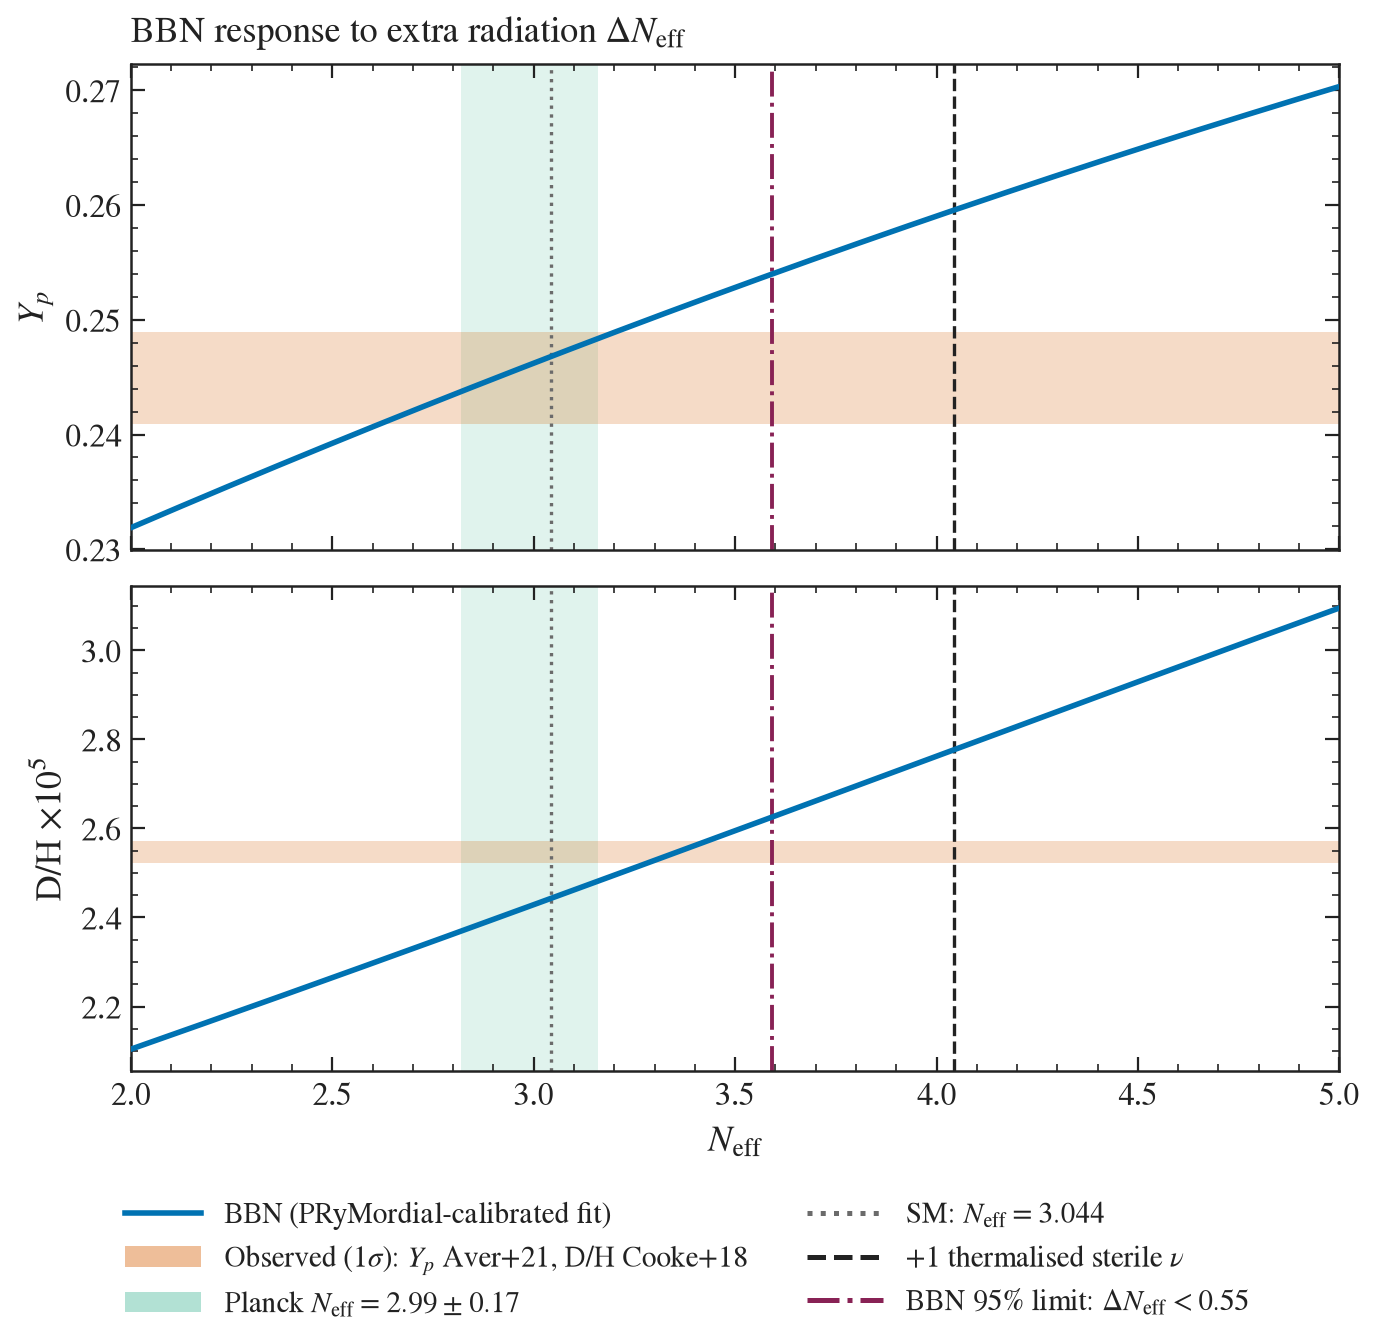
\includegraphics[width=0.85\textwidth,height=0.6\textheight,keepaspectratio]{fig-6.png}
\caption{bbn\_vs\_neff.png Produced in this session by \texttt{plot\_sterile\_nu\_bbn\_impact} on \textit{serve-sbbn.sh}.}
\label{fig:6}
\end{figure}

\begin{figure}[H]
\centering
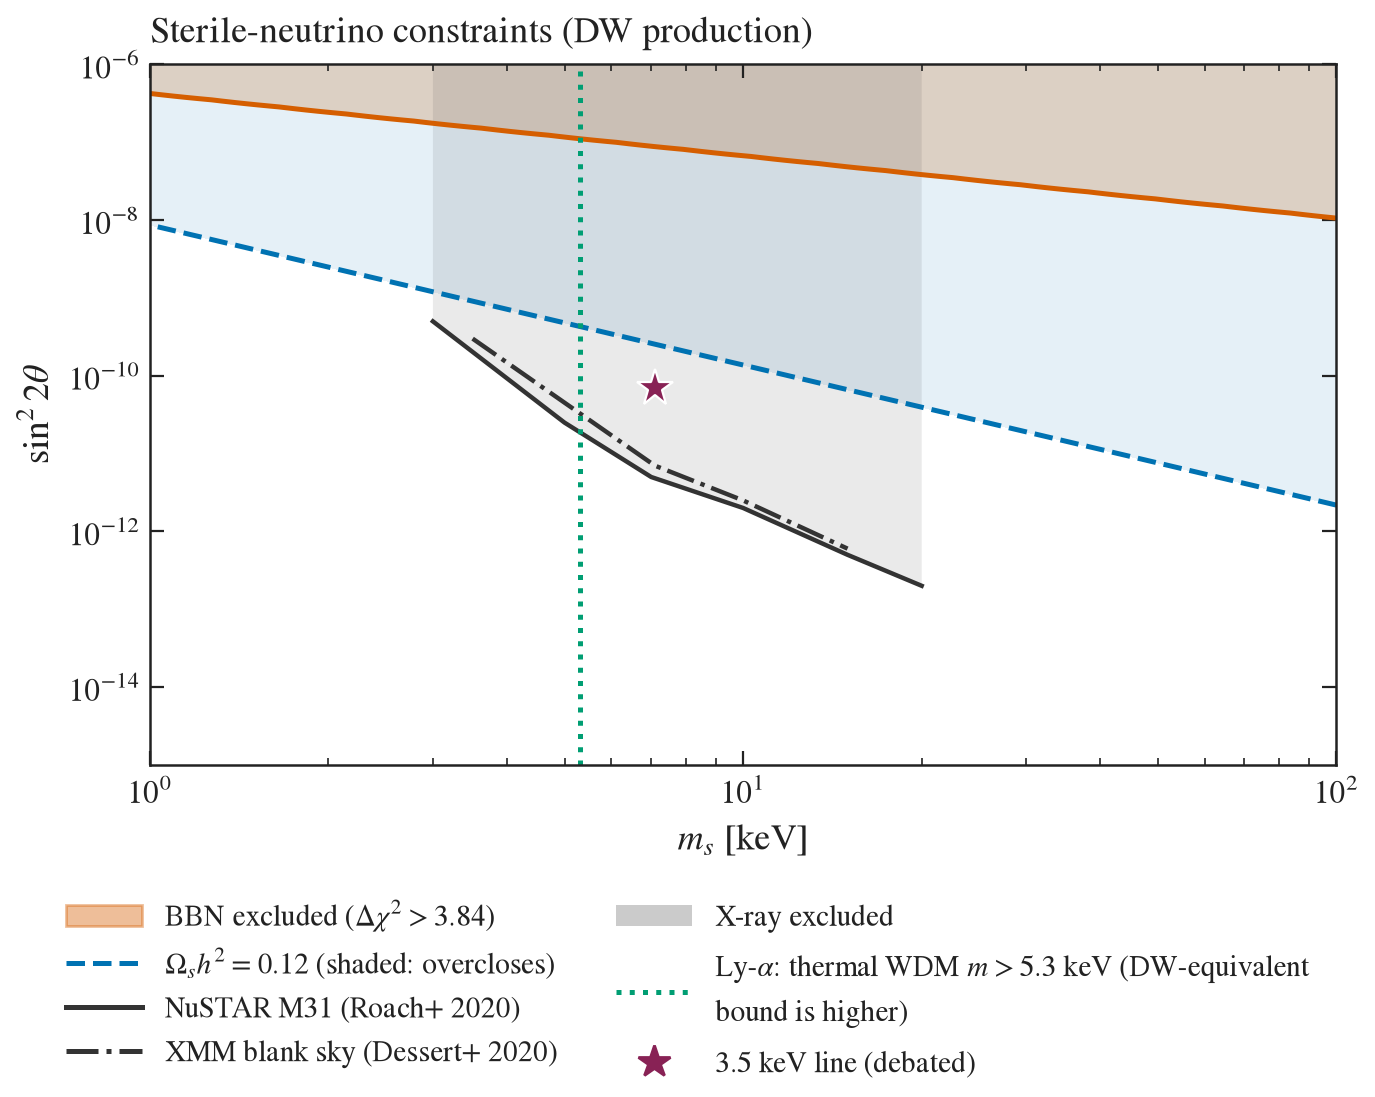
\includegraphics[width=0.85\textwidth,height=0.6\textheight,keepaspectratio]{fig-8.png}
\caption{exclusion\_scan\_DW\_dc7743.png Produced in this session by \texttt{plot\_sterile\_nu\_exclusion} on \textit{serve-sbbn.sh}.}
\label{fig:8}
\end{figure}

\begin{figure}[H]
\centering
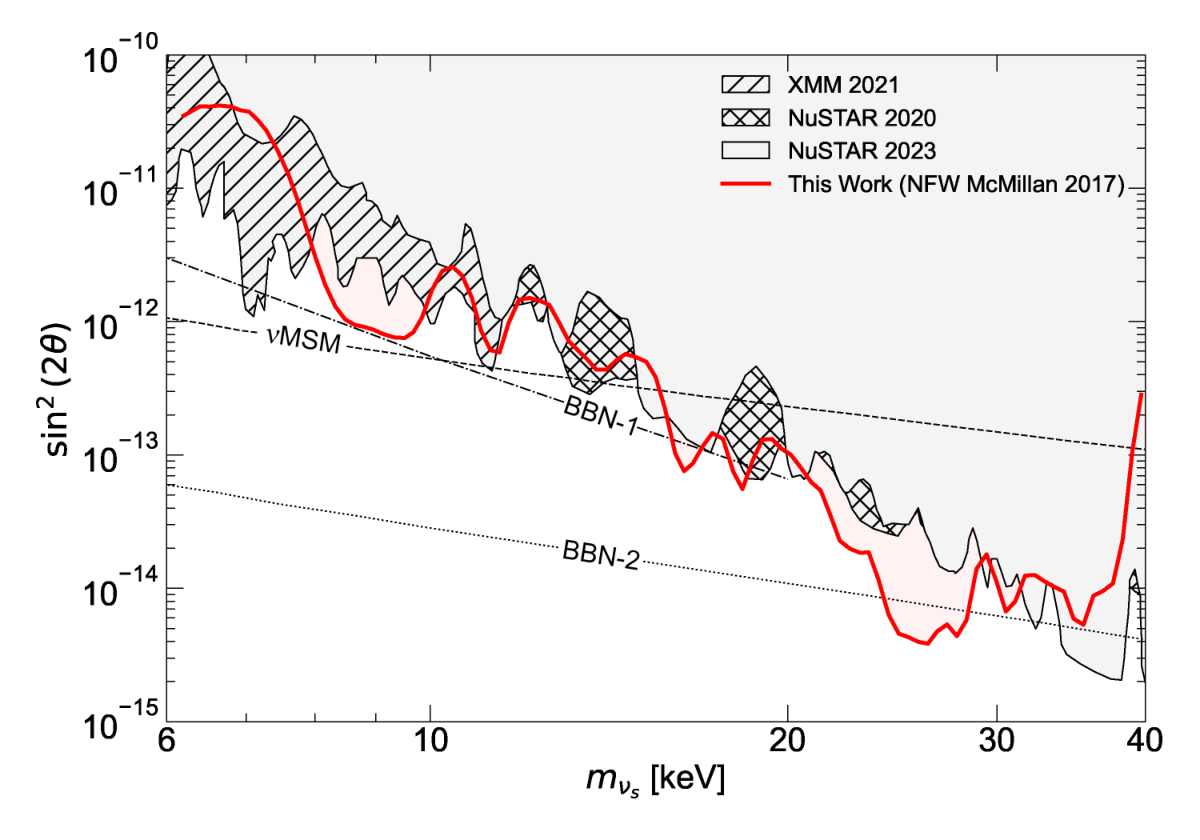
\includegraphics[width=0.85\textwidth,height=0.6\textheight,keepaspectratio]{fig-15.png}
\caption{Figure 1: 95\% upper limits on sin\textasciicircum{}\{2\}(2\textbackslash{}theta) derived from the NuSTAR unfocused stray light spectrum for reference profile [15] along with some previous constraints [9, NuSTAR 2020, 2023:], [16, XMM 2021:] and updated theoretical lower bounds [17, 18, 19]. Note that the borderline excess at 40 keV is the known instrumental effect caused by absorbed stray light [20, 21, 22]. [arXiv:2405.17861] Reproduced from arXiv:2405.17861 (extracted with \texttt{get\_paper\_figures}).}
\label{fig:15}
\end{figure}

\begin{figure}[H]
\centering
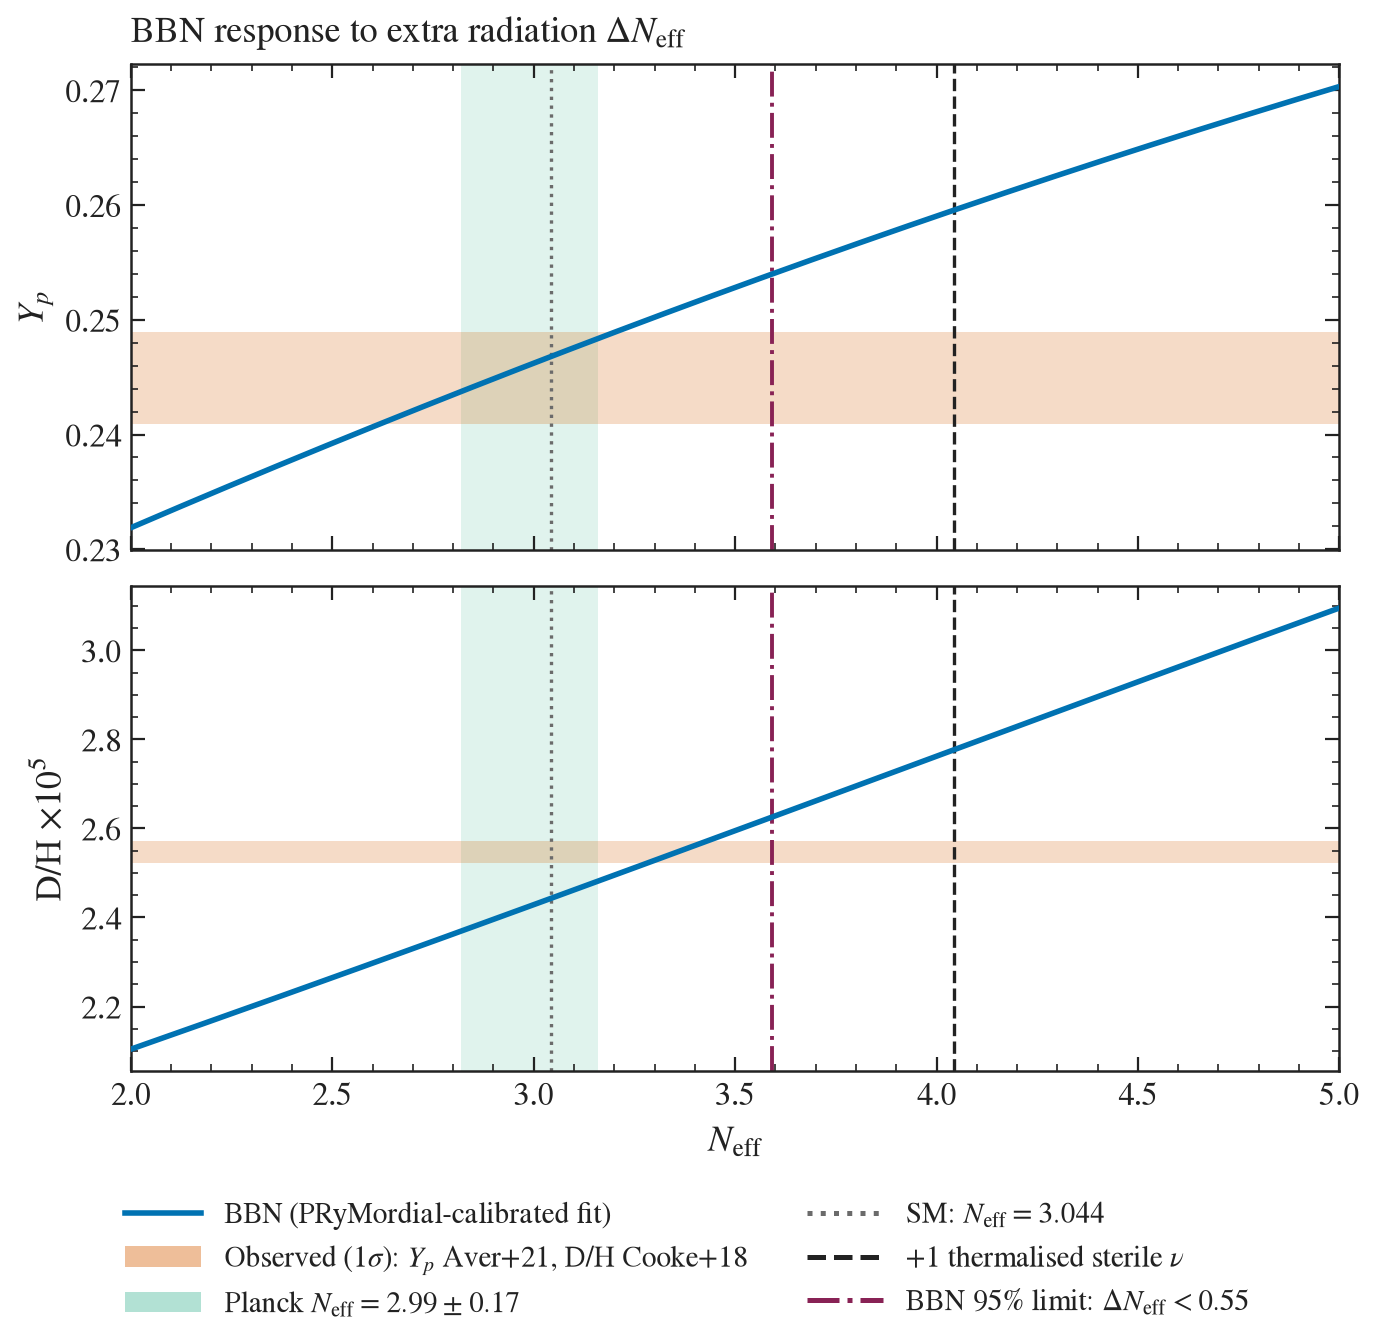
\includegraphics[width=0.85\textwidth,height=0.6\textheight,keepaspectratio]{fig-27.png}
\caption{bbn\_vs\_neff.png Produced in this session by \texttt{plot\_sterile\_nu\_bbn\_impact} on \textit{serve-sbbn.sh}.}
\label{fig:27}
\end{figure}

\begin{figure}[H]
\centering
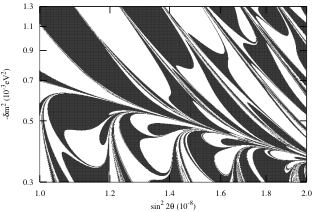
\includegraphics[width=0.85\textwidth,height=0.6\textheight,keepaspectratio]{fig-29.png}
\caption{Figure 2: Shown is the final sign of the lepton asymmetry as a function of mass splitting and mixing angle in the case of \textbackslash{}nu\_\{\textbackslash{}tau\}\textbackslash{}leftrightarrow\textbackslash{}nu\_\{s\} mixing for a specific range where arbitrary experimental accuracy could be unable to predict the sign of the lepton number of the Universe. White indicates a positive sign and black negative, from Ref. [114]. [arXiv:1705.01837] Reproduced from arXiv:1705.01837 (extracted with \texttt{get\_paper\_figures}).}
\label{fig:29}
\end{figure}

\begin{figure}[H]
\centering
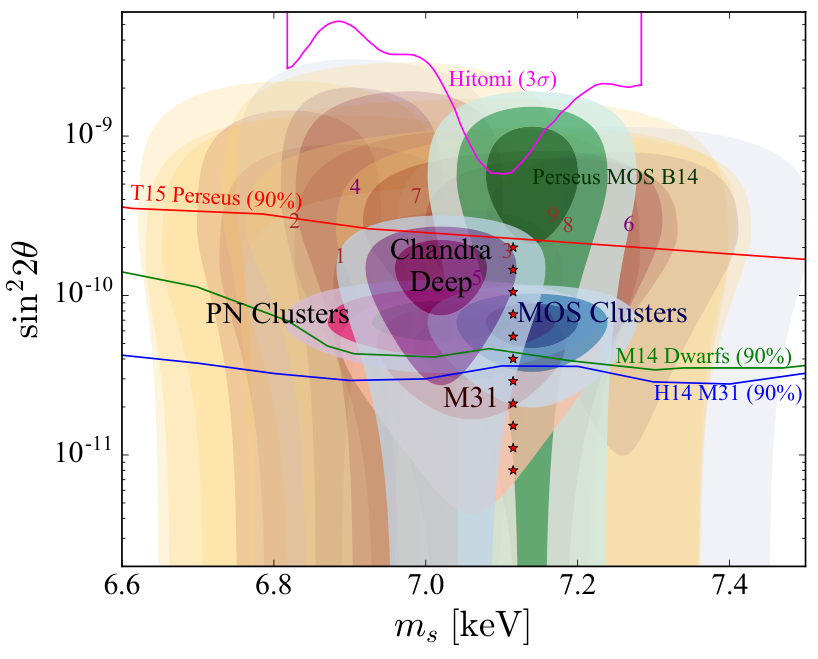
\includegraphics[width=0.85\textwidth,height=0.6\textheight,keepaspectratio]{fig-30.png}
\caption{Figure 7: X-ray line detections consistent with sterile neutrino dark matter are shown here. The dark colored regions are 1,2 and 3 \textbackslash{}sigma from the MOS (blue) and PN (red) stacked clusters by Bulbul et al. [29], the Bulbul et al. core-removed Perseus cluster (green), and M31 (orange) from Boyarsky et al. [30]. Also shown are the 1 and 2 \textbackslash{}sigma regions of the detection in the Galactic Center (GC) [210] as well as the \textgreater{}\textbackslash{}!2\textbackslash{}sigma line detections in 1. Abell 85; 2. Abell 2199; 3. Abell 496 (MOS); 4. Abell 496 (PN); 5. Abell 3266; 6. Abell S805; 7. Coma; 8. Abell 2319; 9. Perseus by Iakubovskyi et  [arXiv:1705.01837] Reproduced from arXiv:1705.01837 (extracted with \texttt{get\_paper\_figures}).}
\label{fig:30}
\end{figure}

\begin{figure}[H]
\centering
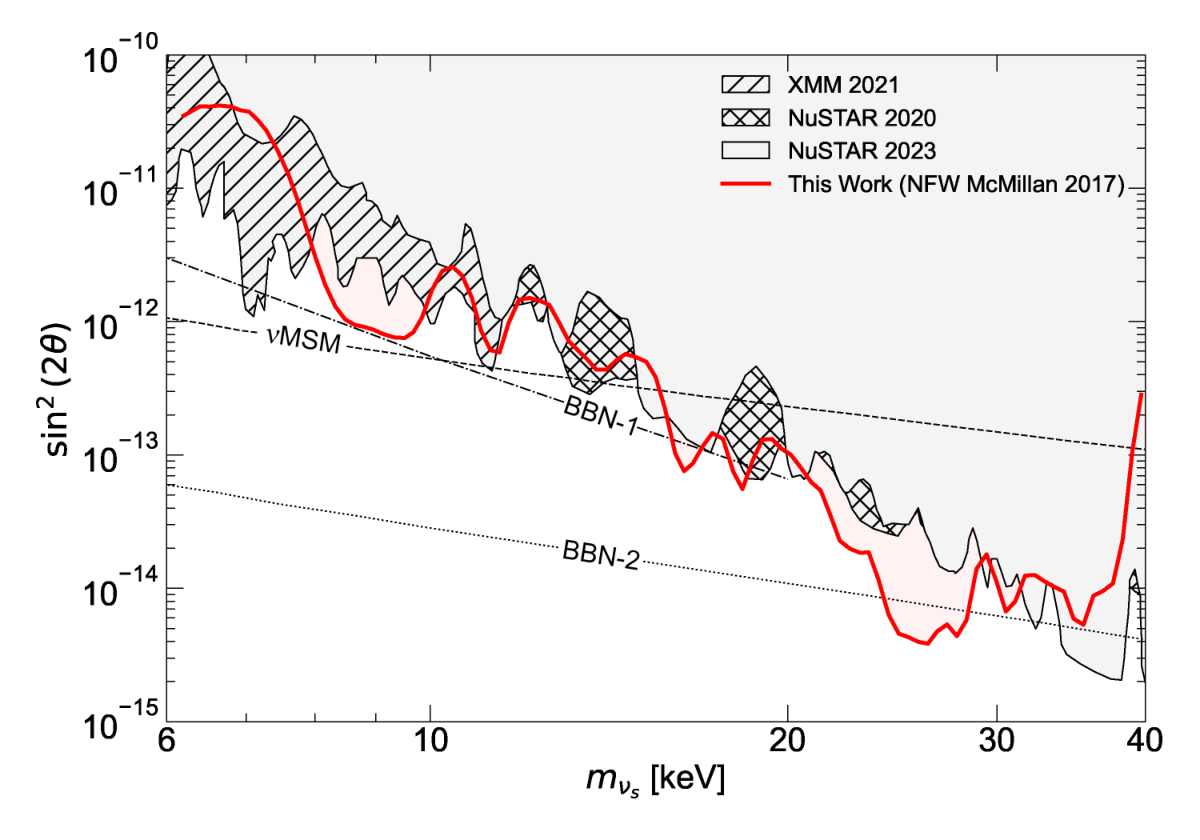
\includegraphics[width=0.85\textwidth,height=0.6\textheight,keepaspectratio]{fig-39.png}
\caption{Figure 1: 95\% upper limits on sin\textasciicircum{}\{2\}(2\textbackslash{}theta) derived from the NuSTAR unfocused stray light spectrum for reference profile [15] along with some previous constraints [9, NuSTAR 2020, 2023:], [16, XMM 2021:] and updated theoretical lower bounds [17, 18, 19]. Note that the borderline excess at 40 keV is the known instrumental effect caused by absorbed stray light [20, 21, 22]. [arXiv:2405.17861] Reproduced from arXiv:2405.17861 (extracted with \texttt{get\_paper\_figures}).}
\label{fig:39}
\end{figure}

\begin{figure}[H]
\centering
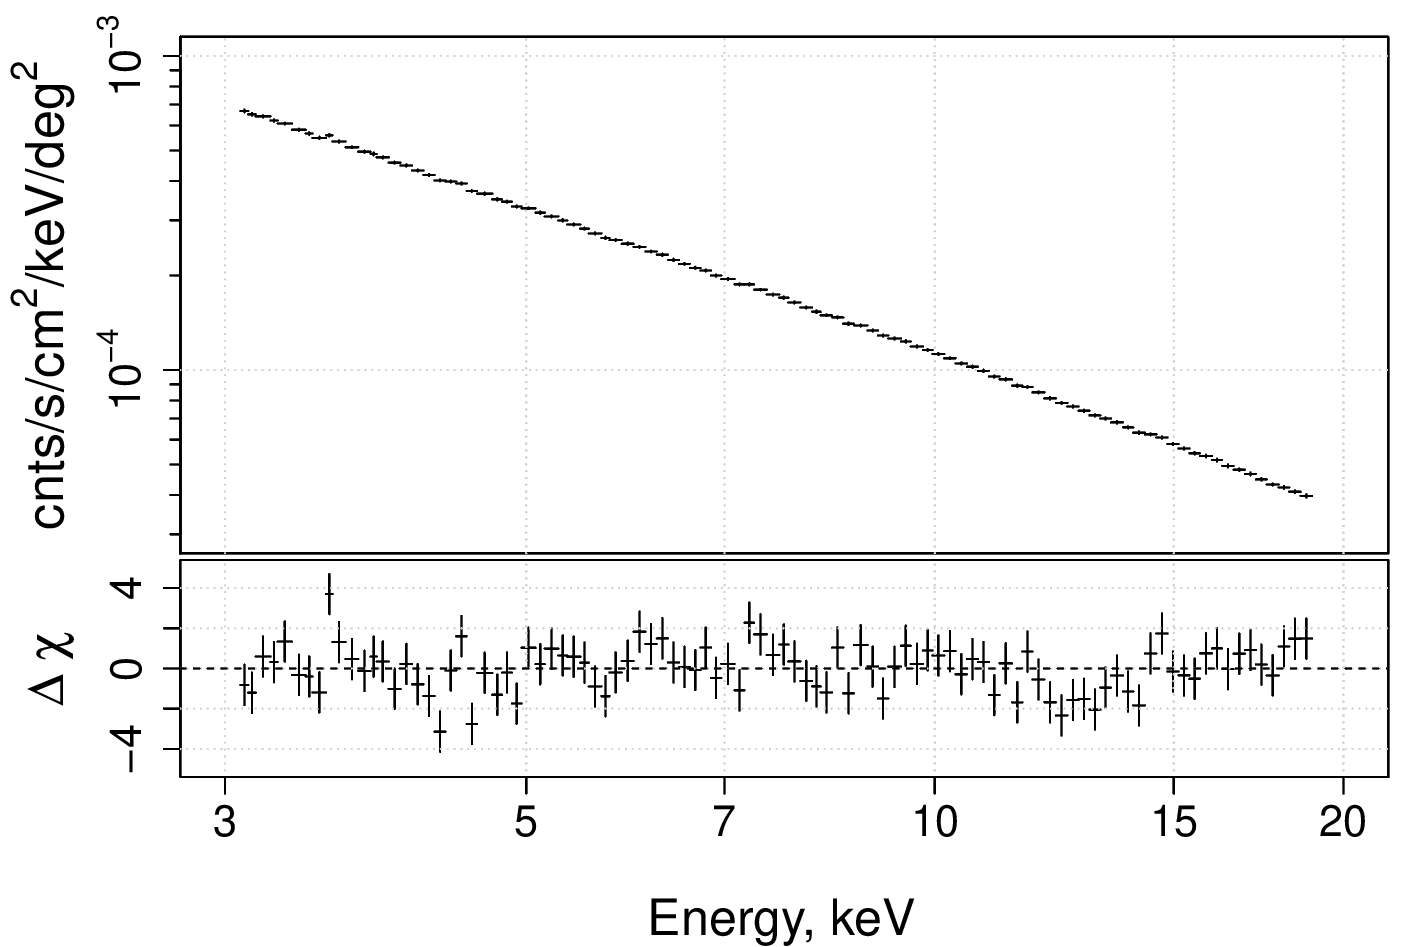
\includegraphics[width=0.85\textwidth,height=0.6\textheight,keepaspectratio]{fig-40.png}
\caption{Figure 2: The NuSTAR FPMA and FPMB combined spectrum of the unfocused stray light sky background, measured at \textbar{}b\textbar{}\textgreater{}3\textasciicircum{}\{\textbackslash{}circ\} (aCXB). Due to high statistics in each energy bin, we do not plot the total spectrum model in the upper panel for convenience. [arXiv:2405.17861] Reproduced from arXiv:2405.17861 (extracted with \texttt{get\_paper\_figures}).}
\label{fig:40}
\end{figure}

\begin{figure}[H]
\centering
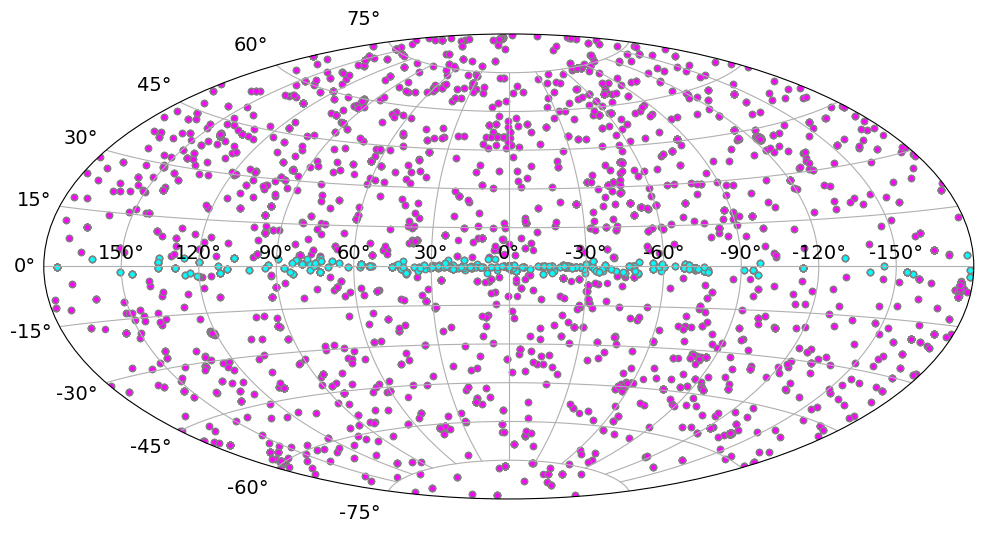
\includegraphics[width=0.85\textwidth,height=0.6\textheight,keepaspectratio]{fig-41.png}
\caption{Figure 4: The distribution of 3248 (FPMA) and 3139 (FPMB) NuSTAR observations on the sky in Galactic coordinates. Cyan and magenta points show the NuSTAR observations at \textbar{}b\textbar{}\textless{}3\textasciicircum{}\{\textbackslash{}circ\} and \textbar{}b\textbar{}\textgreater{}3\textasciicircum{}\{\textbackslash{}circ\}, respectively. [arXiv:2405.17861] Reproduced from arXiv:2405.17861 (extracted with \texttt{get\_paper\_figures}).}
\label{fig:41}
\end{figure}

\begin{figure}[H]
\centering
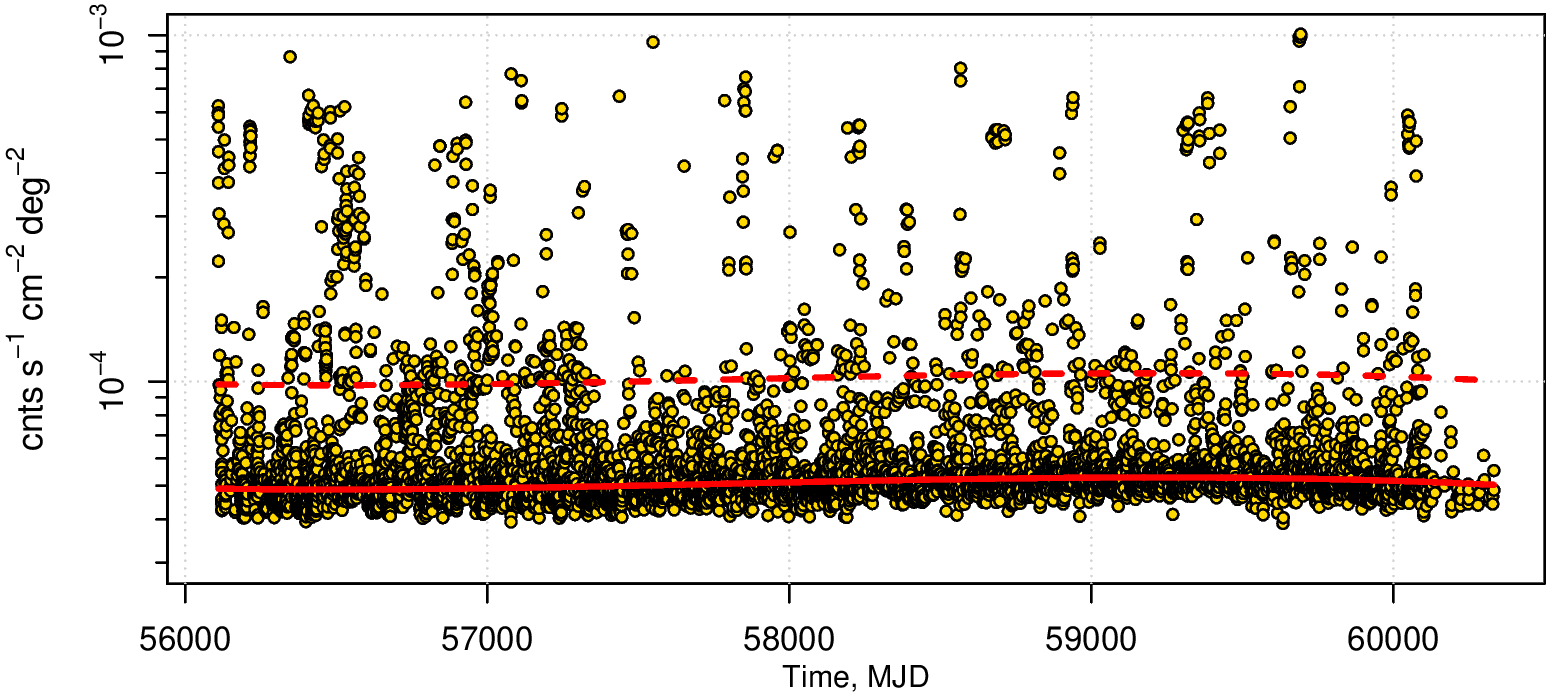
\includegraphics[width=0.85\textwidth,height=0.6\textheight,keepaspectratio]{fig-42.png}
\caption{Figure 5: The NuSTAR detector count rate as a function of time. Each point represents individual NuSTAR observation. A solid red line is a cubic polynomial outlier-resistant approximation used to describe long-term variation. A dashed red line shows the same approximation scaled by a factor of 2, that is a threshold: the observations above it are excluded from the analysis. [arXiv:2405.17861] Reproduced from arXiv:2405.17861 (extracted with \texttt{get\_paper\_figures}).}
\label{fig:42}
\end{figure}

\begin{figure}[H]
\centering
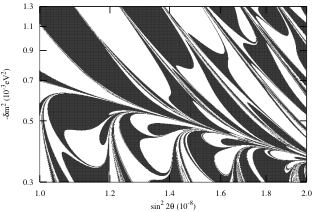
\includegraphics[width=0.85\textwidth,height=0.6\textheight,keepaspectratio]{fig-43.png}
\caption{Figure 2: Shown is the final sign of the lepton asymmetry as a function of mass splitting and mixing angle in the case of \textbackslash{}nu\_\{\textbackslash{}tau\}\textbackslash{}leftrightarrow\textbackslash{}nu\_\{s\} mixing for a specific range where arbitrary experimental accuracy could be unable to predict the sign of the lepton number of the Universe. White indicates a positive sign and black negative, from Ref. [114]. [arXiv:1705.01837] Reproduced from arXiv:1705.01837 (extracted with \texttt{get\_paper\_figures}).}
\label{fig:43}
\end{figure}

\begin{figure}[H]
\centering
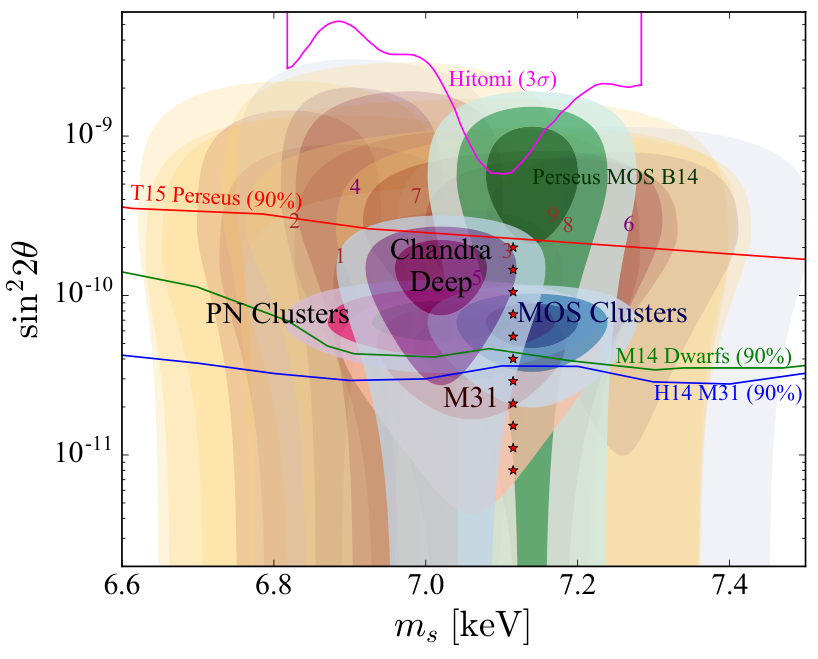
\includegraphics[width=0.85\textwidth,height=0.6\textheight,keepaspectratio]{fig-44.png}
\caption{Figure 7: X-ray line detections consistent with sterile neutrino dark matter are shown here. The dark colored regions are 1,2 and 3 \textbackslash{}sigma from the MOS (blue) and PN (red) stacked clusters by Bulbul et al. [29], the Bulbul et al. core-removed Perseus cluster (green), and M31 (orange) from Boyarsky et al. [30]. Also shown are the 1 and 2 \textbackslash{}sigma regions of the detection in the Galactic Center (GC) [210] as well as the \textgreater{}\textbackslash{}!2\textbackslash{}sigma line detections in 1. Abell 85; 2. Abell 2199; 3. Abell 496 (MOS); 4. Abell 496 (PN); 5. Abell 3266; 6. Abell S805; 7. Coma; 8. Abell 2319; 9. Perseus by Iakubovskyi et  [arXiv:1705.01837] Reproduced from arXiv:1705.01837 (extracted with \texttt{get\_paper\_figures}).}
\label{fig:44}
\end{figure}

\begin{figure}[H]
\centering
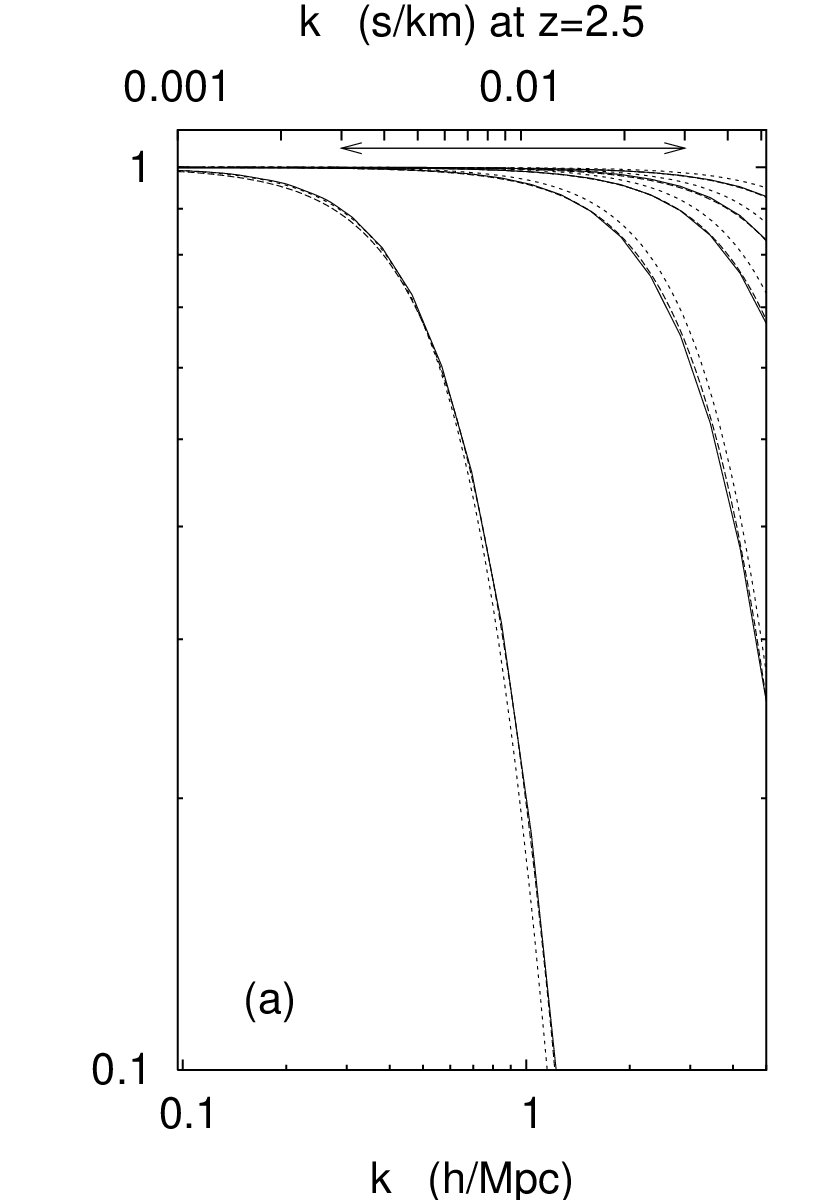
\includegraphics[width=0.85\textwidth,height=0.6\textheight,keepaspectratio]{fig-45.png}
\caption{Figure 1: The WDM transfer function T(k) defined in equation (4) for various models (all with the same cosmological parameters \textbackslash{}Omega\_\{\textbackslash{}mathrm\{B\}\}\textbackslash{}!=\textbackslash{}!0.05, \textbackslash{}Omega\_\{\textbackslash{}mathrm\{DM\}\}\textbackslash{}!=\textbackslash{}!0.25, \textbackslash{}Omega\_\{\textbackslash{}Lambda\}\textbackslash{}!=\textbackslash{}!0.70). (a) Pure \textbackslash{}LambdaWDM model with, from left to right, T\_\{x\}/T\_\{\textbackslash{}nu\}=0.5,0.3,0.25,0.226,0.2, corresponding to m\_\{x\}=92,427,738,1000,1441\textbackslash{},\textbackslash{}mathrm\{eV\}. The solid curves are obtained numerically, the long--dashed curves (essentially indistinguishable from the solid curves) show the analytical fits based on equation (7), the short--dashed curves those based on Ref. [7]. (b) Mixed \textbackslash{}LambdaCW [arXiv:astro-ph/0501562] Produced in this session by \texttt{get\_paper\_figures} on \textit{hep-research-aid}.}
\label{fig:45}
\end{figure}

\begin{figure}[H]
\centering
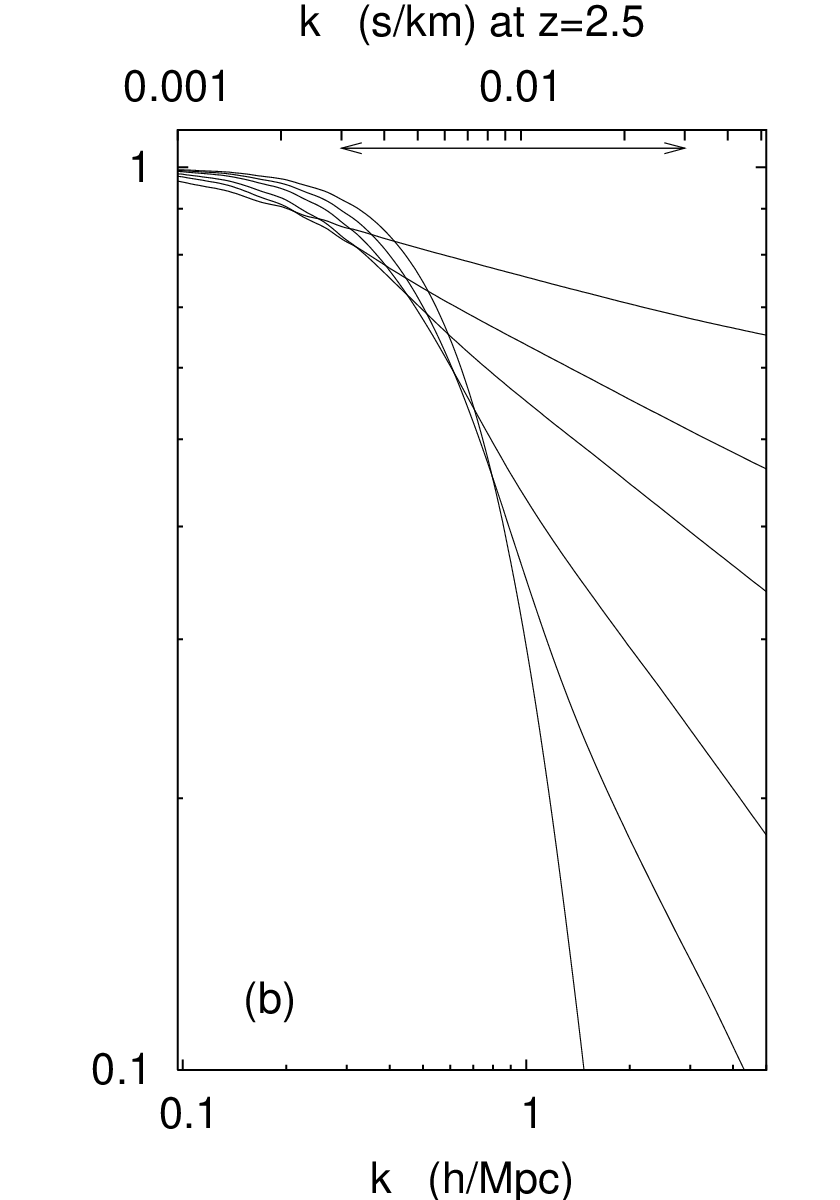
\includegraphics[width=0.85\textwidth,height=0.6\textheight,keepaspectratio]{fig-46.png}
\caption{Figure 1: The WDM transfer function T(k) defined in equation (4) for various models (all with the same cosmological parameters \textbackslash{}Omega\_\{\textbackslash{}mathrm\{B\}\}\textbackslash{}!=\textbackslash{}!0.05, \textbackslash{}Omega\_\{\textbackslash{}mathrm\{DM\}\}\textbackslash{}!=\textbackslash{}!0.25, \textbackslash{}Omega\_\{\textbackslash{}Lambda\}\textbackslash{}!=\textbackslash{}!0.70). (a) Pure \textbackslash{}LambdaWDM model with, from left to right, T\_\{x\}/T\_\{\textbackslash{}nu\}=0.5,0.3,0.25,0.226,0.2, corresponding to m\_\{x\}=92,427,738,1000,1441\textbackslash{},\textbackslash{}mathrm\{eV\}. The solid curves are obtained numerically, the long--dashed curves (essentially indistinguishable from the solid curves) show the analytical fits based on equation (7), the short--dashed curves those based on Ref. [7]. (b) Mixed \textbackslash{}LambdaCW [arXiv:astro-ph/0501562] Produced in this session by \texttt{get\_paper\_figures} on \textit{hep-research-aid}.}
\label{fig:46}
\end{figure}

\begin{figure}[H]
\centering
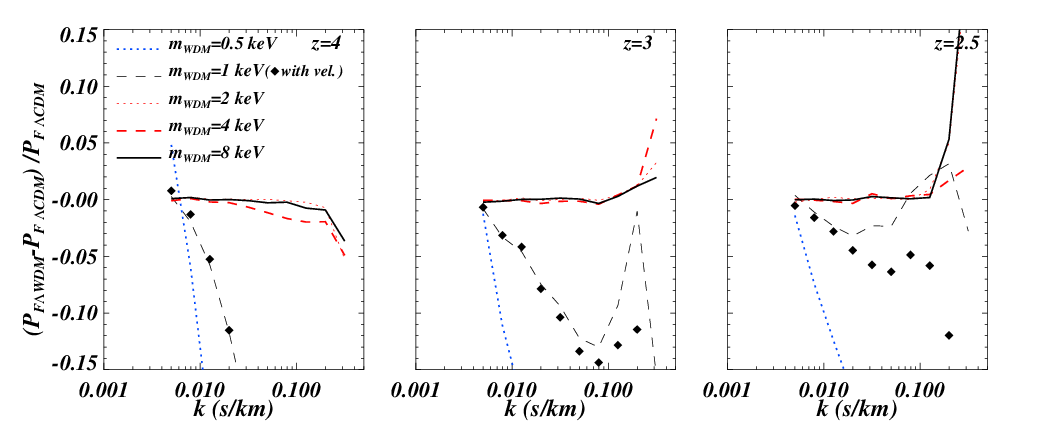
\includegraphics[width=0.85\textwidth,height=0.6\textheight,keepaspectratio]{fig-47.png}
\caption{Figure 2: Fractional difference of the flux power spectrum for a hydro-dynamical simulation of a \textbackslash{}LambdaWDM model and the flux power spectrum for a \textbackslash{}LambdaCDM model. The simulations have a box size of 30 h\textasciicircum{}\{-1\} Mpc and 2003 gas and 2003 dark matter particles. The results are for three different redshifts (z=4,3,2.5, respectively from left to right) and for five different values of the (thermal WDM) particle mass: 0.5 keV (thick dotted), 1 keV (thin dashed), 2 keV (thin dotted), 4 keV (thick dashed) and 8 keV (continuous). The diamonds show the results for a simulation with a WDM particle of ma [arXiv:astro-ph/0501562] Produced in this session by \texttt{get\_paper\_figures} on \textit{hep-research-aid}.}
\label{fig:47}
\end{figure}

\begin{figure}[H]
\centering
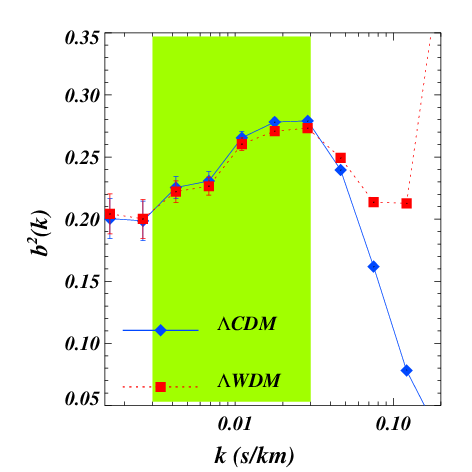
\includegraphics[width=0.85\textwidth,height=0.6\textheight,keepaspectratio]{fig-48.png}
\caption{Figure 3: Bias function b\textasciicircum{}\{2\}(k) between the flux power spectrum and the linear dark matter power spectrum, P\_\{F\}(k)=b\textasciicircum{}\{2\}(k)\textbackslash{},P(k), for two cosmological models: \textbackslash{}LambdaCDM (diamonds) and \textbackslash{}LambdaWDM (squares), with a (thermal WDM) particle mass m\_\{\textbackslash{}rm WDM\}=1 keV. The simulation has a boxsize of 60 comoving h\textasciicircum{}\{-1\}Mpc and 2\textbackslash{}times 400\textasciicircum{}\{3\} (gas and dark matter) particles (see Section III.2 for further details on other simulation parameters). The shaded area indicates the range of wavenumbers used in our analysis. [arXiv:astro-ph/0501562] Produced in this session by \texttt{get\_paper\_figures} on \textit{hep-research-aid}.}
\label{fig:48}
\end{figure}

\begin{figure}[H]
\centering
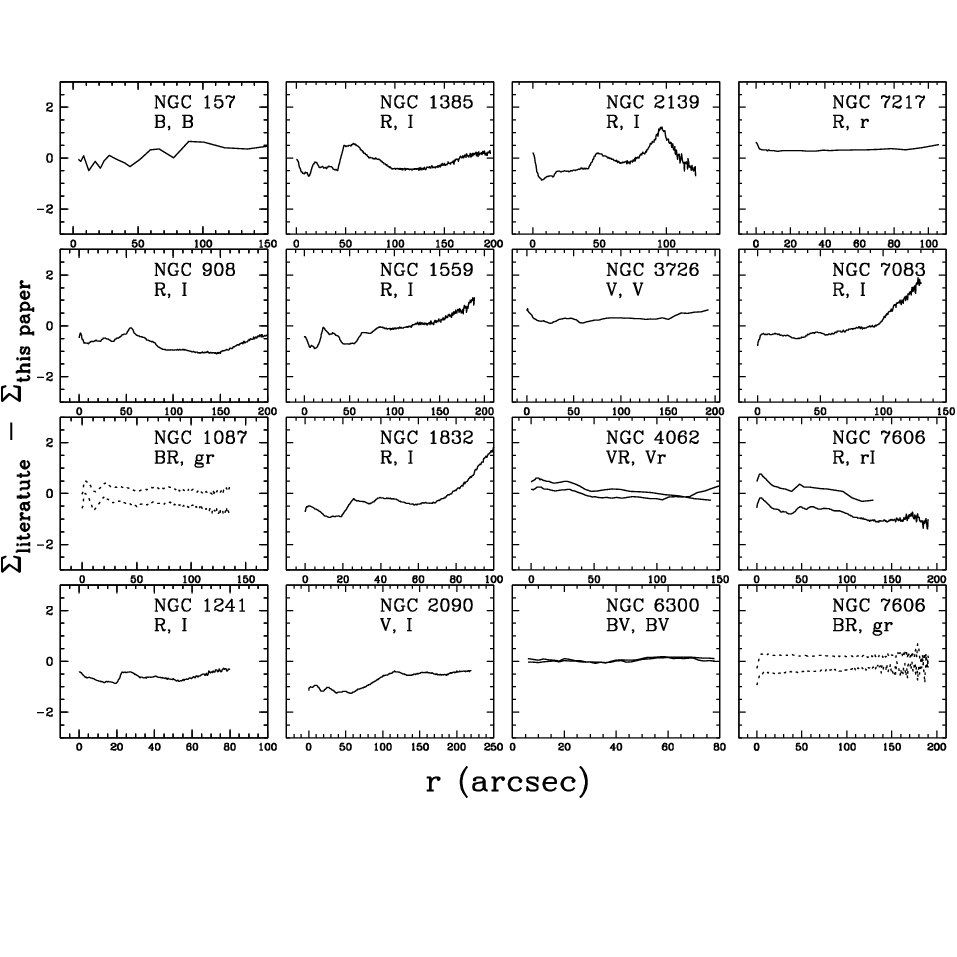
\includegraphics[width=0.85\textwidth,height=0.6\textheight,keepaspectratio]{fig-49.png}
\caption{Figure 2: Surface brightness profiles from this paper are compared to those in the literature (solid lines) and the SDSS DR2 (short dashed lines). Under the galaxy's NGC number, the band(s) of the surface brightness profile(s) plotted from this paper is(are) noted first, then the band(s) from the literature/SDSS DR2 are(are) noted after. [arXiv:astro-ph/0602028] Produced in this session by \texttt{get\_paper\_figures} on \textit{hep-research-aid}.}
\label{fig:49}
\end{figure}

\begin{figure}[H]
\centering
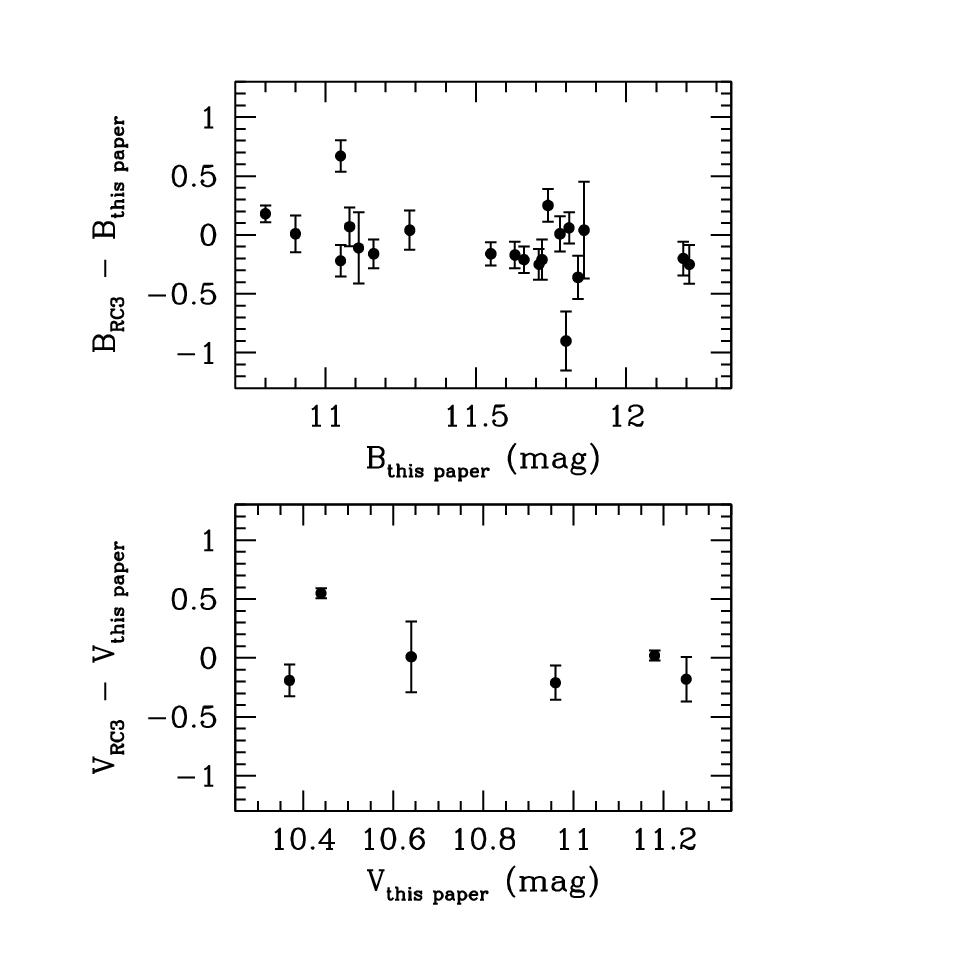
\includegraphics[width=0.85\textwidth,height=0.6\textheight,keepaspectratio]{fig-50.png}
\caption{Figure 3: We plot the difference between the total integrated RC3 magnitudes and the integrated magnitudes from this paper versus magnitudes from this paper. In the upper panel we compare the B-band magnitudes, and in the lower panel we compare the V-band magnitudes. [arXiv:astro-ph/0602028] Produced in this session by \texttt{get\_paper\_figures} on \textit{hep-research-aid}.}
\label{fig:50}
\end{figure}

\begin{figure}[H]
\centering
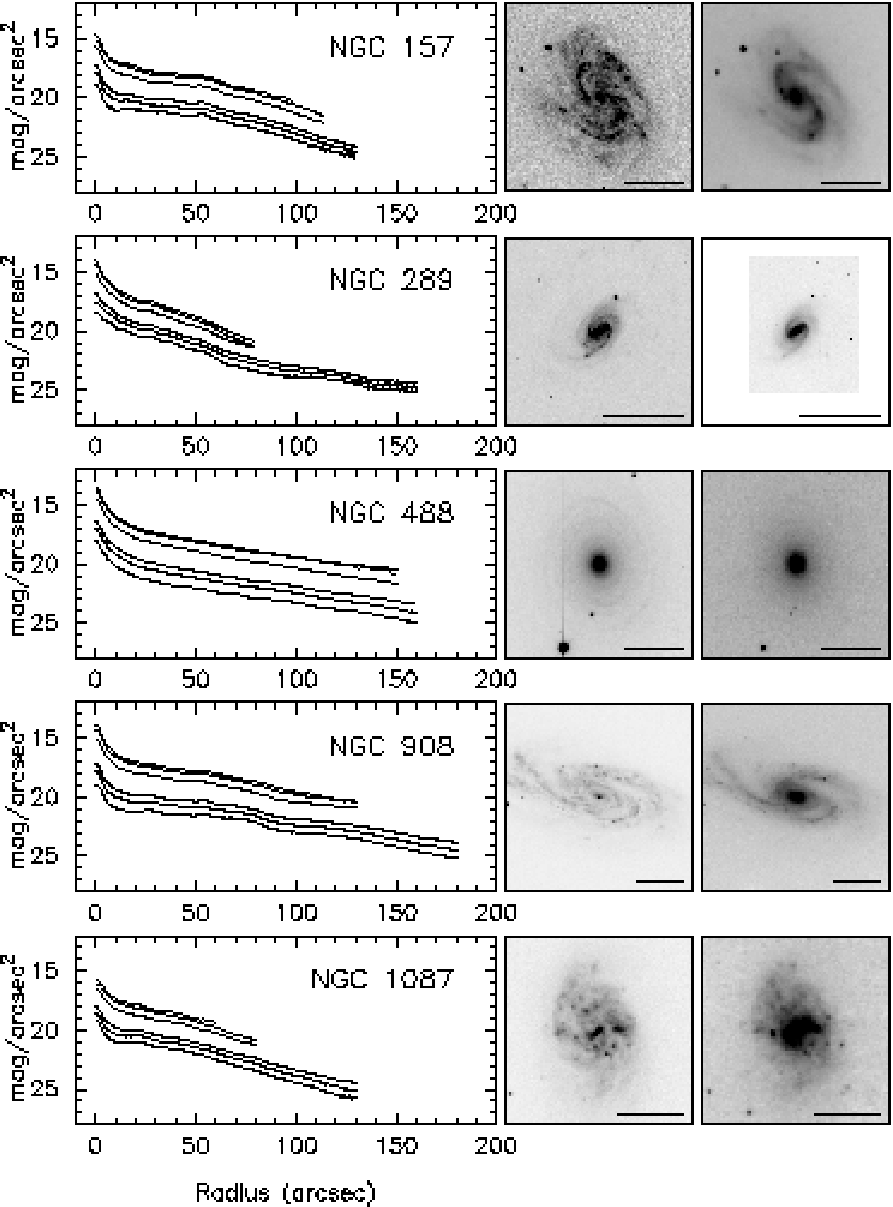
\includegraphics[width=0.85\textwidth,height=0.6\textheight,keepaspectratio]{fig-51.png}
\caption{Figure 1a: Observed surface brightness profiles and B and K-band images for the sample galaxies. In this and subsequent figures, surface brightness curves run B-to-K bottom-to-top; see Table 2 for the observed bands. The B image is on the left, K on the right, and the scale bar indicates 60?. Orientation is North=Up, East=Left. Degraded resolution for astro-ph; please see journal article or send an email for a version at a higher resolution. [arXiv:astro-ph/0602028] Produced in this session by \texttt{get\_paper\_figures} on \textit{hep-research-aid}.}
\label{fig:51}
\end{figure}

\begin{figure}[H]
\centering
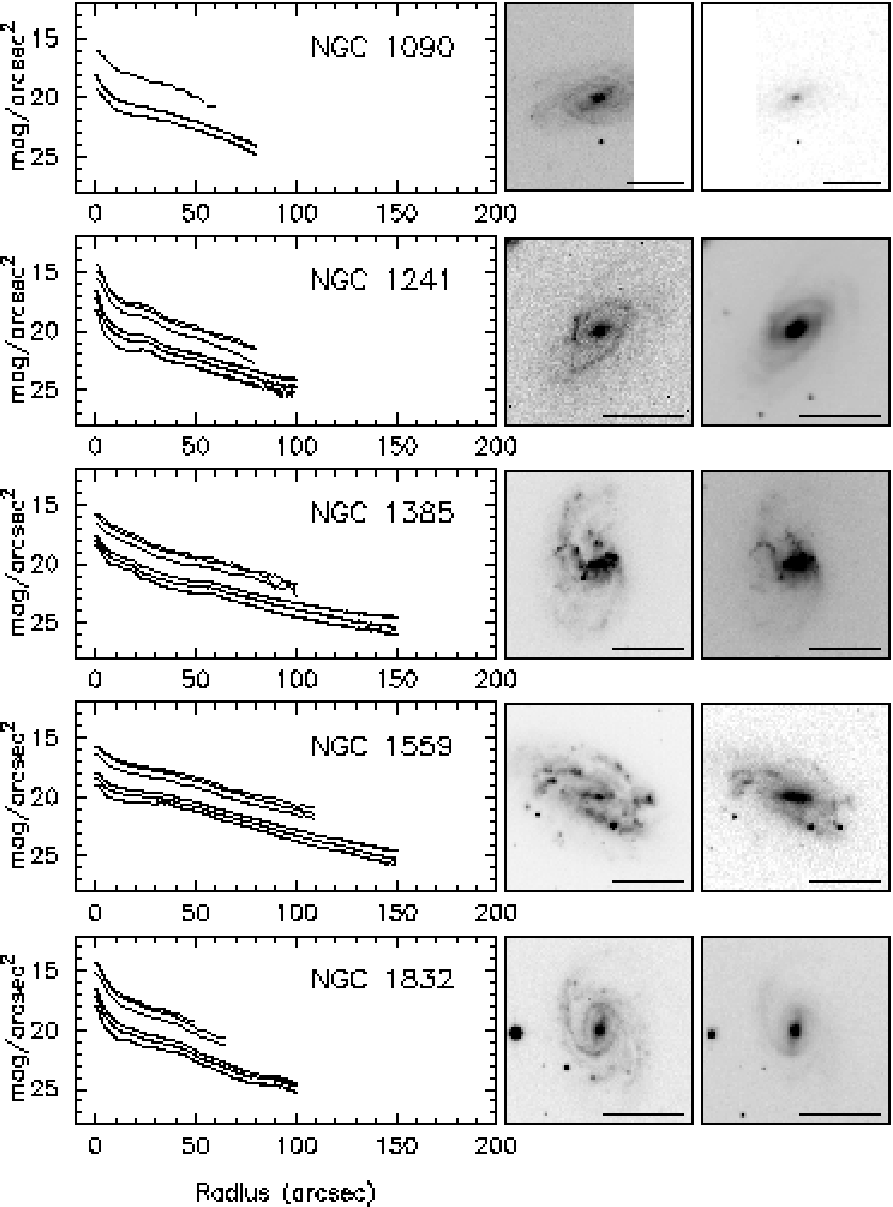
\includegraphics[width=0.85\textwidth,height=0.6\textheight,keepaspectratio]{fig-52.png}
\caption{Figure 1b: See Figure 1a. [arXiv:astro-ph/0602028] Produced in this session by \texttt{get\_paper\_figures} on \textit{hep-research-aid}.}
\label{fig:52}
\end{figure}

\end{document}
